\documentclass[sigconf, anonymous]{acmart}

\fancyhf{} % Remove fancy page headers 
\fancyhead[C]{Anonymous submission to ICISC 2017} % TODO: replace 9999 with your paper number
\fancyfoot[C]{\thepage}

\usepackage{graphicx}
\usepackage{booktabs}
\usepackage{soul}


\setcopyright{none} % No copyright notice required for submissions
\acmConference[Anonymous Submission to ICISC 2017]{The 20th Annual International Conference on Information Security and Crytology}{Due October 8, 2017}{Seoul, Korea}
\acmYear{2017}

\settopmatter{printacmref=false, printccs=true, printfolios=true} % We want page numbers on submissions

%%\ccsPaper{9999} % TODO: replace with your paper number once obtained

\begin{document}
\title{Detecting Phone Theft Using Machine Learning} % TODO: replace with your title

\begin{abstract}
Millions of smartphones are stolen in the United States every year, putting victims' personal information at risk since many users often do not lock their phones. 
To protect individuals' smartphones and the private data stored on them, we developed a system that automatically detects pickpocket and grab-and-run theft, in which a thief grabs the phone from a victim's hand then runs away. 
Our system applies machine learning to smartphone accelerometer data in order to detect possible theft incidents. Based on a field study and simulated theft scenarios, we are able to detect all thefts at a cost of 1 false alarm per week. Given that many smartphone users refuse to enable screen locking mechanisms over complaints that it takes too long to unlock their devices, our system could be used in conjunction with these systems in order to drastically decrease the number of times a user is asked to provide a lock code. That is, our system could be used to prompt smartphone users for PINs or passcodes only when theft events have been detected.
\end{abstract}

% % TODO: replace this section with code generated by the tool at https://dl.acm.org/ccs.cfm
% \begin{CCSXML}
% <ccs2012>
% <concept>
% <concept_id>10002978.10003014.10003017</concept_id>
% <concept_desc>Security and privacy~Mobile and wireless security</concept_desc>
% <concept_significance>500</concept_significance>
% </concept>
% <concept>
% <concept_id>10002978.10002991.10002992.10003479</concept_id>
% <concept_desc>Security and privacy~Biometrics</concept_desc>
% <concept_significance>300</concept_significance>
% </concept>
% </ccs2012>
% \end{CCSXML}

% \ccsdesc[500]{Security and privacy~Mobile and wireless security}
% \ccsdesc[300]{Security and privacy~Biometrics}
% % -- end of section to replace with generated code

\keywords{usable security, machine learning, smartphone theft detection} % TODO: replace with your keywords

\maketitle

\section{Introduction}

According to Consumer Reports, 2.1 million smartphones were stolen in the United States in 2014~\cite{deitrick:consumer}, and the Pew Research Center's Internet \& American Life Project reported in 2012 that nearly one third of mobile phone users have experienced a lost or stolen devices~\cite{boyles:pew}.
People can lock their phones to mitigate the risks of phone theft, but some find this less convenient as it requires unlocking their phone every time they want to use their phone.
About 40\% of smartphone users do not lock their phones, which allows thieves to gain access to the victims' personal information~\cite{egelman:lock}.

In this paper, we develop a method to automatically detect pickpocket and grab-and-run smartphone theft. To be more specific, we train a binary classifier to recognize the movements that are specific to theft and use it monitor accelerometer data in the background.
When theft is detected, it can signal the device to lock the phone and optionally notify the owner. Thus, our theft detector offers another layer of protection against smartphone theft.
Because our detector is completely automatic, it is convenient for users.

There are multiple ways that a phone might be stolen.
We focus specifically on grab-and-run theft, where the thief snatches the phone out of the user's hand and runs away, and pickpocket theft, where the thief steals the phone from the user's pocket or bag and runs away.
This creates an abrupt and unusual movement pattern, which we show can be detected from analysis of accelerometer sensor data.
We do not attempt to detect other forms of theft, such as where the phone is left unattended and the thief walks off with it, or where the phone is lost or left behind somewhere.
Consequently, our scheme cannot offer comprehensive protection against all forms of theft, but we hope that it will be useful nonetheless.

We measure the effectiveness of our scheme by gathering two datasets.
First, we simulated three types of phone theft: grab-and-run while the victim is standing still, grab-and-run while the victim is walking at a constant speed, and pick-pocket theft.
We collect accelerometer sensor readings during the simulated thefts; these serve as known positives.
Second, we conducted a field study where we collected 3 weeks of sensor readings from the phones of 53 participants during their everyday life.
No phone was stolen during the field study, so these serve as known negatives.
We use this to train a classifier and then evaluate its detection rate and false positive rate.
Our best classifier produces 1 false alarm per week on average while detecting 100\% of simulated thefts.


Our contributions are:
\begin{enumerate}
  \item We conduct a user study and collect a large dataset of smartphone sensor data while devices are being used in real world.
  \item We devise features and methods to detect theft, and we show that it can detect thefts with few false positives.
\end{enumerate}

\section{Related Work}

Many researchers have studied using smartphone sensors for continuous user authentication.
The benefit of continuous user authentication is that it happens unobtrusively, without requiring any action from users.
Continuous authentication could serve as a mitigation for theft: if the phone can detect rapidly enough that it is no longer being used by the rightful owner, it could lock itself to prevent the thief from accessing sensitive data on the phone. 

One approach is to use smartphone accelerometer data for gait recognition.
These systems often extract some features from the sensor data and then apply machine learning.
Derawi et~al.\ achieved an equal error rate of 20\%~\cite{derawi:gait}.
``Equal error rate'' is a measure of accuracy where the system is tuned so the false accept rate and false reject rates are equal, and then that error rate is reported.
Primo et~al.\ show that accelerometer-based gait authentication is somewhat dependent on the position in which the phone is held, which is a challenge for deploying gait authentication outside of a laboratory environment~\cite{primo:context}. 
They showed how to infer the position of the phone (in the person's hand vs.\ in a pocket) with 85\% accuracy, and they showed how to use this information to increase the accuracy of user authentication to 70--80\%.
They do not report performance as equal error rate.
Juefei-Xu et~al.\ show that the pace at which people walk also affects the sensor readings, and it is possible to improve accuracy by first identifying the pace at which the user is walking, then using a model tailored towards that pace~\cite{xu:pace}.
Their system achieved an equal error rate of 4--8\% (depending on the pace); or a false reject rate of 0.5--5\% at a false accept rate of 0.1\%.
Kwapisz et~al.\ generalized gait authentication to cover not just walking but also jogging and ascending and descending stairs~\cite{kwapisz:biometrics} and
achieved false reject rates of 10--15\% at a false accept rate of about 5\%.

It is not clear whether gait recognition is sufficient on its own for deployable user authentication.
One limitation is that it can only attempt to authenticate the user while the user is walking; when the user is still, it cannot infer user identity.
Another limitation is that the error rate is still fairly high: if the classifier is run continuously, once per second, even a false reject rate as low as 0.5\% will cause hundreds or thousands of false rejections per week.
Thus, gait recognition might need to be combined with other methods to yield a deployable defense against theft.

Our work builds on the methods previous researchers have used to process sensor data and extract features.
The accelerometer sensor provides raw data in the form of $X,Y,Z$ accelerations; it is useful to also compute the magnitude $M=\sqrt{X^2+Y^2+Z^2}$ of the acceleration, as that is independent of the direction of the acceleration.
Prior papers have used several methods for cleaning the raw accelerometer data, including interpolation and re-sampling to deal with irregularly sampled data and a weighted moving average filter to mitigate sensor noise.
These schemes typically divide the resulting time series into windows, each window containing about a second of sensor data.
For instance, Primo et~al.\ used overlapping windows, with each window containing 100 samples and having an overlap of 50 samples with the next window; Derawi et~al.\ and Juefei-Xu et~al.\ used non-overlapping windows, which were about 1 second in width.
Derawi et~al.\ and Juefei-Xu et~al.\ used the sensor readings as the features, while Primo et~al.\ and Kwapisz et~al.\ computed hand-crafted features from the readings, where each feature records a summary statistic on the sensor readings in the window (e.g., mean, minimum, maximum, standard deviation, number of zero crossings, etc.).

Feng et~al.\ investigated using the unique way the user picks up their phone as a biometric for user authentication~\cite{feng:pickup}. 
They achieved an equal error rate of 6--7\%.
They used the smartphone accelerometer, gyroscope, and magnetometer; in our work, we avoid the gyroscope sensor, as its power consumption is significantly higher than the accelerometer, and therefore is currently not a practical solution for continuous authentication.

Mare et~al.\ developed a continuous authentication system where the user wears a smartwatch or bracelet, which is used to authenticate the user to their computer~\cite{mare:zebra}. 
Their continuous authentication scheme works well and could plausibly be used to authenticate to a smartphone, but it requires users to wear a bracelet; in contrast, we seek solutions that do not require the user to carry or wear any additional devices.

The most closely related work is by Chang et~al.\, who used the way
that each person takes their phone out of their bag or pocket as a 
form of biometric authentication~\cite{cheng:theft}.
They use accelerometer and gyroscope data to detect when the user picks
up their phone, and then they apply dynamic time warping and boosting to
determine whether the pickup motion matches known templates from the
owner of the phone.
Their system achieves a 10\% false positive rate and a 5.5\% false negative rate, which are relatively high,
considering that users may pick up their phones dozens of times each day.

The prior work focuses on authenticating the user.
In contrast, we take a different approach: we attempt to detect the
specific motion pattern that occurs during a grab-and-run or pickpocket theft.
The benefit of biometric authentication is that it provides a comprehensive
way to detect theft, regardless of the way the phone was stolen; however,
as summarized above, the false positive rates of existing schemes
are fairly high.
Our scheme is limited to detecting a particular type of theft, but achieves
far lower false positive rates.
Our classifier is also user-independent and does not require obtaining
training data from each user; we use the same classifier for all users.




\section{Methodology}

In this section, we describe the data collection software, which we used to gather positive and negative data for our training and test sets as well as the feature extraction scheme, and other classifier design decisions.

\subsection{Data Collection}

\subsubsection{Software}
We used an Android application to record data from the smartphone's 3-axis accelerometer, which then encrypted it and stored it in the cloud.
We acquired sensor data at the highest sampling rate supported by the phone using SENSOR\_DELAY\_\\FASTEST~\cite{android:doc}. 
On most devices, including the one we used for the simulated theft experiment, the sampling rate is 100 Hz. 

\subsubsection{Simulated Theft Experiment}
Because data from real thefts is hard to obtain, we simulated three types of common smartphone theft scenarios, based on campus police alerts that we receive, with one researcher acting as a smartphone user and another one playing the role of a thief. 
The three theft scenarios are as follows:
\begin{enumerate}
\item The user stands still and holds the phone with one hand as she is using the device, for instance reading a text; the thief approaches from behind, grabs the phone with both hands and runs away in the forward direction. 
\item The user holds the phone in front of her with one hand while walking at a constant speed; the thief approaches from behind, grabs the phone with both hands and runs away in the forward direction. 
\item The third scenario simulates pick-pocket thefts. The user places the phone in the back pocket of their pants and stands still; the thief approaches from behind, steals the phone from user's pocket and runs away in the forward direction.
\end{enumerate}
We collect 40 instances of each scenario, for a total of 120 trials. 
Data collection was split across four sessions, each consisting of 10 trials per scenario, with different researchers acting as the victim and thief in these two sessions. 
We ran the experiment on flat ground in an open space, so the experiment was not interrupted. 
We also made sure that the thief ran at least 40 feet after gaining possession of the victim's phone.
We used a Nexus 5X smartphone (InvenSense MPU6515 embedded accelerometer) with Android version 7.1.1 for data collection in our simulated theft experiment.
Figure~\ref{fig:simtheft} plots one example of accelerometer readings from a single simulated theft.


\begin{figure}[t]
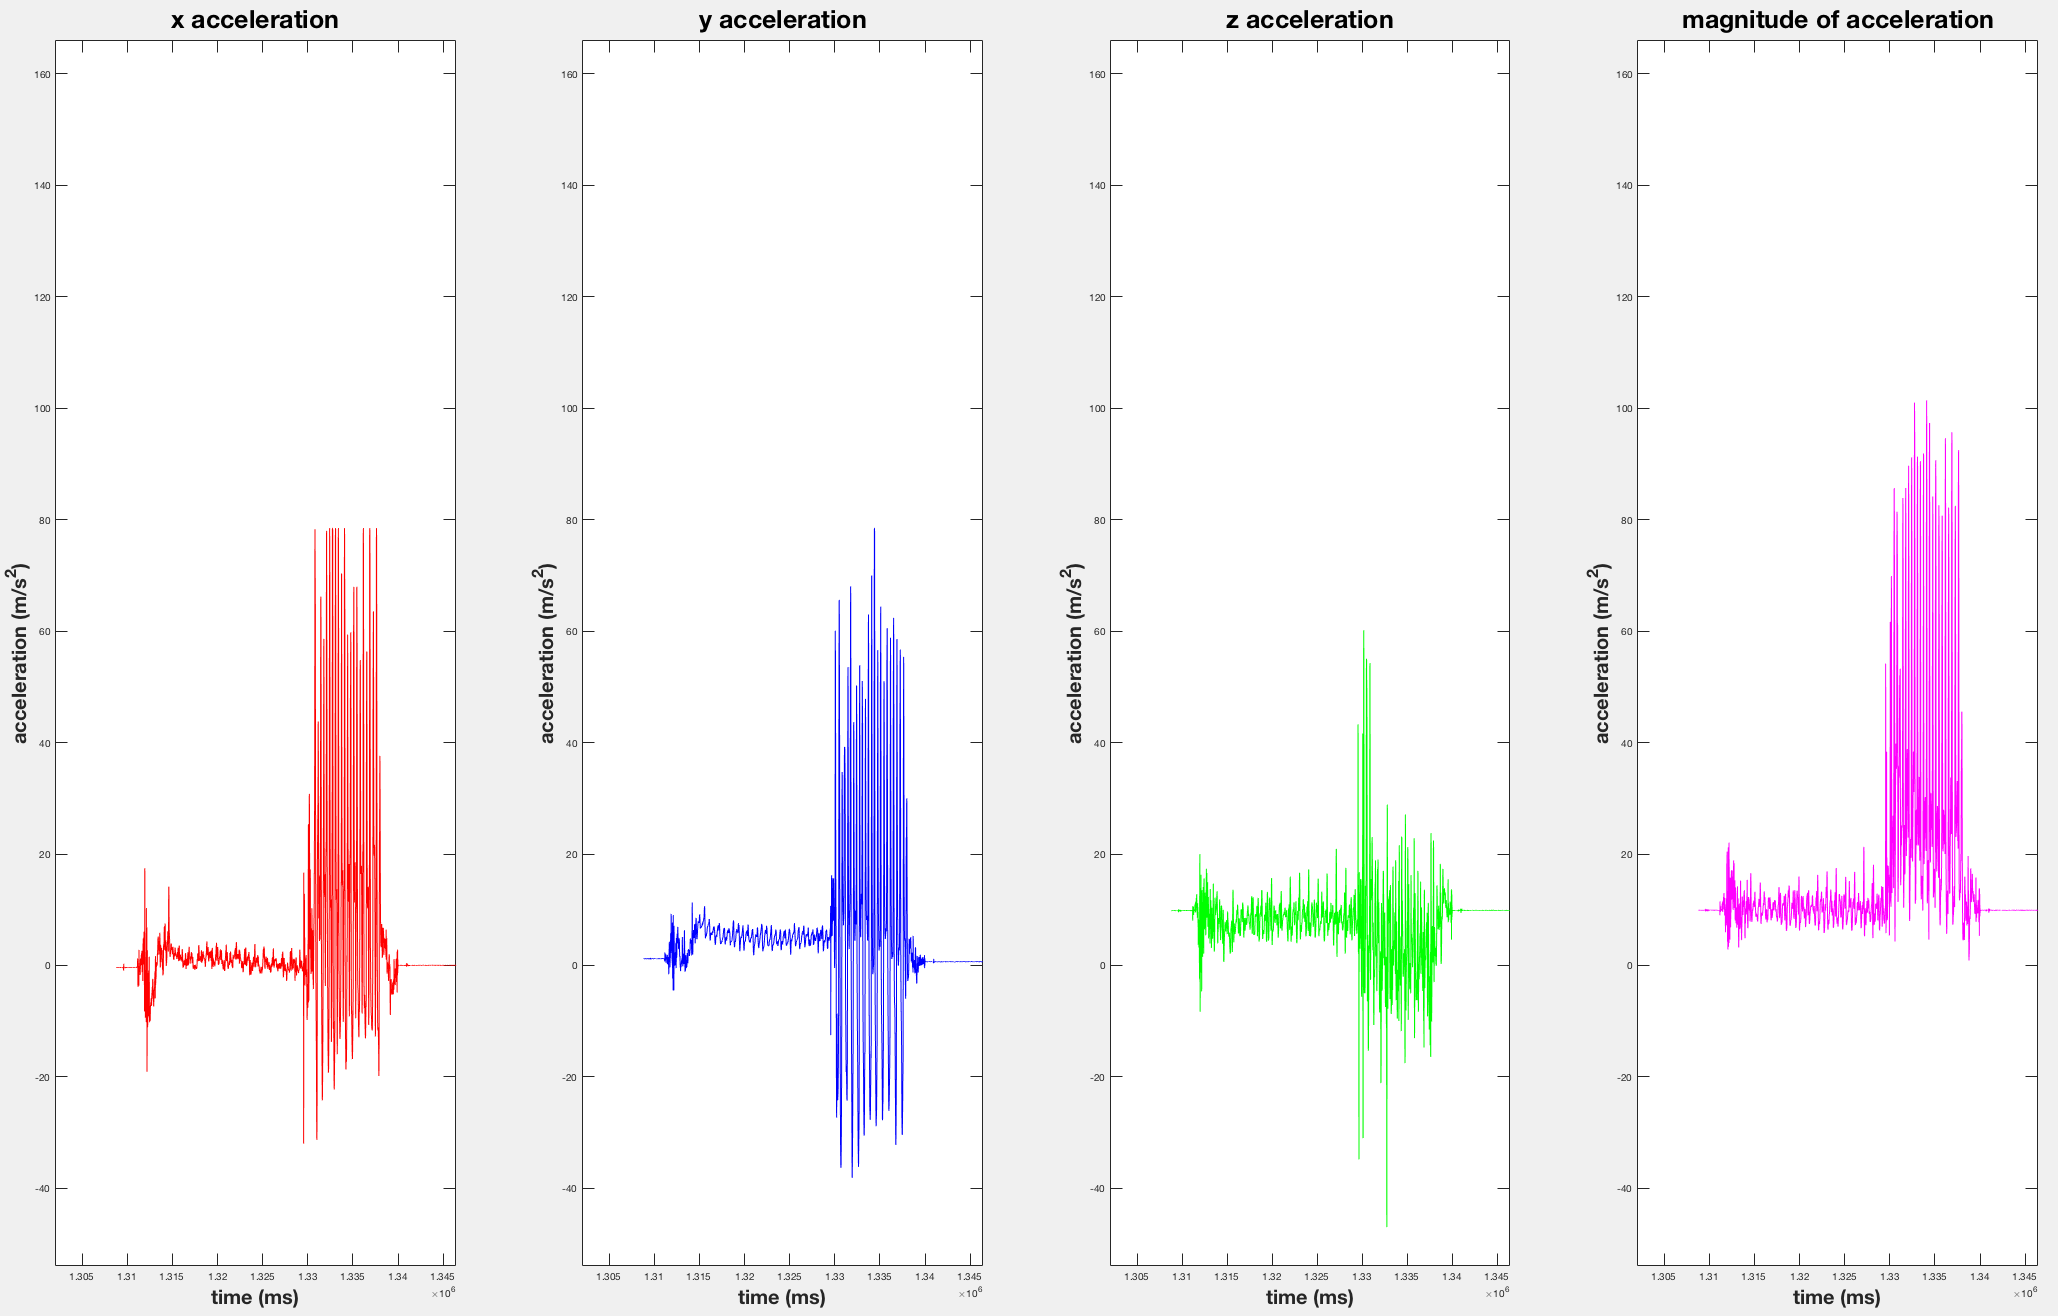
\includegraphics[width=1.0\columnwidth]{pos_acc_separated.png}
\caption{The X, Y, Z and magnitude of acceleration, respectively, from one simulated theft instance.}
\label{fig:simtheft}
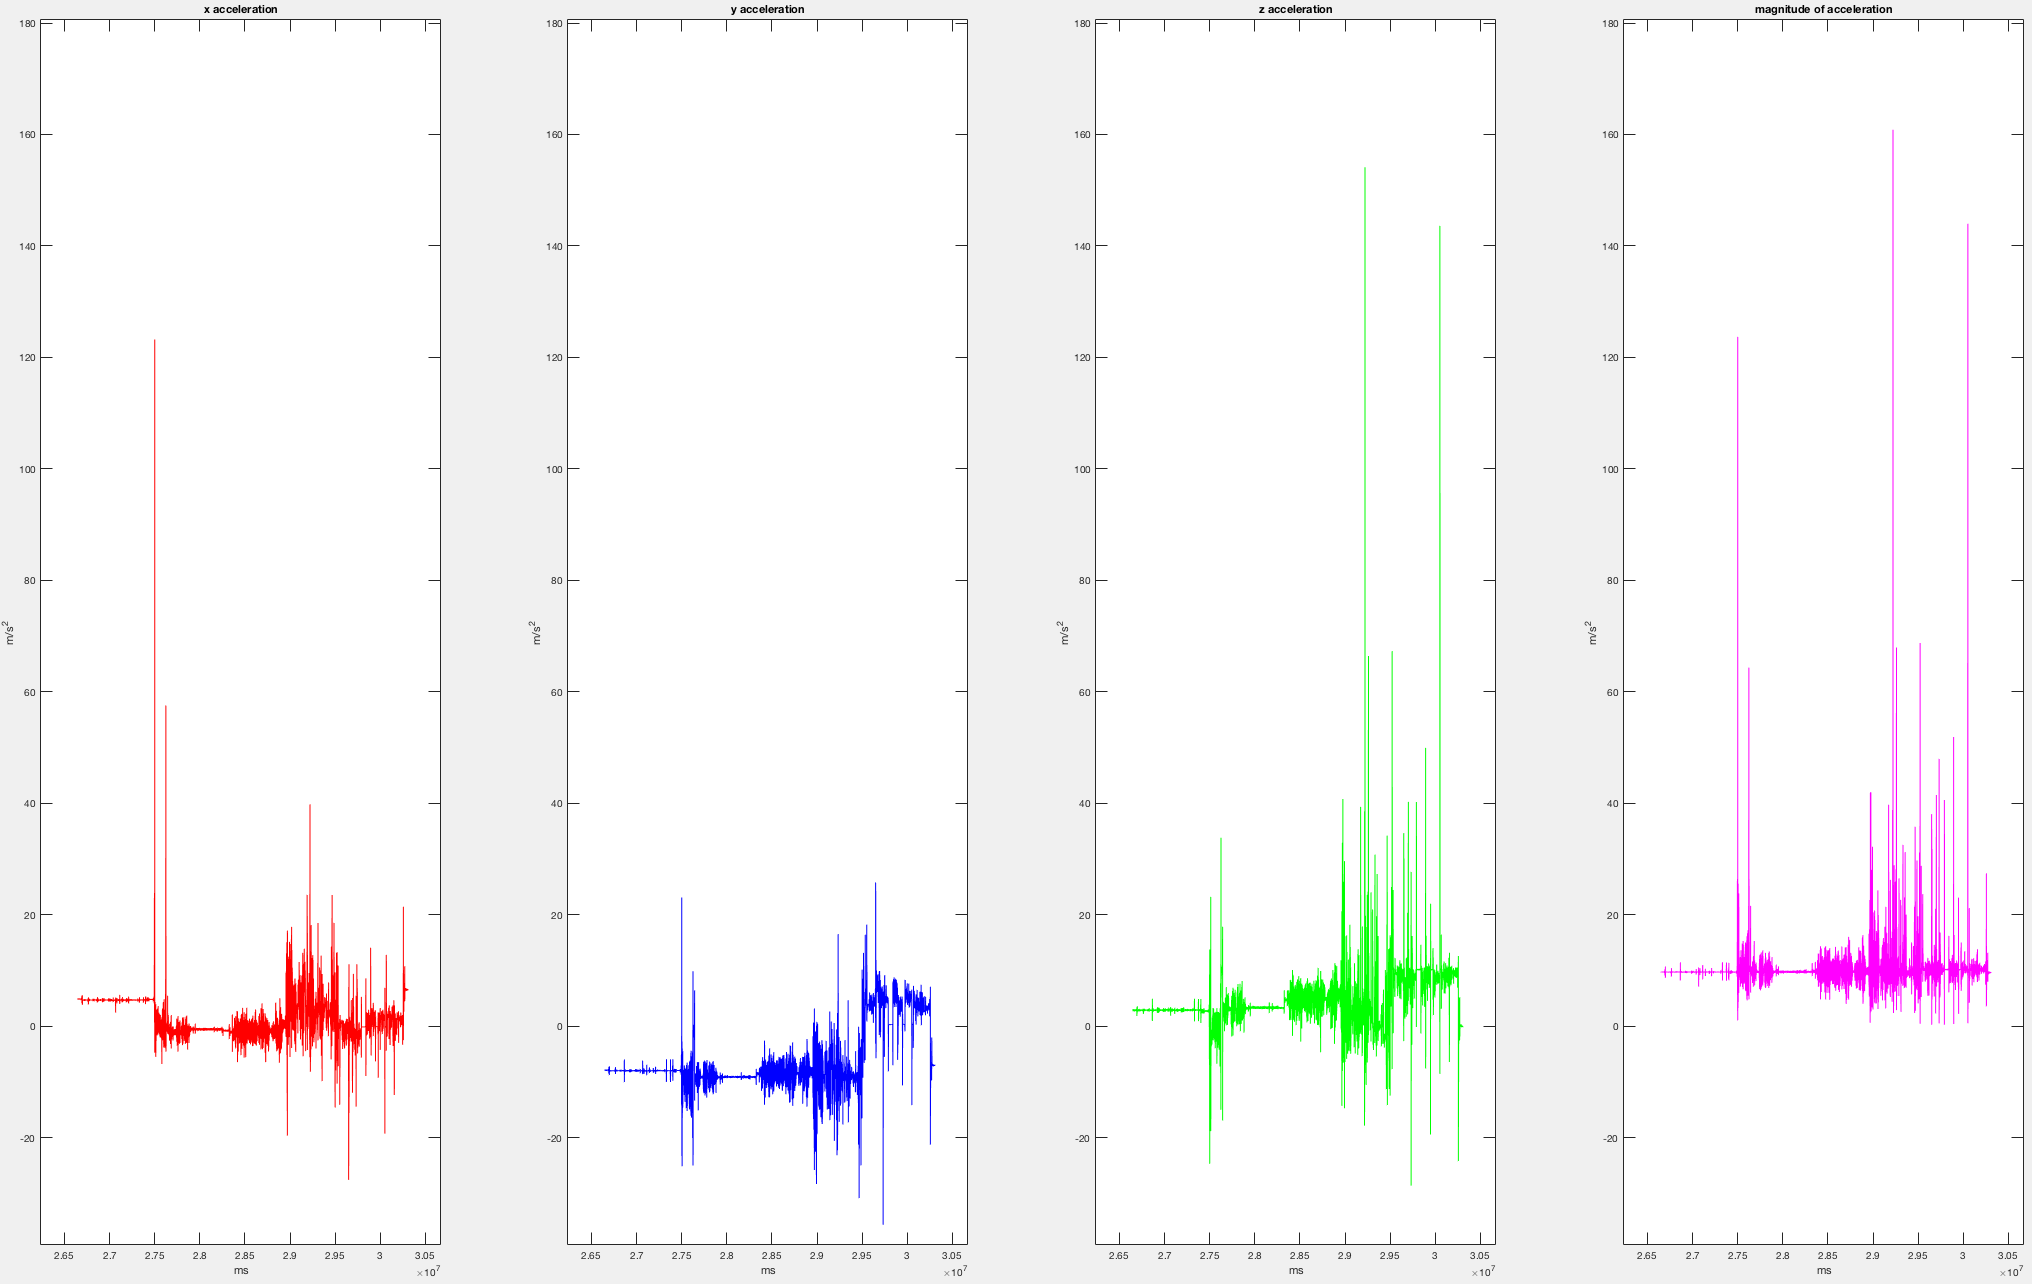
\includegraphics[width=1.0\columnwidth]{neg_acc_separated.png}
\caption{The X, Y, Z and magnitude of acceleration, respectively, during normal usage at an arbitrary time period.}
\end{figure}




\subsubsection{Field Study}
We performed a field study to gather data from ordinary smartphone users while they perform everyday activities, including walking, running, driving, possibly excercising, and anything else that occurred during their lives over the field study period.
% We obtained approval from the University of California, Berkeley IRB (Institutional Review Board) for this study. 
We obtained approval from our university IRB for this study. 
The study was conducted in a metropolitan area from September to December 2016.
% The study was conducted in the Bay Area of the United States from September to December 2016.
None of the participants experienced a phone theft during the study interval,
so we were able to use the accelerometer data collected from the user study as negative samples for our machine learning algorithms (i.e., instances of non-theft activity).

We posted a recruitment advertisement on Craigslist in September 2016. 
% We posted a recruitment advertisement on the Craigslist under the SF Bay Area `jobs et cetera' category in September 2016. 
We only recruited participants who used an Android smartphone with version 5.0 and above. 
After obtaining their consent, we installed our data collection application on their phones and collected data for a three-week period.
The application ran in the background and collected accelerometer sensor readings continuously, 24 hours a day.
We contacted participants weekly to make sure their phones were functioning correctly and troubleshoot any data collection issues.
Each participant was paid \$150 for their participation.

The study was divided across 3 rounds; each round lasted 3 consecutive weeks. 
A total of 55 participants were recruited, and
53 out of the 55 subjects completed the study. 
In the first round, 2 of the 18 participants did not complete the study.
Detailed demographic information about the participants of this user study is listed in Table~\ref{tbl:demographics}.
In aggregate, they used 21 different smartphone models from 6 different manufacturers and 8 different Adroid versions. This ensures the dataset containing diverse devices, and the classifiers are not specific to a particular type of smartphone or Adroid version.
We also asked participants how they typically carried their phone, when it was not in their hands; 33 reported keeping it in their pockets, 9 in their purses, 12 in multiple locations (e.g., pocket or purse, pocket or backpack), and 1 did not respond.
During the study, the subjects carried their phones while performing daily activities, for example walking, driving, running and possibly excercising. Data from a wide variety of real-world activities ensures the generability of the classifiers trained on it. 

\begin{table}[H]
\centering
\begin{tabular}{rrrrrr}
\hline
      & Male & Female & Age 20--29 & 30--39 & 40+ \\ \hline
R1    & 5    & 11     & 8         & 6     & 2   \\
R2    & 10   & 8      & 7         & 7     & 4   \\
R3    & 11   & 8      & 9         & 4     & 6   \\
Total & 26   & 27     & 24        & 17    & 12  \\ \hline
\end{tabular}
\caption{Participants' demographic information.}
\label{tbl:demographics}
\end{table}




\subsection{Feature Extraction}
\label{s:features}

Our theft scenarios all involved a sudden movement of the phone, which causes a large acceleration.
Therefore, as a first filtering step, we filtered the data to focus on times near when a large motion occurs.
In particular, our classifier is activated when the magnitude of acceleration $M$ exceeds~$40 m/s^2$.
We extract a one-second window before the activation time and a $n$-second window after the activation time, compute features on each of these windows, and use them for classification.
We vary $n$ from 1 to 7 to obtain the best classification accuracy.
We chose a threshold of~$40 m/s^2$ as all of our simulated thefts experienced accelerations exceeding that threshold when the phone was initially grabbed by the thief.

We first identified 16 candidate features, 8 features for each of the two windows.
In particular, we computed the minimum, maximum, mean, standard deviation, root mean square, arc length, product of arc length and standard deviation, and mean absolute value, each computed on the magnitude values ($M$) within the window.
We chose to only compute these features on the magnitude of the acceleration, and not the $X$, $Y$, and $Z$ components, because the magnitude is non-directional and thus more robust to changes in the orientation of the phone. 
We then visualized the distribution of these features for the two classes and applied feature selection techniques to choose a subset of features that yield good performance.
We removed the minimum and mean absolute value from the feature list because removing them did not affect the performance of the classifiers. 
As a result, we extract a 12-dimensional feature vector, 6 features from the before-window and 6 from the after-window, every time the detector is triggered.

Let $M_1,\dots,M_k$ denote the time series of acceleration magnitudes within the window.
The features are computed as follows:
\begin{itemize}
\item \emph{Maximum}: the maximum value of the magnitude within the window, i.e., $\max(M_1,\dots,M_k)$.
\item \emph{Mean}: the average value of magnitude in a window, i.e., $(M_1+\dots + M_k)/k$.
\item \emph{Standard deviation}: the standard deviation of magnitude values in a window.
\item \emph{Root mean square}: the RMS of magnitude values in a window, i.e., $(M_1^2 + \dots + M_k^2)^{1/2}/k^{1/2}$.
\item \emph{Arc length}: the average of the absolute differences between all adjacent magnitude values in a window, i.e., $(|M_2-M_1| + |M_3-M_2| + \dots + |M_k-M_{k-1}|)/(k-1)$.
Intuitively, this captures the average of the first derivative of the acceleration.
\item \emph{Product of arc length and standard deviation}: the product of the two feature values.
\end{itemize}

Because the accelerometer sensor reports readings in the same units on all Android phones, and because our features are relatively simple, we believe these features capture fundamental, device-independent characteristics of the motion rather than anything specific to the particular device used for data capture (e.g., in contrast to the hardware-based differences documented by Dey et al.~\cite{Dey2014}).

We obtained 60 positive instances from the 60 simulated thefts.
After applying the~$40 m/s^2$ threshold, we obtained approximately approximately 248,000 negative samples from the data collected in the field study. 
We then applied boolean classification techniques to this data set.


% \begin{figure}[t]
% 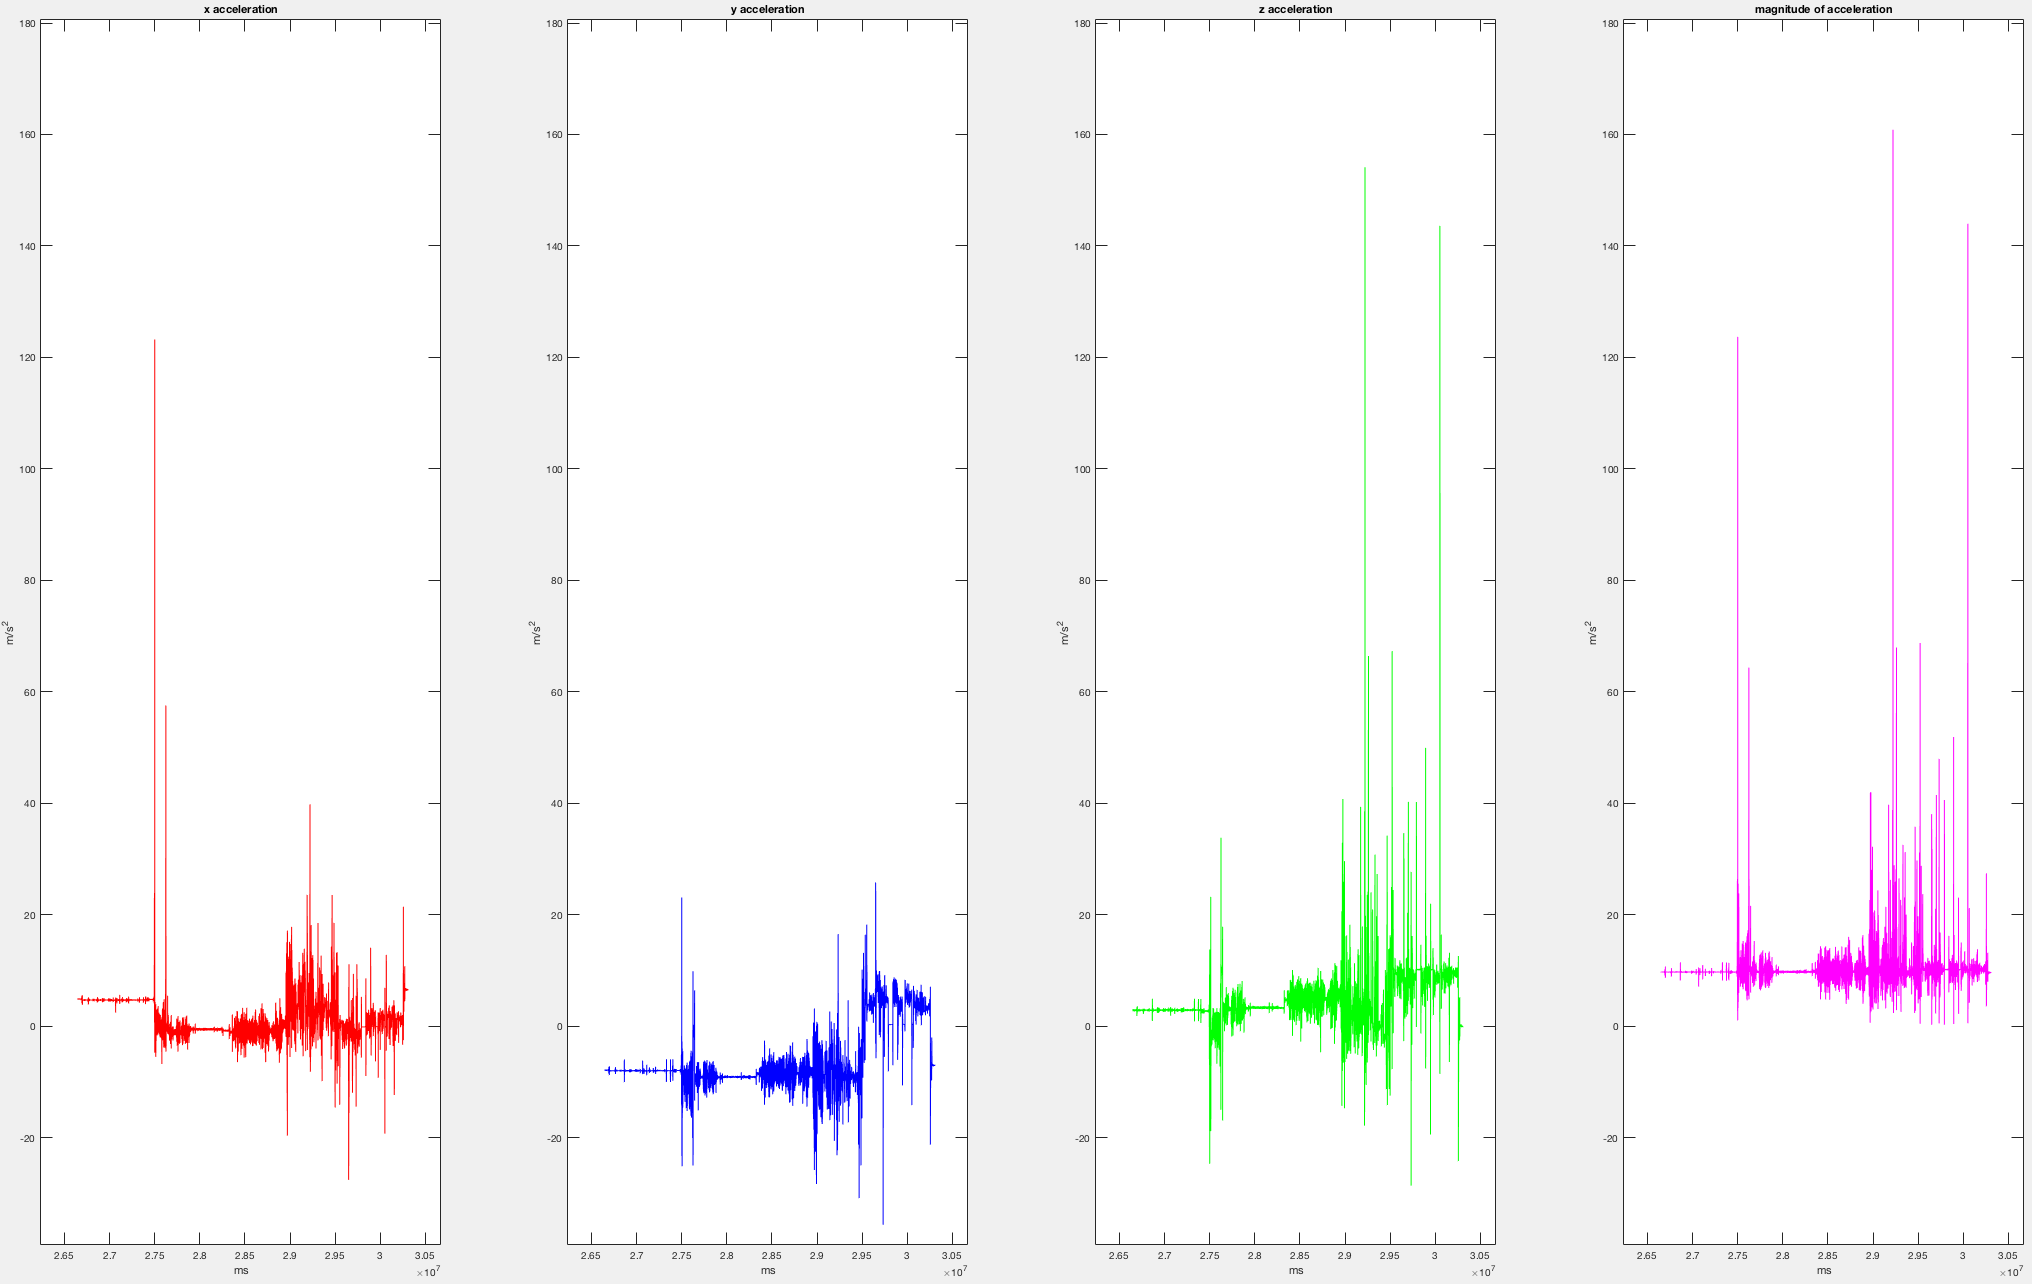
\includegraphics[width=1.0\columnwidth]{neg_acc_separated.png}
% \caption{The X, Y, Z and magnitude of acceleration, respectively, during normal usage at an arbitrary time period.}
% \end{figure}



\subsection{Machine Learning Algorithms}
We evaluate three standard machine learning algorithms: linear SVM, logistic regression and random forests.
Because we have many more negative samples than positive ones, we tried different settings for class weights to weight positive instances more highly than negative ones.
We also evaluated different window sizes for the after-window.
We found that a 2-second after-window yielded better accuracy than a 1-second after-window since 2-second windows encapsulate more complete acceleration information about the motions, and larger window sizes did not offer much improvement.
Therefore, all of our experiments use a 1-second before-window and a 2-second after-window.
We partitioned the entire dataset, which consists of 120 positive samples and approximately 248,000 negative samples, into training and test sets with 7:3 ratio.
Then we trained the classifiers on the training set and reported the predition results of the test set.



\section{Results}
Among the three classifiers, logistic regression performs the best.
Confusion matrices for logistic regression, random forests, and a linear SVM
are shown in Table~\ref{fig:cmat}.
The logistic regression classifier has a false positive rate of 0.09\%. Given that the field study involved 53*3=159 person-week of data, and the logistis regression would report 248,000*0.09\%=223 false positives, the total number of samples extracted from the field study data times the false positive rate. This means that on average users receive 223/159$\approx$1.4 false alarm every week, and a true positive rate of 100\%.
The random forests classifier has an even lower false positive rate (approximately one false alarm per month),
but it only detects 60\% of the thefts.

Only a small fraction of predicted positives will actually be theft, but we expect this will be acceptable due to the relatively low cost of false positives: it means users will have to unlock their phones one extra time per week, which seems likely to be tolerable. We report the false positive rate rather than precision, because the false positive rate is easily interpretable and not sensitive to the rate at which theft occurs. The precision is sensitive to the number of simulated thefts included in the dataset, which might not match the number of actual thefts that are likely to occur over a given period of time.


\begin{table}[t]
\centering
\begin{tabular}{@{}lll@{}}
\toprule
              & Predicted Negative & Predicted Positive \\ \midrule
True Negative & 74446              & 72                 \\
True Positive & 0                  & 37                 \\ \bottomrule
\end{tabular}

\begin{tabular}{@{}lll@{}}
\toprule
              & Predicted Negative & Predicted Positive \\ \midrule
True Negative & 74503              & 15                 \\
True Positive & 14                 & 23                 \\ \bottomrule
\end{tabular}

\begin{tabular}{@{}lll@{}}
\toprule
              & Predicted Negative & Predicted Positive \\ \midrule
True Negative & 74501              & 17               \\
True Positive & 17                 & 20                 \\ \bottomrule
\end{tabular}
\caption{Confusion matrices for a logistic regression classifier (at top; with class weights 1:200), random forests classifier (middle; class weights 1:5000), and a linear SVM classifier (bottom; class weights 1:1000).}
\label{fig:cmat}
\end{table}

% \begin{table}[t]
% \centering
% \begin{tabular}{@{}lll@{}}
% \toprule
%               & Predicted Negative & Predicted Positive \\ \midrule
% True Negative & 248223             & 170                \\
% True Positive & 0                  & 60                 \\ \bottomrule
% \end{tabular}
% \caption{Confusion matrix for a logistic regression classifier trained
% with class weights set to 1:200.}
% \label{fig:logistic}
% \end{table}

% \begin{table}[t]
% \centering
% \begin{tabular}{@{}lll@{}}
% \toprule
%               & Predicted Negative & Predicted Positive \\ \midrule
% True Negative & 248360             & 33                 \\
% True Positive & 32                 & 28                 \\ \bottomrule
% \end{tabular}
% \caption{Confusion matrix for a random forests classifier trained with
% class weights set to 1:5000.}
% \label{fig:rf}

% \end{table}

% \begin{table}[t]
% \centering
% \begin{tabular}{@{}lll@{}}
% \toprule
%               & Predicted Negative & Predicted Positive \\ \midrule
% True Negative & 246522             & 1871               \\
% True Positive & 42                 & 18                 \\ \bottomrule
% \end{tabular}
% \caption{Confusion matrix for a linear SVM classifier trained with
% class weights set to 1:1000.}
% \label{fig:svm}
% \end{table}


To get a better understanding of why our classifier is successful,
we computed feature rankings to find the most predictive features.
For logistic regression, we used standardized coefficients as the feature importance score:
the score for feature $i$ is $|\alpha_i| \cdot \sigma_i$, where $\alpha_i$ is the coefficient for feature $i$ in the logistic regression model and $\sigma_i$ is the standard deviation of feature $i$ in the training set.
In addition, we computed the 95\% confidence intervals for all standardized coefficents using 50 epoches of the entire data set.
The feature importance scores and their 95\% confidence intervals for the logistic regression classifier are listed in Table~\ref{tbl:importance-lr}.
The most discriminative features are
the maximum of the before-window,
the product of arc length and standard deviation of the after-window,
and the arc length of the before-window.
Plotting a histogram of feature values (see Figures~\ref{fig:beforehist} and \ref{fig:afterhist}), we can see that those features do appear to provide good discrimination.


\begin{table}[t]
\centering
\begin{tabular}{@{}ll@{}}
\toprule
Feature                & Feature Importance \\ \midrule
Root mean square (b)   &   143.8786849  ($\pm$ 0.08714717)       \\
Mean (b)               &   129.8910092 ($\pm$ 0.08033373)       \\ 
Root mean square (a)   &  \ 93.8382532  ($\pm$ 0.04439512)       \\
Mean (a)               &  \ 88.1273891  ($\pm$ 0.03972303)       \\
Standard deviation (a) &  \ 66.7204655  ($\pm$ 0.02228971)       \\
Standard deviation (b) &  \ 47.7685313  ($\pm$ 0.03349549)       \\
Arc length (a)         &  \ 27.3736785  ($\pm$ 0.01463394)       \\
Maximum (b)            & \ \ 2.73231469 ($\pm$ 0.00041407)       \\
Arc length * SD (a)    & \ \ 2.69875036 ($\pm$ 0.00097762)       \\
Arc length (b)         & \ \ 1.16578948 ($\pm$ 0.00855526)       \\
Maximum (a)            & \ \ 0.05985700 ($\pm$ 0.00065551)       \\
Arc length * SD (b)    & \ \ 0.04950325 ($\pm$ 0.00090281)       \\ \bottomrule

\end{tabular}
\caption{Feature importances and their 95\% confidence intervals for logistic regression. (b) denotes the features extracted from the 1s window before the 40-spike; (a) denotes the features extracted from the 2s window after the 40-spike.}
\label{tbl:importance-lr}
\end{table}

We also rank the features for the random forests classifier using scikit-learn's feature importance score, which estimates the relative importance of the features by computing the expected fraction of the samples they contribute to. 
Thus the higher in the tree, the more important the feature is~\cite{sklearn:rfdoc}. 
% 0.04751106, 0.0080411, 0.02881483, 0.01533719, 0.02245781, 0.03309431, 0.12388036, 0.20288397, 0.16426152, 0.21908845, 0.05162059, 0.0830088.
We also computed the 95\% confidence intervals for all feature importance scores using 50 epoches of the entire data set.
The resulting feature importance scores and their 95\% confidence intervals for the random forests classifier are listed in Table~\ref{tbl:importance-rf}.

% Another way to visulize the representative features is to plot a histogram of dataset and to see which features can better seperate the positive and negative data points, as shown in Figures 1 and 2.

\begin{table}[t]
\centering
\begin{tabular}{@{}ll@{}}
\toprule
Feature                & Feature Importance \\ \midrule
Root mean square (a)   & 0.24251892 ($\pm$ 0.00734018)         \\
Mean (a)               & 0.19351276 ($\pm$ 0.00685086)         \\
Standard deviation (a) & 0.17634030 ($\pm$ 0.00601571)         \\
Maximum (a)            & 0.10975278 ($\pm$ 0.00480411)         \\
Arc length * SD (a)    & 0.07541471 ($\pm$ 0.00382659)         \\
Arc length (a)         & 0.04821400 ($\pm$ 0.00264303)         \\
Maximum (b)            & 0.04740376 ($\pm$ 0.00172894)         \\
Arc length * SD (b)    & 0.03291854 ($\pm$ 0.00128944)         \\
Standard deviation (b) & 0.02828350 ($\pm$ 0.00115971)         \\
Arc length (b)         & 0.02072662 ($\pm$ 0.00103551)         \\
Root mean square (b)   & 0.01544474 ($\pm$ 0.00078121)         \\
Mean (b)               & 0.00946937 ($\pm$ 0.00077147)          \\ \bottomrule
\end{tabular}
\caption{Feature importances and their 95\% confidence intervals for random forests. (b) denotes the features extracted from the 1s window before the 40-spike; (a) denotes the features extracted from the 2s window after the 40-spike.}
\label{tbl:importance-rf}
\end{table}


% \begin{figure*}[t]

% \begin{center}
% \begin{minipage}
% 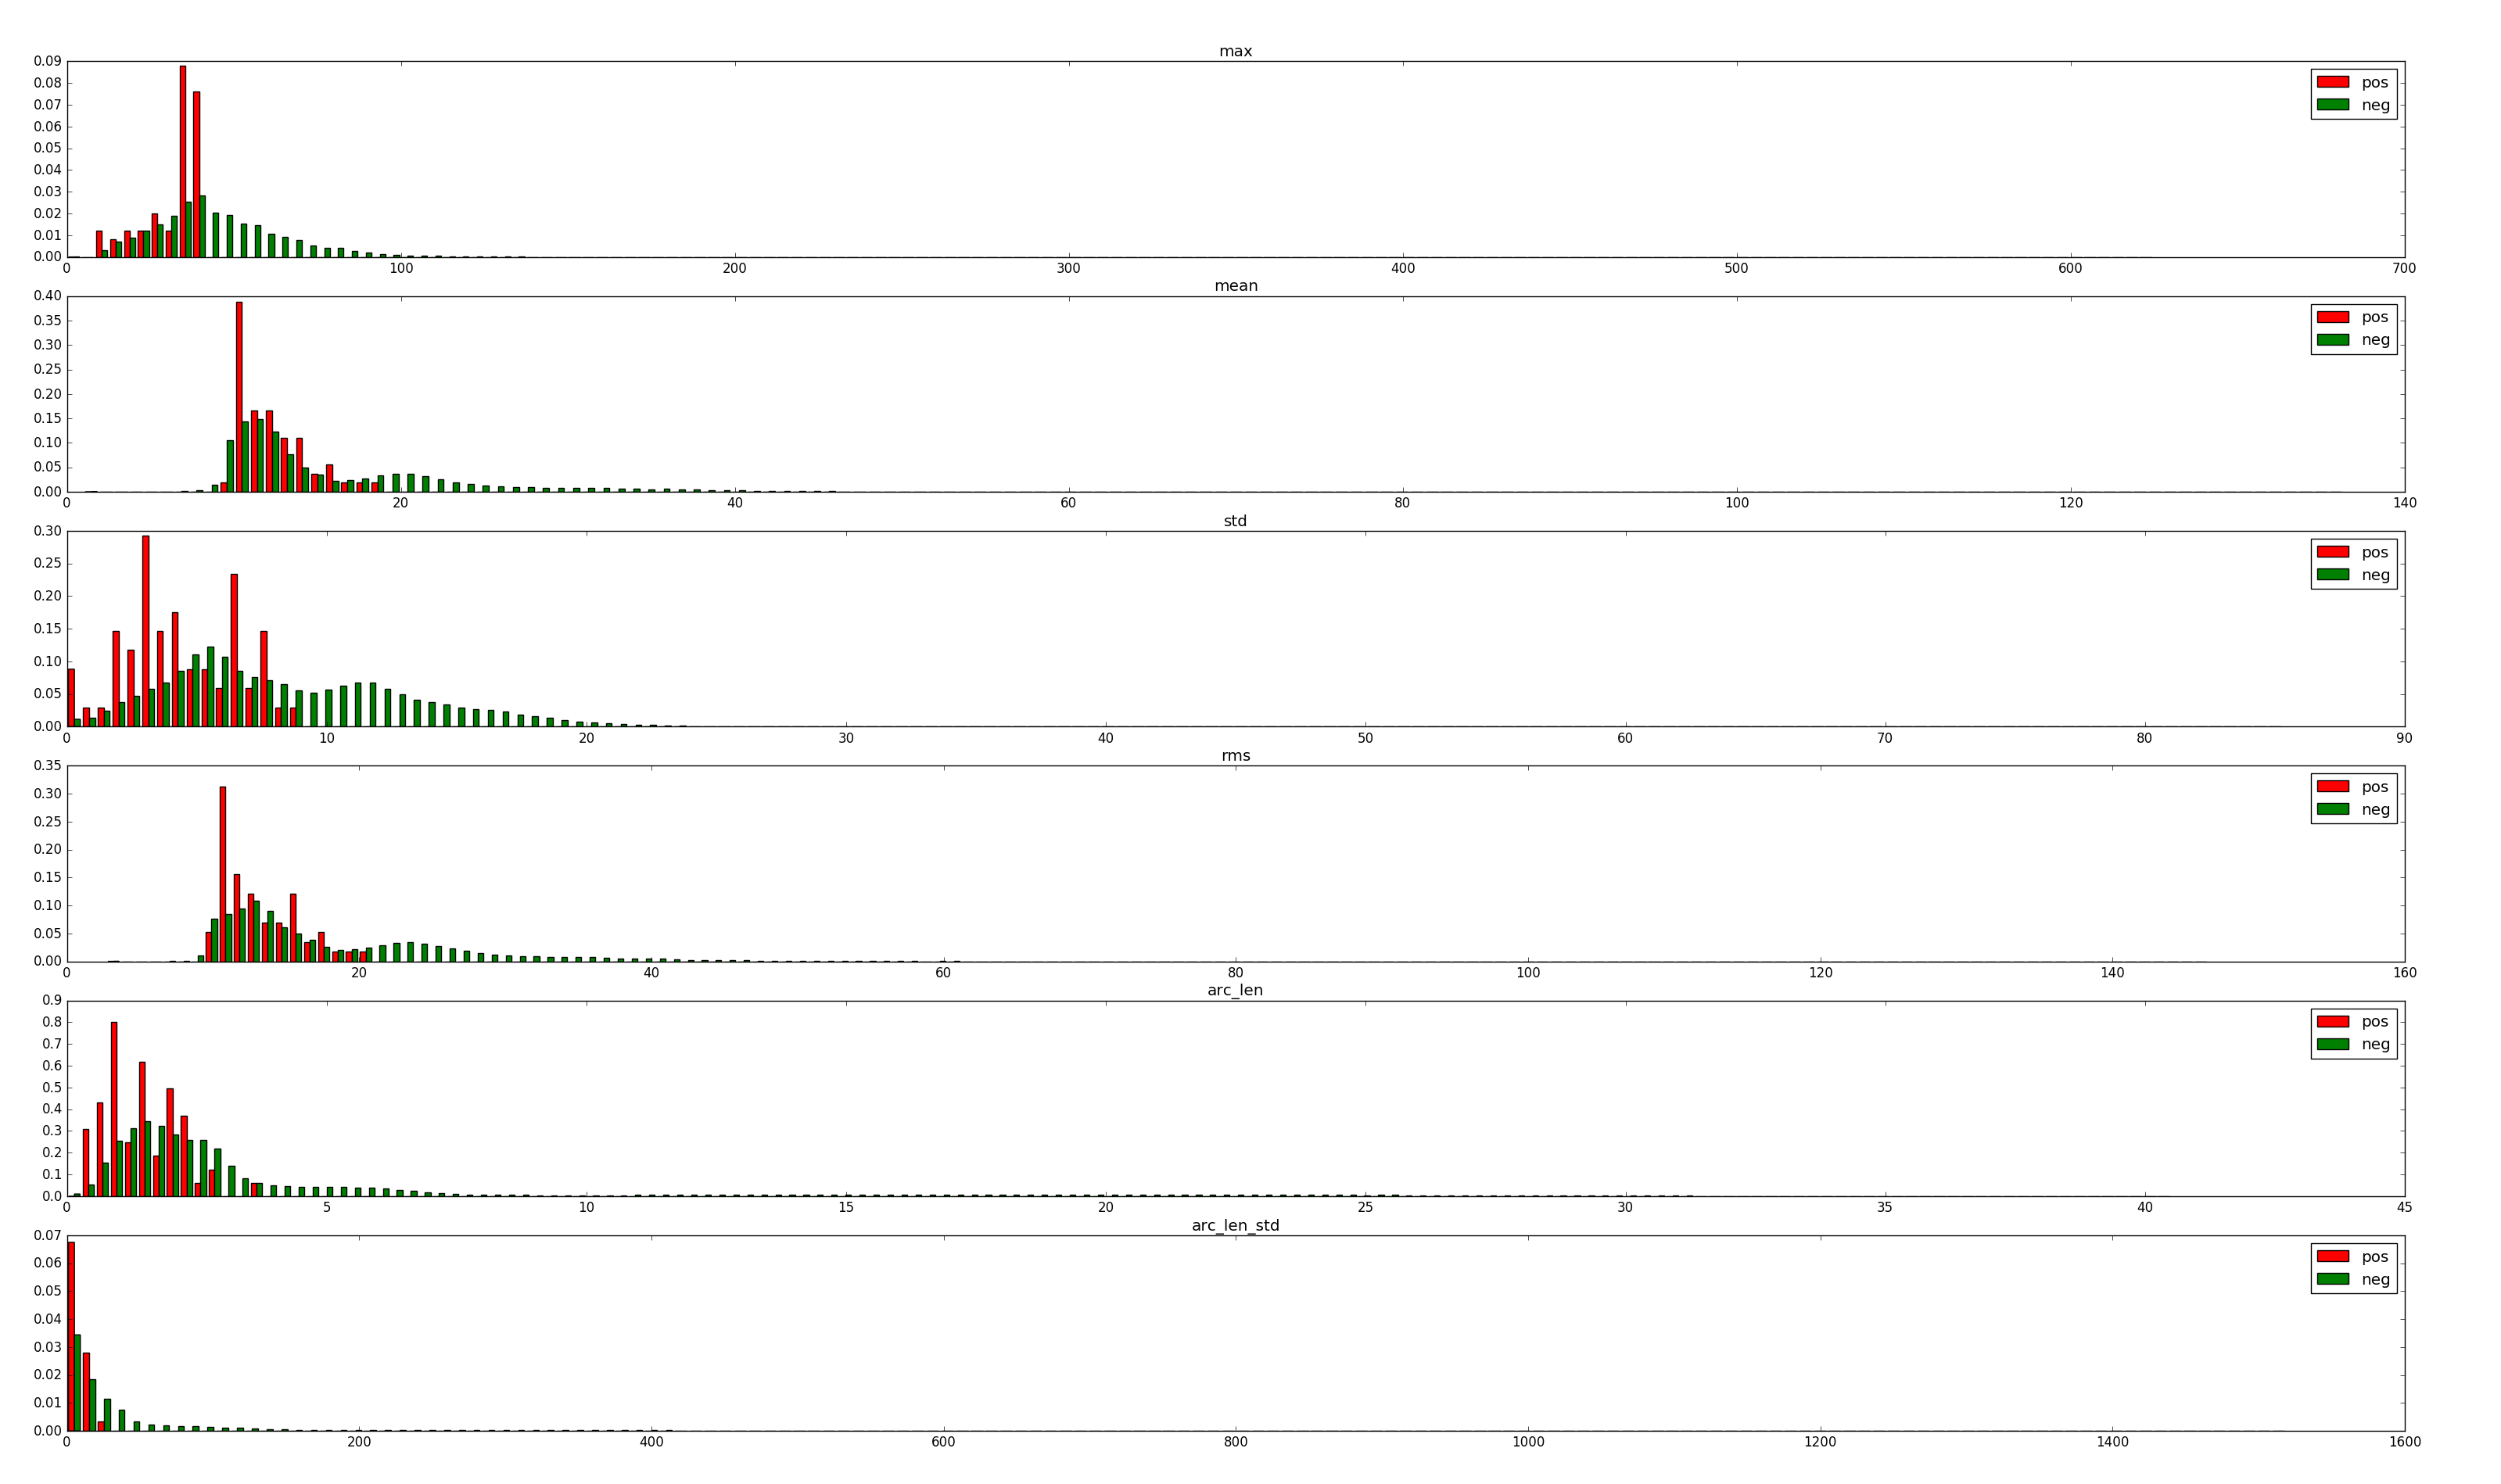
\includegraphics[width=\textwidth]{hist_features_before_win_size_1_2.png}
% \end{minipage}
% \end{center}
% \caption{Histogram for each of the 6 features for the 1-second window before the~$40 m/s^2$ spike.  The features are listed in the order presented in Section~\ref{s:features}, e.g., the top histogram is for the maximum.  Red bars indicate thefts, and green bars indicate non-theft windows.}
% \label{fig:beforehist}
% \begin{center}
% \begin{minipage}
% 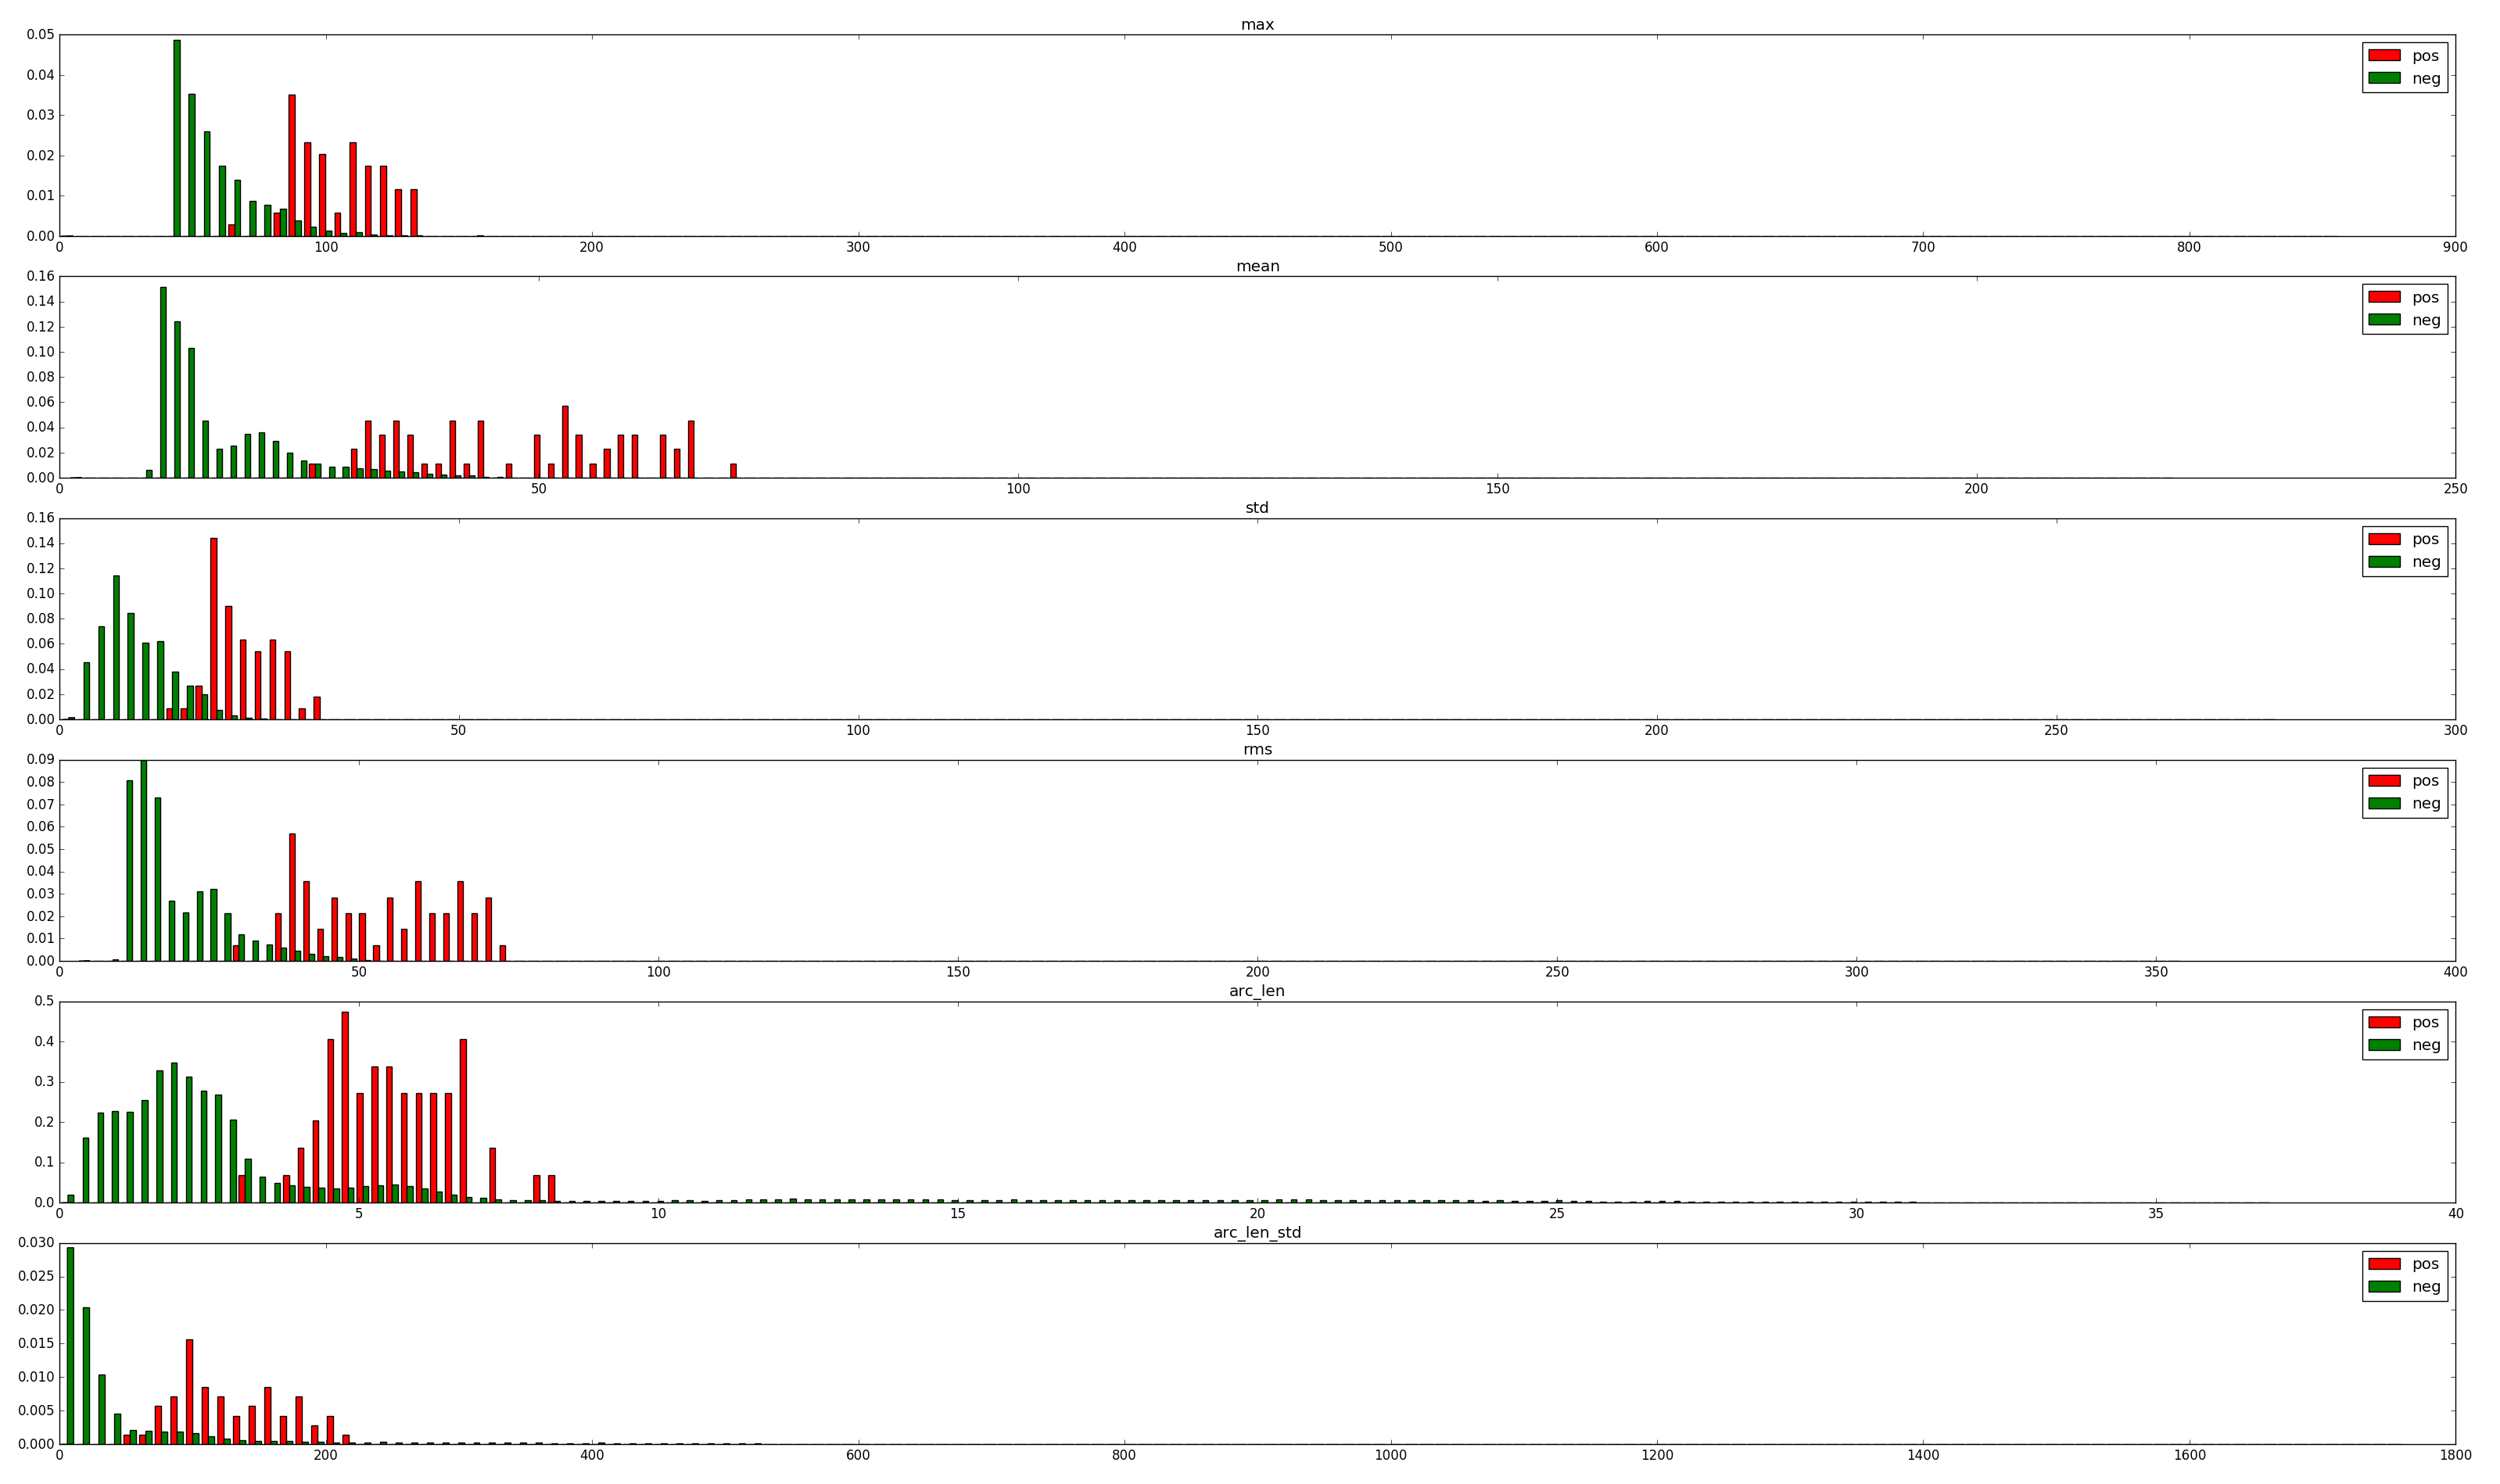
\includegraphics[width=\textwidth]{hist_features_after_win_size_1_2.png}
% \end{minipage}
% \end{center}
% \caption{Histogram of feature values in the 2-second window after the~$40 m/s^2$ spike.}
% \label{fig:afterhist}

% \end{figure*}


\begin{figure*}[t]
\centering
\begin{minipage}[t]{\columnwidth}
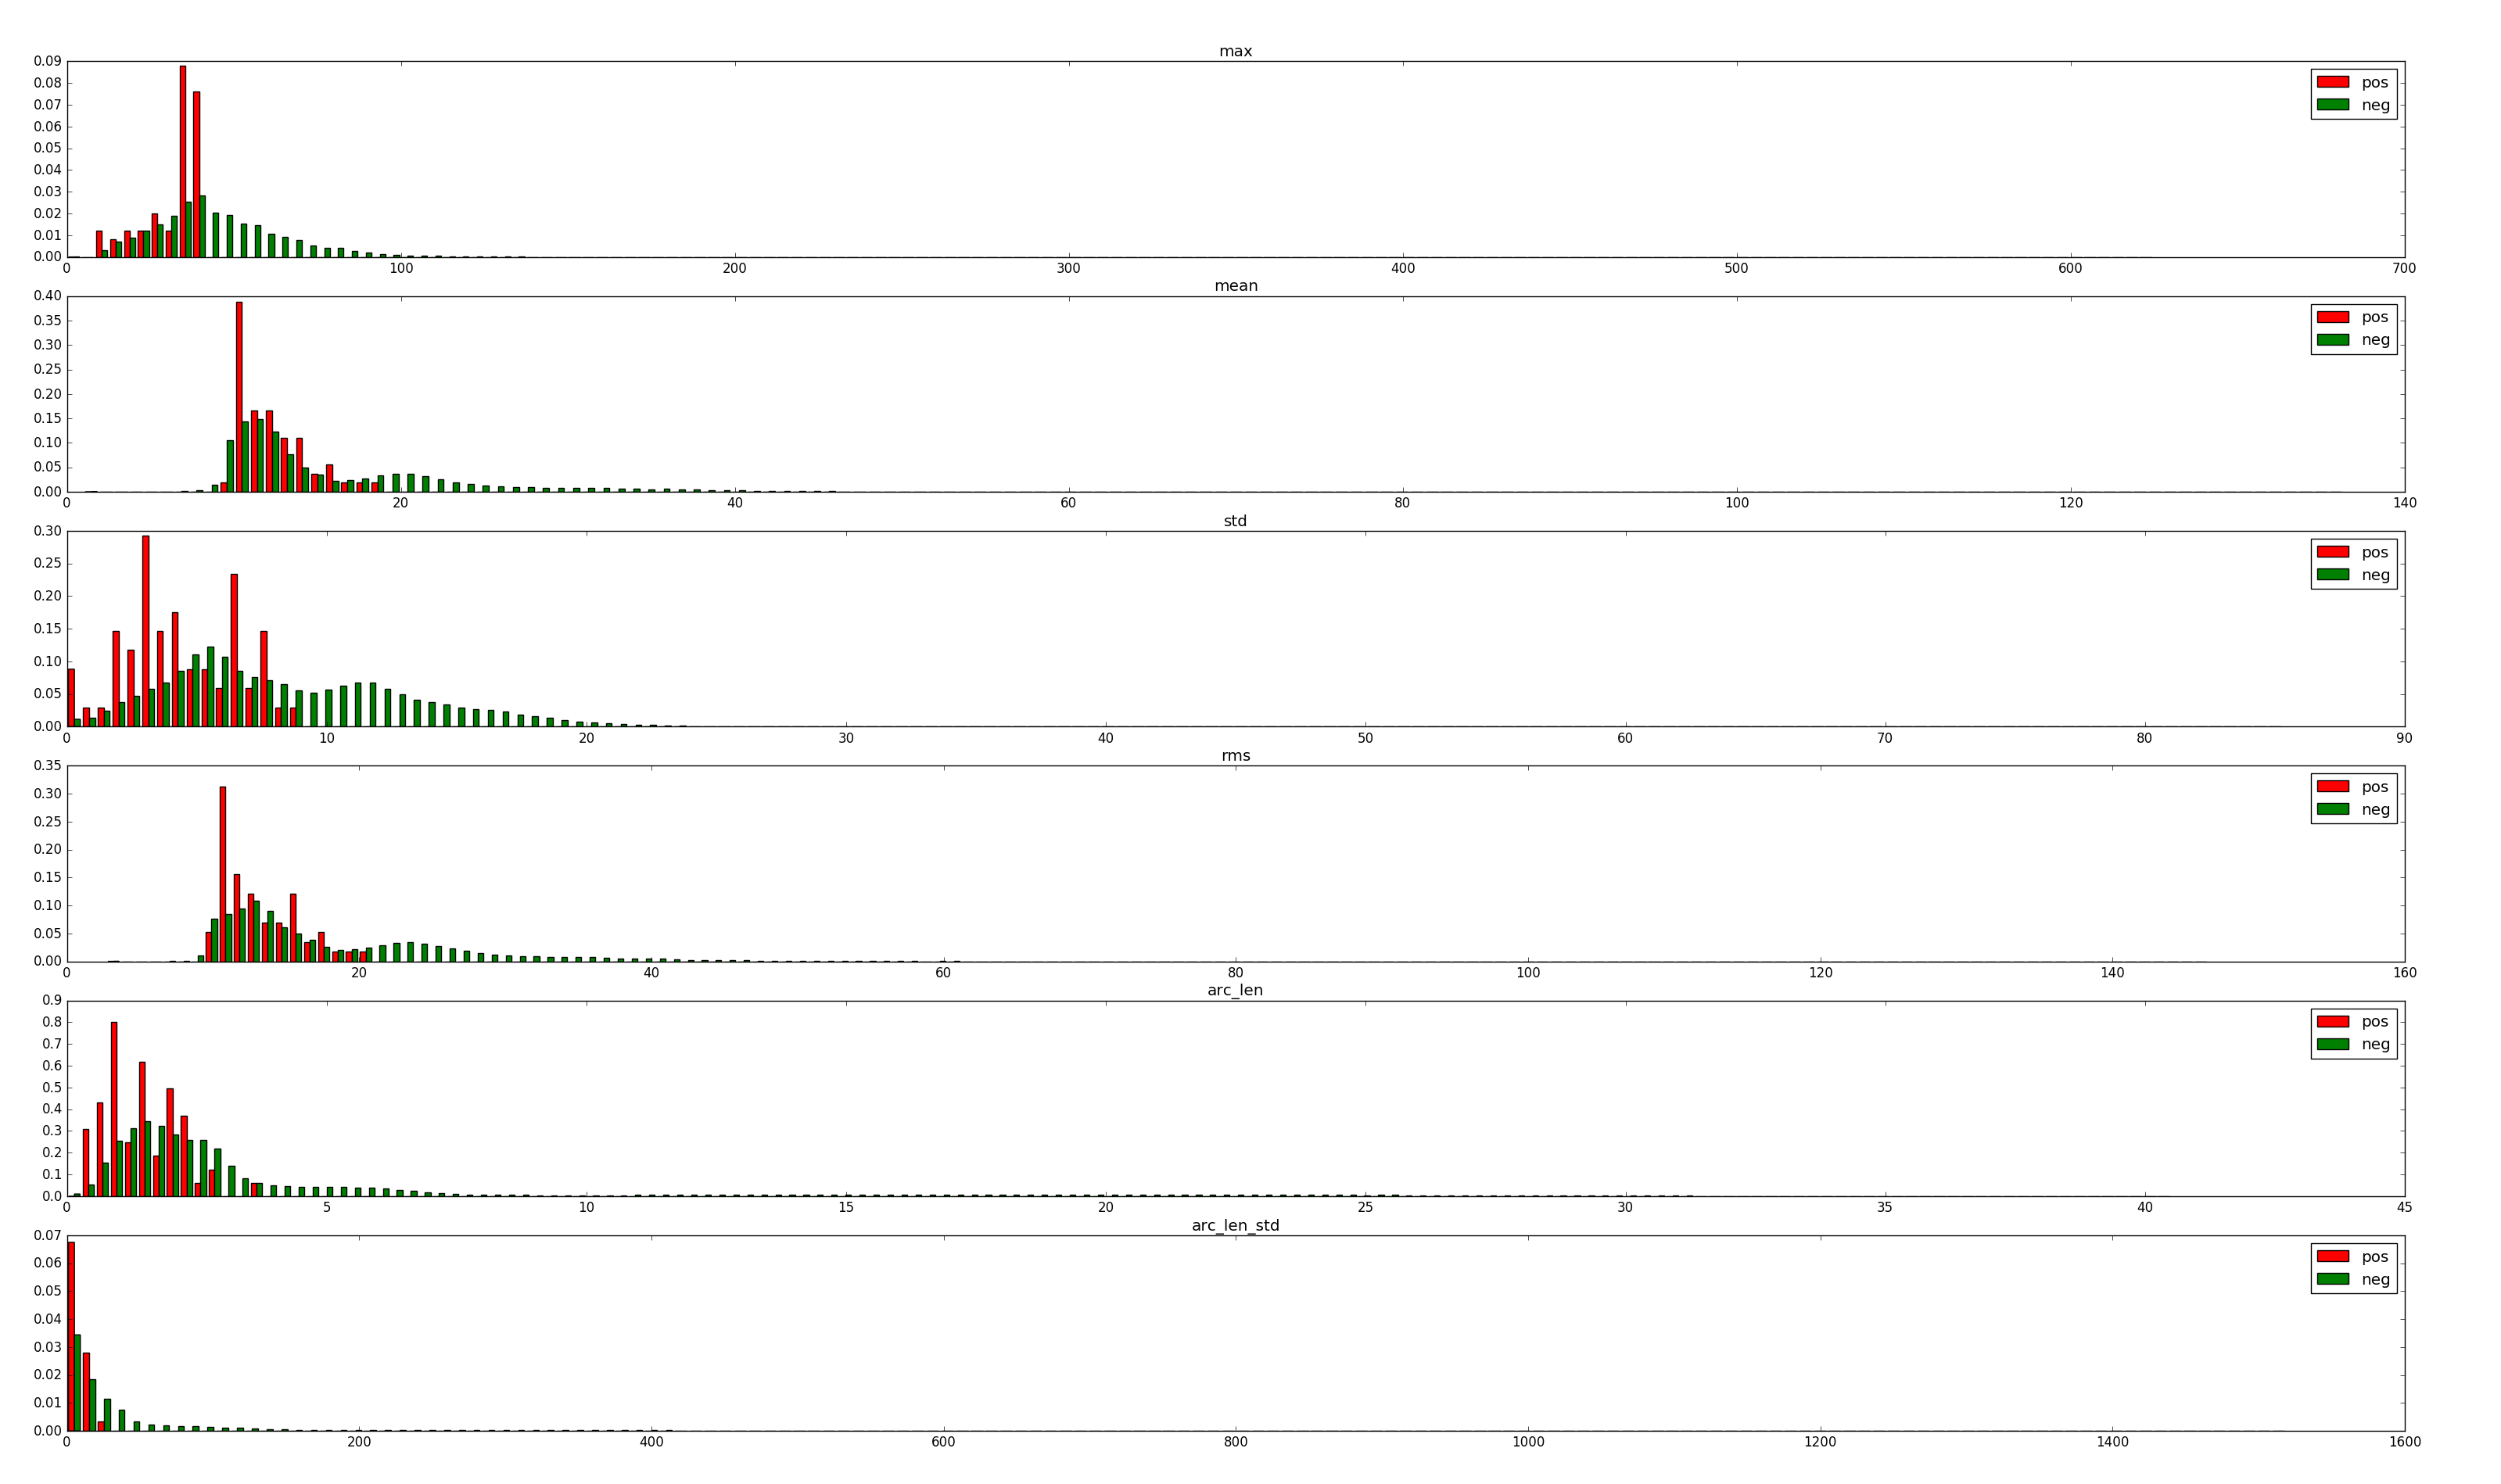
\includegraphics[width=\columnwidth]{hist_features_before_win_size_1_2.png}
\caption{Histogram for each of the 6 features for the 1-second window before the~$40 m/s^2$ spike.  The features are listed in the order presented in Section~\ref{s:features}, e.g., the top histogram is for the maximum.  Red bars indicate thefts, and green bars indicate non-theft windows.}
\label{fig:beforehist}
\end{minipage}
\hfill
\begin{minipage}[t]{\columnwidth}
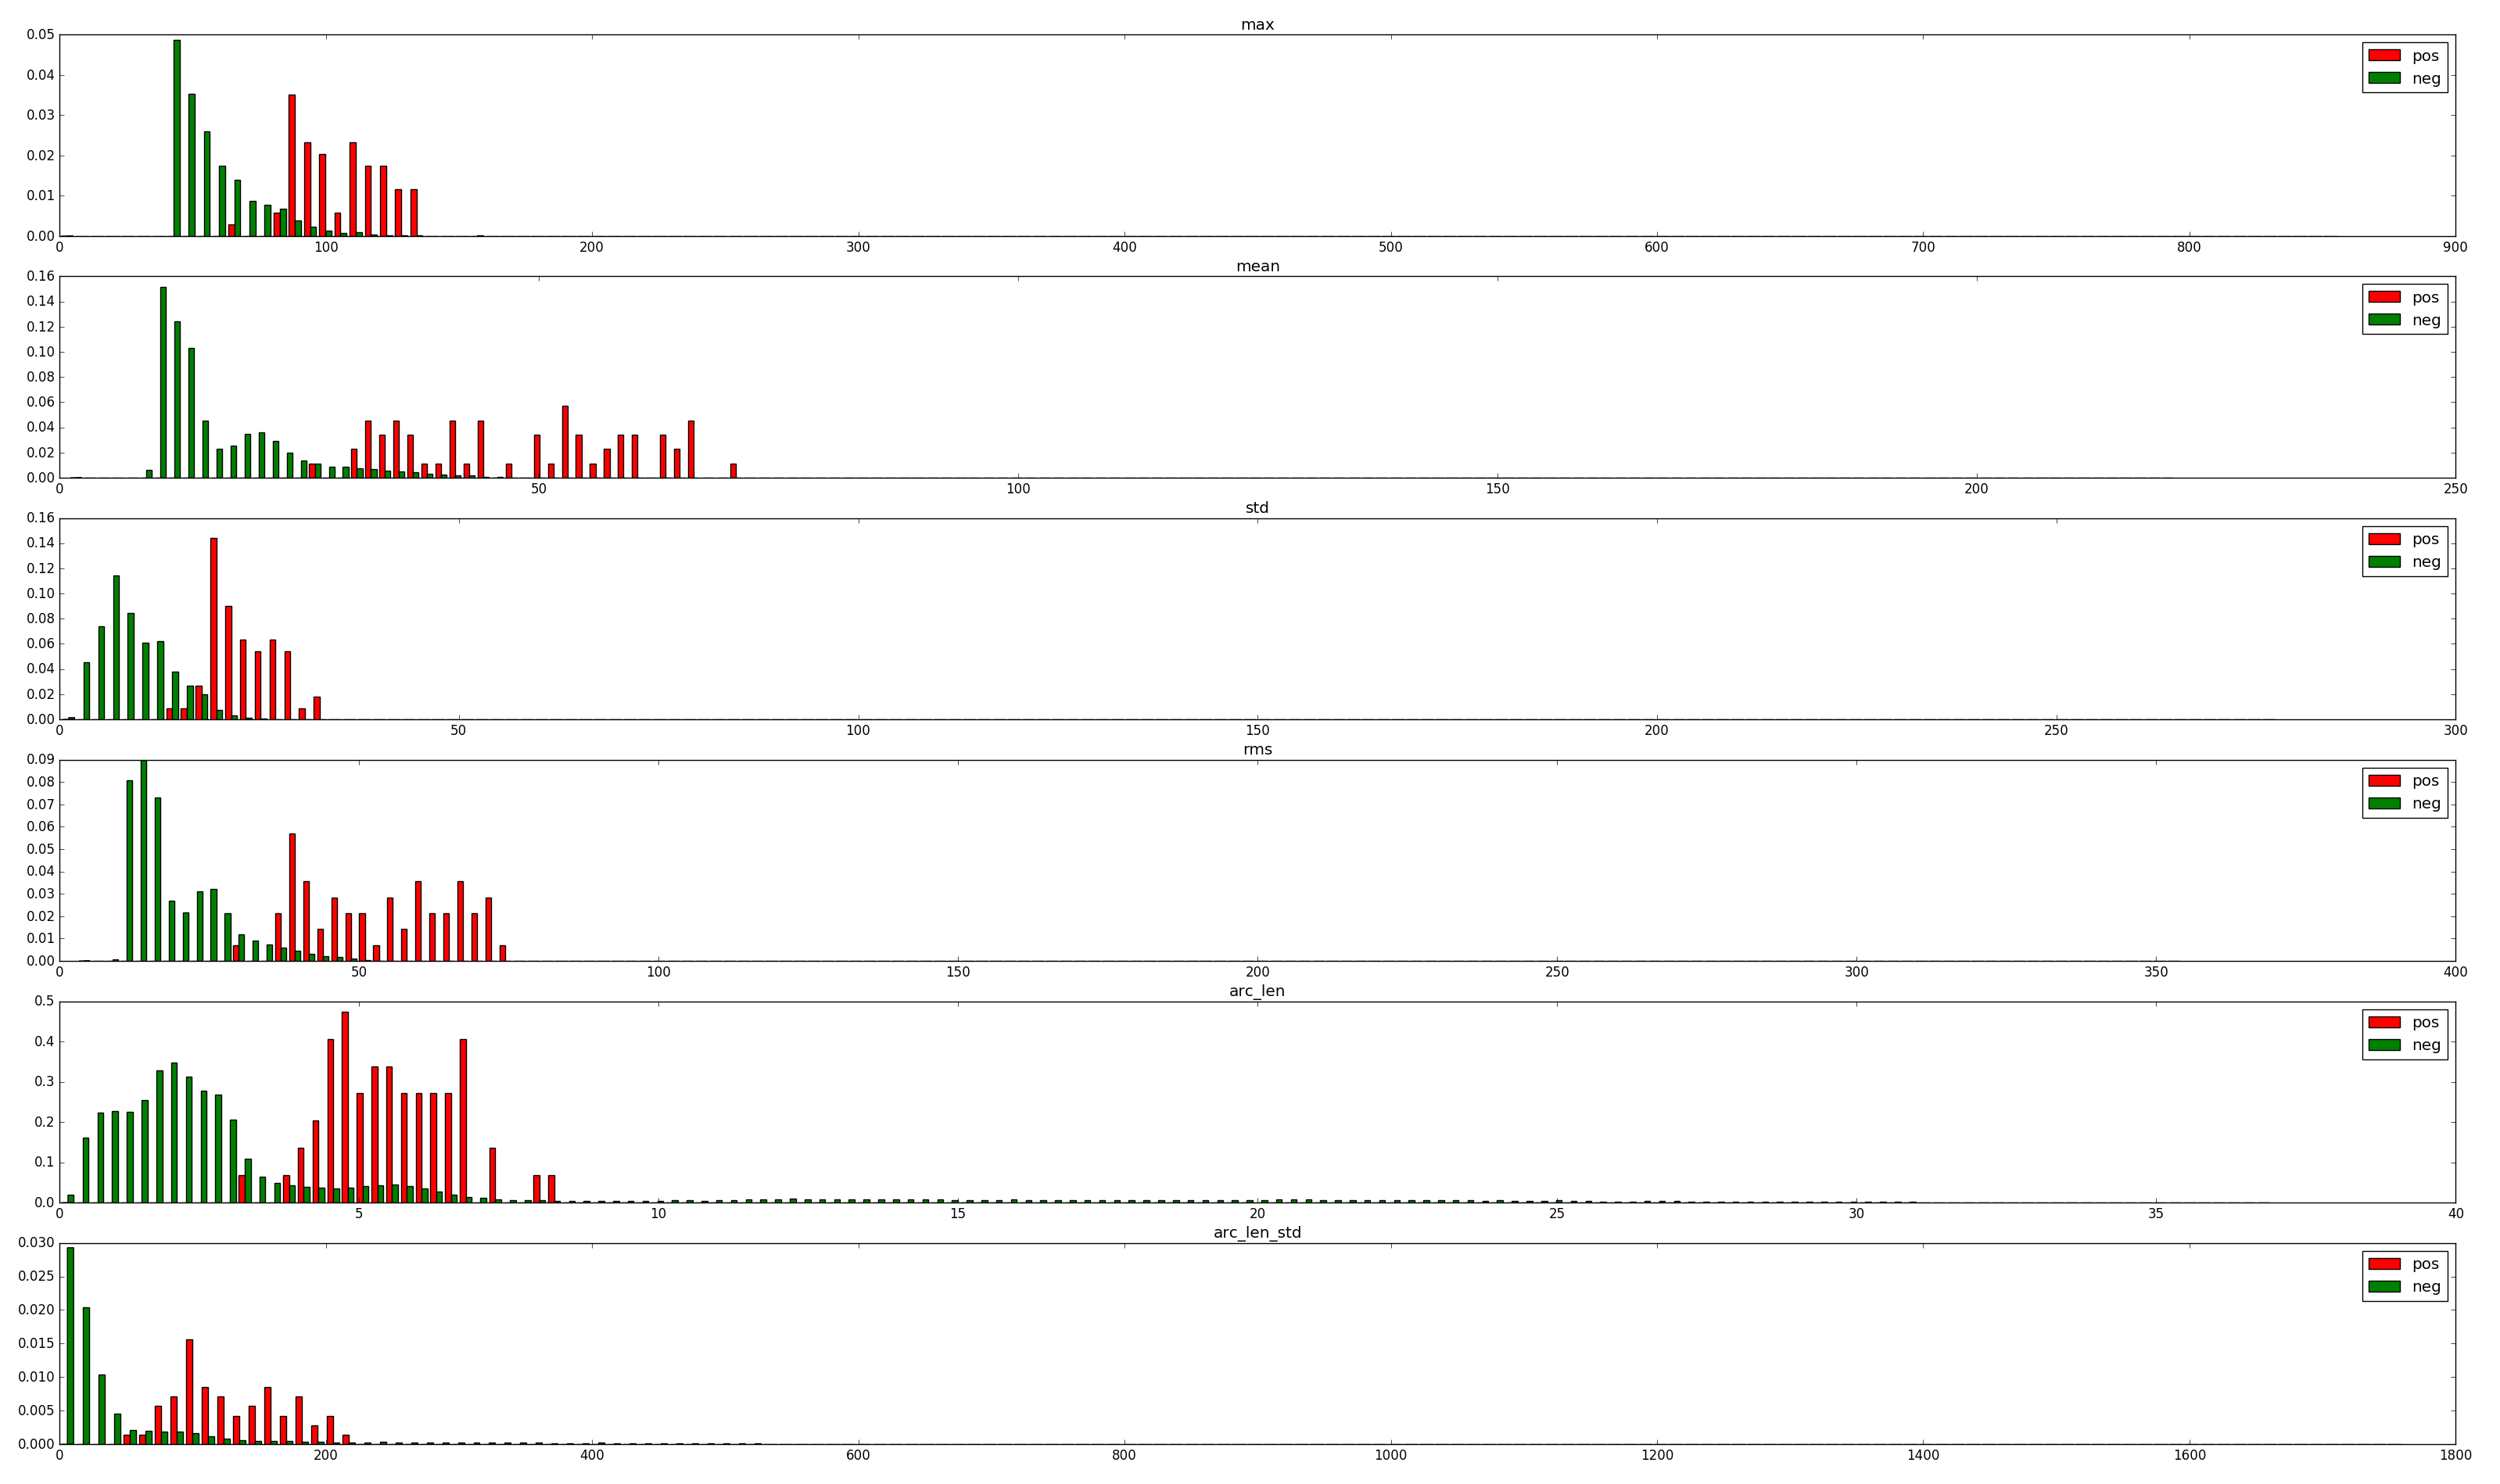
\includegraphics[width=\columnwidth]{hist_features_after_win_size_1_2.png}
\caption{Histogram of feature values in the 2-second window after the~$40 m/s^2$ spike.}
\label{fig:afterhist}
\end{minipage}
\end{figure*}

% \begin{figure*}[t]
% \begin{center}
% 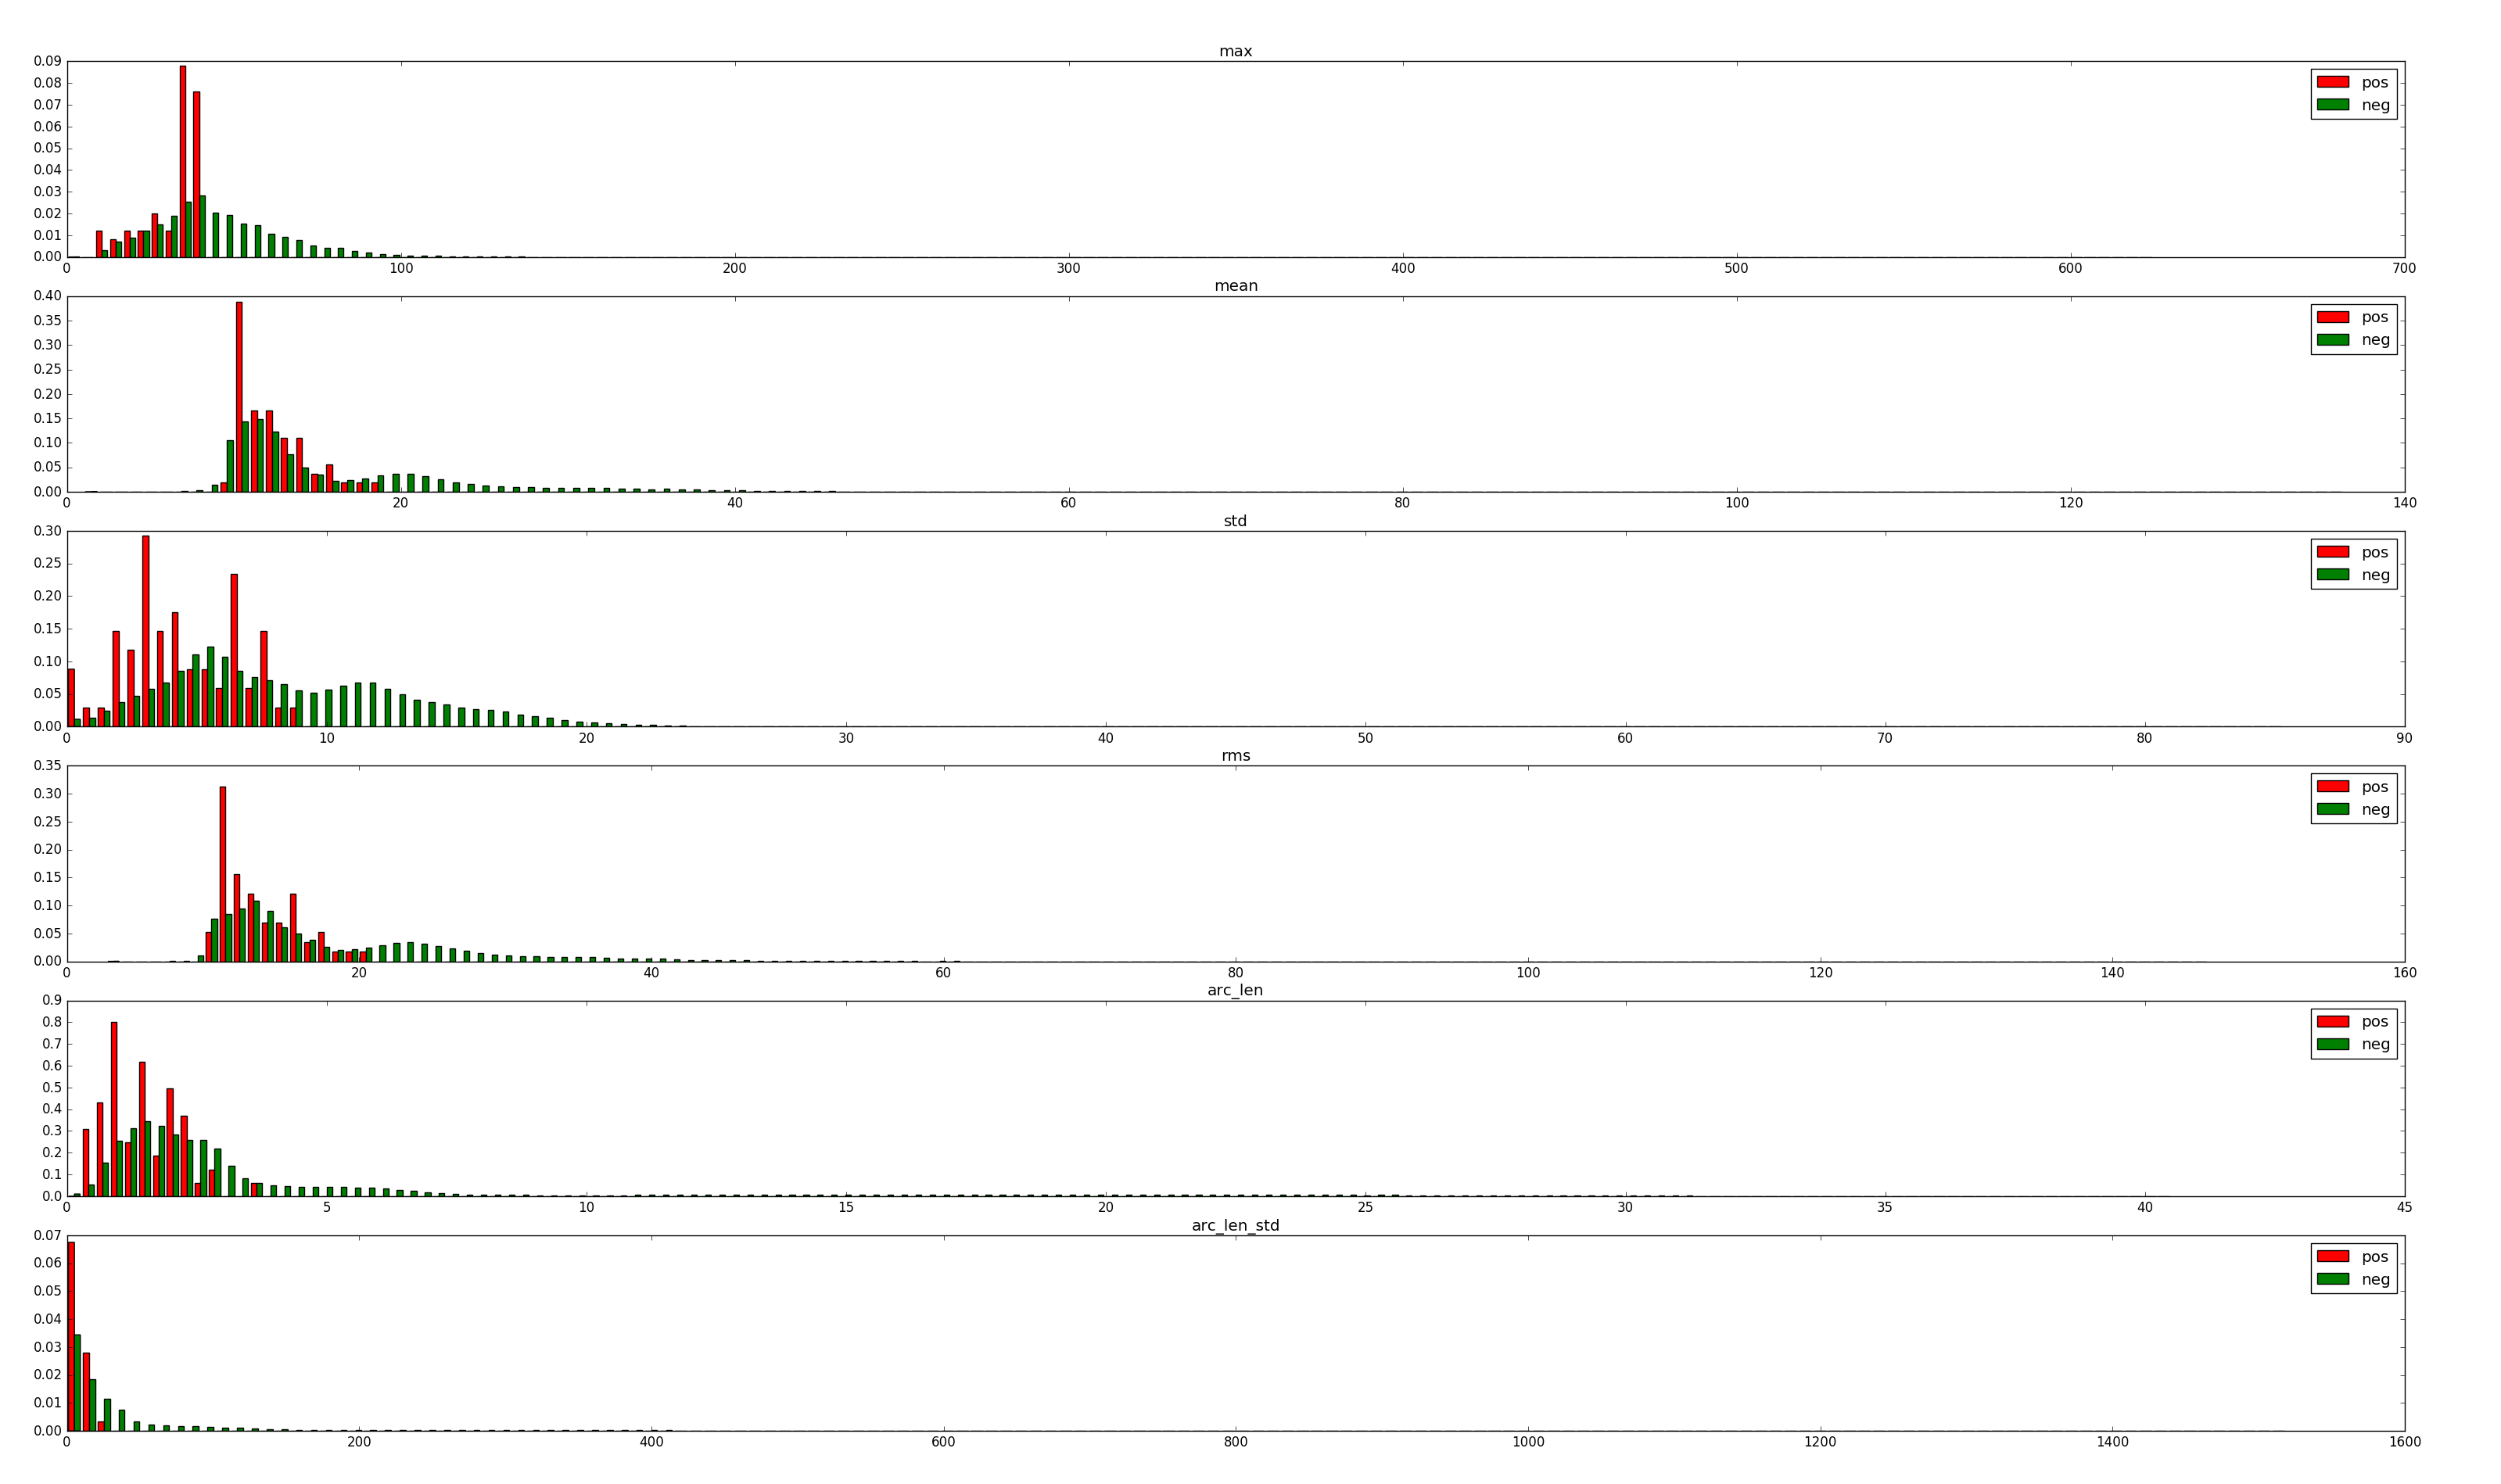
\includegraphics[width=\textwidth]{hist_features_before_win_size_1_2.png}
% \end{center}
% \caption{Histogram for each of the 6 features for the 1-second window before the~$40 m/s^2$ spike.  The features are listed in the order presented in Section~\ref{s:features}, e.g., the top histogram is for the maximum.  Red bars indicate thefts, and green bars indicate non-theft windows.}
% \label{fig:beforehist}
% \end{figure*}

% \begin{figure*}[t]
% \begin{center}
% 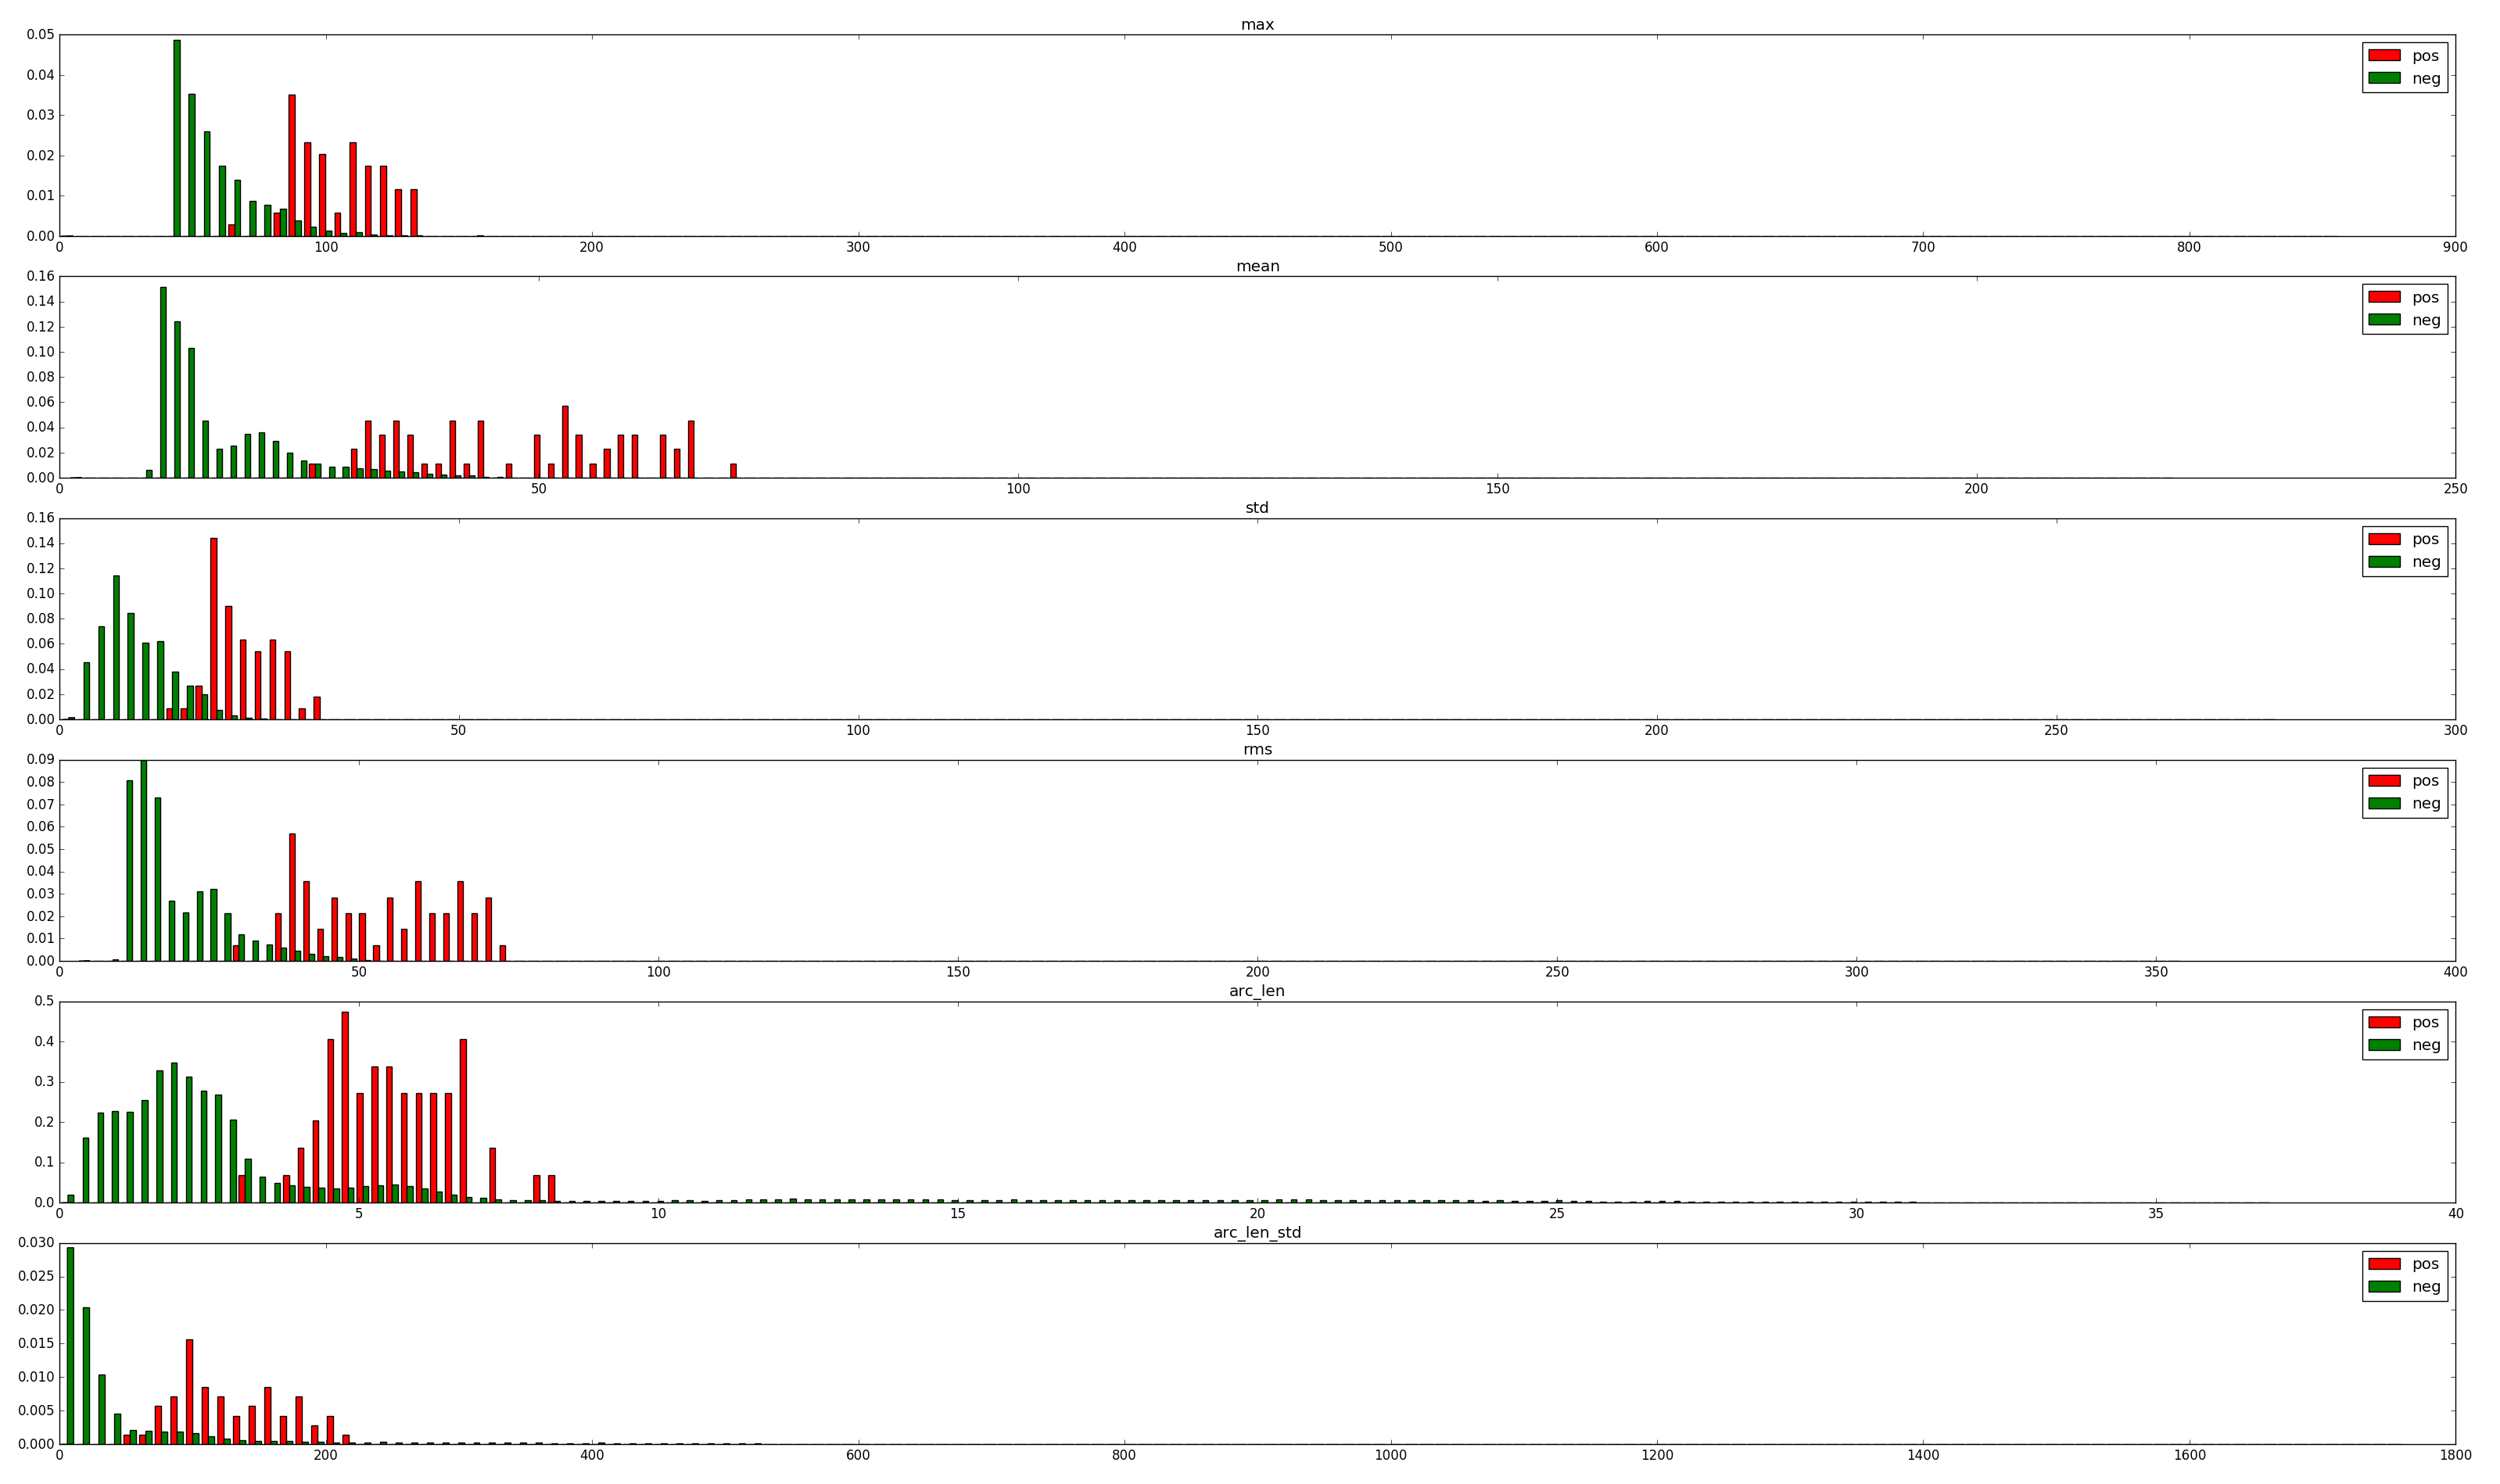
\includegraphics[width=\textwidth]{hist_features_after_win_size_1_2.png}
% \end{center}
% \caption{Histogram of feature values in the 2-second window after the~$40 m/s^2$ spike.}
% \label{fig:afterhist}
% \end{figure*}

To compare the performance of random forests and logistic regression, we fine tuned the class weights for the logistic regression classifier to lower its true positive rate until it is approximately the same as the random forests classifier, then we compared the number of false positive instances of the two classifiers.
We find that logistic regression has 14 false positive instances at a 67\% true positive rate (25 true positive instances),
while random forests has 15 false positive instances at a 62\% true positive rate (23 true positive instances).
Thus the performance of the two classifiers seems comparable in this regime.
The advantage of logistic regression is that we found adjusting class weights was more effective at controlling the false-positive/false-negative tradeoff for the logistic regression classifier.
The Receiver Operating Characteristic (ROC) curves for the logistic regression and random forests classifiers are shown in Figure~\ref{fig:roc}.

\begin{figure}[t]
\begin{center}
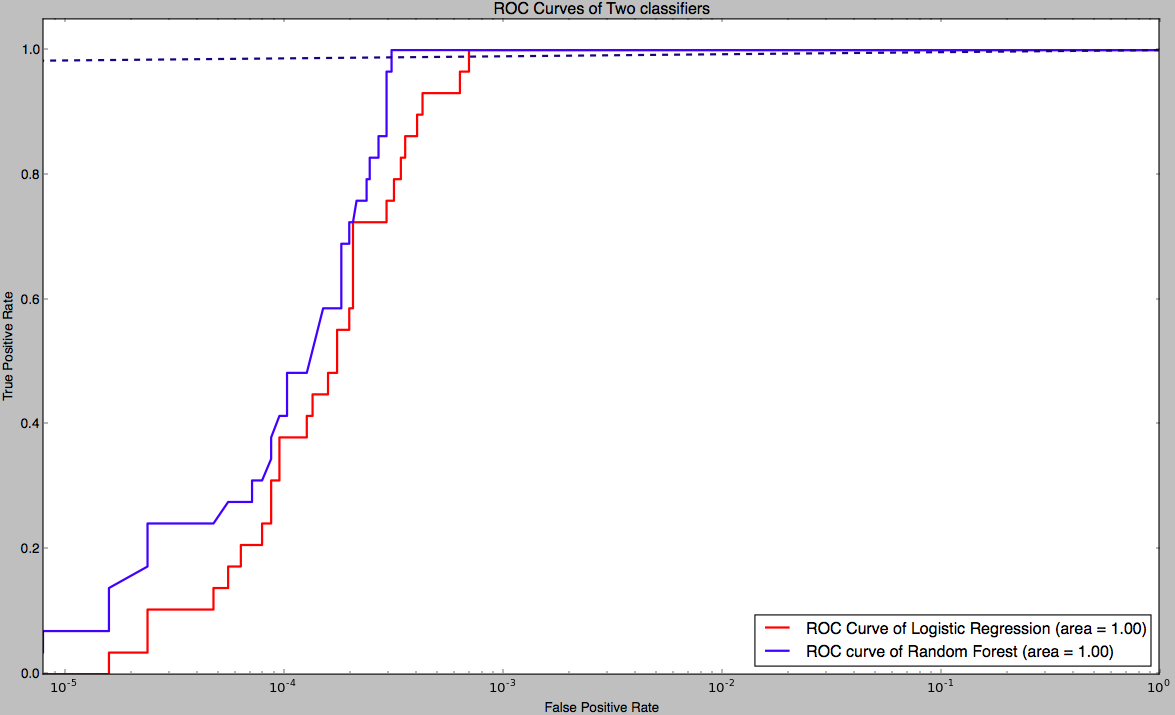
\includegraphics[width=1.0\columnwidth]{roc_curves_log_line.png}
\end{center}
\caption{ROC curves of logistic regression and random forests. The x-axis is in logarithmic scale.}
\label{fig:roc}
\end{figure}



% \section{Related Work}

Many researchers have studied using smartphone sensors for continuous user authentication.
The benefit of continuous user authentication is that it happens unobtrusively, without requiring any action from users.
Continuous authentication could serve as a mitigation for theft: if the phone can detect rapidly enough that it is no longer being used by the rightful owner, it could lock itself to prevent the thief from accessing sensitive data on the phone. 

One approach is to use smartphone accelerometer data for gait recognition.
These systems often extract some features from the sensor data and then apply machine learning.
Derawi et~al.\ achieved an equal error rate of 20\%~\cite{derawi:gait}.
``Equal error rate'' is a measure of accuracy where the system is tuned so the false accept rate and false reject rates are equal, and then that error rate is reported.
Primo et~al.\ show that accelerometer-based gait authentication is somewhat dependent on the position in which the phone is held, which is a challenge for deploying gait authentication outside of a laboratory environment~\cite{primo:context}. 
They showed how to infer the position of the phone (in the person's hand vs.\ in a pocket) with 85\% accuracy, and they showed how to use this information to increase the accuracy of user authentication to 70--80\%.
They do not report performance as equal error rate.
Juefei-Xu et~al.\ show that the pace at which people walk also affects the sensor readings, and it is possible to improve accuracy by first identifying the pace at which the user is walking, then using a model tailored towards that pace~\cite{xu:pace}.
Their system achieved an equal error rate of 4--8\% (depending on the pace); or a false reject rate of 0.5--5\% at a false accept rate of 0.1\%.
Kwapisz et~al.\ generalized gait authentication to cover not just walking but also jogging and ascending and descending stairs~\cite{kwapisz:biometrics} and
achieved false reject rates of 10--15\% at a false accept rate of about 5\%.

It is not clear whether gait recognition is sufficient on its own for deployable user authentication.
One limitation is that it can only attempt to authenticate the user while the user is walking; when the user is still, it cannot infer user identity.
Another limitation is that the error rate is still fairly high: if the classifier is run continuously, once per second, even a false reject rate as low as 0.5\% will cause hundreds or thousands of false rejections per week.
Thus, gait recognition might need to be combined with other methods to yield a deployable defense against theft.

Our work builds on the methods previous researchers have used to process sensor data and extract features.
The accelerometer sensor provides raw data in the form of $X,Y,Z$ accelerations; it is useful to also compute the magnitude $M=\sqrt{X^2+Y^2+Z^2}$ of the acceleration, as that is independent of the direction of the acceleration.
Prior papers have used several methods for cleaning the raw accelerometer data, including interpolation and re-sampling to deal with irregularly sampled data and a weighted moving average filter to mitigate sensor noise.
These schemes typically divide the resulting time series into windows, each window containing about a second of sensor data.
For instance, Primo et~al.\ used overlapping windows, with each window containing 100 samples and having an overlap of 50 samples with the next window; Derawi et~al.\ and Juefei-Xu et~al.\ used non-overlapping windows, which were about 1 second in width.
Derawi et~al.\ and Juefei-Xu et~al.\ used the sensor readings as the features, while Primo et~al.\ and Kwapisz et~al.\ computed hand-crafted features from the readings, where each feature records a summary statistic on the sensor readings in the window (e.g., mean, minimum, maximum, standard deviation, number of zero crossings, etc.).

Feng et~al.\ investigated using the unique way the user picks up their phone as a biometric for user authentication~\cite{feng:pickup}. 
They achieved an equal error rate of 6--7\%.
They used the smartphone accelerometer, gyroscope, and magnetometer; in our work, we avoid the gyroscope sensor, as its power consumption is significantly higher than the accelerometer, and therefore is currently not a practical solution for continuous authentication.

Mare et~al.\ developed a continuous authentication system where the user wears a smartwatch or bracelet, which is used to authenticate the user to their computer~\cite{mare:zebra}. 
Their continuous authentication scheme works well and could plausibly be used to authenticate to a smartphone, but it requires users to wear a bracelet; in contrast, we seek solutions that do not require the user to carry or wear any additional devices.

The most closely related work is by Chang et~al.\, who used the way
that each person takes their phone out of their bag or pocket as a 
form of biometric authentication~\cite{cheng:theft}.
They use accelerometer and gyroscope data to detect when the user picks
up their phone, and then they apply dynamic time warping and boosting to
determine whether the pickup motion matches known templates from the
owner of the phone.
Their system achieves a 10\% false positive rate and a 5.5\% false negative rate, which are relatively high,
considering that users may pick up their phones dozens of times each day.

The prior work focuses on authenticating the user.
In contrast, we take a different approach: we attempt to detect the
specific motion pattern that occurs during a grab-and-run or pickpocket theft.
The benefit of biometric authentication is that it provides a comprehensive
way to detect theft, regardless of the way the phone was stolen; however,
as summarized above, the false positive rates of existing schemes
are fairly high.
Our scheme is limited to detecting a particular type of theft, but achieves
far lower false positive rates.
Our classifier is also user-independent and does not require obtaining
training data from each user; we use the same classifier for all users.




\section{Methodology}

In this section, we describe the data collection software, which we used to gather positive and negative data for our training and test sets as well as the feature extraction scheme, and other classifier design decisions.

\subsection{Data Collection}

\subsubsection{Software}
We used an Android application to record data from the smartphone's 3-axis accelerometer, which then encrypted it and stored it in the cloud.
We acquired sensor data at the highest sampling rate supported by the phone using SENSOR\_DELAY\_\\FASTEST~\cite{android:doc}. 
On most devices, including the one we used for the simulated theft experiment, the sampling rate is 100 Hz. 

\subsubsection{Simulated Theft Experiment}
Because data from real thefts is hard to obtain, we simulated three types of common smartphone theft scenarios, based on campus police alerts that we receive, with one researcher acting as a smartphone user and another one playing the role of a thief. 
The three theft scenarios are as follows:
\begin{enumerate}
\item The user stands still and holds the phone with one hand as she is using the device, for instance reading a text; the thief approaches from behind, grabs the phone with both hands and runs away in the forward direction. 
\item The user holds the phone in front of her with one hand while walking at a constant speed; the thief approaches from behind, grabs the phone with both hands and runs away in the forward direction. 
\item The third scenario simulates pick-pocket thefts. The user places the phone in the back pocket of their pants and stands still; the thief approaches from behind, steals the phone from user's pocket and runs away in the forward direction.
\end{enumerate}
We collect 40 instances of each scenario, for a total of 120 trials. 
Data collection was split across four sessions, each consisting of 10 trials per scenario, with different researchers acting as the victim and thief in these two sessions. 
We ran the experiment on flat ground in an open space, so the experiment was not interrupted. 
We also made sure that the thief ran at least 40 feet after gaining possession of the victim's phone.
We used a Nexus 5X smartphone (InvenSense MPU6515 embedded accelerometer) with Android version 7.1.1 for data collection in our simulated theft experiment.
Figure~\ref{fig:simtheft} plots one example of accelerometer readings from a single simulated theft.


\begin{figure}[t]
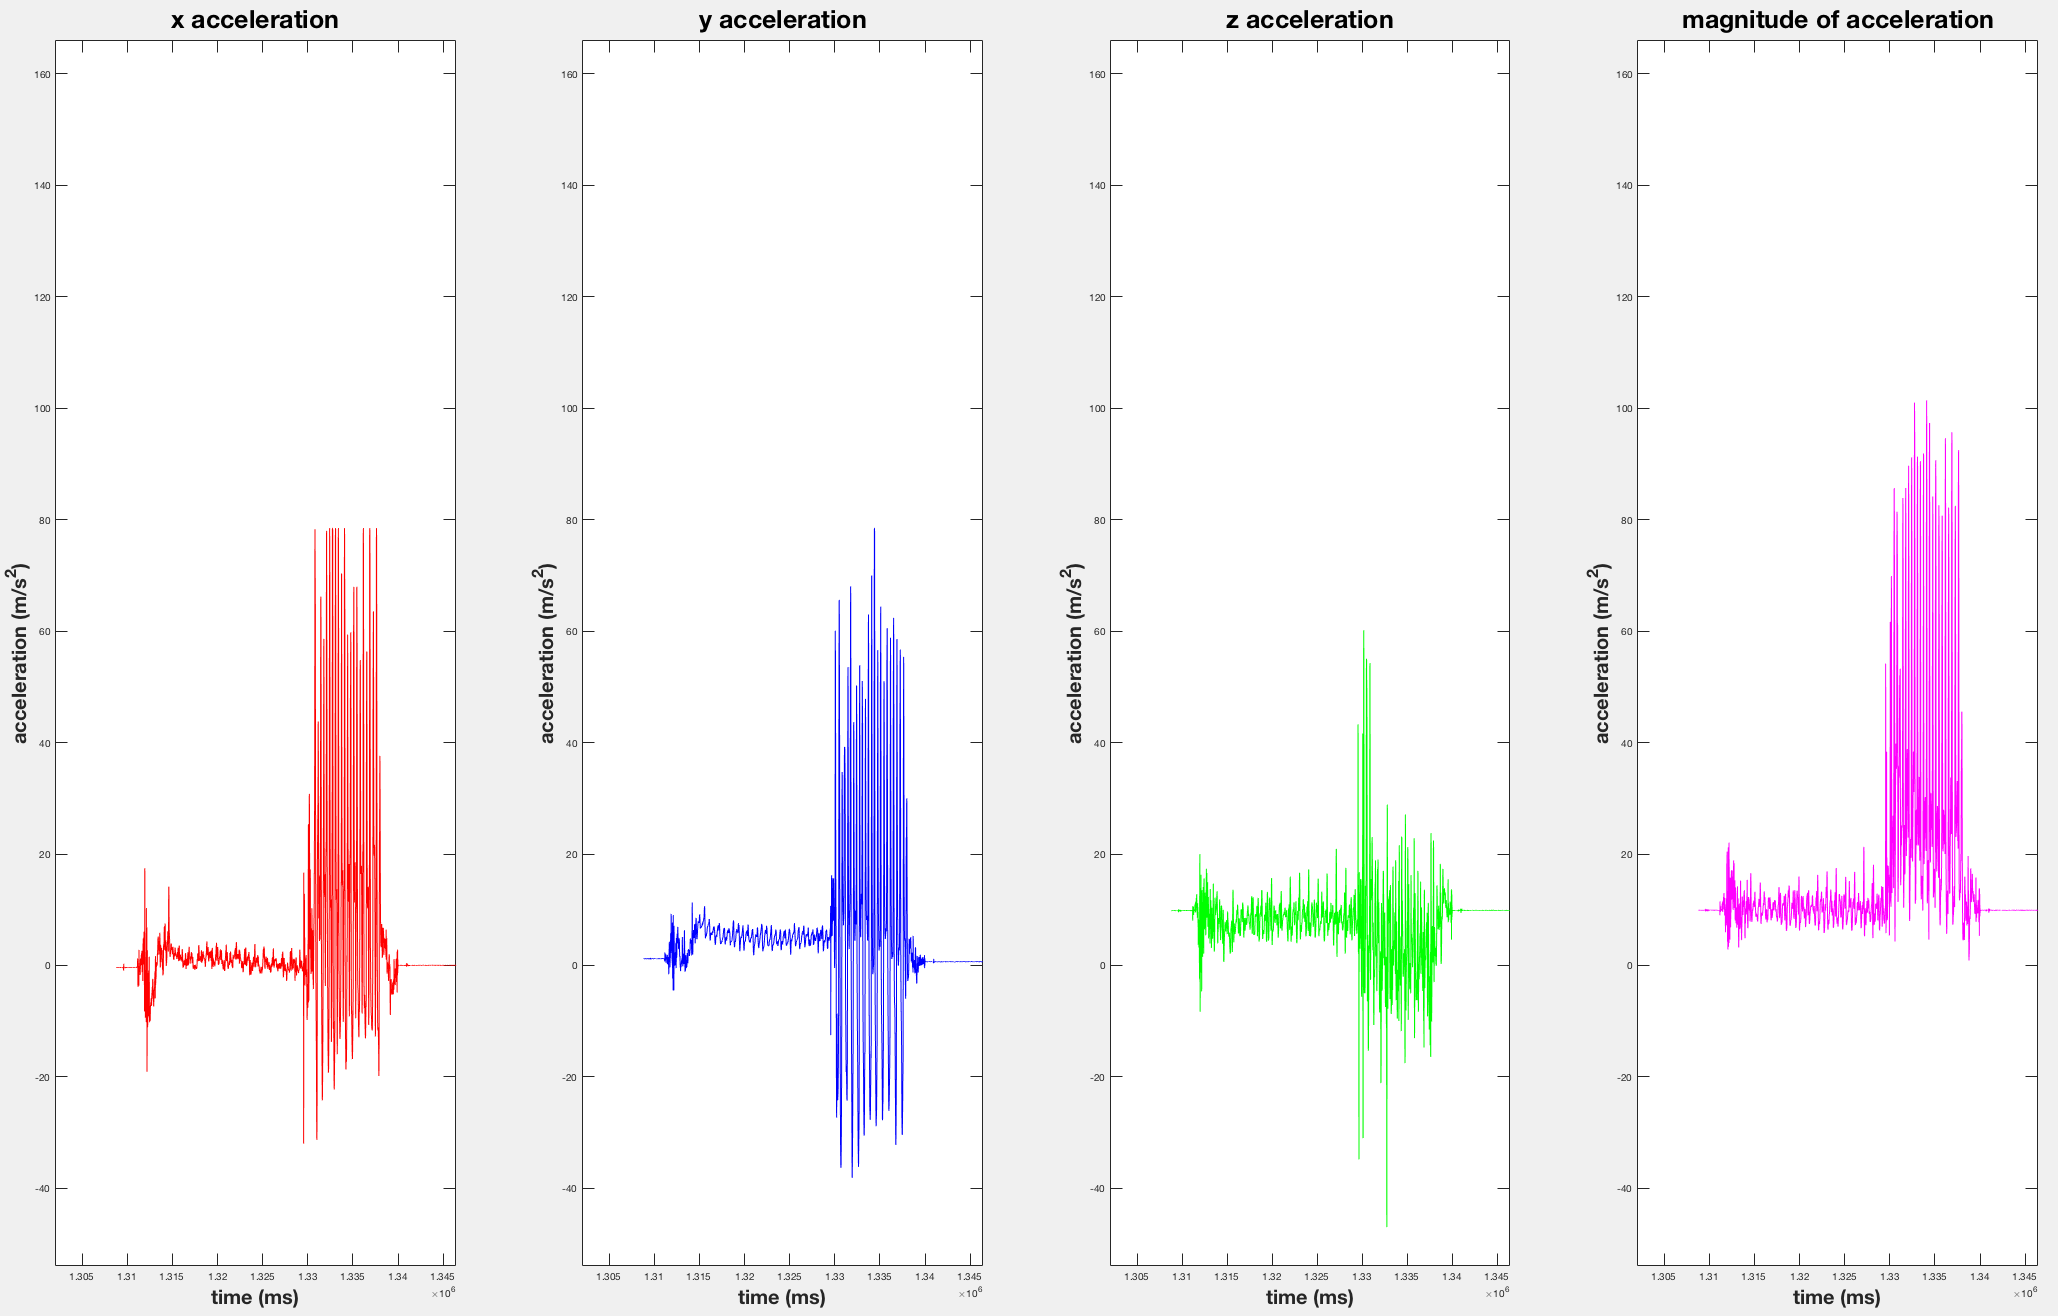
\includegraphics[width=1.0\columnwidth]{pos_acc_separated.png}
\caption{The X, Y, Z and magnitude of acceleration, respectively, from one simulated theft instance.}
\label{fig:simtheft}
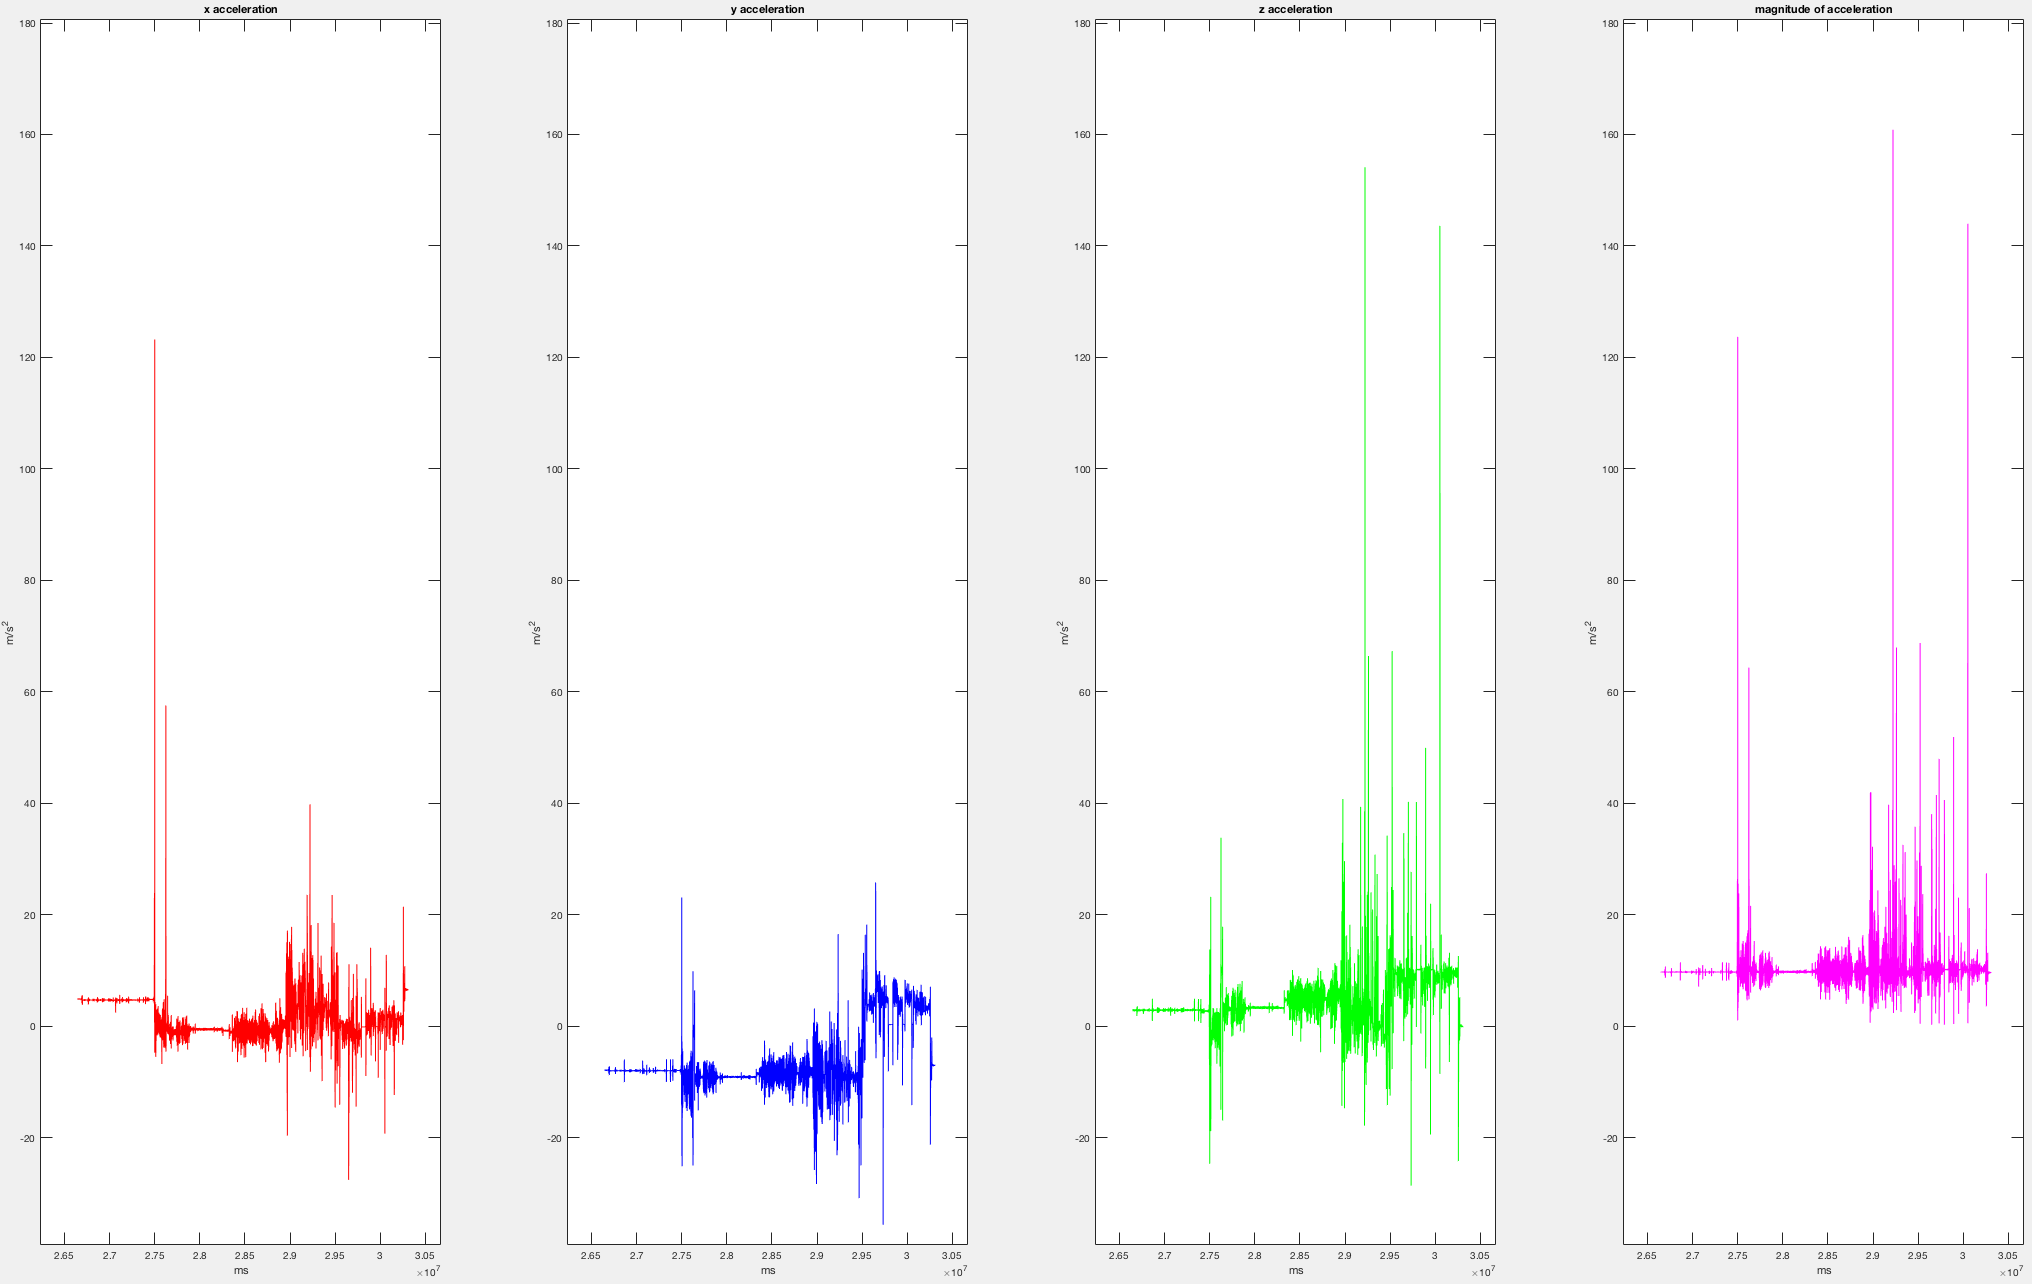
\includegraphics[width=1.0\columnwidth]{neg_acc_separated.png}
\caption{The X, Y, Z and magnitude of acceleration, respectively, during normal usage at an arbitrary time period.}
\end{figure}




\subsubsection{Field Study}
We performed a field study to gather data from ordinary smartphone users while they perform everyday activities, including walking, running, driving, possibly excercising, and anything else that occurred during their lives over the field study period.
% We obtained approval from the University of California, Berkeley IRB (Institutional Review Board) for this study. 
We obtained approval from our university IRB for this study. 
The study was conducted in a metropolitan area from September to December 2016.
% The study was conducted in the Bay Area of the United States from September to December 2016.
None of the participants experienced a phone theft during the study interval,
so we were able to use the accelerometer data collected from the user study as negative samples for our machine learning algorithms (i.e., instances of non-theft activity).

We posted a recruitment advertisement on Craigslist in September 2016. 
% We posted a recruitment advertisement on the Craigslist under the SF Bay Area `jobs et cetera' category in September 2016. 
We only recruited participants who used an Android smartphone with version 5.0 and above. 
After obtaining their consent, we installed our data collection application on their phones and collected data for a three-week period.
The application ran in the background and collected accelerometer sensor readings continuously, 24 hours a day.
We contacted participants weekly to make sure their phones were functioning correctly and troubleshoot any data collection issues.
Each participant was paid \$150 for their participation.

The study was divided across 3 rounds; each round lasted 3 consecutive weeks. 
A total of 55 participants were recruited, and
53 out of the 55 subjects completed the study. 
In the first round, 2 of the 18 participants did not complete the study.
Detailed demographic information about the participants of this user study is listed in Table~\ref{tbl:demographics}.
In aggregate, they used 21 different smartphone models from 6 different manufacturers and 8 different Adroid versions. This ensures the dataset containing diverse devices, and the classifiers are not specific to a particular type of smartphone or Adroid version.
We also asked participants how they typically carried their phone, when it was not in their hands; 33 reported keeping it in their pockets, 9 in their purses, 12 in multiple locations (e.g., pocket or purse, pocket or backpack), and 1 did not respond.
During the study, the subjects carried their phones while performing daily activities, for example walking, driving, running and possibly excercising. Data from a wide variety of real-world activities ensures the generability of the classifiers trained on it. 

\begin{table}[H]
\centering
\begin{tabular}{rrrrrr}
\hline
      & Male & Female & Age 20--29 & 30--39 & 40+ \\ \hline
R1    & 5    & 11     & 8         & 6     & 2   \\
R2    & 10   & 8      & 7         & 7     & 4   \\
R3    & 11   & 8      & 9         & 4     & 6   \\
Total & 26   & 27     & 24        & 17    & 12  \\ \hline
\end{tabular}
\caption{Participants' demographic information.}
\label{tbl:demographics}
\end{table}




\subsection{Feature Extraction}
\label{s:features}

Our theft scenarios all involved a sudden movement of the phone, which causes a large acceleration.
Therefore, as a first filtering step, we filtered the data to focus on times near when a large motion occurs.
In particular, our classifier is activated when the magnitude of acceleration $M$ exceeds~$40 m/s^2$.
We extract a one-second window before the activation time and a $n$-second window after the activation time, compute features on each of these windows, and use them for classification.
We vary $n$ from 1 to 7 to obtain the best classification accuracy.
We chose a threshold of~$40 m/s^2$ as all of our simulated thefts experienced accelerations exceeding that threshold when the phone was initially grabbed by the thief.

We first identified 16 candidate features, 8 features for each of the two windows.
In particular, we computed the minimum, maximum, mean, standard deviation, root mean square, arc length, product of arc length and standard deviation, and mean absolute value, each computed on the magnitude values ($M$) within the window.
We chose to only compute these features on the magnitude of the acceleration, and not the $X$, $Y$, and $Z$ components, because the magnitude is non-directional and thus more robust to changes in the orientation of the phone. 
We then visualized the distribution of these features for the two classes and applied feature selection techniques to choose a subset of features that yield good performance.
We removed the minimum and mean absolute value from the feature list because removing them did not affect the performance of the classifiers. 
As a result, we extract a 12-dimensional feature vector, 6 features from the before-window and 6 from the after-window, every time the detector is triggered.

Let $M_1,\dots,M_k$ denote the time series of acceleration magnitudes within the window.
The features are computed as follows:
\begin{itemize}
\item \emph{Maximum}: the maximum value of the magnitude within the window, i.e., $\max(M_1,\dots,M_k)$.
\item \emph{Mean}: the average value of magnitude in a window, i.e., $(M_1+\dots + M_k)/k$.
\item \emph{Standard deviation}: the standard deviation of magnitude values in a window.
\item \emph{Root mean square}: the RMS of magnitude values in a window, i.e., $(M_1^2 + \dots + M_k^2)^{1/2}/k^{1/2}$.
\item \emph{Arc length}: the average of the absolute differences between all adjacent magnitude values in a window, i.e., $(|M_2-M_1| + |M_3-M_2| + \dots + |M_k-M_{k-1}|)/(k-1)$.
Intuitively, this captures the average of the first derivative of the acceleration.
\item \emph{Product of arc length and standard deviation}: the product of the two feature values.
\end{itemize}

Because the accelerometer sensor reports readings in the same units on all Android phones, and because our features are relatively simple, we believe these features capture fundamental, device-independent characteristics of the motion rather than anything specific to the particular device used for data capture (e.g., in contrast to the hardware-based differences documented by Dey et al.~\cite{Dey2014}).

We obtained 60 positive instances from the 60 simulated thefts.
After applying the~$40 m/s^2$ threshold, we obtained approximately approximately 248,000 negative samples from the data collected in the field study. 
We then applied boolean classification techniques to this data set.


% \begin{figure}[t]
% 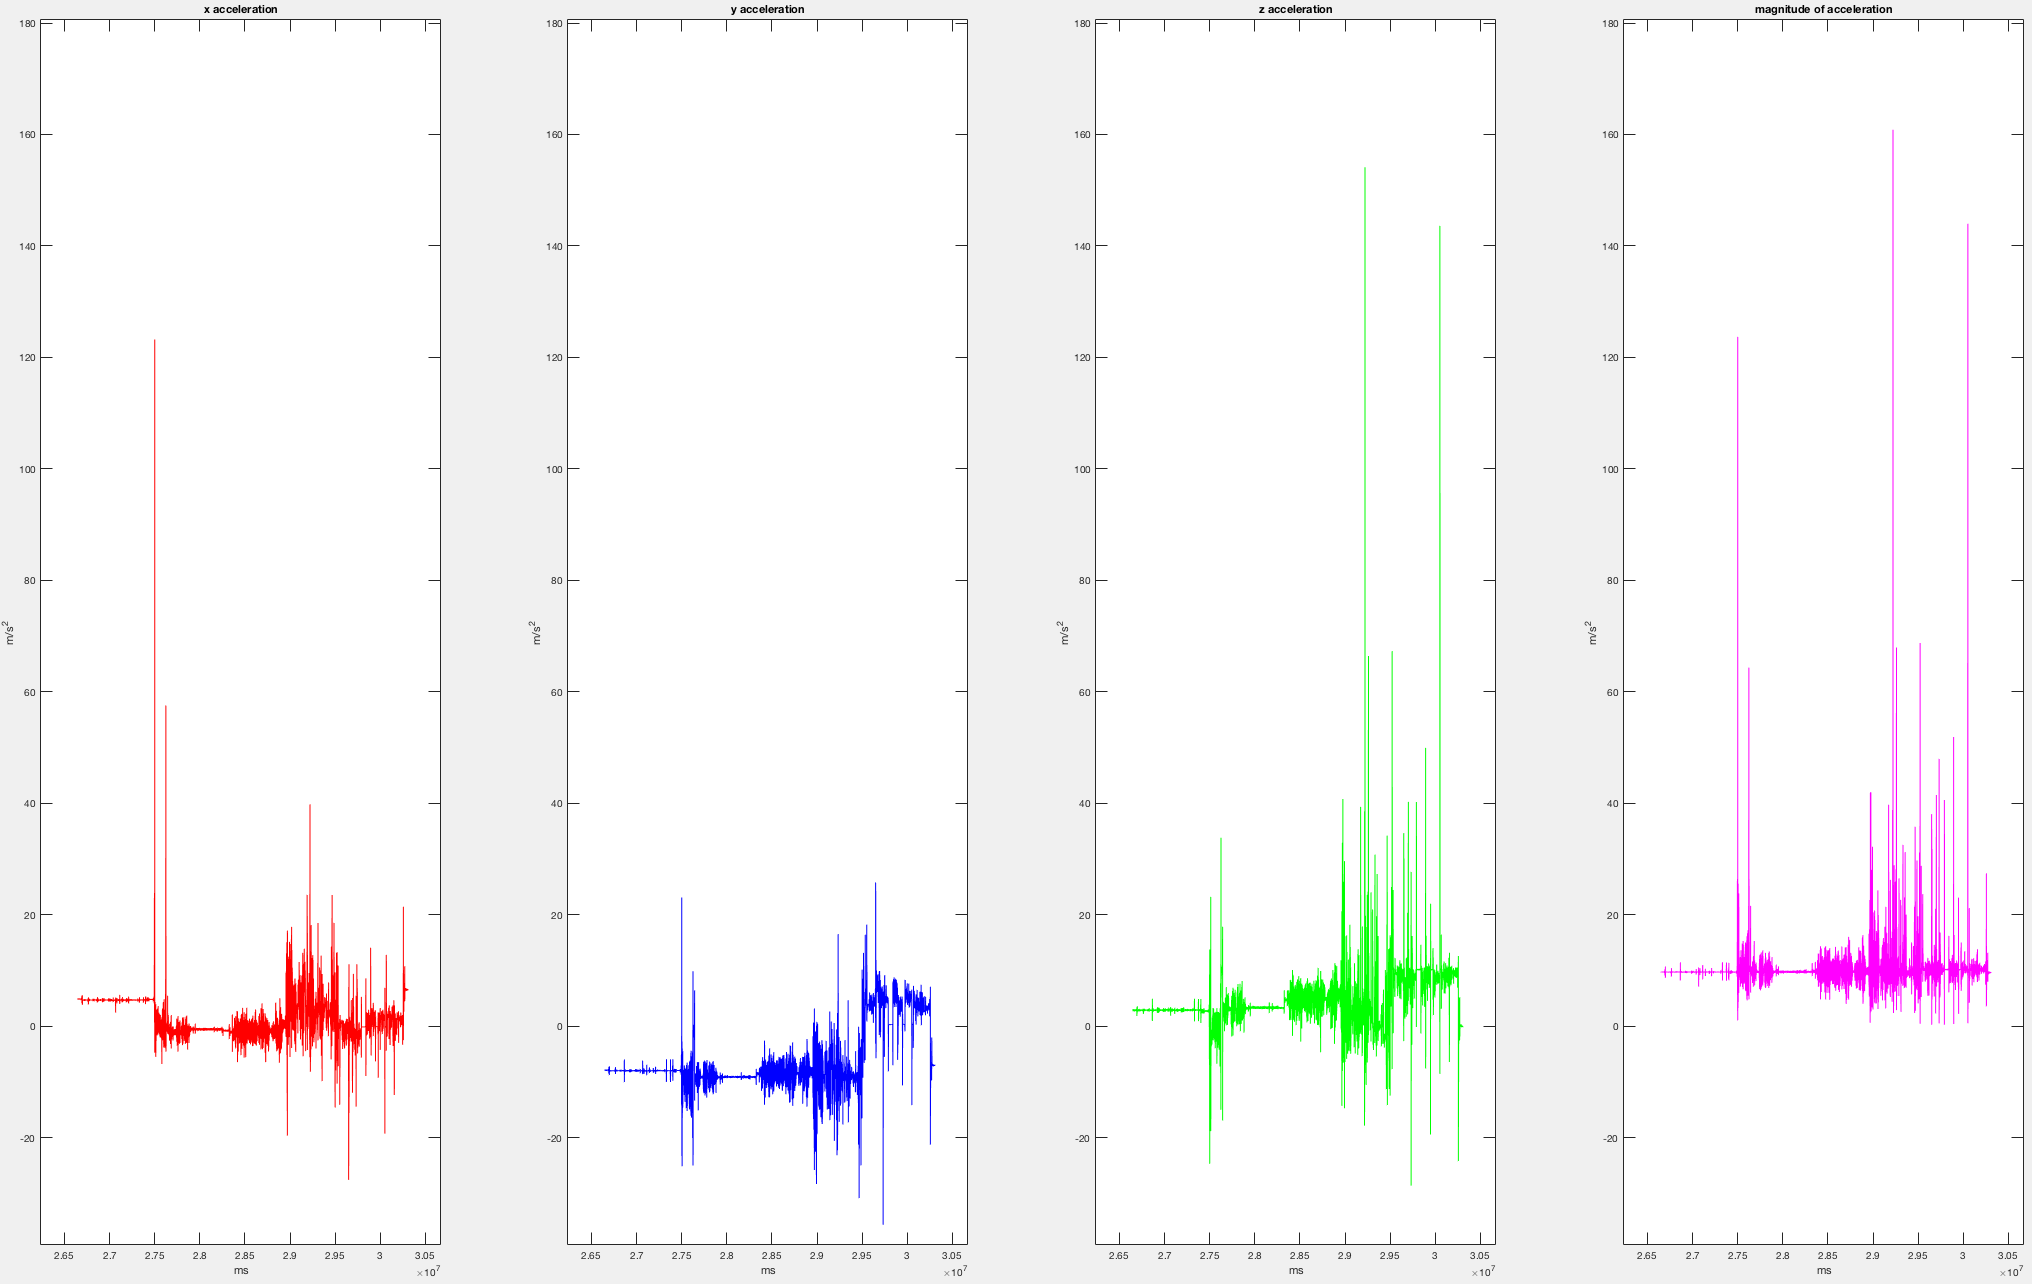
\includegraphics[width=1.0\columnwidth]{neg_acc_separated.png}
% \caption{The X, Y, Z and magnitude of acceleration, respectively, during normal usage at an arbitrary time period.}
% \end{figure}



\subsection{Machine Learning Algorithms}
We evaluate three standard machine learning algorithms: linear SVM, logistic regression and random forests.
Because we have many more negative samples than positive ones, we tried different settings for class weights to weight positive instances more highly than negative ones.
We also evaluated different window sizes for the after-window.
We found that a 2-second after-window yielded better accuracy than a 1-second after-window since 2-second windows encapsulate more complete acceleration information about the motions, and larger window sizes did not offer much improvement.
Therefore, all of our experiments use a 1-second before-window and a 2-second after-window.
We partitioned the entire dataset, which consists of 120 positive samples and approximately 248,000 negative samples, into training and test sets with 7:3 ratio.
Then we trained the classifiers on the training set and reported the predition results of the test set.



\section{Results}
Among the three classifiers, logistic regression performs the best.
Confusion matrices for logistic regression, random forests, and a linear SVM
are shown in Table~\ref{fig:cmat}.
The logistic regression classifier has a false positive rate of 0.09\%. Given that the field study involved 53*3=159 person-week of data, and the logistis regression would report 248,000*0.09\%=223 false positives, the total number of samples extracted from the field study data times the false positive rate. This means that on average users receive 223/159$\approx$1.4 false alarm every week, and a true positive rate of 100\%.
The random forests classifier has an even lower false positive rate (approximately one false alarm per month),
but it only detects 60\% of the thefts.

Only a small fraction of predicted positives will actually be theft, but we expect this will be acceptable due to the relatively low cost of false positives: it means users will have to unlock their phones one extra time per week, which seems likely to be tolerable. We report the false positive rate rather than precision, because the false positive rate is easily interpretable and not sensitive to the rate at which theft occurs. The precision is sensitive to the number of simulated thefts included in the dataset, which might not match the number of actual thefts that are likely to occur over a given period of time.


\begin{table}[t]
\centering
\begin{tabular}{@{}lll@{}}
\toprule
              & Predicted Negative & Predicted Positive \\ \midrule
True Negative & 74446              & 72                 \\
True Positive & 0                  & 37                 \\ \bottomrule
\end{tabular}

\begin{tabular}{@{}lll@{}}
\toprule
              & Predicted Negative & Predicted Positive \\ \midrule
True Negative & 74503              & 15                 \\
True Positive & 14                 & 23                 \\ \bottomrule
\end{tabular}

\begin{tabular}{@{}lll@{}}
\toprule
              & Predicted Negative & Predicted Positive \\ \midrule
True Negative & 74501              & 17               \\
True Positive & 17                 & 20                 \\ \bottomrule
\end{tabular}
\caption{Confusion matrices for a logistic regression classifier (at top; with class weights 1:200), random forests classifier (middle; class weights 1:5000), and a linear SVM classifier (bottom; class weights 1:1000).}
\label{fig:cmat}
\end{table}

% \begin{table}[t]
% \centering
% \begin{tabular}{@{}lll@{}}
% \toprule
%               & Predicted Negative & Predicted Positive \\ \midrule
% True Negative & 248223             & 170                \\
% True Positive & 0                  & 60                 \\ \bottomrule
% \end{tabular}
% \caption{Confusion matrix for a logistic regression classifier trained
% with class weights set to 1:200.}
% \label{fig:logistic}
% \end{table}

% \begin{table}[t]
% \centering
% \begin{tabular}{@{}lll@{}}
% \toprule
%               & Predicted Negative & Predicted Positive \\ \midrule
% True Negative & 248360             & 33                 \\
% True Positive & 32                 & 28                 \\ \bottomrule
% \end{tabular}
% \caption{Confusion matrix for a random forests classifier trained with
% class weights set to 1:5000.}
% \label{fig:rf}

% \end{table}

% \begin{table}[t]
% \centering
% \begin{tabular}{@{}lll@{}}
% \toprule
%               & Predicted Negative & Predicted Positive \\ \midrule
% True Negative & 246522             & 1871               \\
% True Positive & 42                 & 18                 \\ \bottomrule
% \end{tabular}
% \caption{Confusion matrix for a linear SVM classifier trained with
% class weights set to 1:1000.}
% \label{fig:svm}
% \end{table}


To get a better understanding of why our classifier is successful,
we computed feature rankings to find the most predictive features.
For logistic regression, we used standardized coefficients as the feature importance score:
the score for feature $i$ is $|\alpha_i| \cdot \sigma_i$, where $\alpha_i$ is the coefficient for feature $i$ in the logistic regression model and $\sigma_i$ is the standard deviation of feature $i$ in the training set.
In addition, we computed the 95\% confidence intervals for all standardized coefficents using 50 epoches of the entire data set.
The feature importance scores and their 95\% confidence intervals for the logistic regression classifier are listed in Table~\ref{tbl:importance-lr}.
The most discriminative features are
the maximum of the before-window,
the product of arc length and standard deviation of the after-window,
and the arc length of the before-window.
Plotting a histogram of feature values (see Figures~\ref{fig:beforehist} and \ref{fig:afterhist}), we can see that those features do appear to provide good discrimination.


\begin{table}[t]
\centering
\begin{tabular}{@{}ll@{}}
\toprule
Feature                & Feature Importance \\ \midrule
Root mean square (b)   &   143.8786849  ($\pm$ 0.08714717)       \\
Mean (b)               &   129.8910092 ($\pm$ 0.08033373)       \\ 
Root mean square (a)   &  \ 93.8382532  ($\pm$ 0.04439512)       \\
Mean (a)               &  \ 88.1273891  ($\pm$ 0.03972303)       \\
Standard deviation (a) &  \ 66.7204655  ($\pm$ 0.02228971)       \\
Standard deviation (b) &  \ 47.7685313  ($\pm$ 0.03349549)       \\
Arc length (a)         &  \ 27.3736785  ($\pm$ 0.01463394)       \\
Maximum (b)            & \ \ 2.73231469 ($\pm$ 0.00041407)       \\
Arc length * SD (a)    & \ \ 2.69875036 ($\pm$ 0.00097762)       \\
Arc length (b)         & \ \ 1.16578948 ($\pm$ 0.00855526)       \\
Maximum (a)            & \ \ 0.05985700 ($\pm$ 0.00065551)       \\
Arc length * SD (b)    & \ \ 0.04950325 ($\pm$ 0.00090281)       \\ \bottomrule

\end{tabular}
\caption{Feature importances and their 95\% confidence intervals for logistic regression. (b) denotes the features extracted from the 1s window before the 40-spike; (a) denotes the features extracted from the 2s window after the 40-spike.}
\label{tbl:importance-lr}
\end{table}

We also rank the features for the random forests classifier using scikit-learn's feature importance score, which estimates the relative importance of the features by computing the expected fraction of the samples they contribute to. 
Thus the higher in the tree, the more important the feature is~\cite{sklearn:rfdoc}. 
% 0.04751106, 0.0080411, 0.02881483, 0.01533719, 0.02245781, 0.03309431, 0.12388036, 0.20288397, 0.16426152, 0.21908845, 0.05162059, 0.0830088.
We also computed the 95\% confidence intervals for all feature importance scores using 50 epoches of the entire data set.
The resulting feature importance scores and their 95\% confidence intervals for the random forests classifier are listed in Table~\ref{tbl:importance-rf}.

% Another way to visulize the representative features is to plot a histogram of dataset and to see which features can better seperate the positive and negative data points, as shown in Figures 1 and 2.

\begin{table}[t]
\centering
\begin{tabular}{@{}ll@{}}
\toprule
Feature                & Feature Importance \\ \midrule
Root mean square (a)   & 0.24251892 ($\pm$ 0.00734018)         \\
Mean (a)               & 0.19351276 ($\pm$ 0.00685086)         \\
Standard deviation (a) & 0.17634030 ($\pm$ 0.00601571)         \\
Maximum (a)            & 0.10975278 ($\pm$ 0.00480411)         \\
Arc length * SD (a)    & 0.07541471 ($\pm$ 0.00382659)         \\
Arc length (a)         & 0.04821400 ($\pm$ 0.00264303)         \\
Maximum (b)            & 0.04740376 ($\pm$ 0.00172894)         \\
Arc length * SD (b)    & 0.03291854 ($\pm$ 0.00128944)         \\
Standard deviation (b) & 0.02828350 ($\pm$ 0.00115971)         \\
Arc length (b)         & 0.02072662 ($\pm$ 0.00103551)         \\
Root mean square (b)   & 0.01544474 ($\pm$ 0.00078121)         \\
Mean (b)               & 0.00946937 ($\pm$ 0.00077147)          \\ \bottomrule
\end{tabular}
\caption{Feature importances and their 95\% confidence intervals for random forests. (b) denotes the features extracted from the 1s window before the 40-spike; (a) denotes the features extracted from the 2s window after the 40-spike.}
\label{tbl:importance-rf}
\end{table}


% \begin{figure*}[t]

% \begin{center}
% \begin{minipage}
% 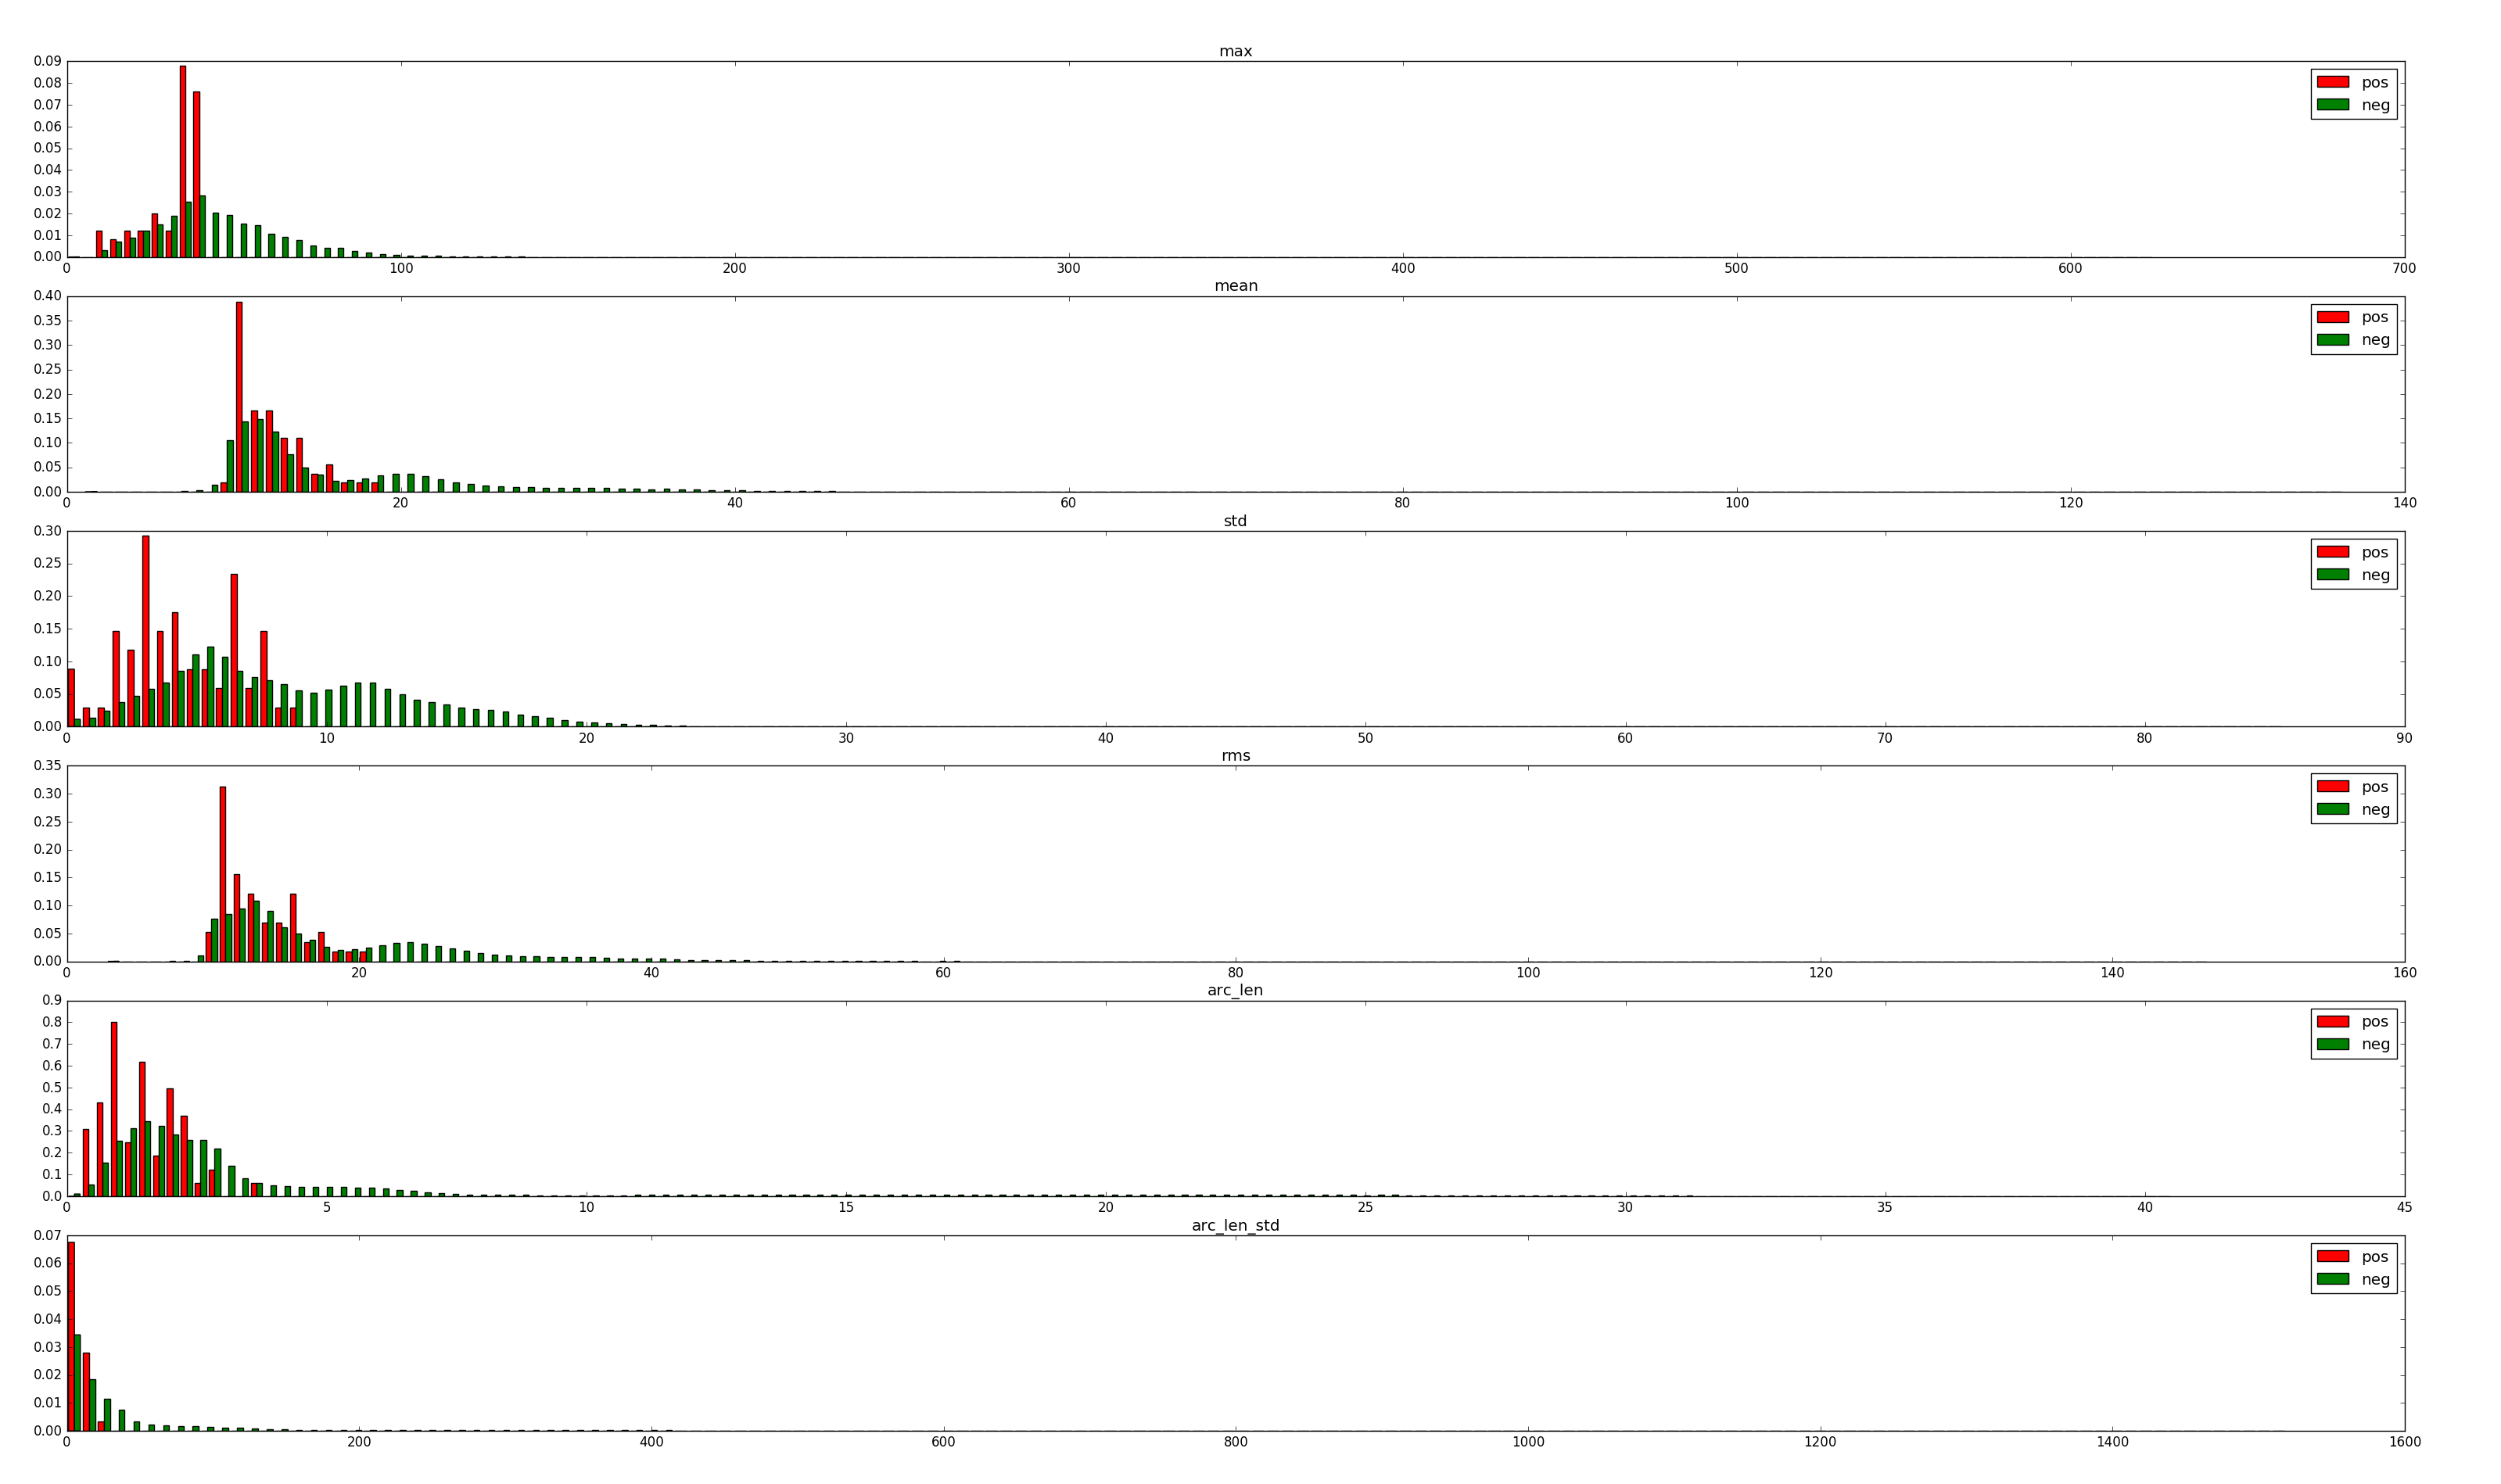
\includegraphics[width=\textwidth]{hist_features_before_win_size_1_2.png}
% \end{minipage}
% \end{center}
% \caption{Histogram for each of the 6 features for the 1-second window before the~$40 m/s^2$ spike.  The features are listed in the order presented in Section~\ref{s:features}, e.g., the top histogram is for the maximum.  Red bars indicate thefts, and green bars indicate non-theft windows.}
% \label{fig:beforehist}
% \begin{center}
% \begin{minipage}
% 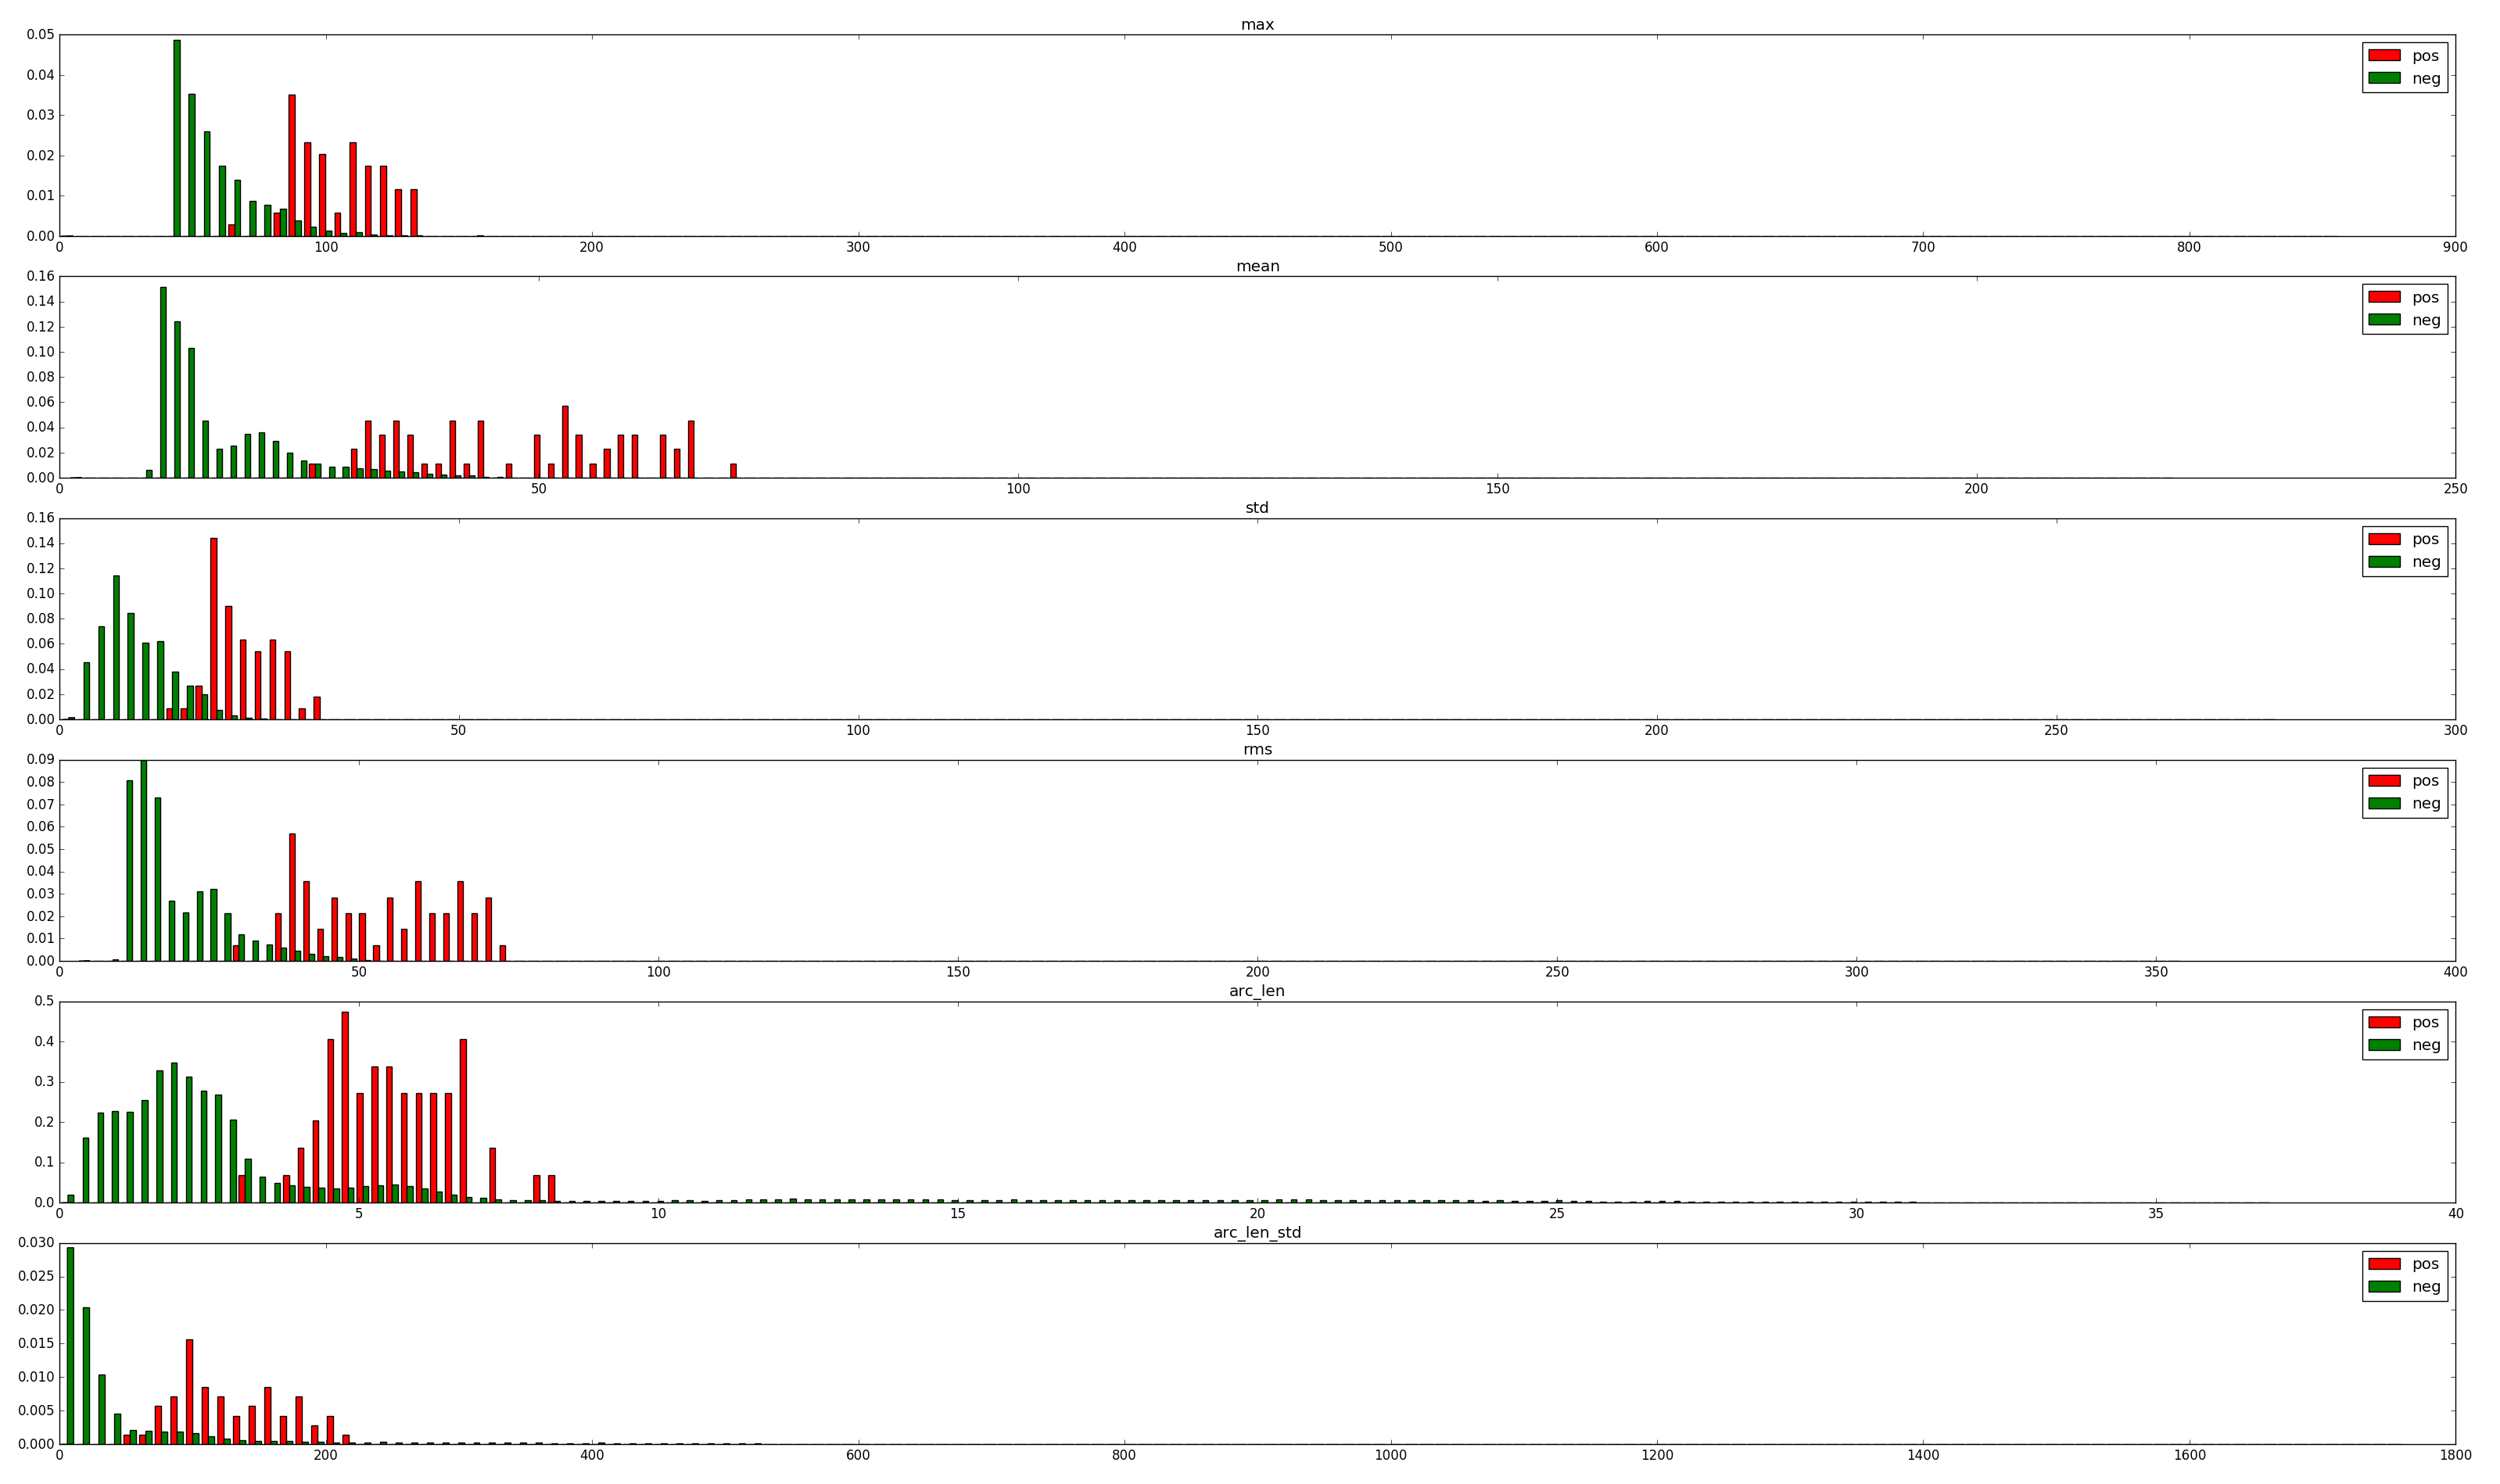
\includegraphics[width=\textwidth]{hist_features_after_win_size_1_2.png}
% \end{minipage}
% \end{center}
% \caption{Histogram of feature values in the 2-second window after the~$40 m/s^2$ spike.}
% \label{fig:afterhist}

% \end{figure*}


\begin{figure*}[t]
\centering
\begin{minipage}[t]{\columnwidth}
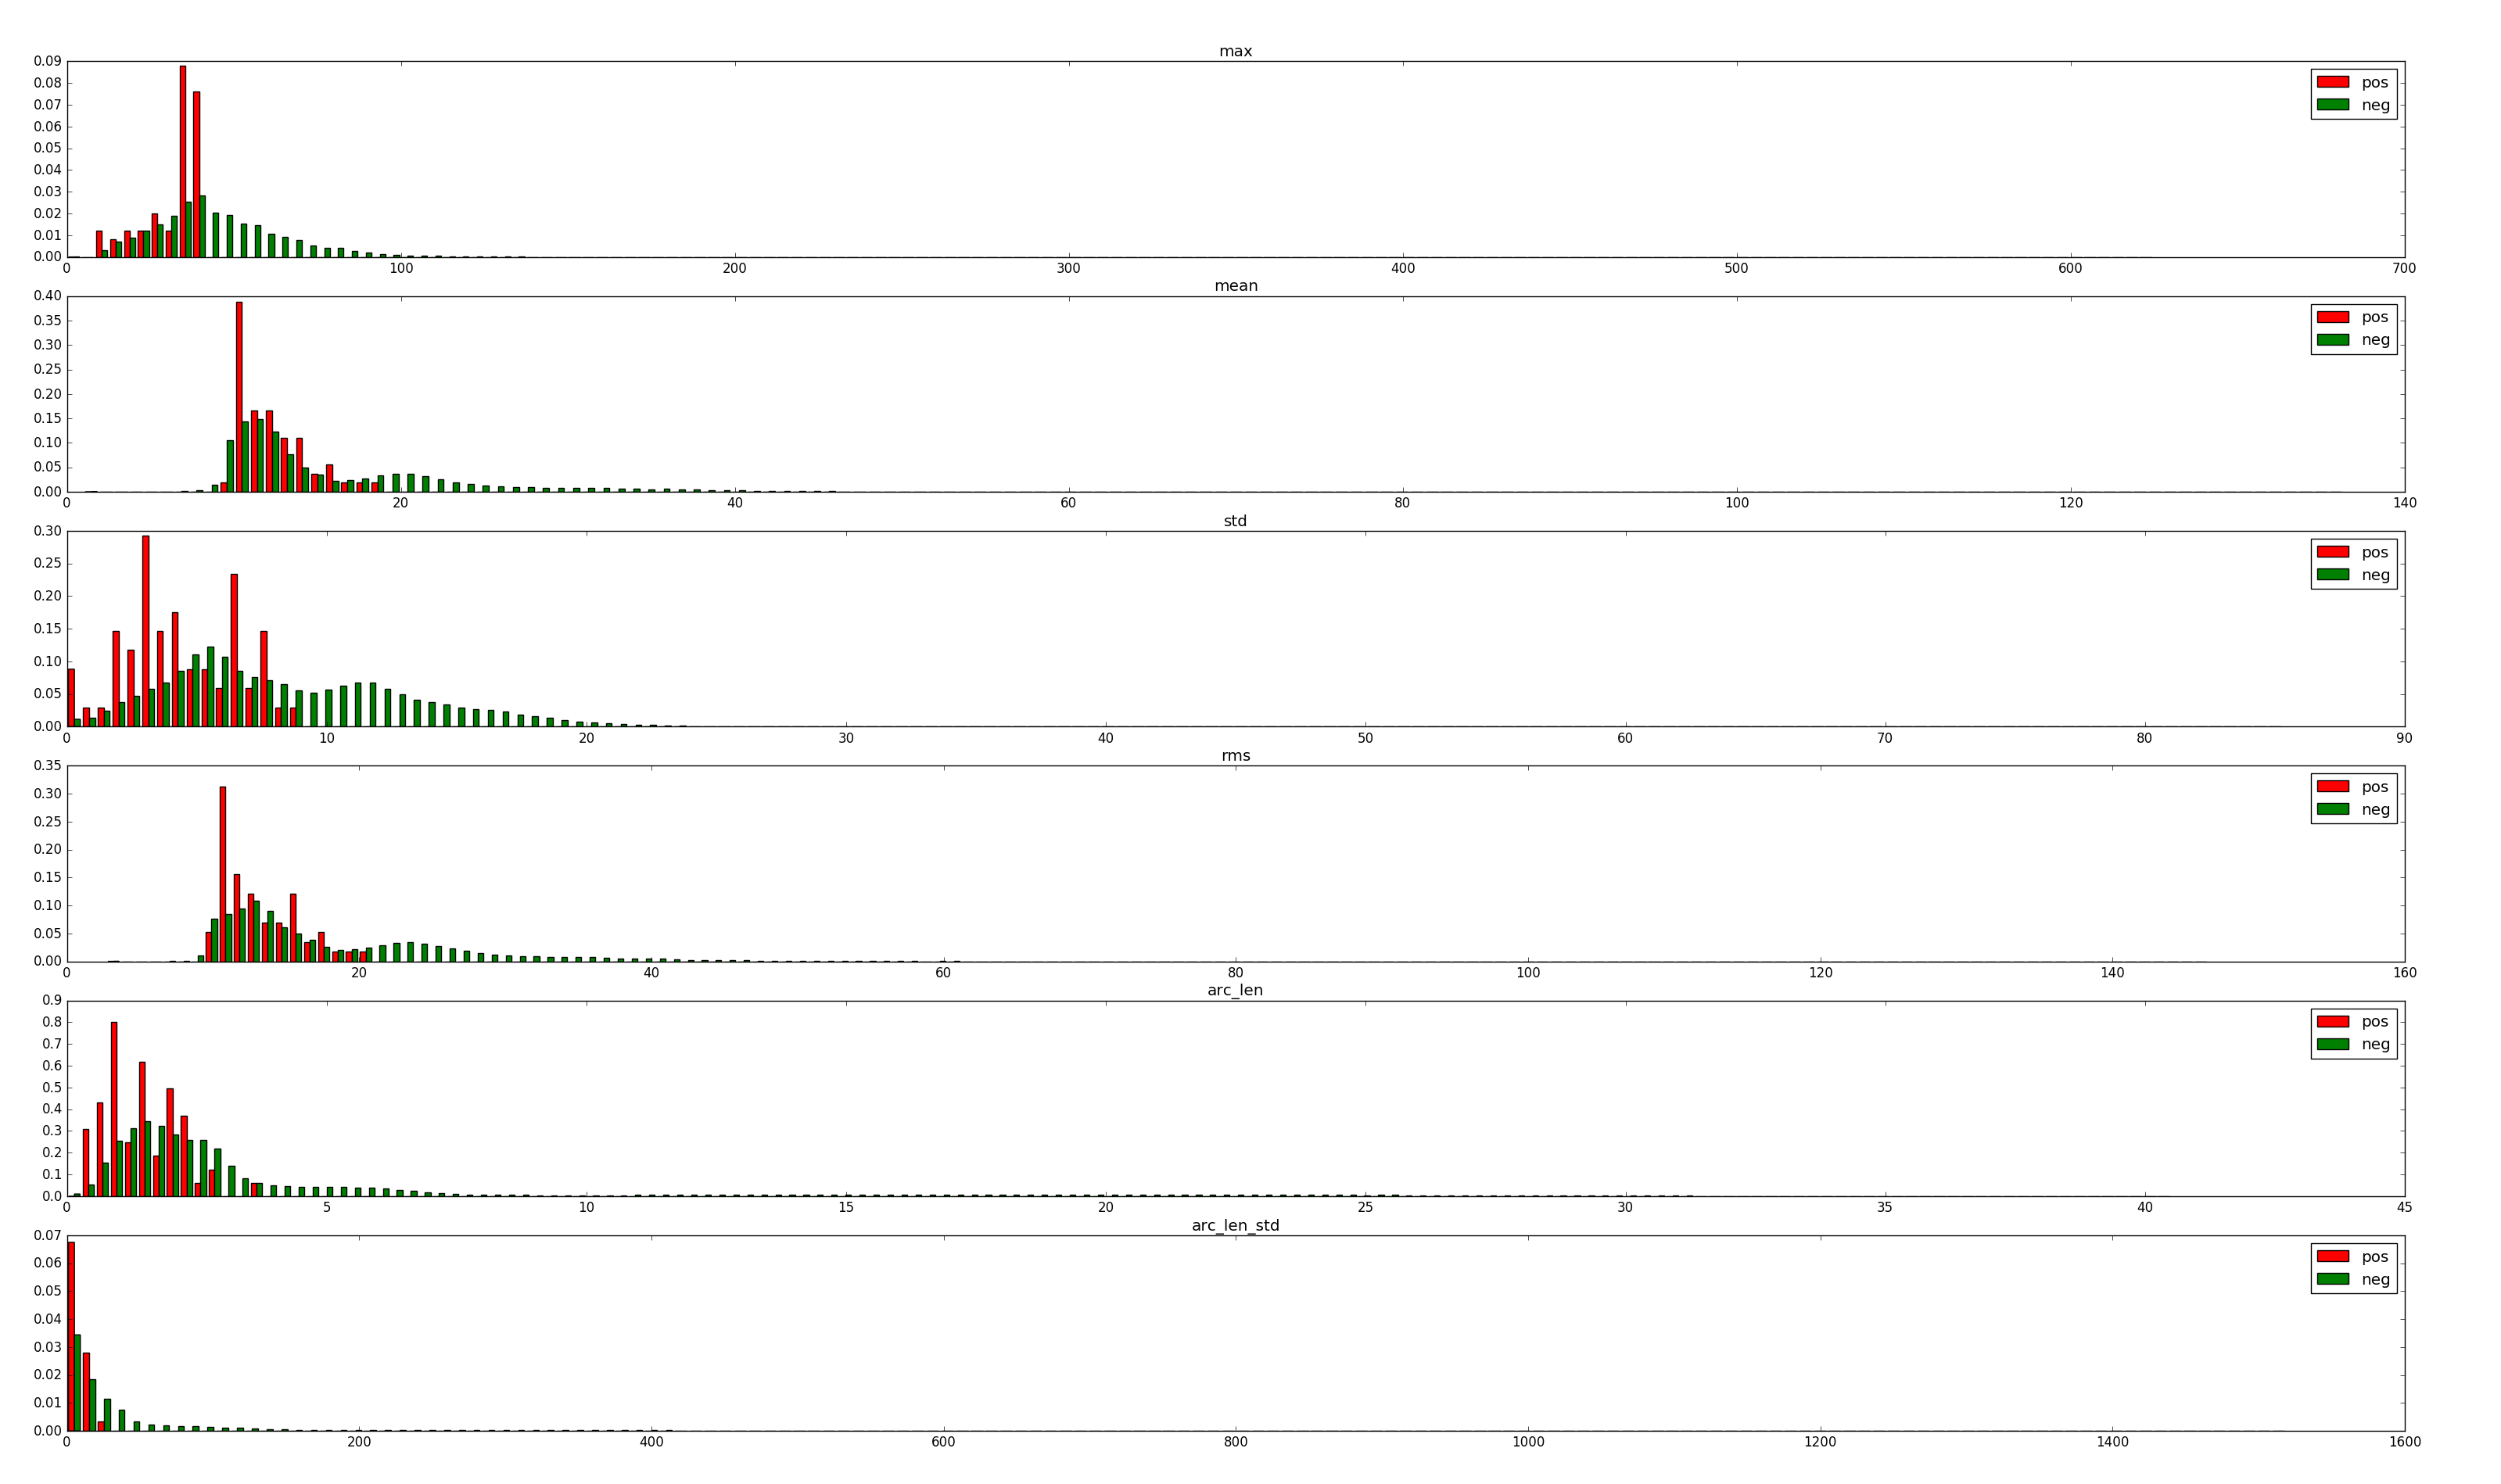
\includegraphics[width=\columnwidth]{hist_features_before_win_size_1_2.png}
\caption{Histogram for each of the 6 features for the 1-second window before the~$40 m/s^2$ spike.  The features are listed in the order presented in Section~\ref{s:features}, e.g., the top histogram is for the maximum.  Red bars indicate thefts, and green bars indicate non-theft windows.}
\label{fig:beforehist}
\end{minipage}
\hfill
\begin{minipage}[t]{\columnwidth}
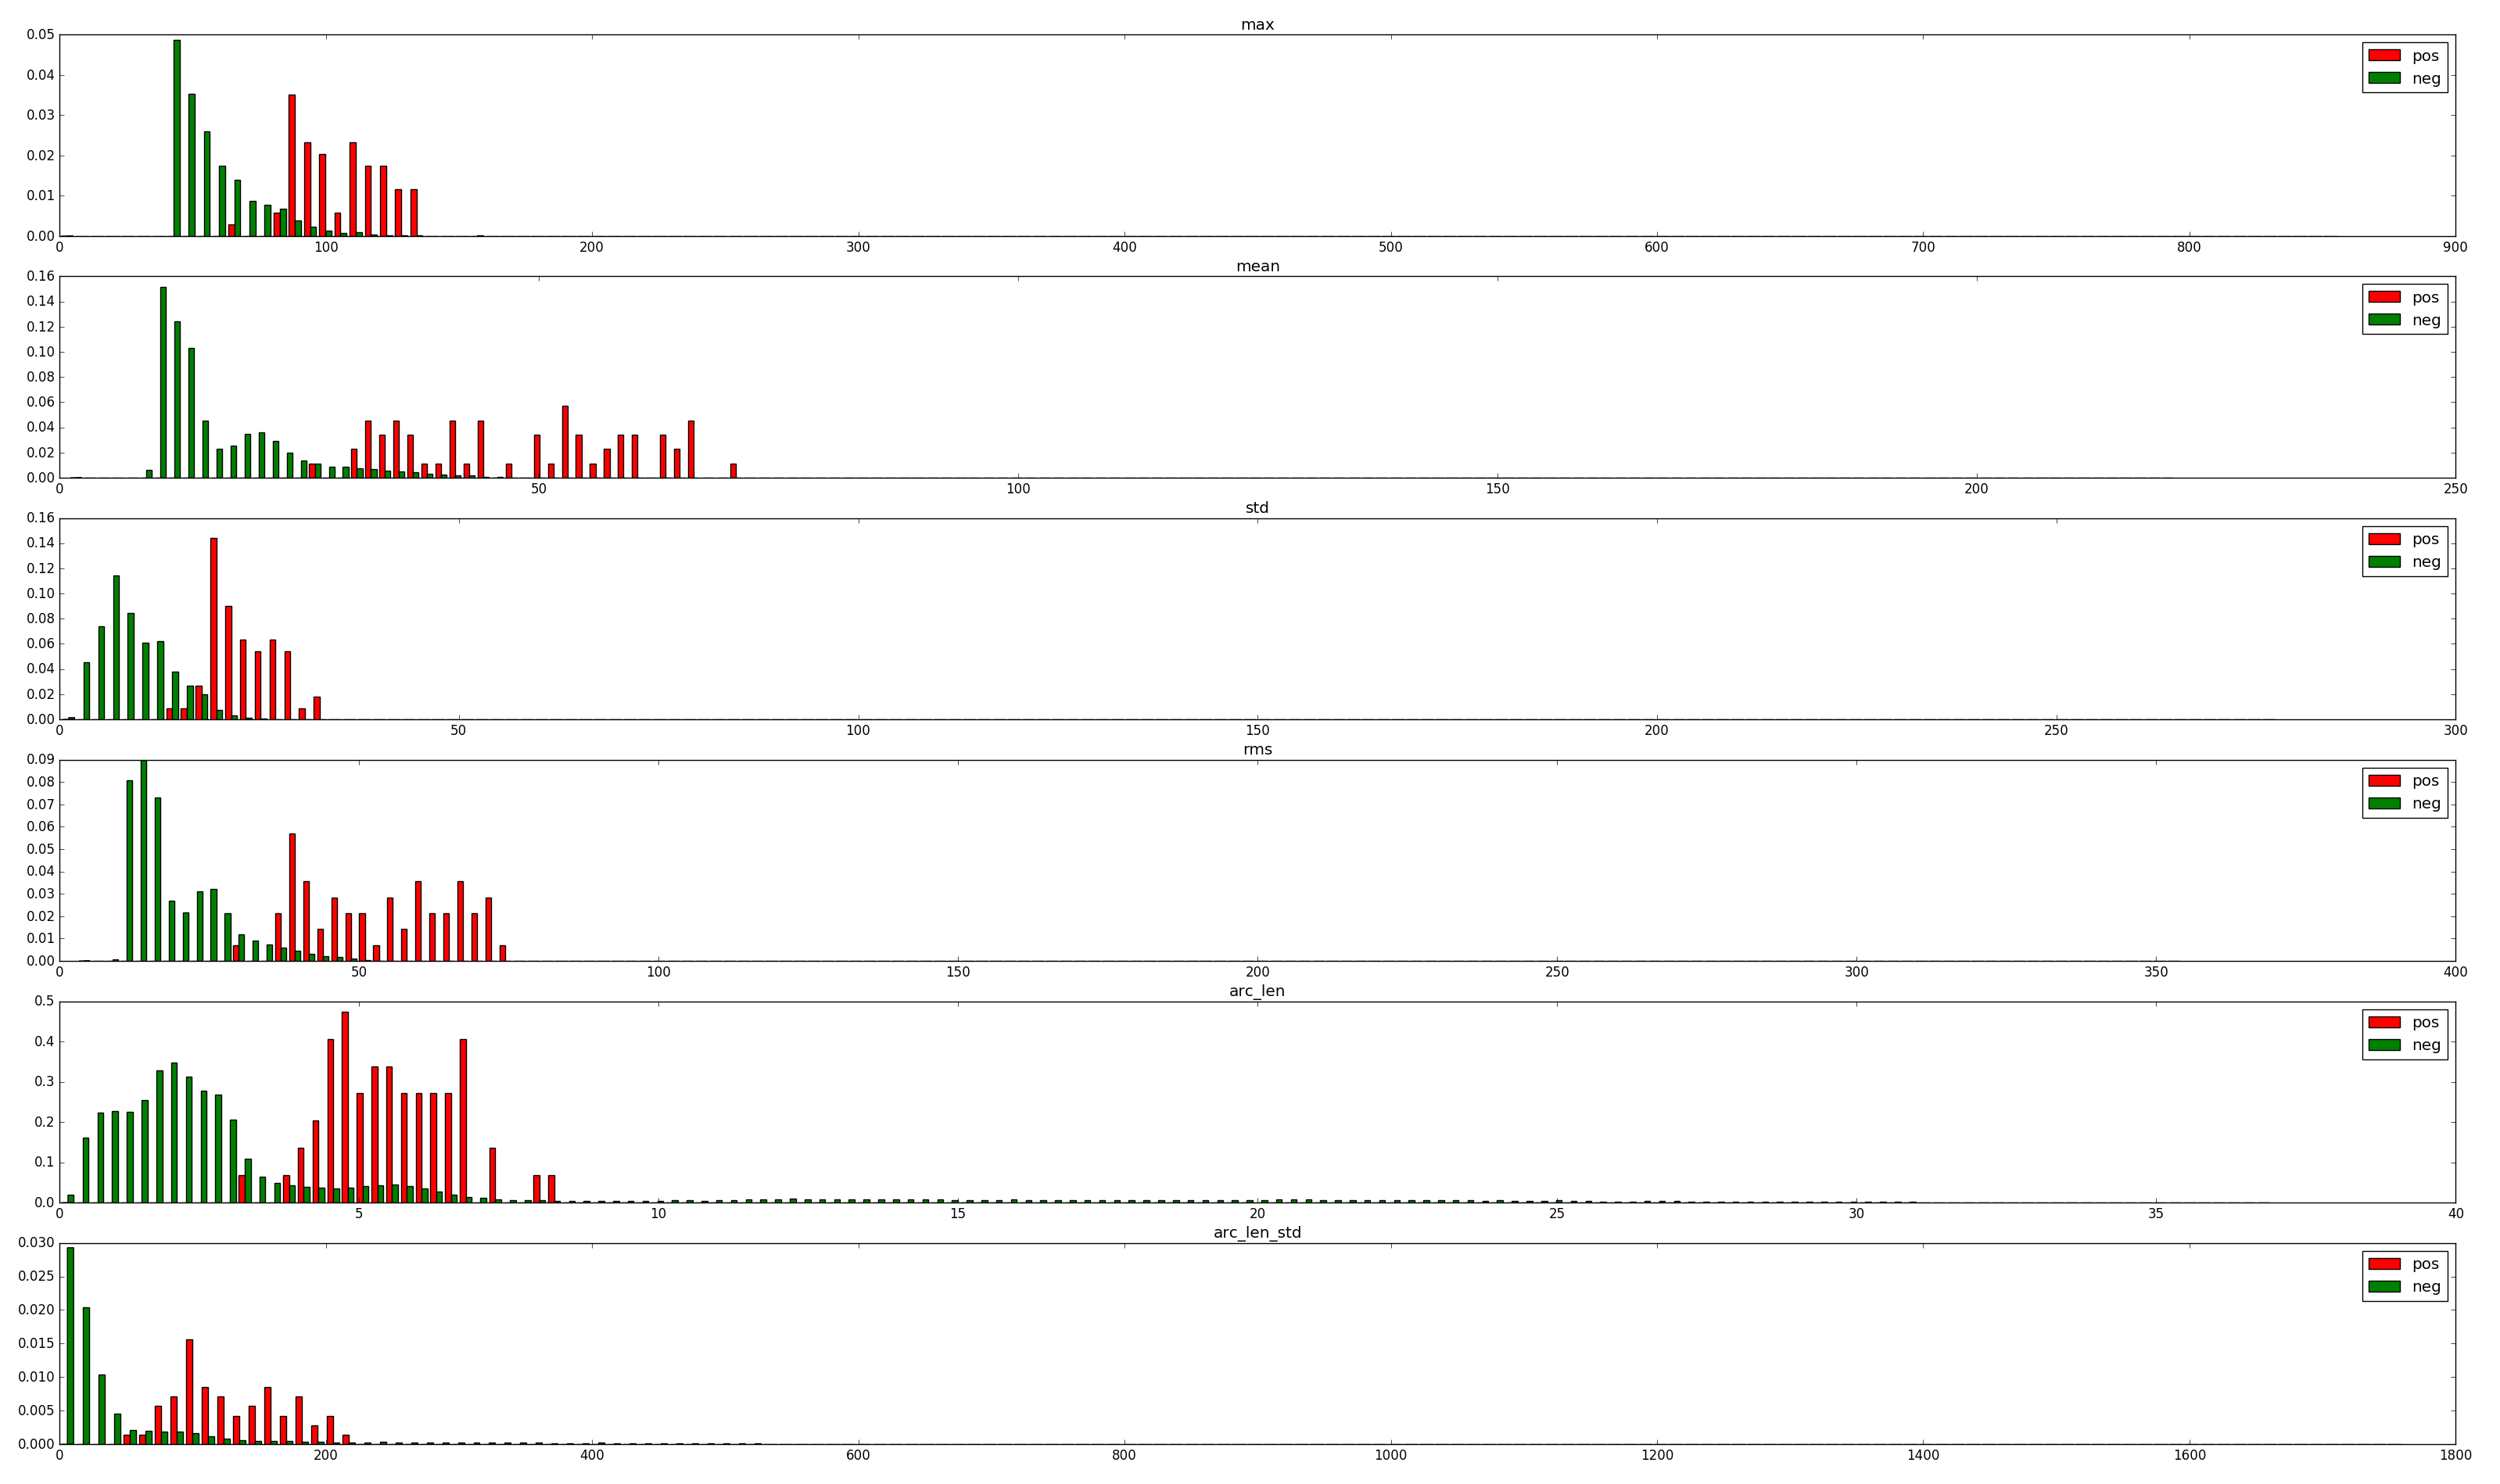
\includegraphics[width=\columnwidth]{hist_features_after_win_size_1_2.png}
\caption{Histogram of feature values in the 2-second window after the~$40 m/s^2$ spike.}
\label{fig:afterhist}
\end{minipage}
\end{figure*}

% \begin{figure*}[t]
% \begin{center}
% 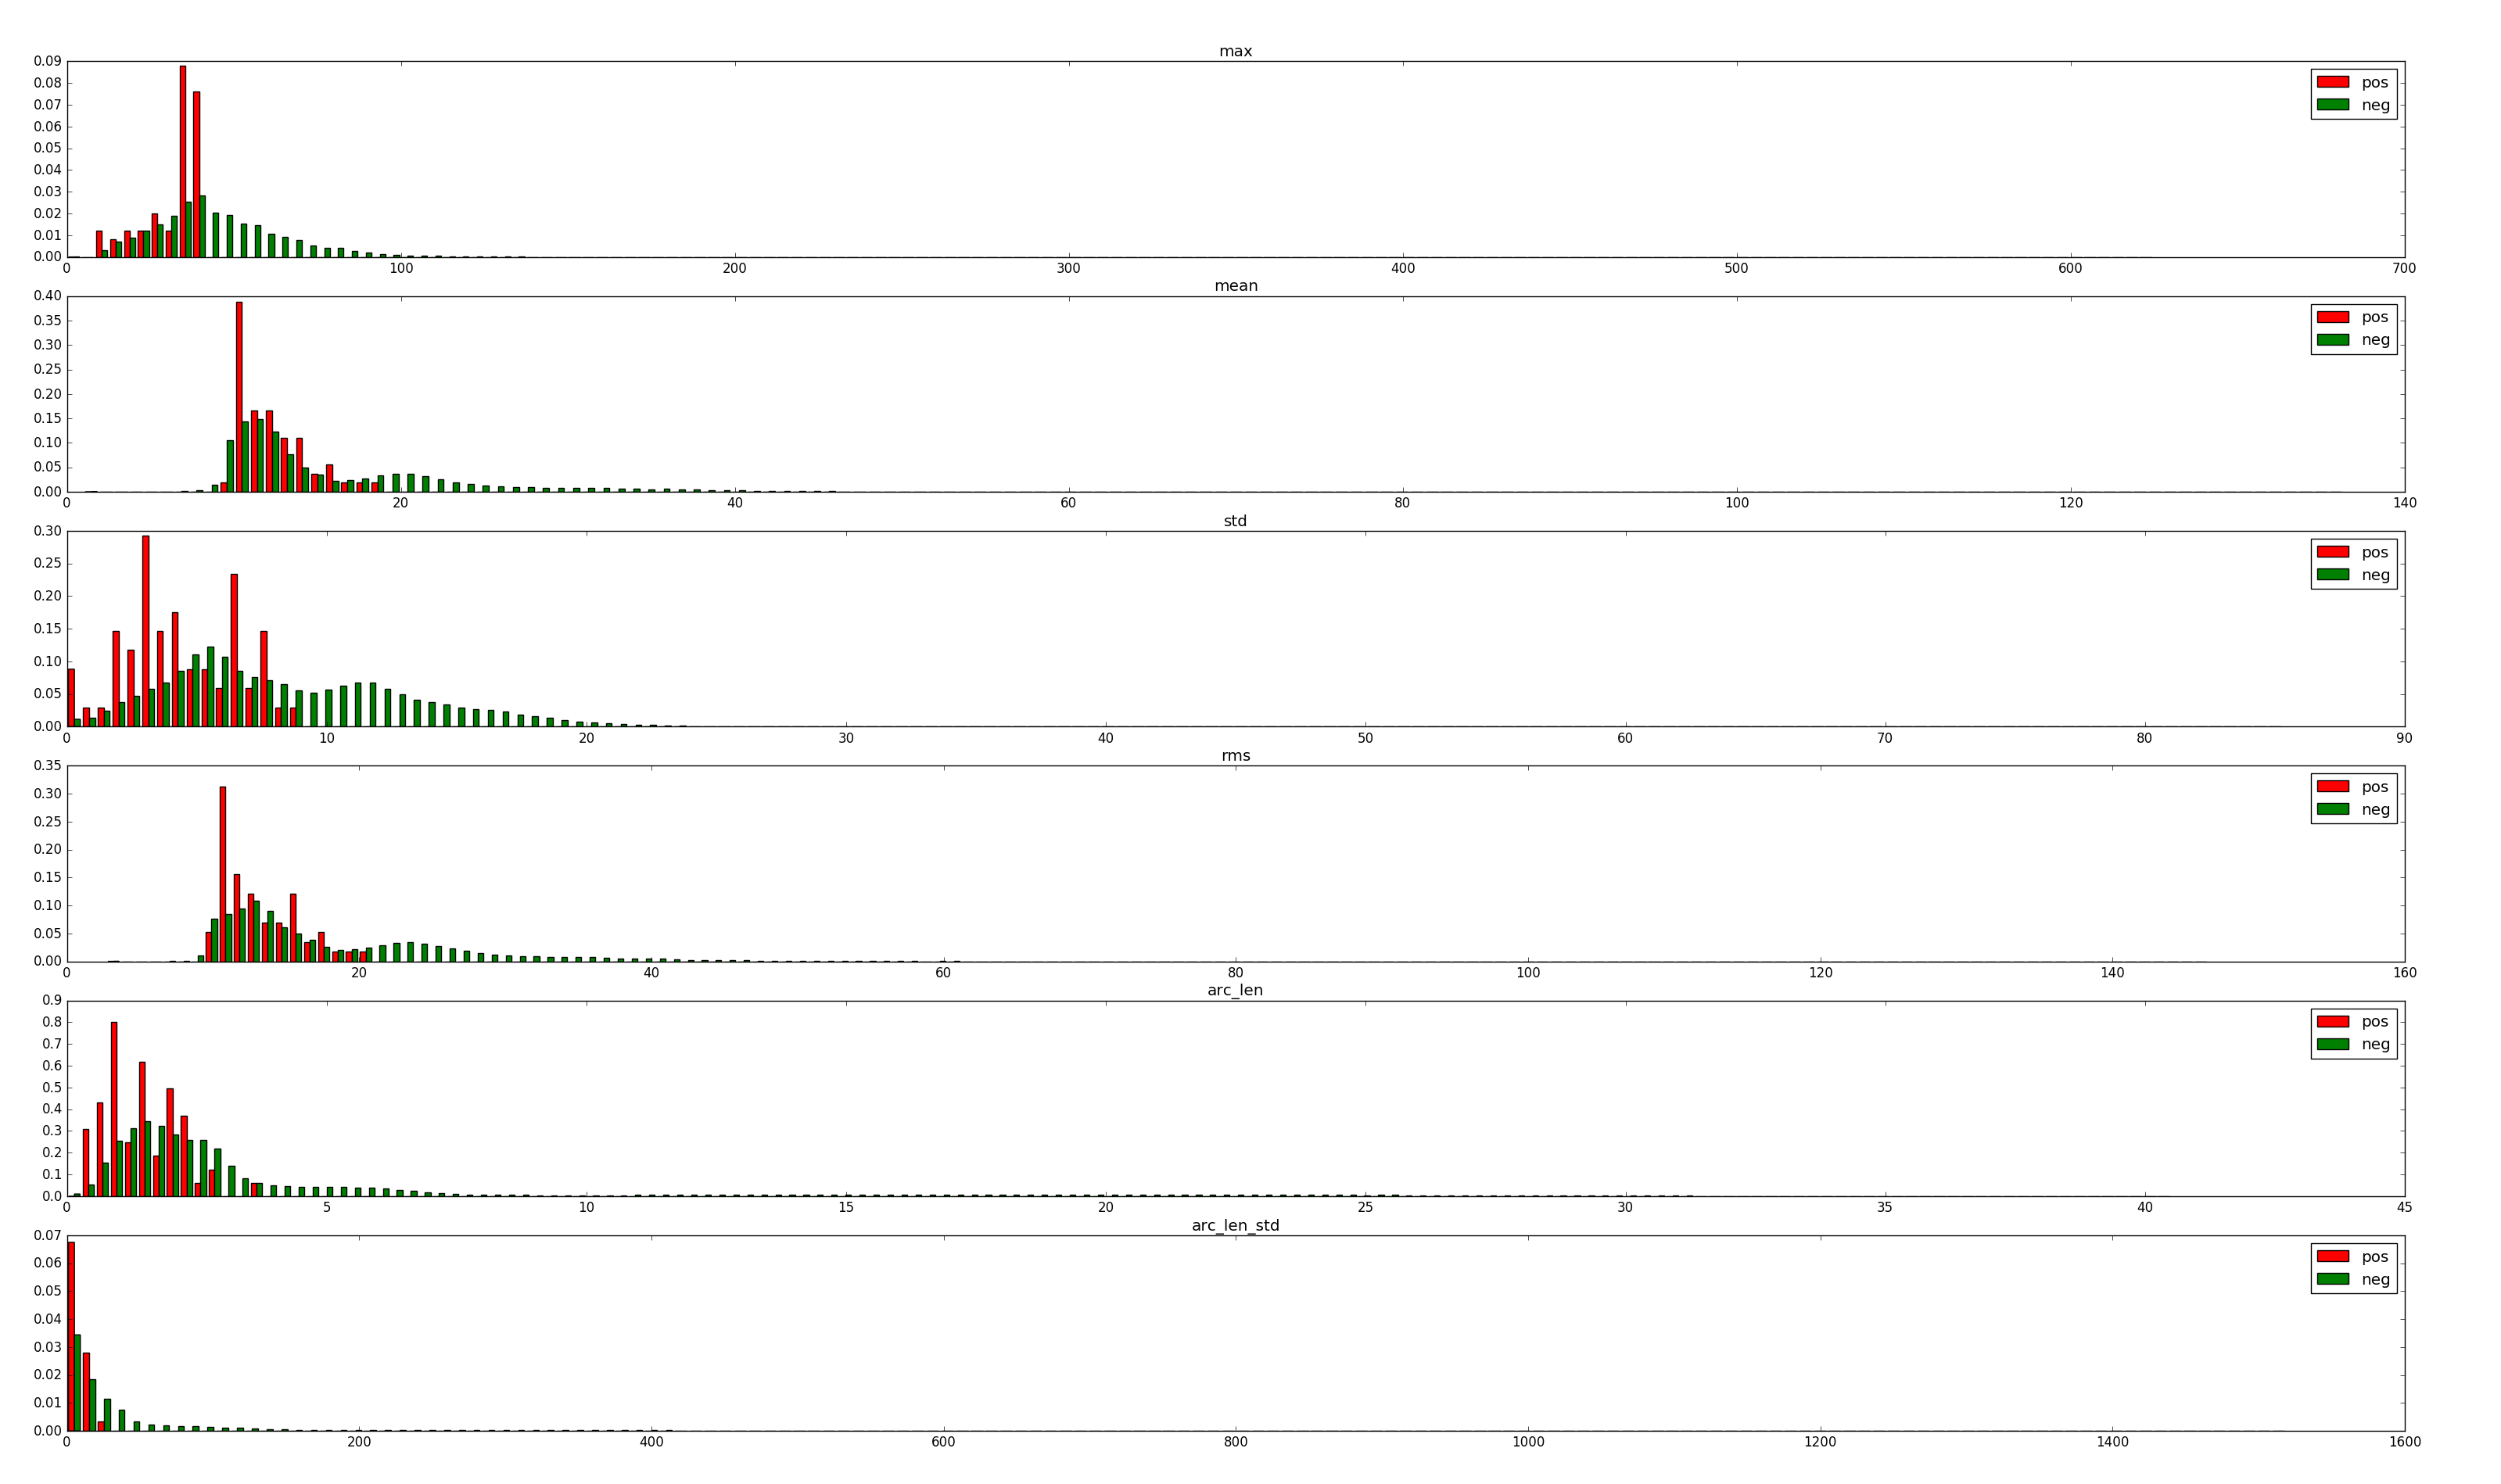
\includegraphics[width=\textwidth]{hist_features_before_win_size_1_2.png}
% \end{center}
% \caption{Histogram for each of the 6 features for the 1-second window before the~$40 m/s^2$ spike.  The features are listed in the order presented in Section~\ref{s:features}, e.g., the top histogram is for the maximum.  Red bars indicate thefts, and green bars indicate non-theft windows.}
% \label{fig:beforehist}
% \end{figure*}

% \begin{figure*}[t]
% \begin{center}
% 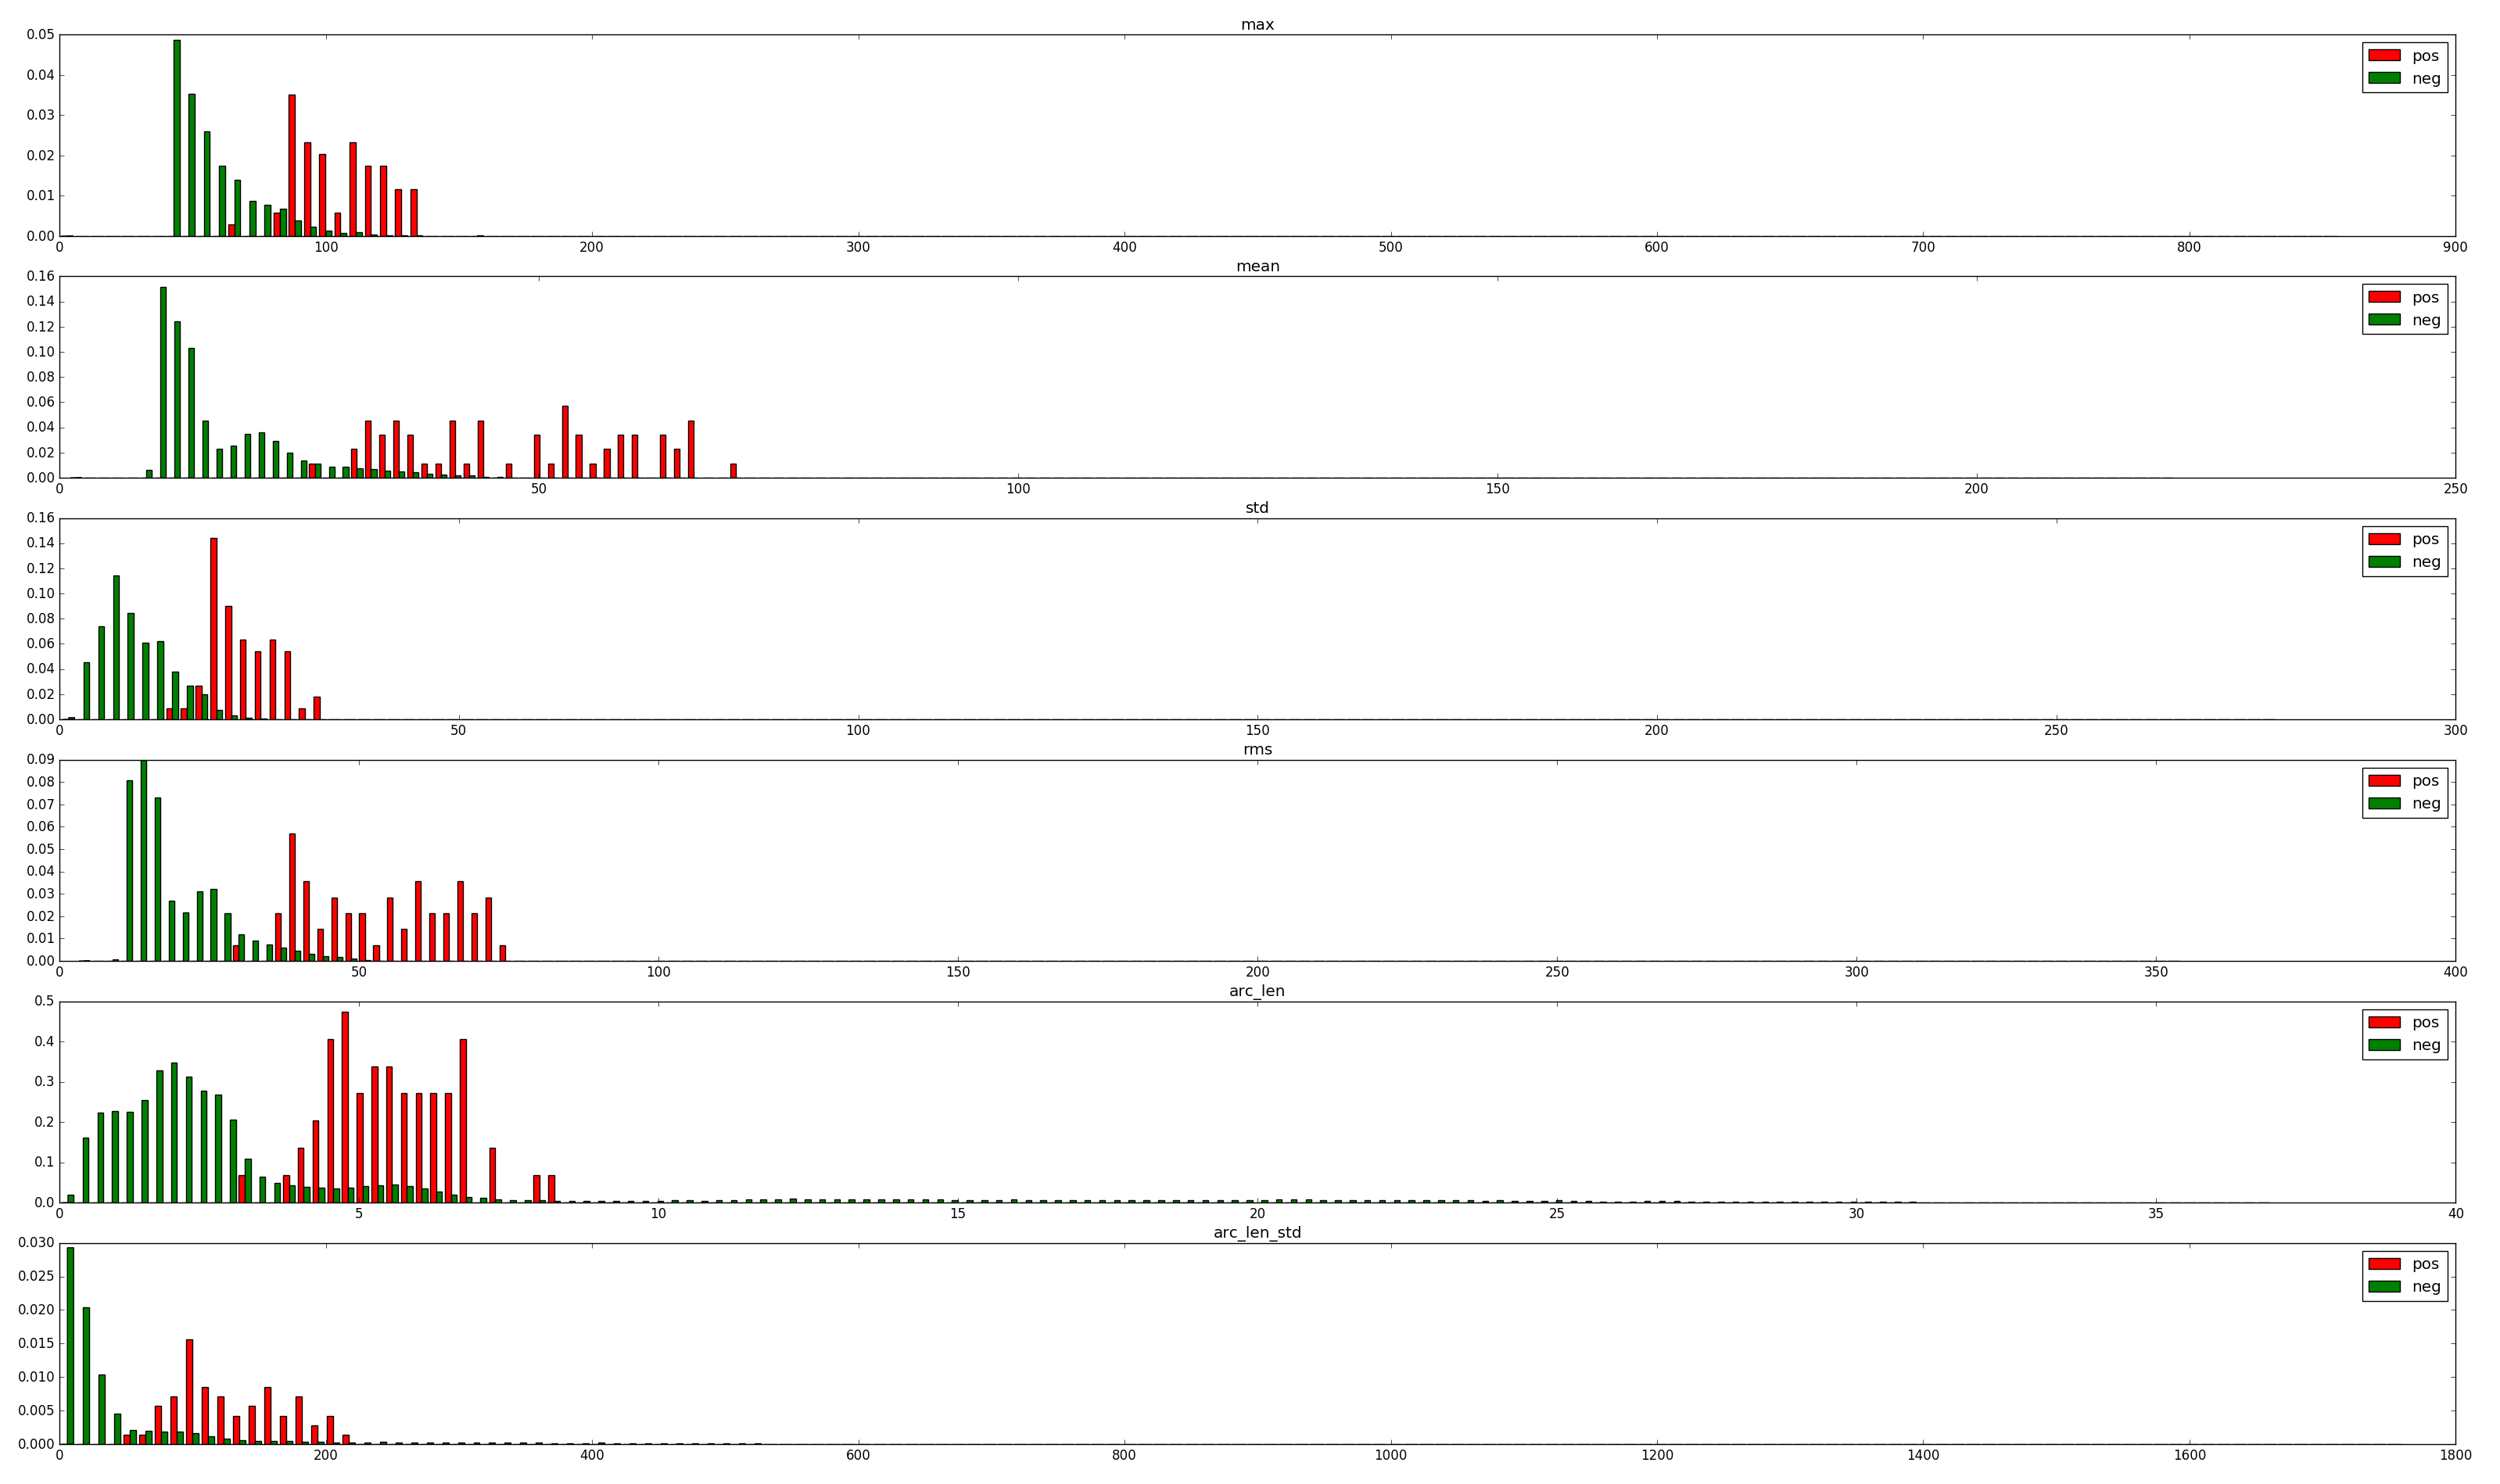
\includegraphics[width=\textwidth]{hist_features_after_win_size_1_2.png}
% \end{center}
% \caption{Histogram of feature values in the 2-second window after the~$40 m/s^2$ spike.}
% \label{fig:afterhist}
% \end{figure*}

To compare the performance of random forests and logistic regression, we fine tuned the class weights for the logistic regression classifier to lower its true positive rate until it is approximately the same as the random forests classifier, then we compared the number of false positive instances of the two classifiers.
We find that logistic regression has 14 false positive instances at a 67\% true positive rate (25 true positive instances),
while random forests has 15 false positive instances at a 62\% true positive rate (23 true positive instances).
Thus the performance of the two classifiers seems comparable in this regime.
The advantage of logistic regression is that we found adjusting class weights was more effective at controlling the false-positive/false-negative tradeoff for the logistic regression classifier.
The Receiver Operating Characteristic (ROC) curves for the logistic regression and random forests classifiers are shown in Figure~\ref{fig:roc}.

\begin{figure}[t]
\begin{center}
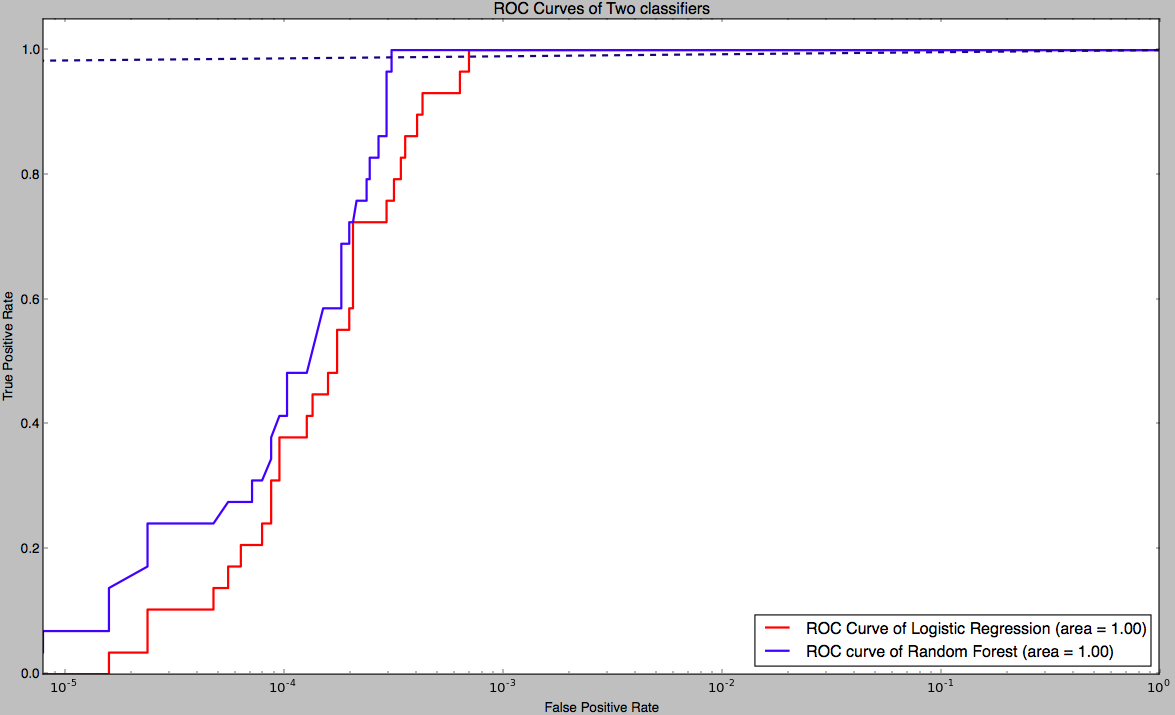
\includegraphics[width=1.0\columnwidth]{roc_curves_log_line.png}
\end{center}
\caption{ROC curves of logistic regression and random forests. The x-axis is in logarithmic scale.}
\label{fig:roc}
\end{figure}



% \section{Related Work}

Many researchers have studied using smartphone sensors for continuous user authentication.
The benefit of continuous user authentication is that it happens unobtrusively, without requiring any action from users.
Continuous authentication could serve as a mitigation for theft: if the phone can detect rapidly enough that it is no longer being used by the rightful owner, it could lock itself to prevent the thief from accessing sensitive data on the phone. 

One approach is to use smartphone accelerometer data for gait recognition.
These systems often extract some features from the sensor data and then apply machine learning.
Derawi et~al.\ achieved an equal error rate of 20\%~\cite{derawi:gait}.
``Equal error rate'' is a measure of accuracy where the system is tuned so the false accept rate and false reject rates are equal, and then that error rate is reported.
Primo et~al.\ show that accelerometer-based gait authentication is somewhat dependent on the position in which the phone is held, which is a challenge for deploying gait authentication outside of a laboratory environment~\cite{primo:context}. 
They showed how to infer the position of the phone (in the person's hand vs.\ in a pocket) with 85\% accuracy, and they showed how to use this information to increase the accuracy of user authentication to 70--80\%.
They do not report performance as equal error rate.
Juefei-Xu et~al.\ show that the pace at which people walk also affects the sensor readings, and it is possible to improve accuracy by first identifying the pace at which the user is walking, then using a model tailored towards that pace~\cite{xu:pace}.
Their system achieved an equal error rate of 4--8\% (depending on the pace); or a false reject rate of 0.5--5\% at a false accept rate of 0.1\%.
Kwapisz et~al.\ generalized gait authentication to cover not just walking but also jogging and ascending and descending stairs~\cite{kwapisz:biometrics} and
achieved false reject rates of 10--15\% at a false accept rate of about 5\%.

It is not clear whether gait recognition is sufficient on its own for deployable user authentication.
One limitation is that it can only attempt to authenticate the user while the user is walking; when the user is still, it cannot infer user identity.
Another limitation is that the error rate is still fairly high: if the classifier is run continuously, once per second, even a false reject rate as low as 0.5\% will cause hundreds or thousands of false rejections per week.
Thus, gait recognition might need to be combined with other methods to yield a deployable defense against theft.

Our work builds on the methods previous researchers have used to process sensor data and extract features.
The accelerometer sensor provides raw data in the form of $X,Y,Z$ accelerations; it is useful to also compute the magnitude $M=\sqrt{X^2+Y^2+Z^2}$ of the acceleration, as that is independent of the direction of the acceleration.
Prior papers have used several methods for cleaning the raw accelerometer data, including interpolation and re-sampling to deal with irregularly sampled data and a weighted moving average filter to mitigate sensor noise.
These schemes typically divide the resulting time series into windows, each window containing about a second of sensor data.
For instance, Primo et~al.\ used overlapping windows, with each window containing 100 samples and having an overlap of 50 samples with the next window; Derawi et~al.\ and Juefei-Xu et~al.\ used non-overlapping windows, which were about 1 second in width.
Derawi et~al.\ and Juefei-Xu et~al.\ used the sensor readings as the features, while Primo et~al.\ and Kwapisz et~al.\ computed hand-crafted features from the readings, where each feature records a summary statistic on the sensor readings in the window (e.g., mean, minimum, maximum, standard deviation, number of zero crossings, etc.).

Feng et~al.\ investigated using the unique way the user picks up their phone as a biometric for user authentication~\cite{feng:pickup}. 
They achieved an equal error rate of 6--7\%.
They used the smartphone accelerometer, gyroscope, and magnetometer; in our work, we avoid the gyroscope sensor, as its power consumption is significantly higher than the accelerometer, and therefore is currently not a practical solution for continuous authentication.

Mare et~al.\ developed a continuous authentication system where the user wears a smartwatch or bracelet, which is used to authenticate the user to their computer~\cite{mare:zebra}. 
Their continuous authentication scheme works well and could plausibly be used to authenticate to a smartphone, but it requires users to wear a bracelet; in contrast, we seek solutions that do not require the user to carry or wear any additional devices.

The most closely related work is by Chang et~al.\, who used the way
that each person takes their phone out of their bag or pocket as a 
form of biometric authentication~\cite{cheng:theft}.
They use accelerometer and gyroscope data to detect when the user picks
up their phone, and then they apply dynamic time warping and boosting to
determine whether the pickup motion matches known templates from the
owner of the phone.
Their system achieves a 10\% false positive rate and a 5.5\% false negative rate, which are relatively high,
considering that users may pick up their phones dozens of times each day.

The prior work focuses on authenticating the user.
In contrast, we take a different approach: we attempt to detect the
specific motion pattern that occurs during a grab-and-run or pickpocket theft.
The benefit of biometric authentication is that it provides a comprehensive
way to detect theft, regardless of the way the phone was stolen; however,
as summarized above, the false positive rates of existing schemes
are fairly high.
Our scheme is limited to detecting a particular type of theft, but achieves
far lower false positive rates.
Our classifier is also user-independent and does not require obtaining
training data from each user; we use the same classifier for all users.




\section{Methodology}

In this section, we describe the data collection software, which we used to gather positive and negative data for our training and test sets as well as the feature extraction scheme, and other classifier design decisions.

\subsection{Data Collection}

\subsubsection{Software}
We used an Android application to record data from the smartphone's 3-axis accelerometer, which then encrypted it and stored it in the cloud.
We acquired sensor data at the highest sampling rate supported by the phone using SENSOR\_DELAY\_\\FASTEST~\cite{android:doc}. 
On most devices, including the one we used for the simulated theft experiment, the sampling rate is 100 Hz. 

\subsubsection{Simulated Theft Experiment}
Because data from real thefts is hard to obtain, we simulated three types of common smartphone theft scenarios, based on campus police alerts that we receive, with one researcher acting as a smartphone user and another one playing the role of a thief. 
The three theft scenarios are as follows:
\begin{enumerate}
\item The user stands still and holds the phone with one hand as she is using the device, for instance reading a text; the thief approaches from behind, grabs the phone with both hands and runs away in the forward direction. 
\item The user holds the phone in front of her with one hand while walking at a constant speed; the thief approaches from behind, grabs the phone with both hands and runs away in the forward direction. 
\item The third scenario simulates pick-pocket thefts. The user places the phone in the back pocket of their pants and stands still; the thief approaches from behind, steals the phone from user's pocket and runs away in the forward direction.
\end{enumerate}
We collect 40 instances of each scenario, for a total of 120 trials. 
Data collection was split across four sessions, each consisting of 10 trials per scenario, with different researchers acting as the victim and thief in these two sessions. 
We ran the experiment on flat ground in an open space, so the experiment was not interrupted. 
We also made sure that the thief ran at least 40 feet after gaining possession of the victim's phone.
We used a Nexus 5X smartphone (InvenSense MPU6515 embedded accelerometer) with Android version 7.1.1 for data collection in our simulated theft experiment.
Figure~\ref{fig:simtheft} plots one example of accelerometer readings from a single simulated theft.


\begin{figure}[t]
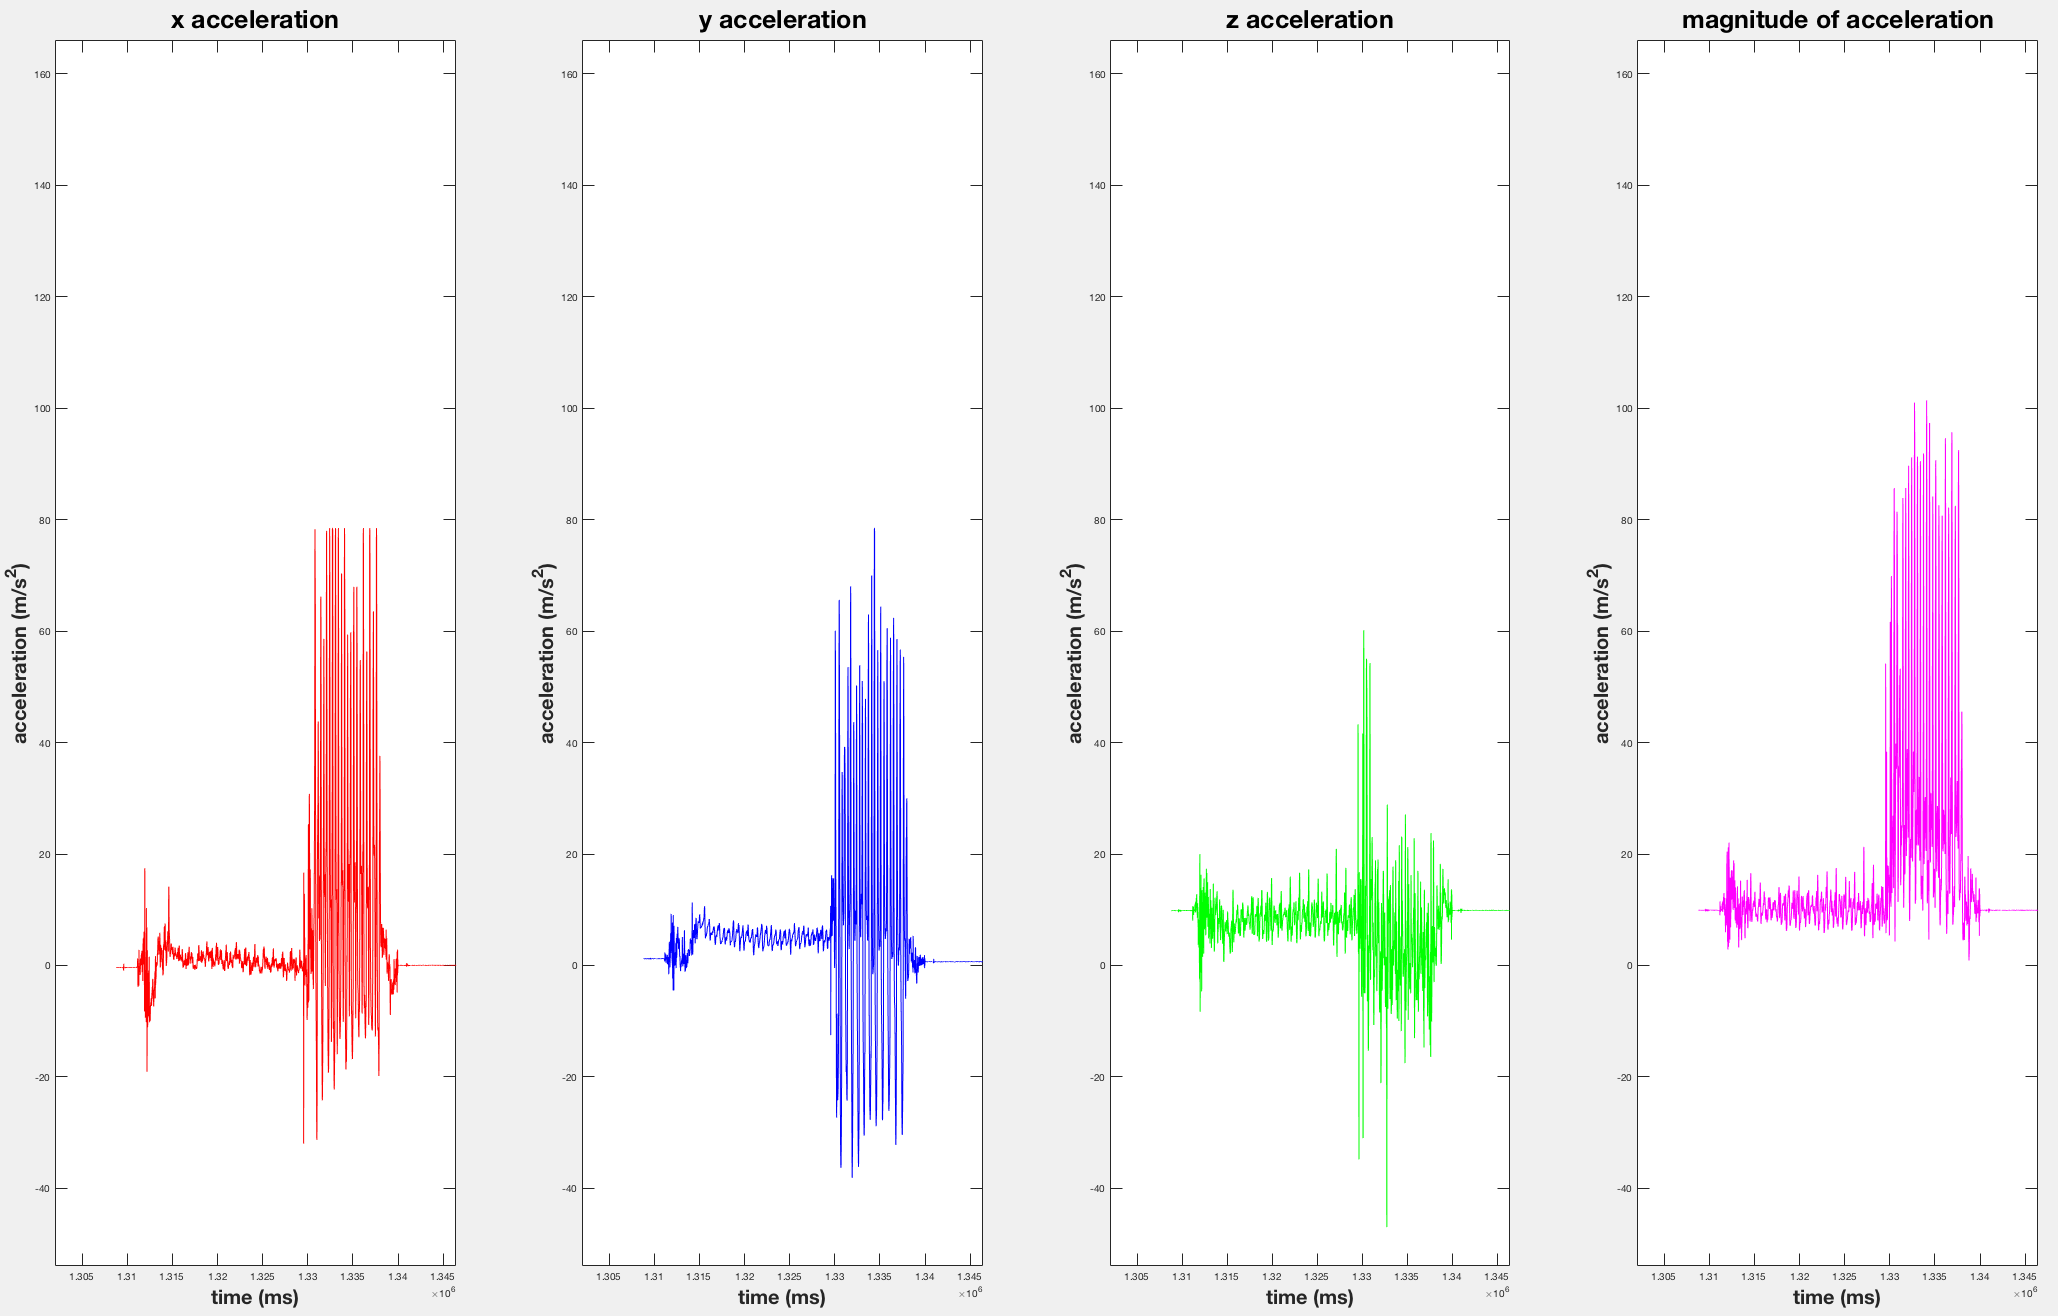
\includegraphics[width=1.0\columnwidth]{pos_acc_separated.png}
\caption{The X, Y, Z and magnitude of acceleration, respectively, from one simulated theft instance.}
\label{fig:simtheft}
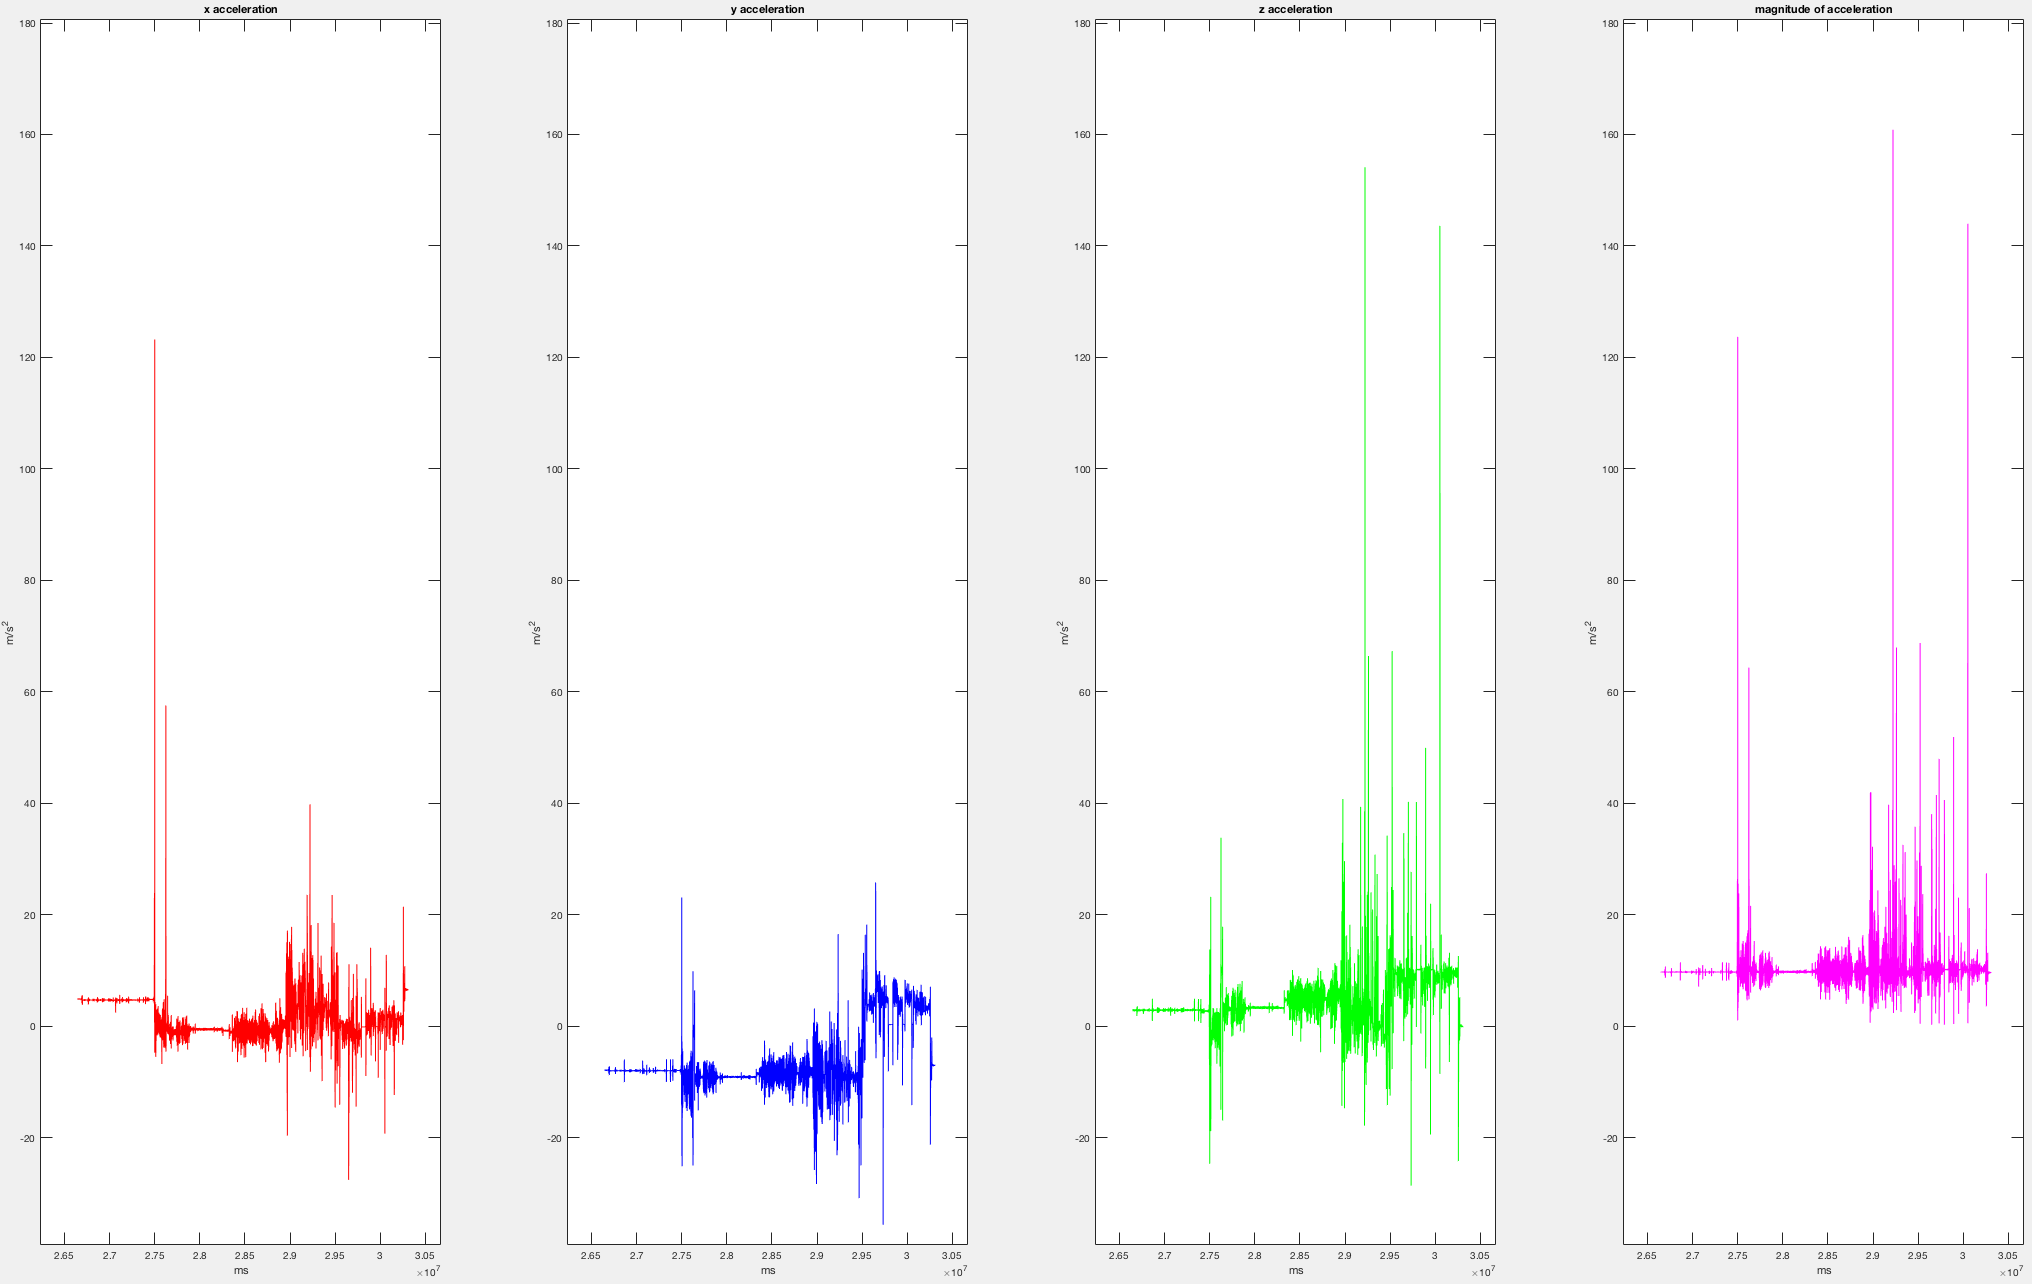
\includegraphics[width=1.0\columnwidth]{neg_acc_separated.png}
\caption{The X, Y, Z and magnitude of acceleration, respectively, during normal usage at an arbitrary time period.}
\end{figure}




\subsubsection{Field Study}
We performed a field study to gather data from ordinary smartphone users while they perform everyday activities, including walking, running, driving, possibly excercising, and anything else that occurred during their lives over the field study period.
% We obtained approval from the University of California, Berkeley IRB (Institutional Review Board) for this study. 
We obtained approval from our university IRB for this study. 
The study was conducted in a metropolitan area from September to December 2016.
% The study was conducted in the Bay Area of the United States from September to December 2016.
None of the participants experienced a phone theft during the study interval,
so we were able to use the accelerometer data collected from the user study as negative samples for our machine learning algorithms (i.e., instances of non-theft activity).

We posted a recruitment advertisement on Craigslist in September 2016. 
% We posted a recruitment advertisement on the Craigslist under the SF Bay Area `jobs et cetera' category in September 2016. 
We only recruited participants who used an Android smartphone with version 5.0 and above. 
After obtaining their consent, we installed our data collection application on their phones and collected data for a three-week period.
The application ran in the background and collected accelerometer sensor readings continuously, 24 hours a day.
We contacted participants weekly to make sure their phones were functioning correctly and troubleshoot any data collection issues.
Each participant was paid \$150 for their participation.

The study was divided across 3 rounds; each round lasted 3 consecutive weeks. 
A total of 55 participants were recruited, and
53 out of the 55 subjects completed the study. 
In the first round, 2 of the 18 participants did not complete the study.
Detailed demographic information about the participants of this user study is listed in Table~\ref{tbl:demographics}.
In aggregate, they used 21 different smartphone models from 6 different manufacturers and 8 different Adroid versions. This ensures the dataset containing diverse devices, and the classifiers are not specific to a particular type of smartphone or Adroid version.
We also asked participants how they typically carried their phone, when it was not in their hands; 33 reported keeping it in their pockets, 9 in their purses, 12 in multiple locations (e.g., pocket or purse, pocket or backpack), and 1 did not respond.
During the study, the subjects carried their phones while performing daily activities, for example walking, driving, running and possibly excercising. Data from a wide variety of real-world activities ensures the generability of the classifiers trained on it. 

\begin{table}[H]
\centering
\begin{tabular}{rrrrrr}
\hline
      & Male & Female & Age 20--29 & 30--39 & 40+ \\ \hline
R1    & 5    & 11     & 8         & 6     & 2   \\
R2    & 10   & 8      & 7         & 7     & 4   \\
R3    & 11   & 8      & 9         & 4     & 6   \\
Total & 26   & 27     & 24        & 17    & 12  \\ \hline
\end{tabular}
\caption{Participants' demographic information.}
\label{tbl:demographics}
\end{table}




\subsection{Feature Extraction}
\label{s:features}

Our theft scenarios all involved a sudden movement of the phone, which causes a large acceleration.
Therefore, as a first filtering step, we filtered the data to focus on times near when a large motion occurs.
In particular, our classifier is activated when the magnitude of acceleration $M$ exceeds~$40 m/s^2$.
We extract a one-second window before the activation time and a $n$-second window after the activation time, compute features on each of these windows, and use them for classification.
We vary $n$ from 1 to 7 to obtain the best classification accuracy.
We chose a threshold of~$40 m/s^2$ as all of our simulated thefts experienced accelerations exceeding that threshold when the phone was initially grabbed by the thief.

We first identified 16 candidate features, 8 features for each of the two windows.
In particular, we computed the minimum, maximum, mean, standard deviation, root mean square, arc length, product of arc length and standard deviation, and mean absolute value, each computed on the magnitude values ($M$) within the window.
We chose to only compute these features on the magnitude of the acceleration, and not the $X$, $Y$, and $Z$ components, because the magnitude is non-directional and thus more robust to changes in the orientation of the phone. 
We then visualized the distribution of these features for the two classes and applied feature selection techniques to choose a subset of features that yield good performance.
We removed the minimum and mean absolute value from the feature list because removing them did not affect the performance of the classifiers. 
As a result, we extract a 12-dimensional feature vector, 6 features from the before-window and 6 from the after-window, every time the detector is triggered.

Let $M_1,\dots,M_k$ denote the time series of acceleration magnitudes within the window.
The features are computed as follows:
\begin{itemize}
\item \emph{Maximum}: the maximum value of the magnitude within the window, i.e., $\max(M_1,\dots,M_k)$.
\item \emph{Mean}: the average value of magnitude in a window, i.e., $(M_1+\dots + M_k)/k$.
\item \emph{Standard deviation}: the standard deviation of magnitude values in a window.
\item \emph{Root mean square}: the RMS of magnitude values in a window, i.e., $(M_1^2 + \dots + M_k^2)^{1/2}/k^{1/2}$.
\item \emph{Arc length}: the average of the absolute differences between all adjacent magnitude values in a window, i.e., $(|M_2-M_1| + |M_3-M_2| + \dots + |M_k-M_{k-1}|)/(k-1)$.
Intuitively, this captures the average of the first derivative of the acceleration.
\item \emph{Product of arc length and standard deviation}: the product of the two feature values.
\end{itemize}

Because the accelerometer sensor reports readings in the same units on all Android phones, and because our features are relatively simple, we believe these features capture fundamental, device-independent characteristics of the motion rather than anything specific to the particular device used for data capture (e.g., in contrast to the hardware-based differences documented by Dey et al.~\cite{Dey2014}).

We obtained 60 positive instances from the 60 simulated thefts.
After applying the~$40 m/s^2$ threshold, we obtained approximately approximately 248,000 negative samples from the data collected in the field study. 
We then applied boolean classification techniques to this data set.


% \begin{figure}[t]
% 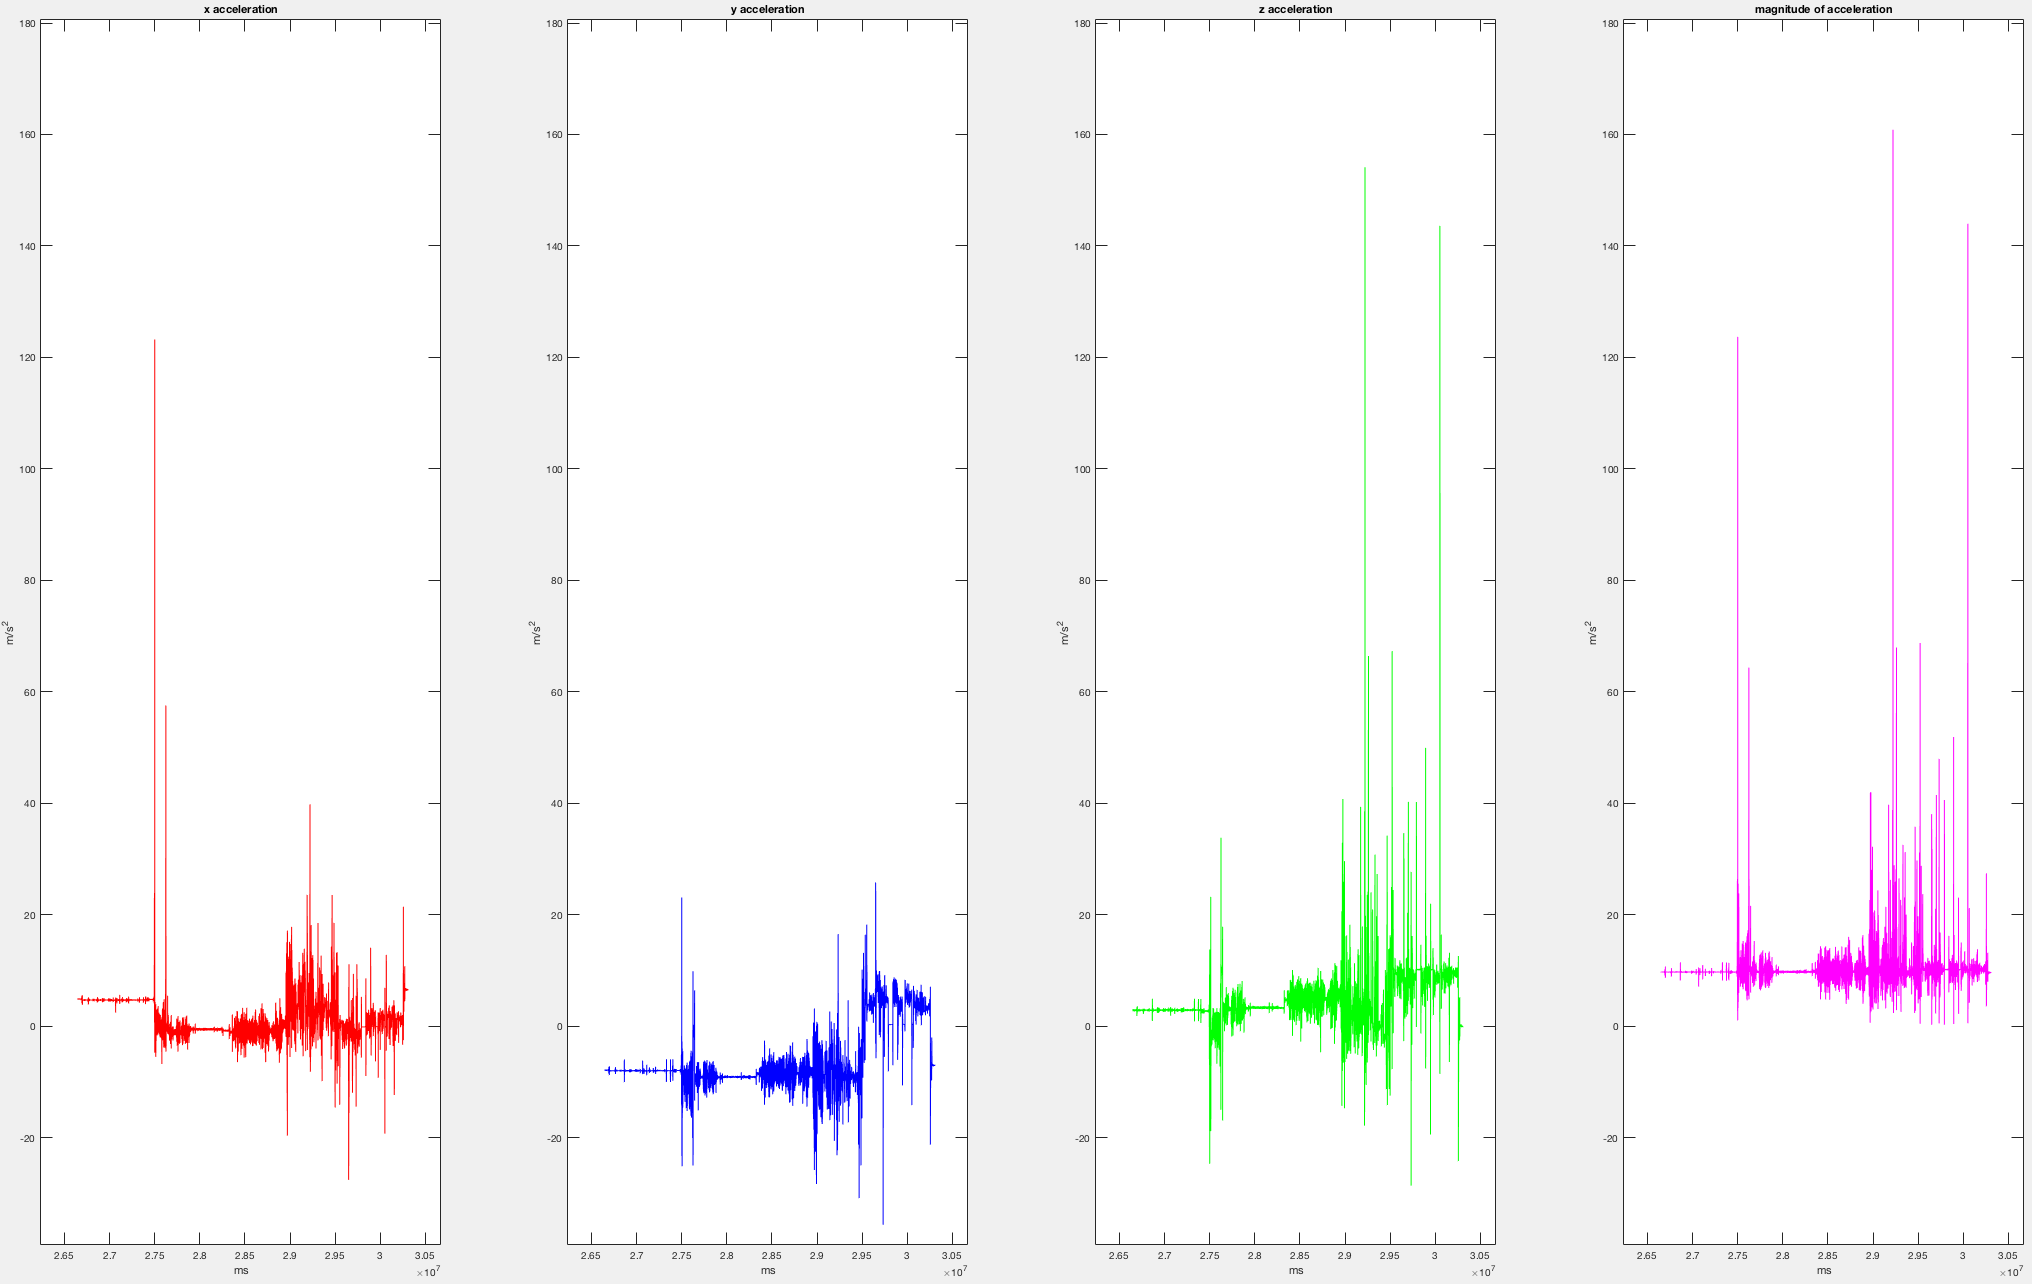
\includegraphics[width=1.0\columnwidth]{neg_acc_separated.png}
% \caption{The X, Y, Z and magnitude of acceleration, respectively, during normal usage at an arbitrary time period.}
% \end{figure}



\subsection{Machine Learning Algorithms}
We evaluate three standard machine learning algorithms: linear SVM, logistic regression and random forests.
Because we have many more negative samples than positive ones, we tried different settings for class weights to weight positive instances more highly than negative ones.
We also evaluated different window sizes for the after-window.
We found that a 2-second after-window yielded better accuracy than a 1-second after-window since 2-second windows encapsulate more complete acceleration information about the motions, and larger window sizes did not offer much improvement.
Therefore, all of our experiments use a 1-second before-window and a 2-second after-window.
We partitioned the entire dataset, which consists of 120 positive samples and approximately 248,000 negative samples, into training and test sets with 7:3 ratio.
Then we trained the classifiers on the training set and reported the predition results of the test set.



\section{Results}
Among the three classifiers, logistic regression performs the best.
Confusion matrices for logistic regression, random forests, and a linear SVM
are shown in Table~\ref{fig:cmat}.
The logistic regression classifier has a false positive rate of 0.09\%. Given that the field study involved 53*3=159 person-week of data, and the logistis regression would report 248,000*0.09\%=223 false positives, the total number of samples extracted from the field study data times the false positive rate. This means that on average users receive 223/159$\approx$1.4 false alarm every week, and a true positive rate of 100\%.
The random forests classifier has an even lower false positive rate (approximately one false alarm per month),
but it only detects 60\% of the thefts.

Only a small fraction of predicted positives will actually be theft, but we expect this will be acceptable due to the relatively low cost of false positives: it means users will have to unlock their phones one extra time per week, which seems likely to be tolerable. We report the false positive rate rather than precision, because the false positive rate is easily interpretable and not sensitive to the rate at which theft occurs. The precision is sensitive to the number of simulated thefts included in the dataset, which might not match the number of actual thefts that are likely to occur over a given period of time.


\begin{table}[t]
\centering
\begin{tabular}{@{}lll@{}}
\toprule
              & Predicted Negative & Predicted Positive \\ \midrule
True Negative & 74446              & 72                 \\
True Positive & 0                  & 37                 \\ \bottomrule
\end{tabular}

\begin{tabular}{@{}lll@{}}
\toprule
              & Predicted Negative & Predicted Positive \\ \midrule
True Negative & 74503              & 15                 \\
True Positive & 14                 & 23                 \\ \bottomrule
\end{tabular}

\begin{tabular}{@{}lll@{}}
\toprule
              & Predicted Negative & Predicted Positive \\ \midrule
True Negative & 74501              & 17               \\
True Positive & 17                 & 20                 \\ \bottomrule
\end{tabular}
\caption{Confusion matrices for a logistic regression classifier (at top; with class weights 1:200), random forests classifier (middle; class weights 1:5000), and a linear SVM classifier (bottom; class weights 1:1000).}
\label{fig:cmat}
\end{table}

% \begin{table}[t]
% \centering
% \begin{tabular}{@{}lll@{}}
% \toprule
%               & Predicted Negative & Predicted Positive \\ \midrule
% True Negative & 248223             & 170                \\
% True Positive & 0                  & 60                 \\ \bottomrule
% \end{tabular}
% \caption{Confusion matrix for a logistic regression classifier trained
% with class weights set to 1:200.}
% \label{fig:logistic}
% \end{table}

% \begin{table}[t]
% \centering
% \begin{tabular}{@{}lll@{}}
% \toprule
%               & Predicted Negative & Predicted Positive \\ \midrule
% True Negative & 248360             & 33                 \\
% True Positive & 32                 & 28                 \\ \bottomrule
% \end{tabular}
% \caption{Confusion matrix for a random forests classifier trained with
% class weights set to 1:5000.}
% \label{fig:rf}

% \end{table}

% \begin{table}[t]
% \centering
% \begin{tabular}{@{}lll@{}}
% \toprule
%               & Predicted Negative & Predicted Positive \\ \midrule
% True Negative & 246522             & 1871               \\
% True Positive & 42                 & 18                 \\ \bottomrule
% \end{tabular}
% \caption{Confusion matrix for a linear SVM classifier trained with
% class weights set to 1:1000.}
% \label{fig:svm}
% \end{table}


To get a better understanding of why our classifier is successful,
we computed feature rankings to find the most predictive features.
For logistic regression, we used standardized coefficients as the feature importance score:
the score for feature $i$ is $|\alpha_i| \cdot \sigma_i$, where $\alpha_i$ is the coefficient for feature $i$ in the logistic regression model and $\sigma_i$ is the standard deviation of feature $i$ in the training set.
In addition, we computed the 95\% confidence intervals for all standardized coefficents using 50 epoches of the entire data set.
The feature importance scores and their 95\% confidence intervals for the logistic regression classifier are listed in Table~\ref{tbl:importance-lr}.
The most discriminative features are
the maximum of the before-window,
the product of arc length and standard deviation of the after-window,
and the arc length of the before-window.
Plotting a histogram of feature values (see Figures~\ref{fig:beforehist} and \ref{fig:afterhist}), we can see that those features do appear to provide good discrimination.


\begin{table}[t]
\centering
\begin{tabular}{@{}ll@{}}
\toprule
Feature                & Feature Importance \\ \midrule
Root mean square (b)   &   143.8786849  ($\pm$ 0.08714717)       \\
Mean (b)               &   129.8910092 ($\pm$ 0.08033373)       \\ 
Root mean square (a)   &  \ 93.8382532  ($\pm$ 0.04439512)       \\
Mean (a)               &  \ 88.1273891  ($\pm$ 0.03972303)       \\
Standard deviation (a) &  \ 66.7204655  ($\pm$ 0.02228971)       \\
Standard deviation (b) &  \ 47.7685313  ($\pm$ 0.03349549)       \\
Arc length (a)         &  \ 27.3736785  ($\pm$ 0.01463394)       \\
Maximum (b)            & \ \ 2.73231469 ($\pm$ 0.00041407)       \\
Arc length * SD (a)    & \ \ 2.69875036 ($\pm$ 0.00097762)       \\
Arc length (b)         & \ \ 1.16578948 ($\pm$ 0.00855526)       \\
Maximum (a)            & \ \ 0.05985700 ($\pm$ 0.00065551)       \\
Arc length * SD (b)    & \ \ 0.04950325 ($\pm$ 0.00090281)       \\ \bottomrule

\end{tabular}
\caption{Feature importances and their 95\% confidence intervals for logistic regression. (b) denotes the features extracted from the 1s window before the 40-spike; (a) denotes the features extracted from the 2s window after the 40-spike.}
\label{tbl:importance-lr}
\end{table}

We also rank the features for the random forests classifier using scikit-learn's feature importance score, which estimates the relative importance of the features by computing the expected fraction of the samples they contribute to. 
Thus the higher in the tree, the more important the feature is~\cite{sklearn:rfdoc}. 
% 0.04751106, 0.0080411, 0.02881483, 0.01533719, 0.02245781, 0.03309431, 0.12388036, 0.20288397, 0.16426152, 0.21908845, 0.05162059, 0.0830088.
We also computed the 95\% confidence intervals for all feature importance scores using 50 epoches of the entire data set.
The resulting feature importance scores and their 95\% confidence intervals for the random forests classifier are listed in Table~\ref{tbl:importance-rf}.

% Another way to visulize the representative features is to plot a histogram of dataset and to see which features can better seperate the positive and negative data points, as shown in Figures 1 and 2.

\begin{table}[t]
\centering
\begin{tabular}{@{}ll@{}}
\toprule
Feature                & Feature Importance \\ \midrule
Root mean square (a)   & 0.24251892 ($\pm$ 0.00734018)         \\
Mean (a)               & 0.19351276 ($\pm$ 0.00685086)         \\
Standard deviation (a) & 0.17634030 ($\pm$ 0.00601571)         \\
Maximum (a)            & 0.10975278 ($\pm$ 0.00480411)         \\
Arc length * SD (a)    & 0.07541471 ($\pm$ 0.00382659)         \\
Arc length (a)         & 0.04821400 ($\pm$ 0.00264303)         \\
Maximum (b)            & 0.04740376 ($\pm$ 0.00172894)         \\
Arc length * SD (b)    & 0.03291854 ($\pm$ 0.00128944)         \\
Standard deviation (b) & 0.02828350 ($\pm$ 0.00115971)         \\
Arc length (b)         & 0.02072662 ($\pm$ 0.00103551)         \\
Root mean square (b)   & 0.01544474 ($\pm$ 0.00078121)         \\
Mean (b)               & 0.00946937 ($\pm$ 0.00077147)          \\ \bottomrule
\end{tabular}
\caption{Feature importances and their 95\% confidence intervals for random forests. (b) denotes the features extracted from the 1s window before the 40-spike; (a) denotes the features extracted from the 2s window after the 40-spike.}
\label{tbl:importance-rf}
\end{table}


% \begin{figure*}[t]

% \begin{center}
% \begin{minipage}
% 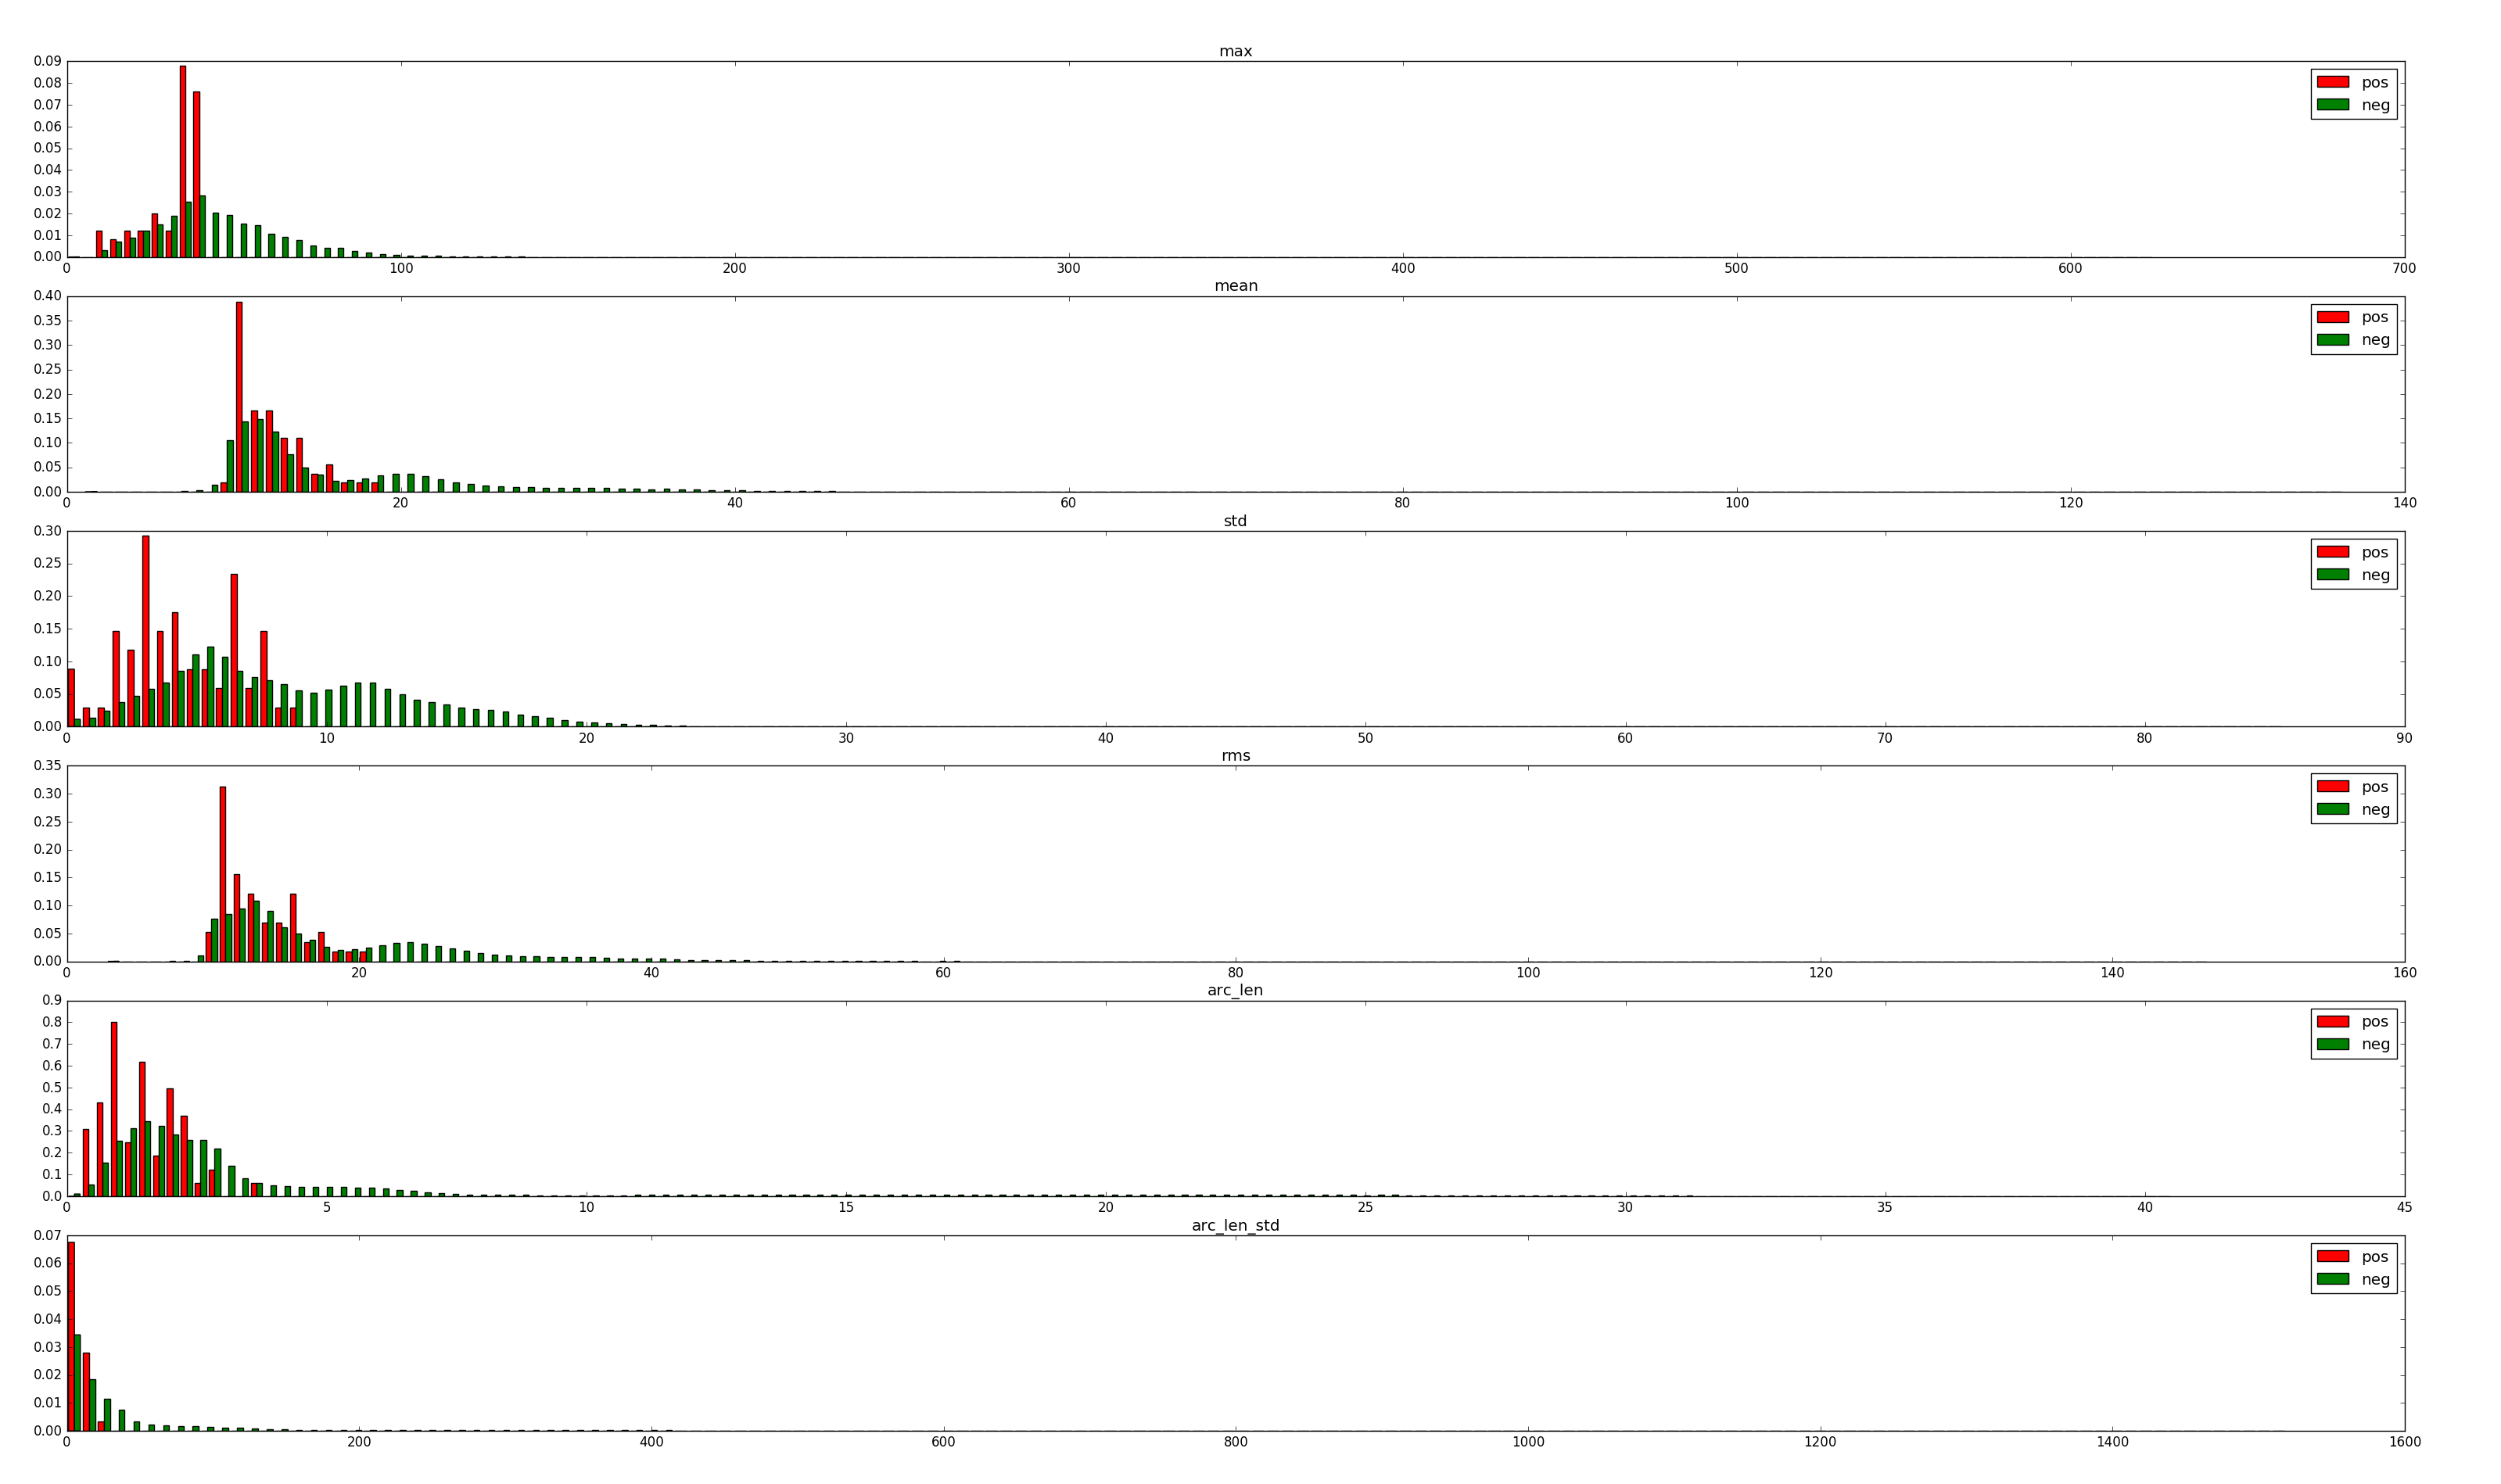
\includegraphics[width=\textwidth]{hist_features_before_win_size_1_2.png}
% \end{minipage}
% \end{center}
% \caption{Histogram for each of the 6 features for the 1-second window before the~$40 m/s^2$ spike.  The features are listed in the order presented in Section~\ref{s:features}, e.g., the top histogram is for the maximum.  Red bars indicate thefts, and green bars indicate non-theft windows.}
% \label{fig:beforehist}
% \begin{center}
% \begin{minipage}
% 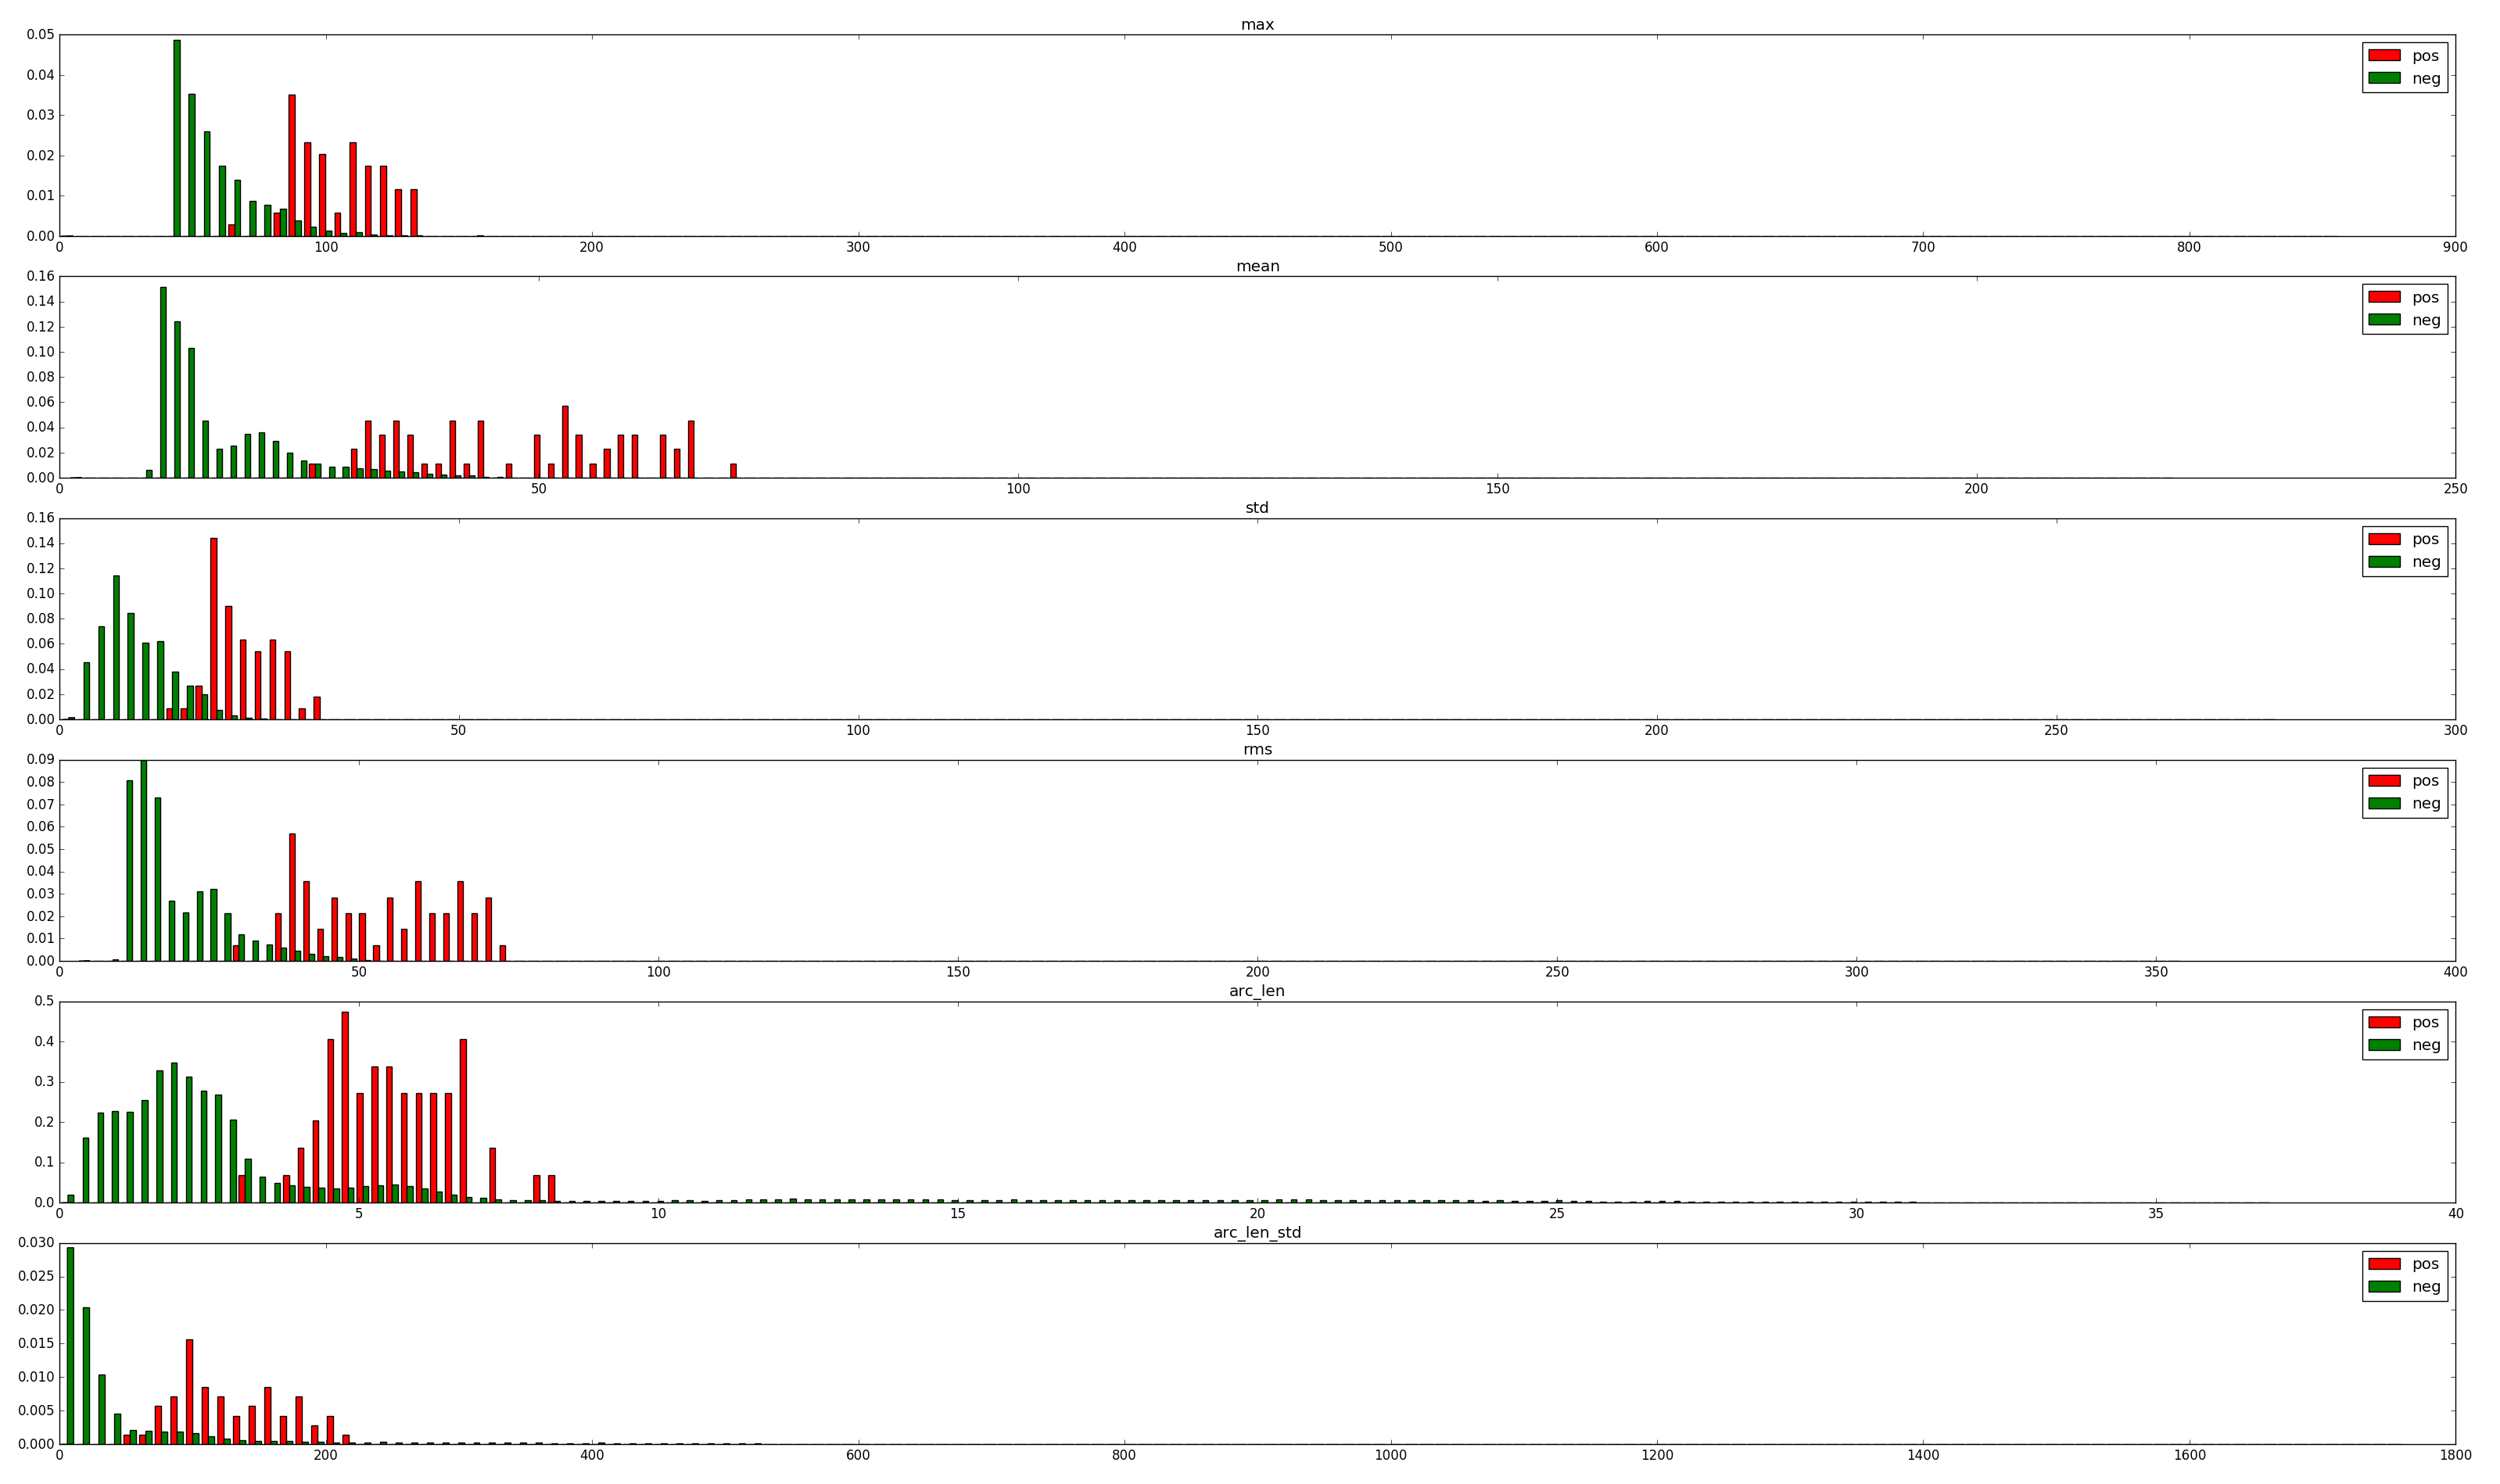
\includegraphics[width=\textwidth]{hist_features_after_win_size_1_2.png}
% \end{minipage}
% \end{center}
% \caption{Histogram of feature values in the 2-second window after the~$40 m/s^2$ spike.}
% \label{fig:afterhist}

% \end{figure*}


\begin{figure*}[t]
\centering
\begin{minipage}[t]{\columnwidth}
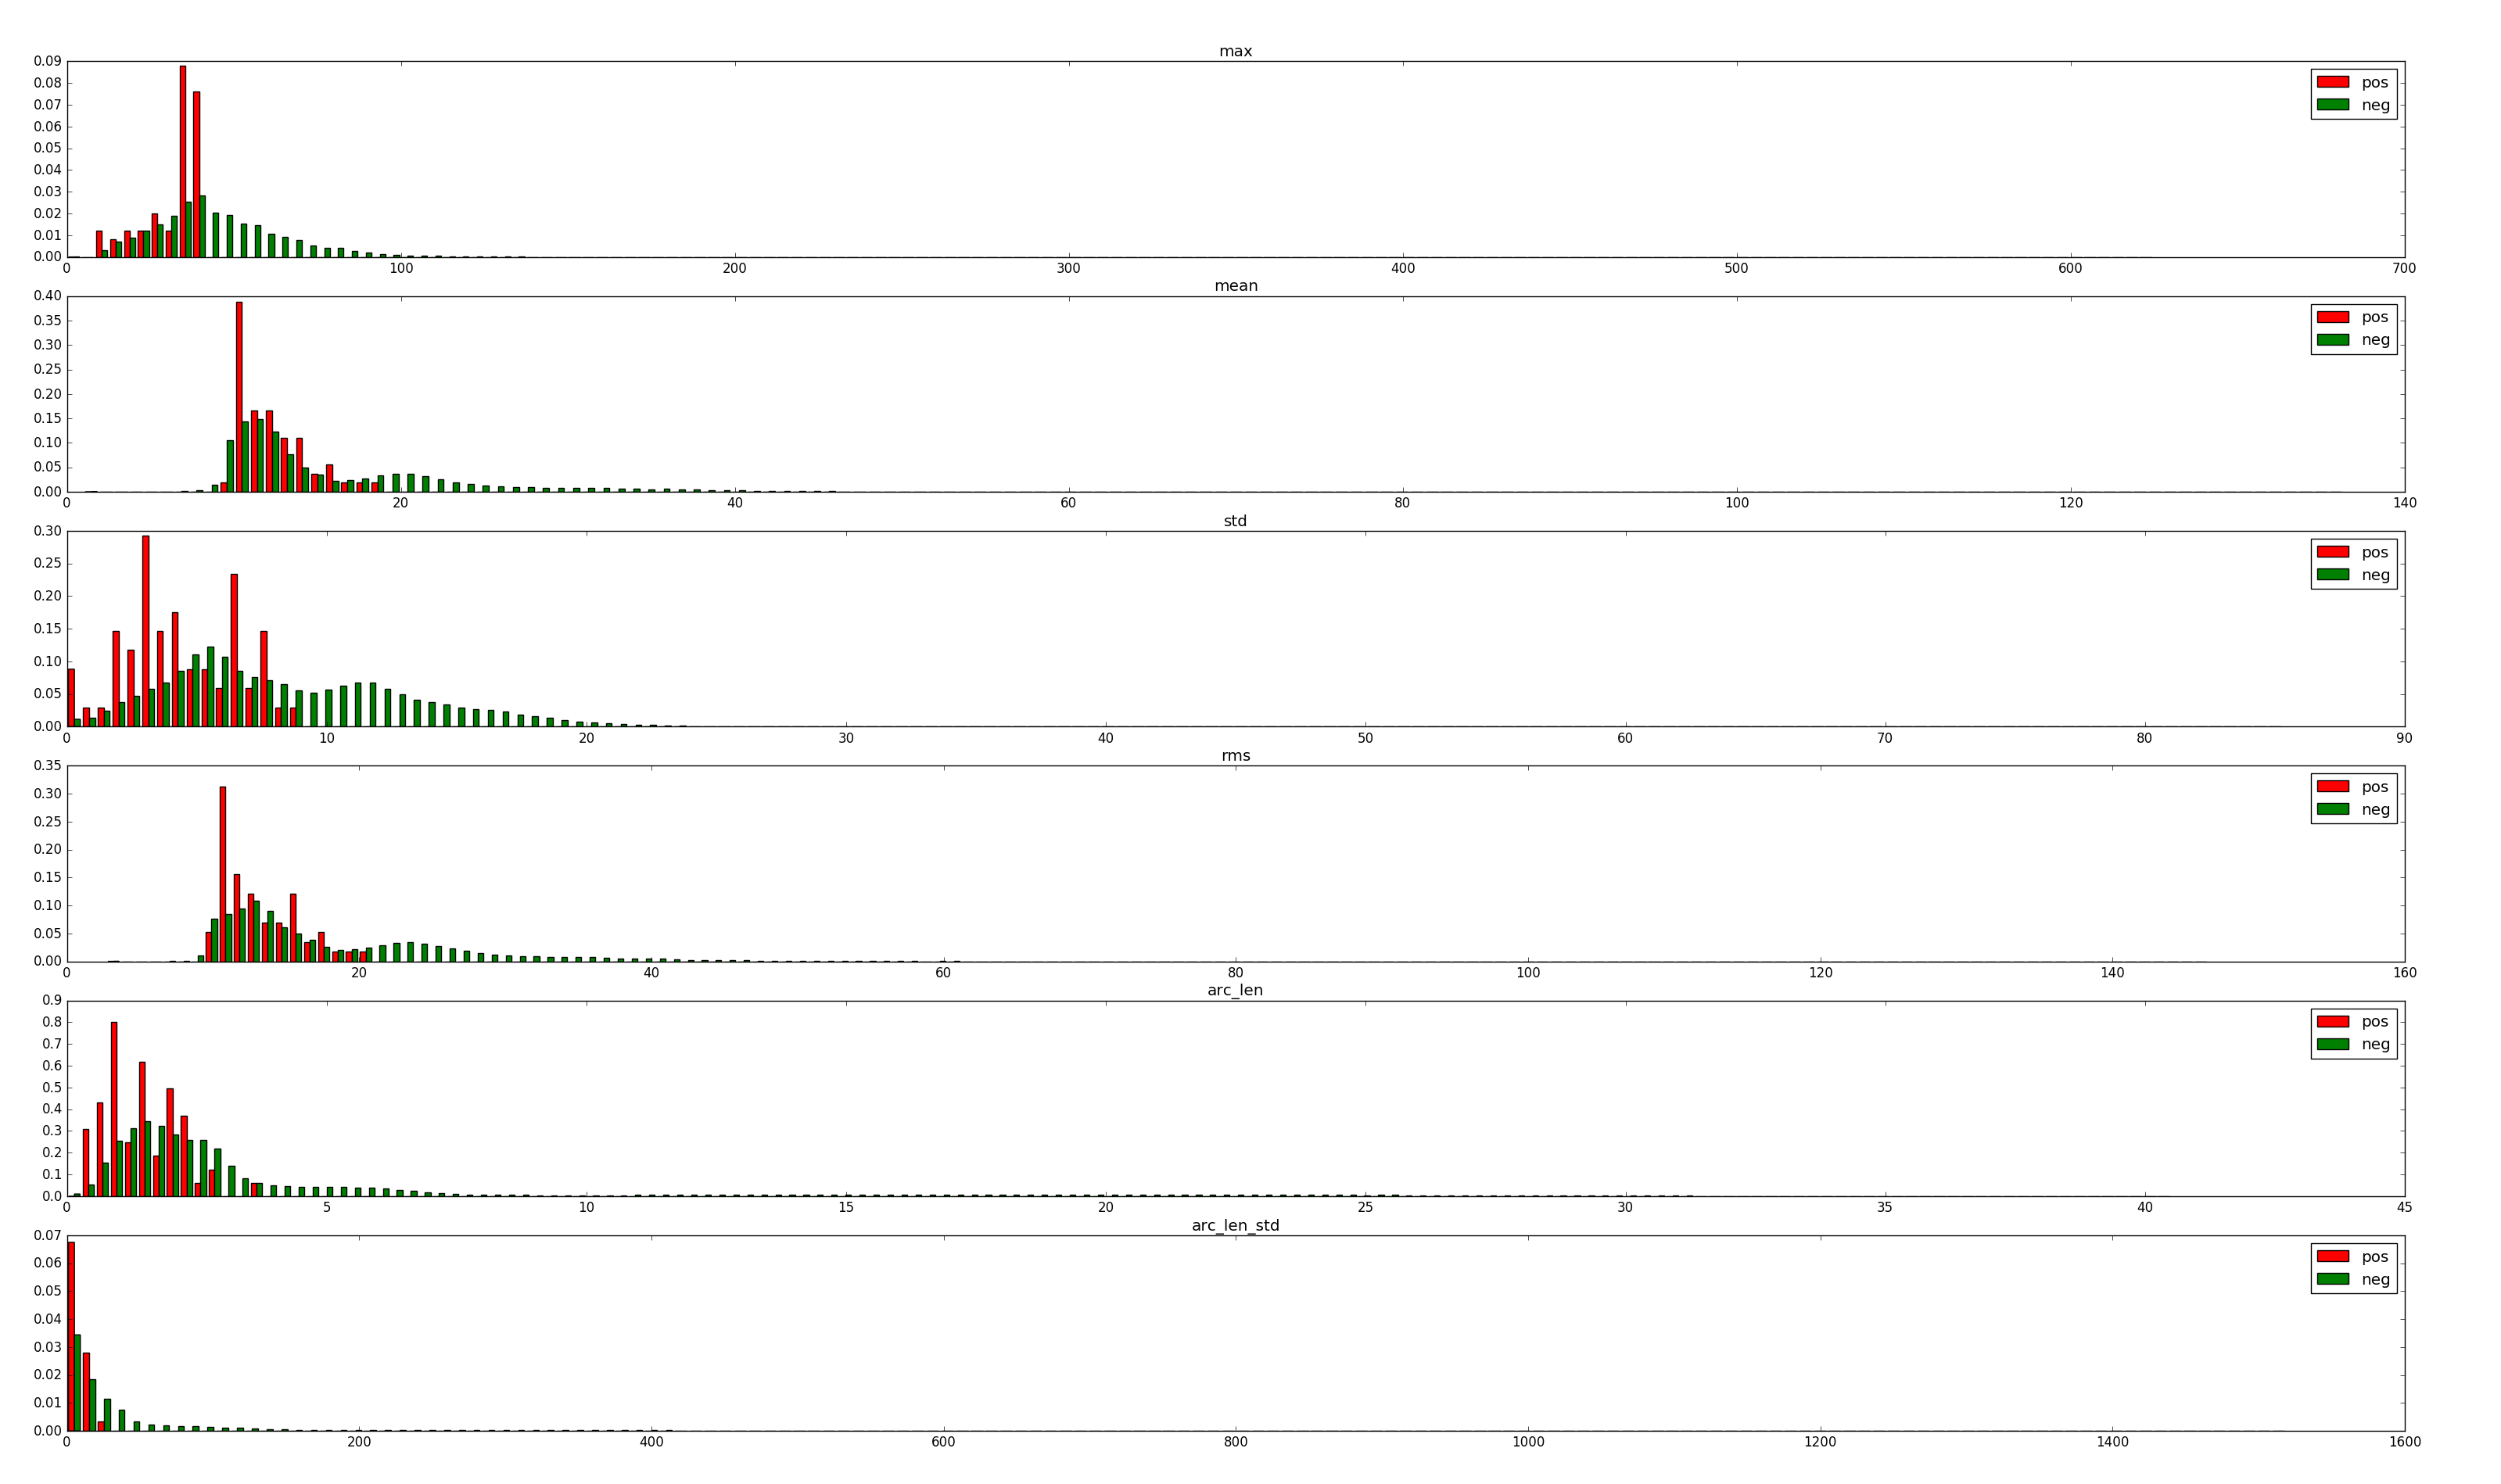
\includegraphics[width=\columnwidth]{hist_features_before_win_size_1_2.png}
\caption{Histogram for each of the 6 features for the 1-second window before the~$40 m/s^2$ spike.  The features are listed in the order presented in Section~\ref{s:features}, e.g., the top histogram is for the maximum.  Red bars indicate thefts, and green bars indicate non-theft windows.}
\label{fig:beforehist}
\end{minipage}
\hfill
\begin{minipage}[t]{\columnwidth}
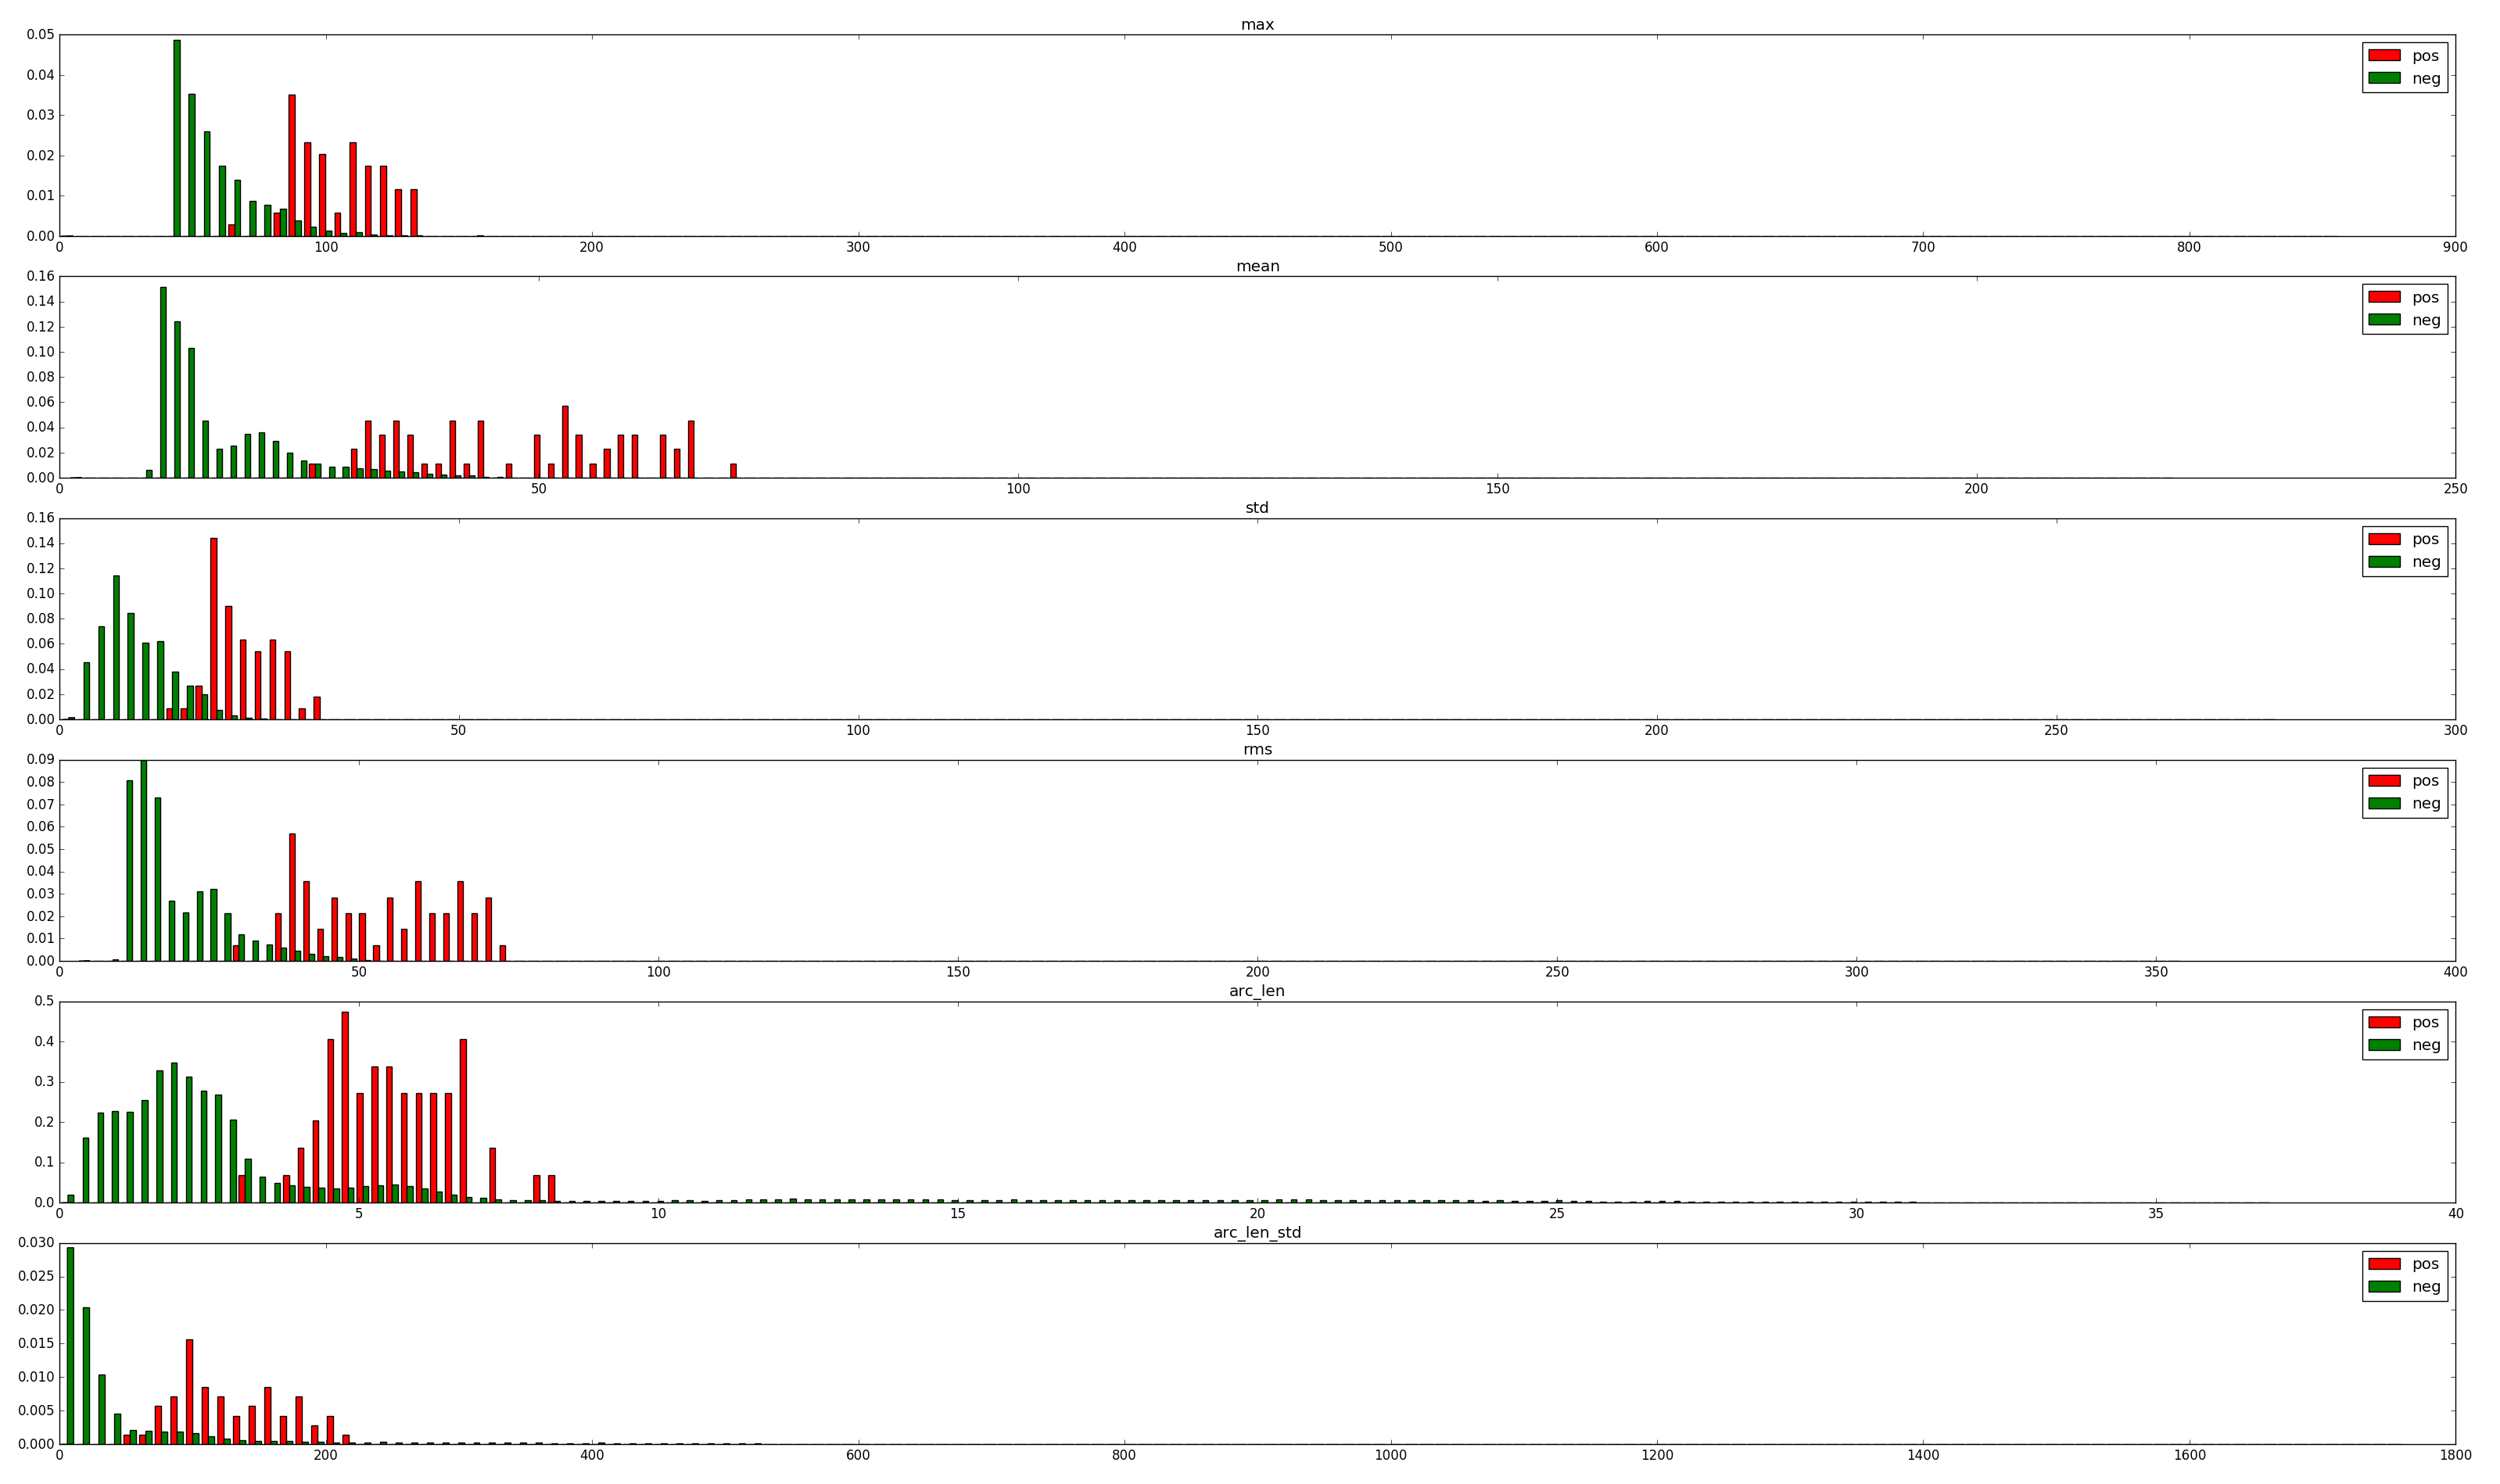
\includegraphics[width=\columnwidth]{hist_features_after_win_size_1_2.png}
\caption{Histogram of feature values in the 2-second window after the~$40 m/s^2$ spike.}
\label{fig:afterhist}
\end{minipage}
\end{figure*}

% \begin{figure*}[t]
% \begin{center}
% 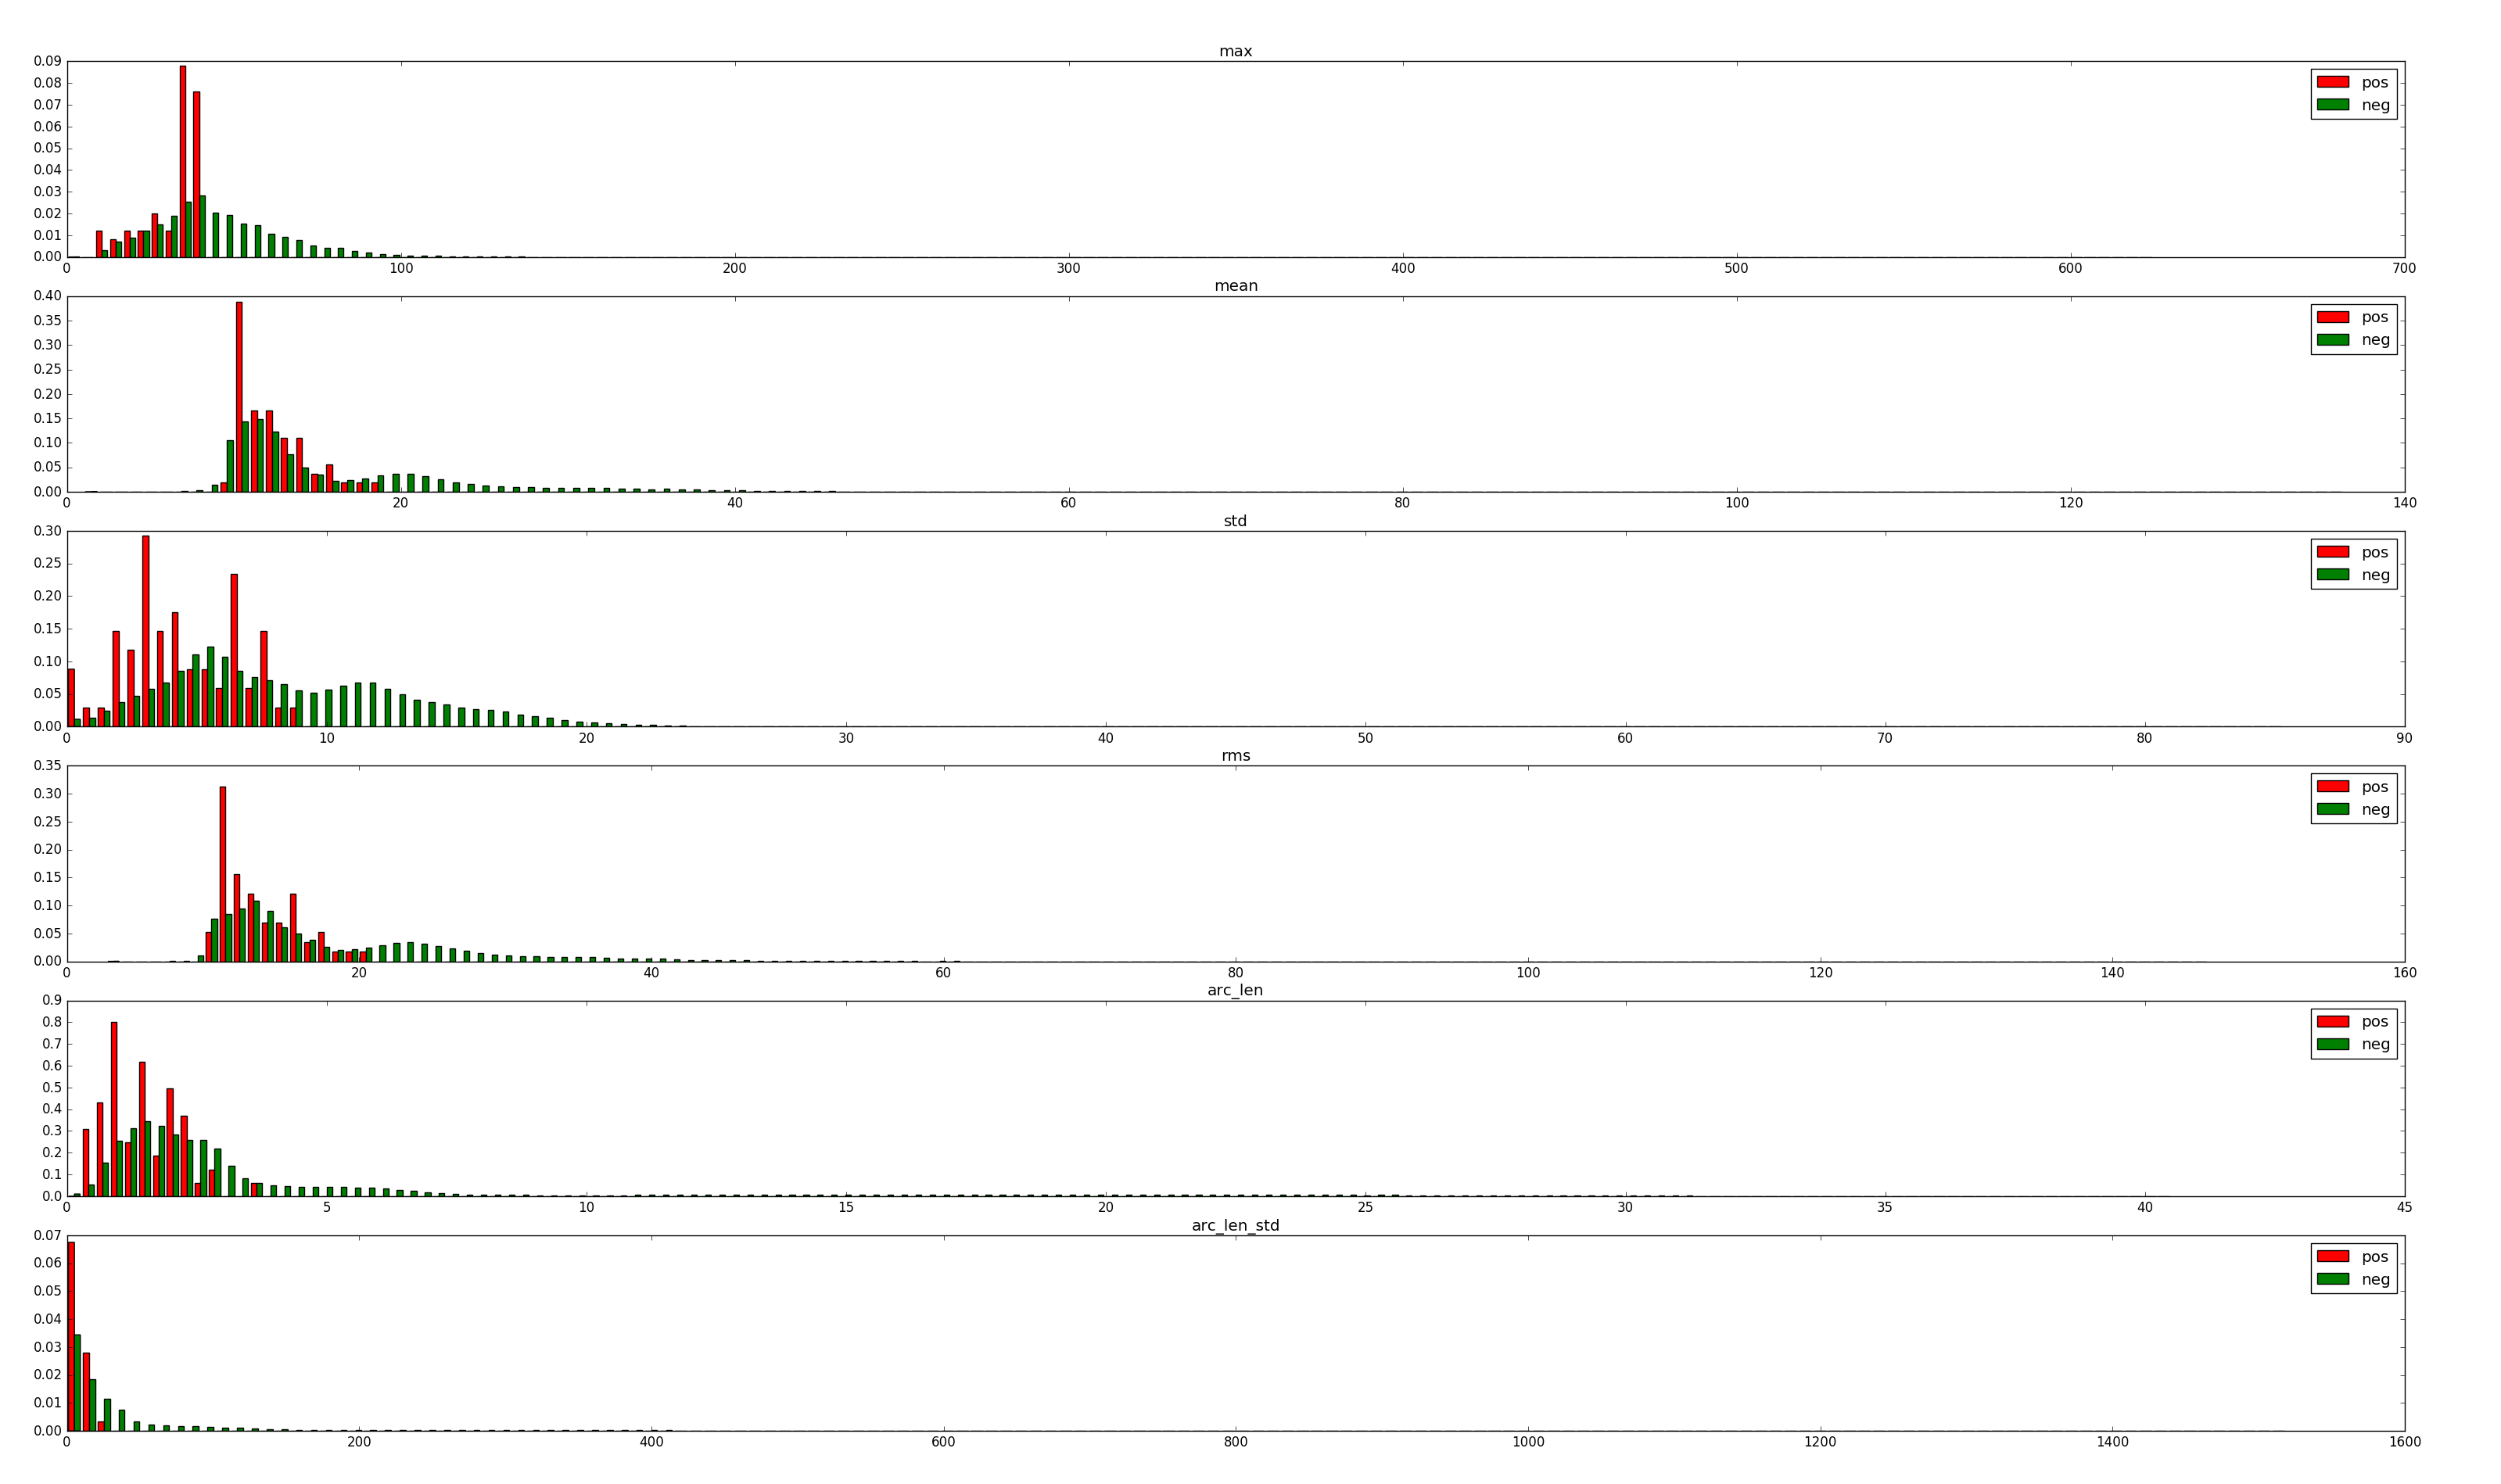
\includegraphics[width=\textwidth]{hist_features_before_win_size_1_2.png}
% \end{center}
% \caption{Histogram for each of the 6 features for the 1-second window before the~$40 m/s^2$ spike.  The features are listed in the order presented in Section~\ref{s:features}, e.g., the top histogram is for the maximum.  Red bars indicate thefts, and green bars indicate non-theft windows.}
% \label{fig:beforehist}
% \end{figure*}

% \begin{figure*}[t]
% \begin{center}
% 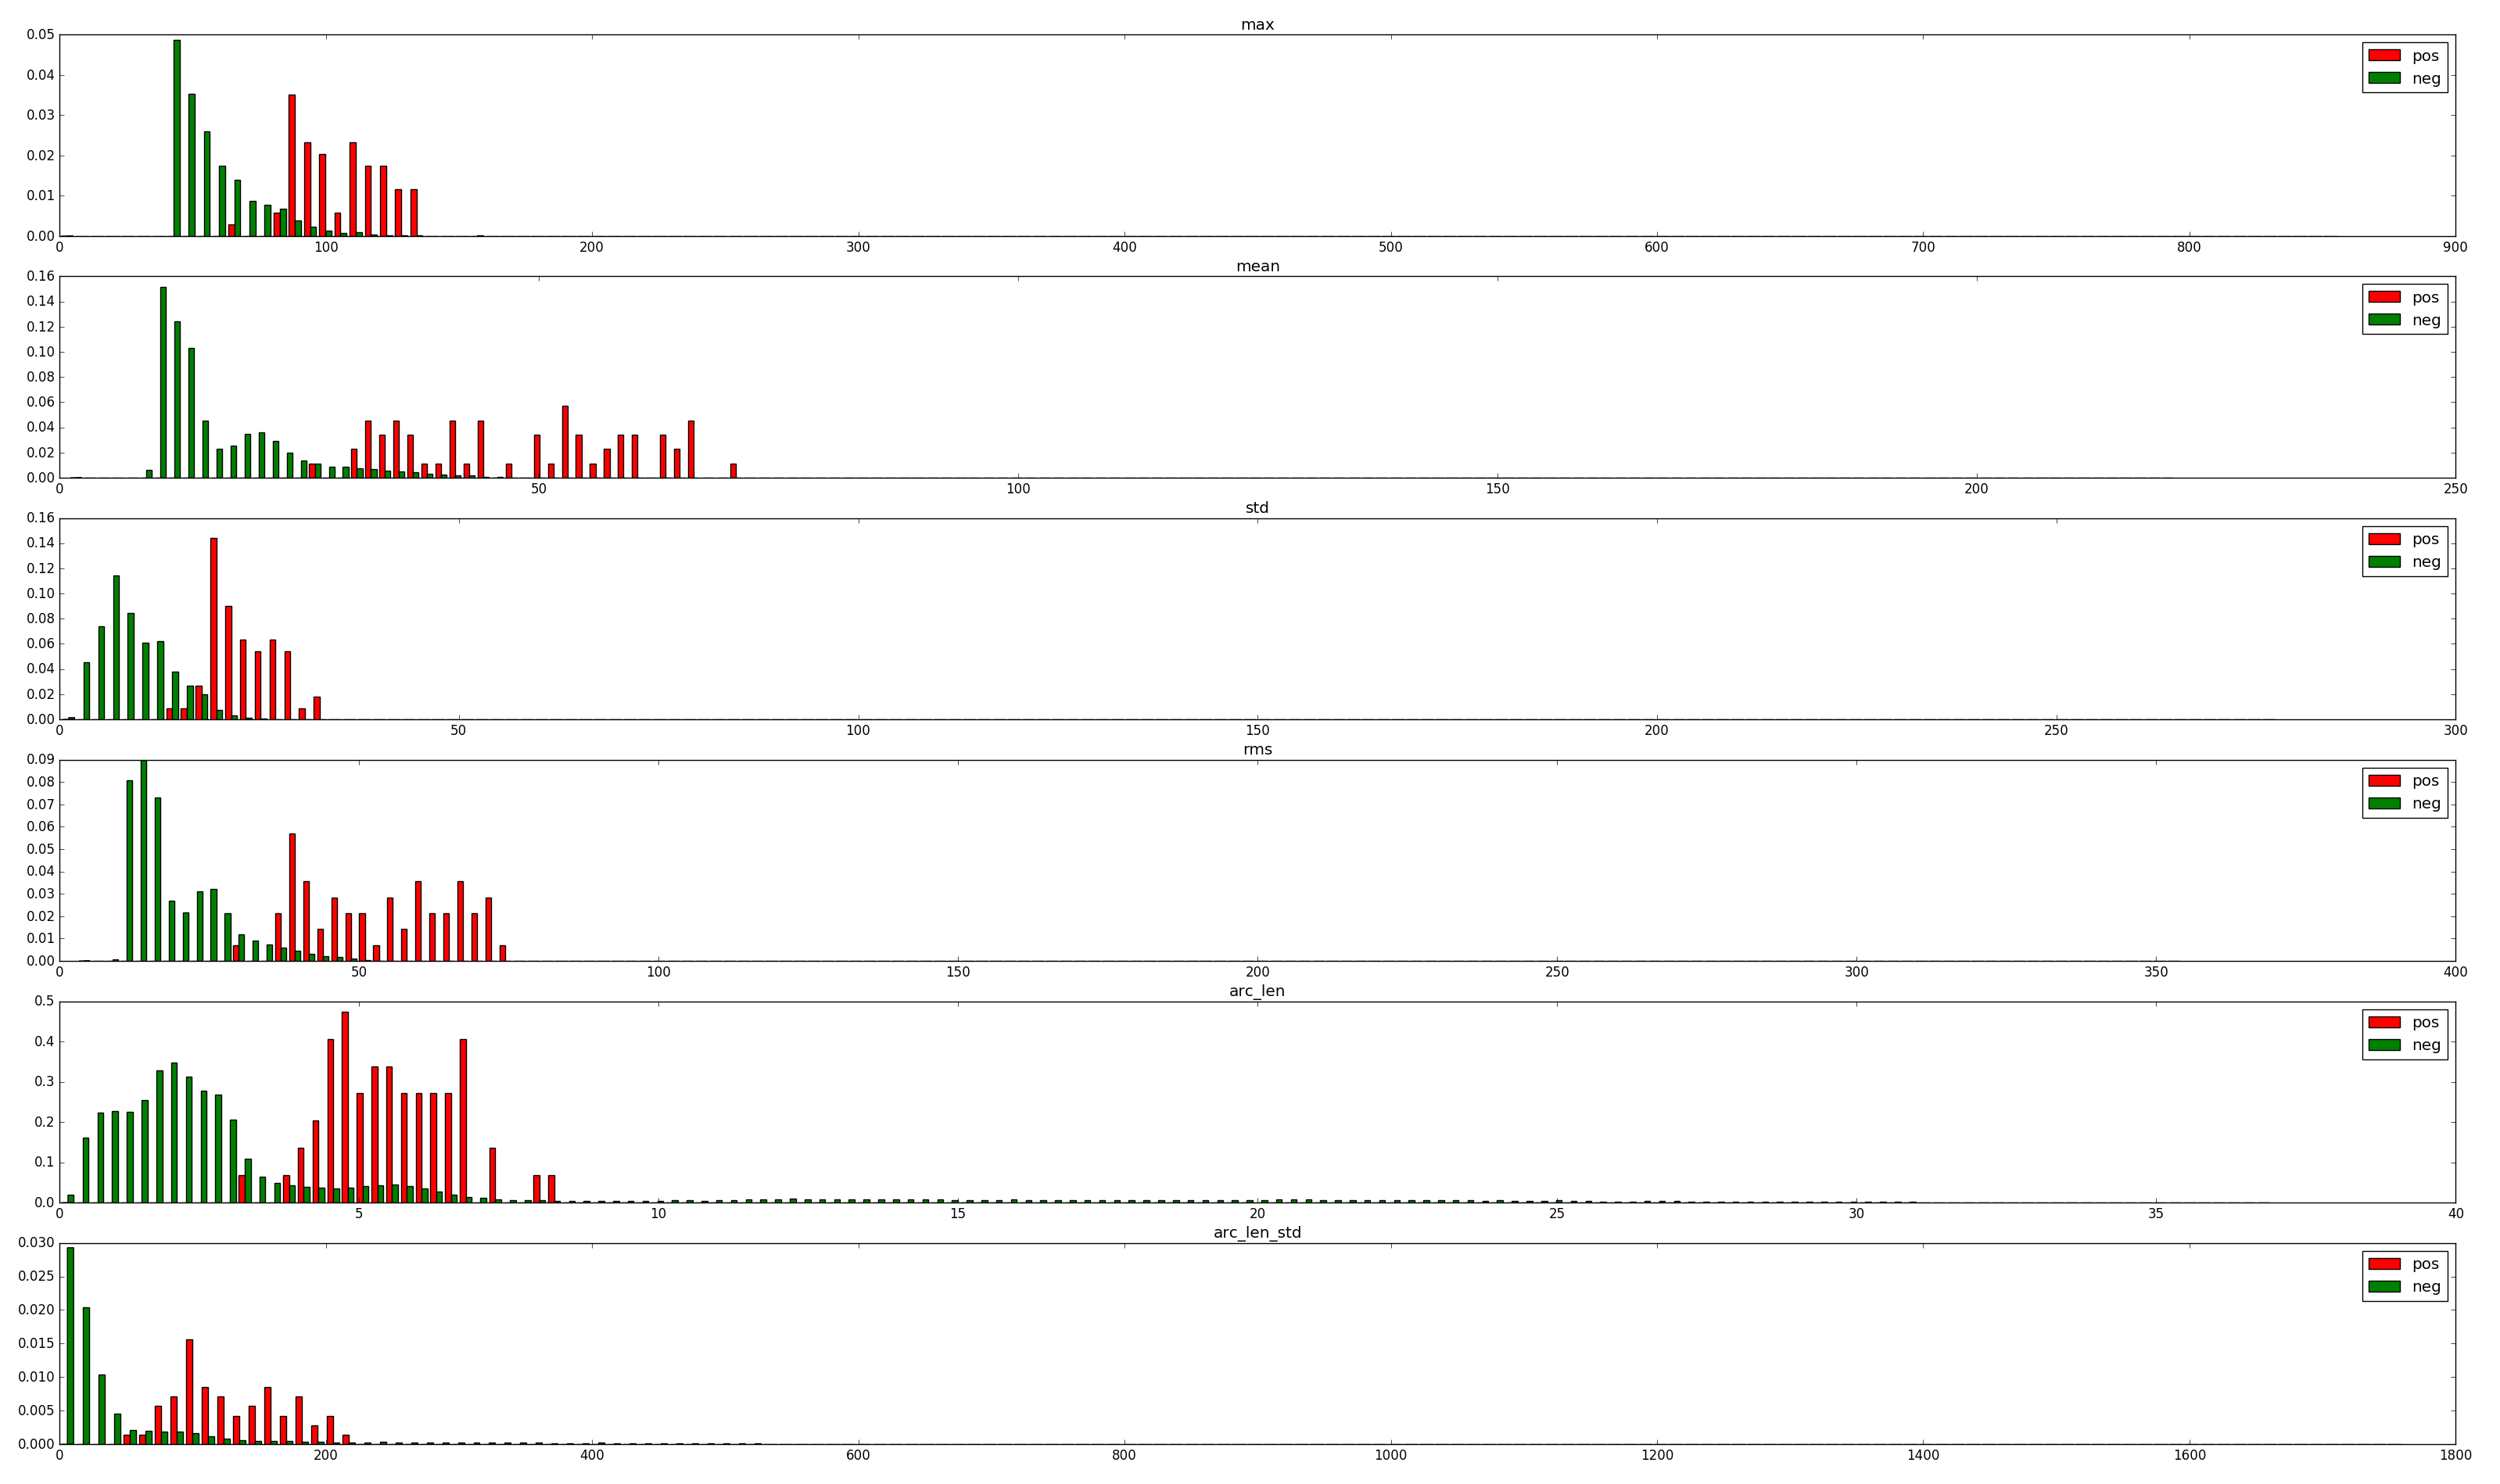
\includegraphics[width=\textwidth]{hist_features_after_win_size_1_2.png}
% \end{center}
% \caption{Histogram of feature values in the 2-second window after the~$40 m/s^2$ spike.}
% \label{fig:afterhist}
% \end{figure*}

To compare the performance of random forests and logistic regression, we fine tuned the class weights for the logistic regression classifier to lower its true positive rate until it is approximately the same as the random forests classifier, then we compared the number of false positive instances of the two classifiers.
We find that logistic regression has 14 false positive instances at a 67\% true positive rate (25 true positive instances),
while random forests has 15 false positive instances at a 62\% true positive rate (23 true positive instances).
Thus the performance of the two classifiers seems comparable in this regime.
The advantage of logistic regression is that we found adjusting class weights was more effective at controlling the false-positive/false-negative tradeoff for the logistic regression classifier.
The Receiver Operating Characteristic (ROC) curves for the logistic regression and random forests classifiers are shown in Figure~\ref{fig:roc}.

\begin{figure}[t]
\begin{center}
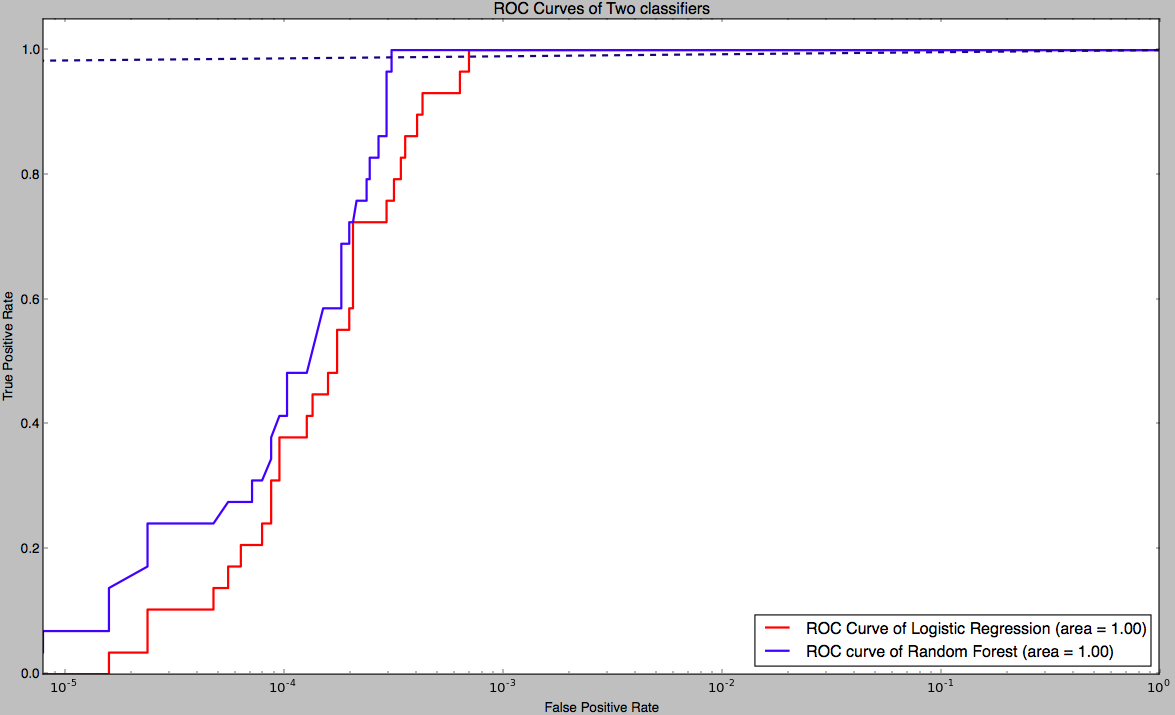
\includegraphics[width=1.0\columnwidth]{roc_curves_log_line.png}
\end{center}
\caption{ROC curves of logistic regression and random forests. The x-axis is in logarithmic scale.}
\label{fig:roc}
\end{figure}




\section{Conclusions}

In this work, we demonstrate that accelerometer data is enough to detect some common forms of smartphone theft, such as pickpocket and grab-and-run, without sacrificing user experience. 
It is remarkable that machine learning is so effective and can detect 100\% of thefts.
We suspect that this is because the kinds of theft we consider here involve a rapid jerking motion followed by the thief running away, which induces a unique pattern in the accelerometer sensor readings.

We envision that a smartphone could run our classifier continuously and automatically lock the phone whenever a suspected theft event is detected.
We expect that the inconvenience of unlocking your phone one extra time per week would be tolerable, and might not even be noticed by users.
If combined with other heuristics to reduce the false positive rate further (e.g., the phone is not unlocked within a short period after the suspected theft; the phone moves to some new location it has never been before), it might be possible to notify the owner or take other measures as well when a theft is detected.

We expect that our solution would have negligible impact on battery life and phone performance.
Modern phones support batched accelerometer sensing, where the accelerometer hardware buffers sensor readings so the application CPU only has to wake up to read sensor data when the buffer is full.
As a result, it is possible to record accelerometer sensor values at high sampling rates with negligible power draw.
Moreover, thanks to the pre-filtering (the~$40 m/s^2$ threshold),
we only need to apply the classifier on a tiny fraction of time windows (only about 10 times per hour),
so the impact on battery life should be negligible.

The primary limitation of our work is that we work with simulated thefts.
It is difficult to obtain accelerometer data on actual theft occurring in the wild, but perhaps a practical deployment could obtain such data.

It may be possible to improve our results further by using other sensors on the smartphone, such as the step counter.
The biggest open question is whether our methods can be extended to a more diverse set of theft scenarios; we hope that our work will inspire others to investigate the direction further.


% \appendix

% \section{Location}

% Note that in the new ACM style, the Appendices come before the References.

% \section{Related Work}

Many researchers have studied using smartphone sensors for continuous user authentication.
The benefit of continuous user authentication is that it happens unobtrusively, without requiring any action from users.
Continuous authentication could serve as a mitigation for theft: if the phone can detect rapidly enough that it is no longer being used by the rightful owner, it could lock itself to prevent the thief from accessing sensitive data on the phone. 

One approach is to use smartphone accelerometer data for gait recognition.
These systems often extract some features from the sensor data and then apply machine learning.
Derawi et~al.\ achieved an equal error rate of 20\%~\cite{derawi:gait}.
``Equal error rate'' is a measure of accuracy where the system is tuned so the false accept rate and false reject rates are equal, and then that error rate is reported.
Primo et~al.\ show that accelerometer-based gait authentication is somewhat dependent on the position in which the phone is held, which is a challenge for deploying gait authentication outside of a laboratory environment~\cite{primo:context}. 
They showed how to infer the position of the phone (in the person's hand vs.\ in a pocket) with 85\% accuracy, and they showed how to use this information to increase the accuracy of user authentication to 70--80\%.
They do not report performance as equal error rate.
Juefei-Xu et~al.\ show that the pace at which people walk also affects the sensor readings, and it is possible to improve accuracy by first identifying the pace at which the user is walking, then using a model tailored towards that pace~\cite{xu:pace}.
Their system achieved an equal error rate of 4--8\% (depending on the pace); or a false reject rate of 0.5--5\% at a false accept rate of 0.1\%.
Kwapisz et~al.\ generalized gait authentication to cover not just walking but also jogging and ascending and descending stairs~\cite{kwapisz:biometrics} and
achieved false reject rates of 10--15\% at a false accept rate of about 5\%.

It is not clear whether gait recognition is sufficient on its own for deployable user authentication.
One limitation is that it can only attempt to authenticate the user while the user is walking; when the user is still, it cannot infer user identity.
Another limitation is that the error rate is still fairly high: if the classifier is run continuously, once per second, even a false reject rate as low as 0.5\% will cause hundreds or thousands of false rejections per week.
Thus, gait recognition might need to be combined with other methods to yield a deployable defense against theft.

Our work builds on the methods previous researchers have used to process sensor data and extract features.
The accelerometer sensor provides raw data in the form of $X,Y,Z$ accelerations; it is useful to also compute the magnitude $M=\sqrt{X^2+Y^2+Z^2}$ of the acceleration, as that is independent of the direction of the acceleration.
Prior papers have used several methods for cleaning the raw accelerometer data, including interpolation and re-sampling to deal with irregularly sampled data and a weighted moving average filter to mitigate sensor noise.
These schemes typically divide the resulting time series into windows, each window containing about a second of sensor data.
For instance, Primo et~al.\ used overlapping windows, with each window containing 100 samples and having an overlap of 50 samples with the next window; Derawi et~al.\ and Juefei-Xu et~al.\ used non-overlapping windows, which were about 1 second in width.
Derawi et~al.\ and Juefei-Xu et~al.\ used the sensor readings as the features, while Primo et~al.\ and Kwapisz et~al.\ computed hand-crafted features from the readings, where each feature records a summary statistic on the sensor readings in the window (e.g., mean, minimum, maximum, standard deviation, number of zero crossings, etc.).

Feng et~al.\ investigated using the unique way the user picks up their phone as a biometric for user authentication~\cite{feng:pickup}. 
They achieved an equal error rate of 6--7\%.
They used the smartphone accelerometer, gyroscope, and magnetometer; in our work, we avoid the gyroscope sensor, as its power consumption is significantly higher than the accelerometer, and therefore is currently not a practical solution for continuous authentication.

Mare et~al.\ developed a continuous authentication system where the user wears a smartwatch or bracelet, which is used to authenticate the user to their computer~\cite{mare:zebra}. 
Their continuous authentication scheme works well and could plausibly be used to authenticate to a smartphone, but it requires users to wear a bracelet; in contrast, we seek solutions that do not require the user to carry or wear any additional devices.

The most closely related work is by Chang et~al.\, who used the way
that each person takes their phone out of their bag or pocket as a 
form of biometric authentication~\cite{cheng:theft}.
They use accelerometer and gyroscope data to detect when the user picks
up their phone, and then they apply dynamic time warping and boosting to
determine whether the pickup motion matches known templates from the
owner of the phone.
Their system achieves a 10\% false positive rate and a 5.5\% false negative rate, which are relatively high,
considering that users may pick up their phones dozens of times each day.

The prior work focuses on authenticating the user.
In contrast, we take a different approach: we attempt to detect the
specific motion pattern that occurs during a grab-and-run or pickpocket theft.
The benefit of biometric authentication is that it provides a comprehensive
way to detect theft, regardless of the way the phone was stolen; however,
as summarized above, the false positive rates of existing schemes
are fairly high.
Our scheme is limited to detecting a particular type of theft, but achieves
far lower false positive rates.
Our classifier is also user-independent and does not require obtaining
training data from each user; we use the same classifier for all users.




\section{Methodology}

In this section, we describe the data collection software, which we used to gather positive and negative data for our training and test sets as well as the feature extraction scheme, and other classifier design decisions.

\subsection{Data Collection}

\subsubsection{Software}
We used an Android application to record data from the smartphone's 3-axis accelerometer, which then encrypted it and stored it in the cloud.
We acquired sensor data at the highest sampling rate supported by the phone using SENSOR\_DELAY\_\\FASTEST~\cite{android:doc}. 
On most devices, including the one we used for the simulated theft experiment, the sampling rate is 100 Hz. 

\subsubsection{Simulated Theft Experiment}
Because data from real thefts is hard to obtain, we simulated three types of common smartphone theft scenarios, based on campus police alerts that we receive, with one researcher acting as a smartphone user and another one playing the role of a thief. 
The three theft scenarios are as follows:
\begin{enumerate}
\item The user stands still and holds the phone with one hand as she is using the device, for instance reading a text; the thief approaches from behind, grabs the phone with both hands and runs away in the forward direction. 
\item The user holds the phone in front of her with one hand while walking at a constant speed; the thief approaches from behind, grabs the phone with both hands and runs away in the forward direction. 
\item The third scenario simulates pick-pocket thefts. The user places the phone in the back pocket of their pants and stands still; the thief approaches from behind, steals the phone from user's pocket and runs away in the forward direction.
\end{enumerate}
We collect 40 instances of each scenario, for a total of 120 trials. 
Data collection was split across four sessions, each consisting of 10 trials per scenario, with different researchers acting as the victim and thief in these two sessions. 
We ran the experiment on flat ground in an open space, so the experiment was not interrupted. 
We also made sure that the thief ran at least 40 feet after gaining possession of the victim's phone.
We used a Nexus 5X smartphone (InvenSense MPU6515 embedded accelerometer) with Android version 7.1.1 for data collection in our simulated theft experiment.
Figure~\ref{fig:simtheft} plots one example of accelerometer readings from a single simulated theft.


\begin{figure}[t]
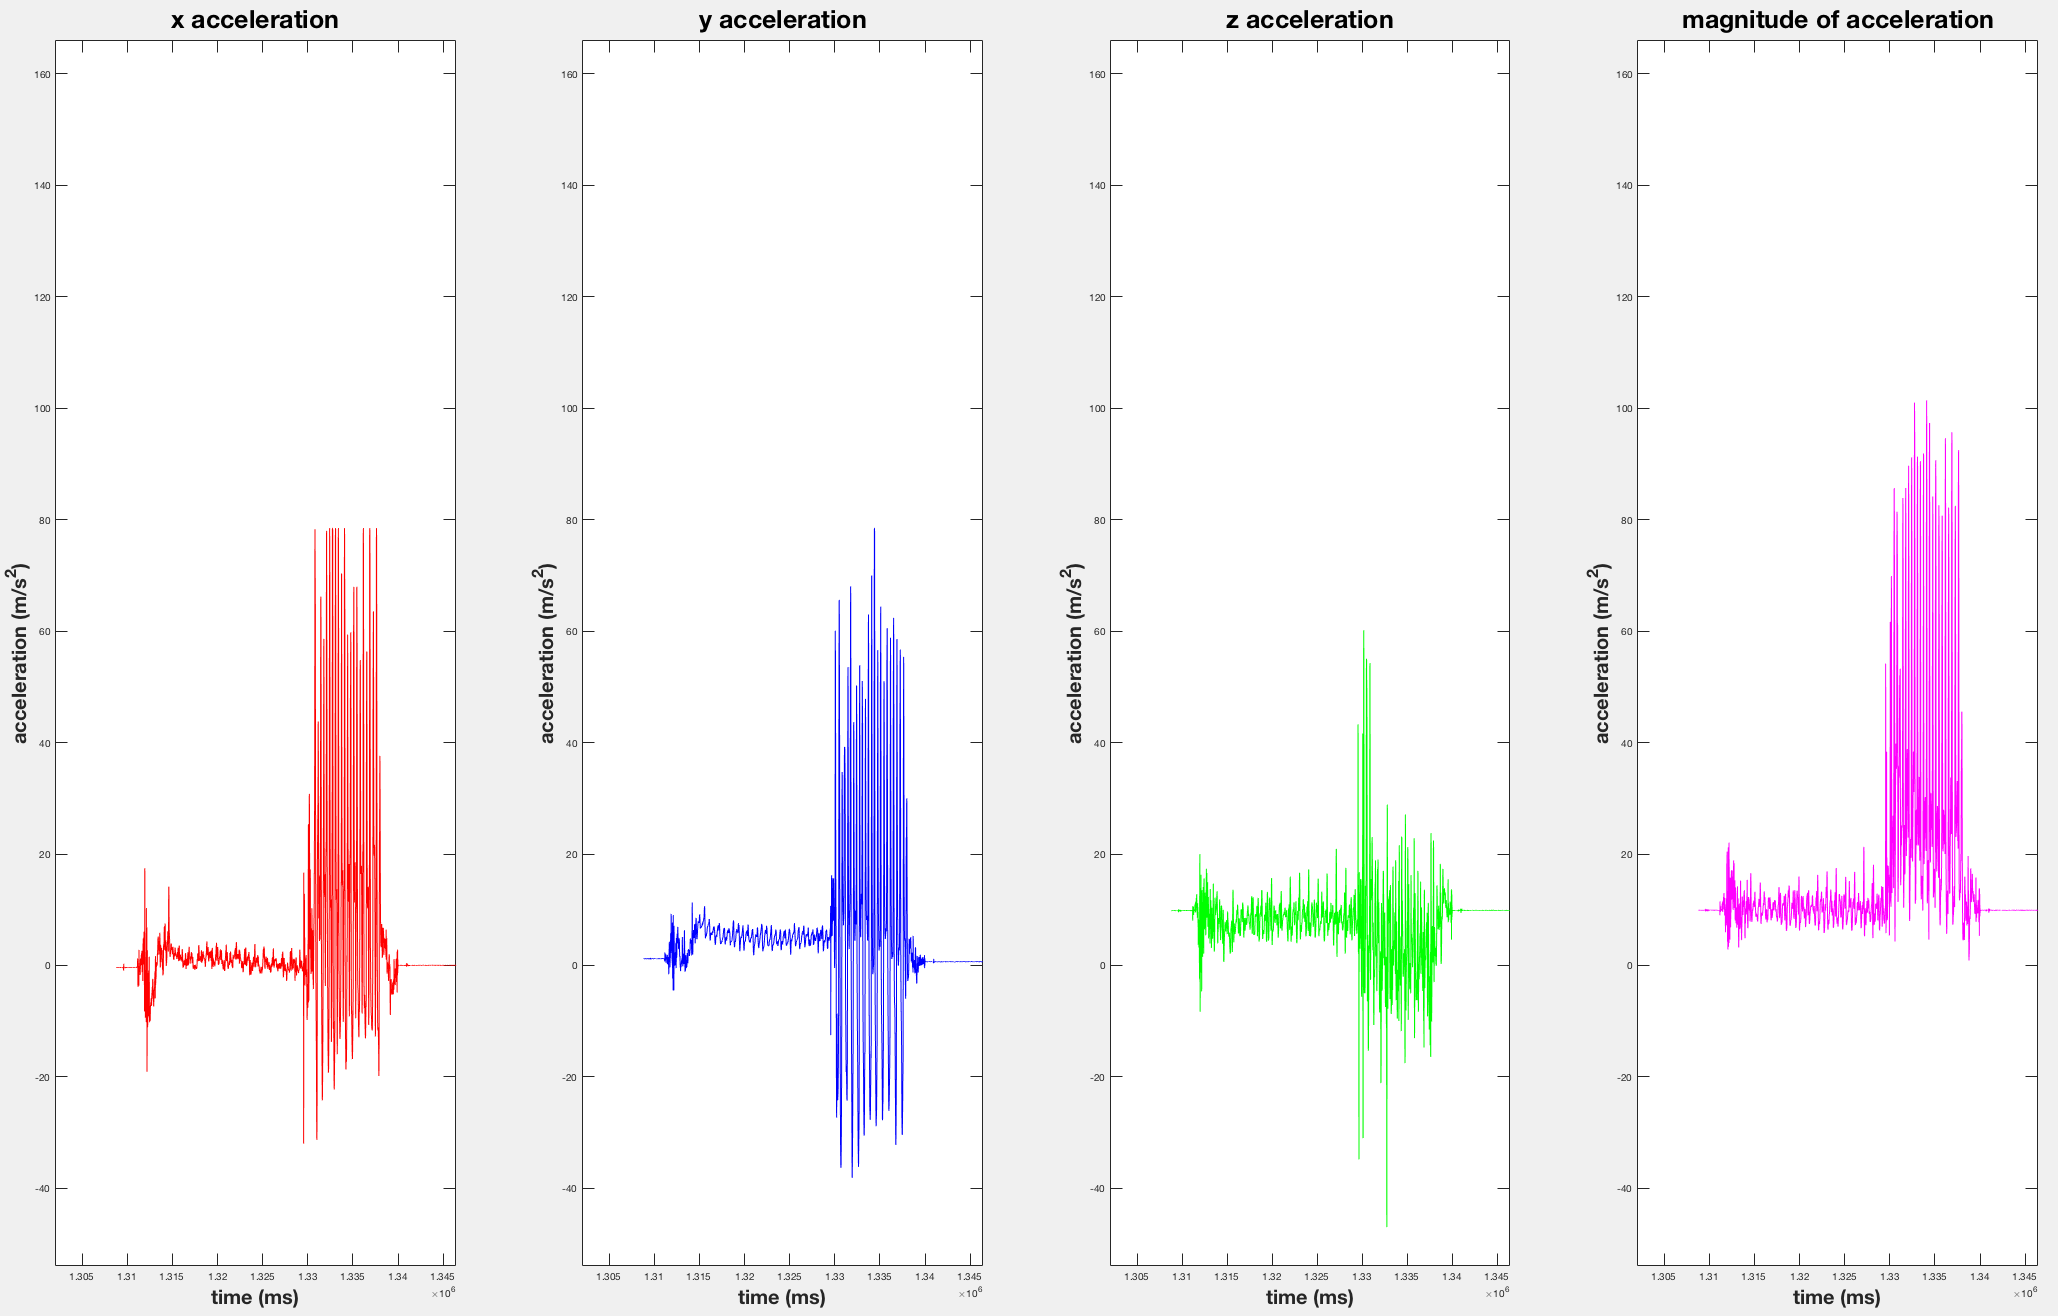
\includegraphics[width=1.0\columnwidth]{pos_acc_separated.png}
\caption{The X, Y, Z and magnitude of acceleration, respectively, from one simulated theft instance.}
\label{fig:simtheft}
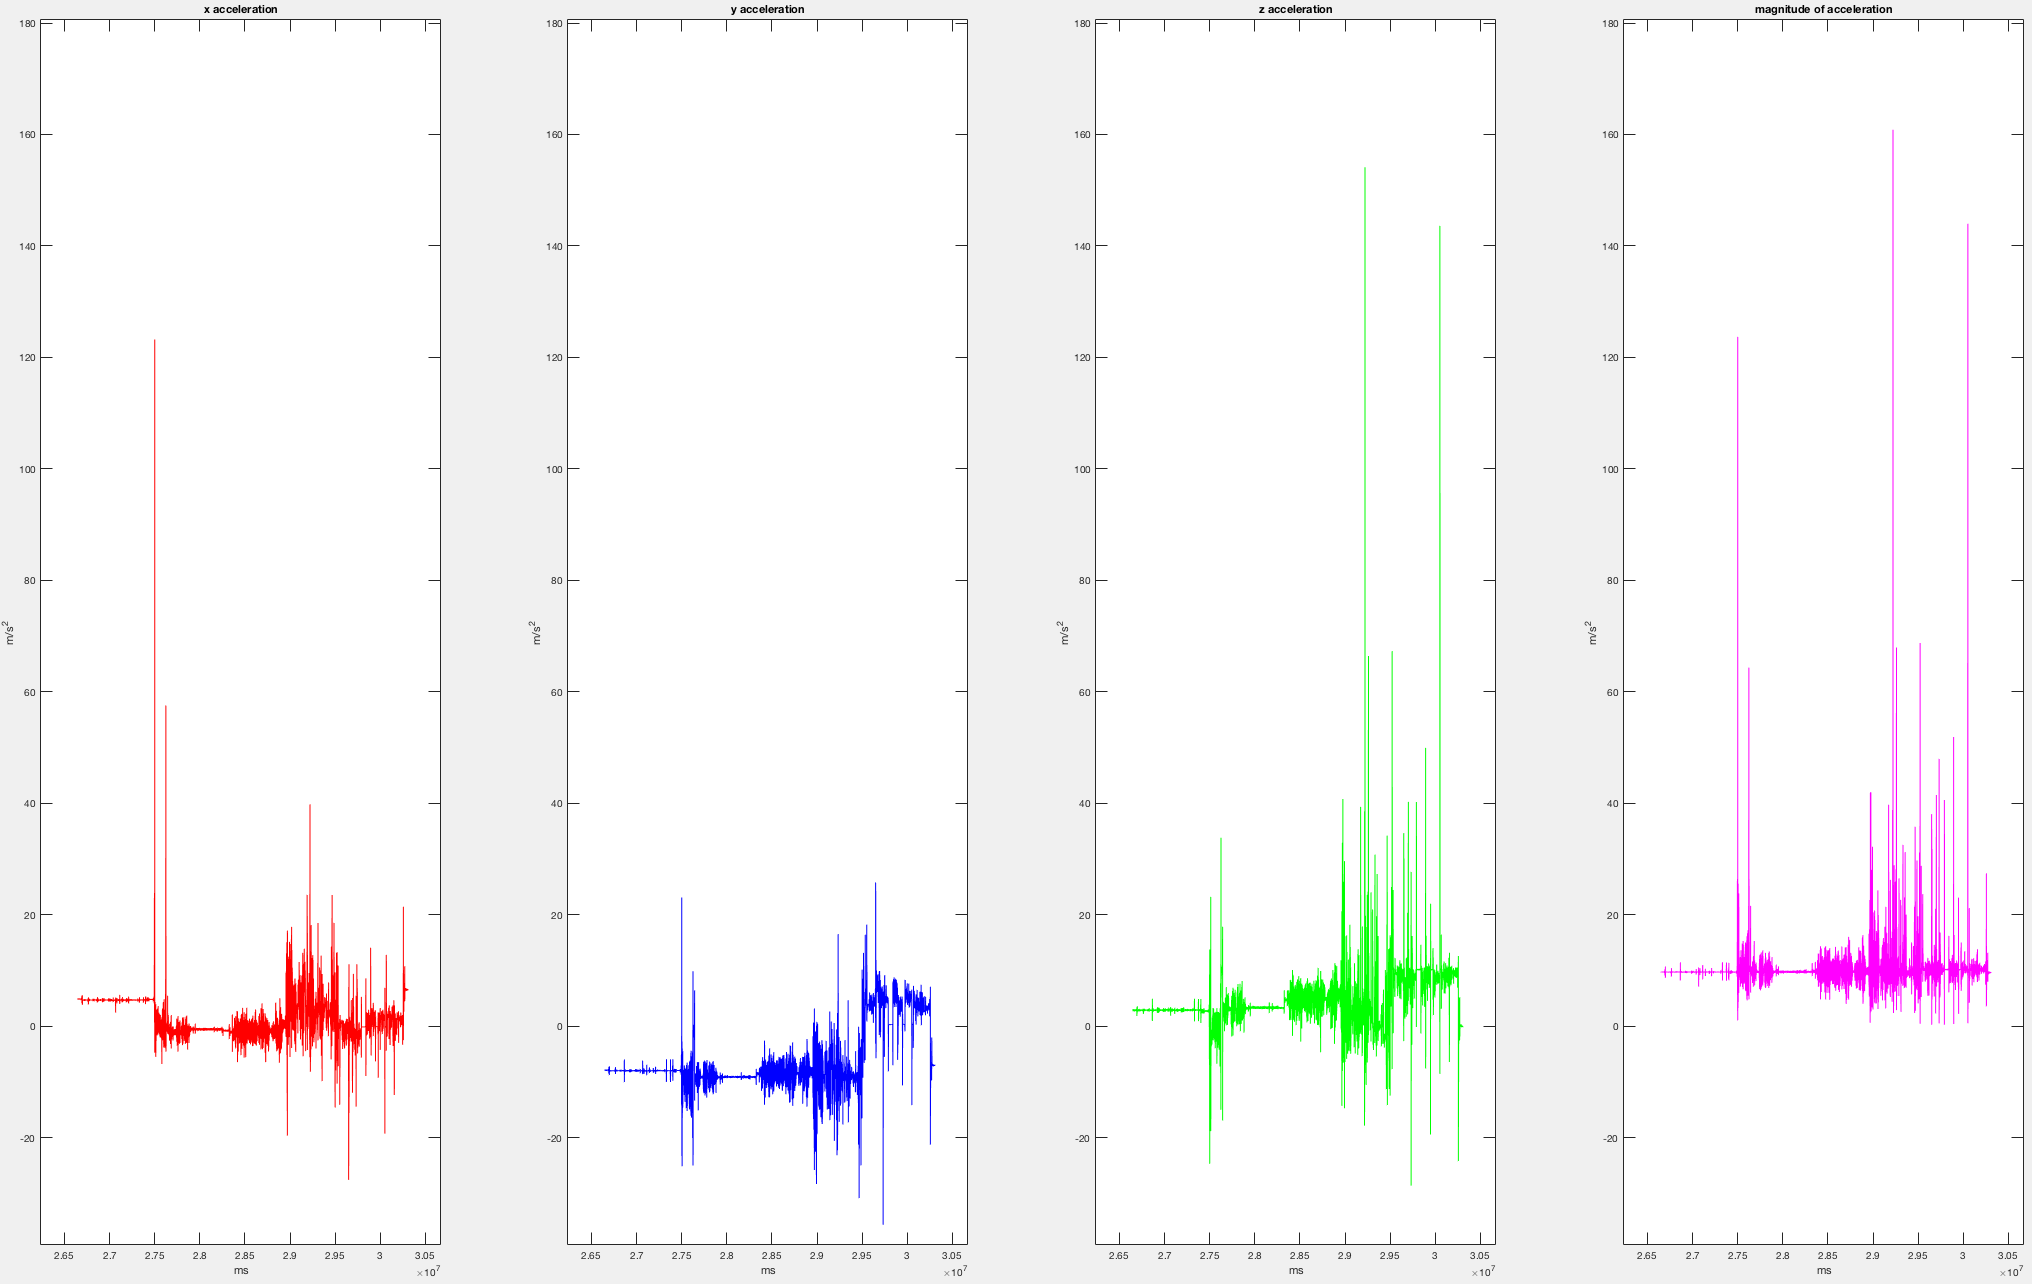
\includegraphics[width=1.0\columnwidth]{neg_acc_separated.png}
\caption{The X, Y, Z and magnitude of acceleration, respectively, during normal usage at an arbitrary time period.}
\end{figure}




\subsubsection{Field Study}
We performed a field study to gather data from ordinary smartphone users while they perform everyday activities, including walking, running, driving, possibly excercising, and anything else that occurred during their lives over the field study period.
% We obtained approval from the University of California, Berkeley IRB (Institutional Review Board) for this study. 
We obtained approval from our university IRB for this study. 
The study was conducted in a metropolitan area from September to December 2016.
% The study was conducted in the Bay Area of the United States from September to December 2016.
None of the participants experienced a phone theft during the study interval,
so we were able to use the accelerometer data collected from the user study as negative samples for our machine learning algorithms (i.e., instances of non-theft activity).

We posted a recruitment advertisement on Craigslist in September 2016. 
% We posted a recruitment advertisement on the Craigslist under the SF Bay Area `jobs et cetera' category in September 2016. 
We only recruited participants who used an Android smartphone with version 5.0 and above. 
After obtaining their consent, we installed our data collection application on their phones and collected data for a three-week period.
The application ran in the background and collected accelerometer sensor readings continuously, 24 hours a day.
We contacted participants weekly to make sure their phones were functioning correctly and troubleshoot any data collection issues.
Each participant was paid \$150 for their participation.

The study was divided across 3 rounds; each round lasted 3 consecutive weeks. 
A total of 55 participants were recruited, and
53 out of the 55 subjects completed the study. 
In the first round, 2 of the 18 participants did not complete the study.
Detailed demographic information about the participants of this user study is listed in Table~\ref{tbl:demographics}.
In aggregate, they used 21 different smartphone models from 6 different manufacturers and 8 different Adroid versions. This ensures the dataset containing diverse devices, and the classifiers are not specific to a particular type of smartphone or Adroid version.
We also asked participants how they typically carried their phone, when it was not in their hands; 33 reported keeping it in their pockets, 9 in their purses, 12 in multiple locations (e.g., pocket or purse, pocket or backpack), and 1 did not respond.
During the study, the subjects carried their phones while performing daily activities, for example walking, driving, running and possibly excercising. Data from a wide variety of real-world activities ensures the generability of the classifiers trained on it. 

\begin{table}[H]
\centering
\begin{tabular}{rrrrrr}
\hline
      & Male & Female & Age 20--29 & 30--39 & 40+ \\ \hline
R1    & 5    & 11     & 8         & 6     & 2   \\
R2    & 10   & 8      & 7         & 7     & 4   \\
R3    & 11   & 8      & 9         & 4     & 6   \\
Total & 26   & 27     & 24        & 17    & 12  \\ \hline
\end{tabular}
\caption{Participants' demographic information.}
\label{tbl:demographics}
\end{table}




\subsection{Feature Extraction}
\label{s:features}

Our theft scenarios all involved a sudden movement of the phone, which causes a large acceleration.
Therefore, as a first filtering step, we filtered the data to focus on times near when a large motion occurs.
In particular, our classifier is activated when the magnitude of acceleration $M$ exceeds~$40 m/s^2$.
We extract a one-second window before the activation time and a $n$-second window after the activation time, compute features on each of these windows, and use them for classification.
We vary $n$ from 1 to 7 to obtain the best classification accuracy.
We chose a threshold of~$40 m/s^2$ as all of our simulated thefts experienced accelerations exceeding that threshold when the phone was initially grabbed by the thief.

We first identified 16 candidate features, 8 features for each of the two windows.
In particular, we computed the minimum, maximum, mean, standard deviation, root mean square, arc length, product of arc length and standard deviation, and mean absolute value, each computed on the magnitude values ($M$) within the window.
We chose to only compute these features on the magnitude of the acceleration, and not the $X$, $Y$, and $Z$ components, because the magnitude is non-directional and thus more robust to changes in the orientation of the phone. 
We then visualized the distribution of these features for the two classes and applied feature selection techniques to choose a subset of features that yield good performance.
We removed the minimum and mean absolute value from the feature list because removing them did not affect the performance of the classifiers. 
As a result, we extract a 12-dimensional feature vector, 6 features from the before-window and 6 from the after-window, every time the detector is triggered.

Let $M_1,\dots,M_k$ denote the time series of acceleration magnitudes within the window.
The features are computed as follows:
\begin{itemize}
\item \emph{Maximum}: the maximum value of the magnitude within the window, i.e., $\max(M_1,\dots,M_k)$.
\item \emph{Mean}: the average value of magnitude in a window, i.e., $(M_1+\dots + M_k)/k$.
\item \emph{Standard deviation}: the standard deviation of magnitude values in a window.
\item \emph{Root mean square}: the RMS of magnitude values in a window, i.e., $(M_1^2 + \dots + M_k^2)^{1/2}/k^{1/2}$.
\item \emph{Arc length}: the average of the absolute differences between all adjacent magnitude values in a window, i.e., $(|M_2-M_1| + |M_3-M_2| + \dots + |M_k-M_{k-1}|)/(k-1)$.
Intuitively, this captures the average of the first derivative of the acceleration.
\item \emph{Product of arc length and standard deviation}: the product of the two feature values.
\end{itemize}

Because the accelerometer sensor reports readings in the same units on all Android phones, and because our features are relatively simple, we believe these features capture fundamental, device-independent characteristics of the motion rather than anything specific to the particular device used for data capture (e.g., in contrast to the hardware-based differences documented by Dey et al.~\cite{Dey2014}).

We obtained 60 positive instances from the 60 simulated thefts.
After applying the~$40 m/s^2$ threshold, we obtained approximately approximately 248,000 negative samples from the data collected in the field study. 
We then applied boolean classification techniques to this data set.


% \begin{figure}[t]
% 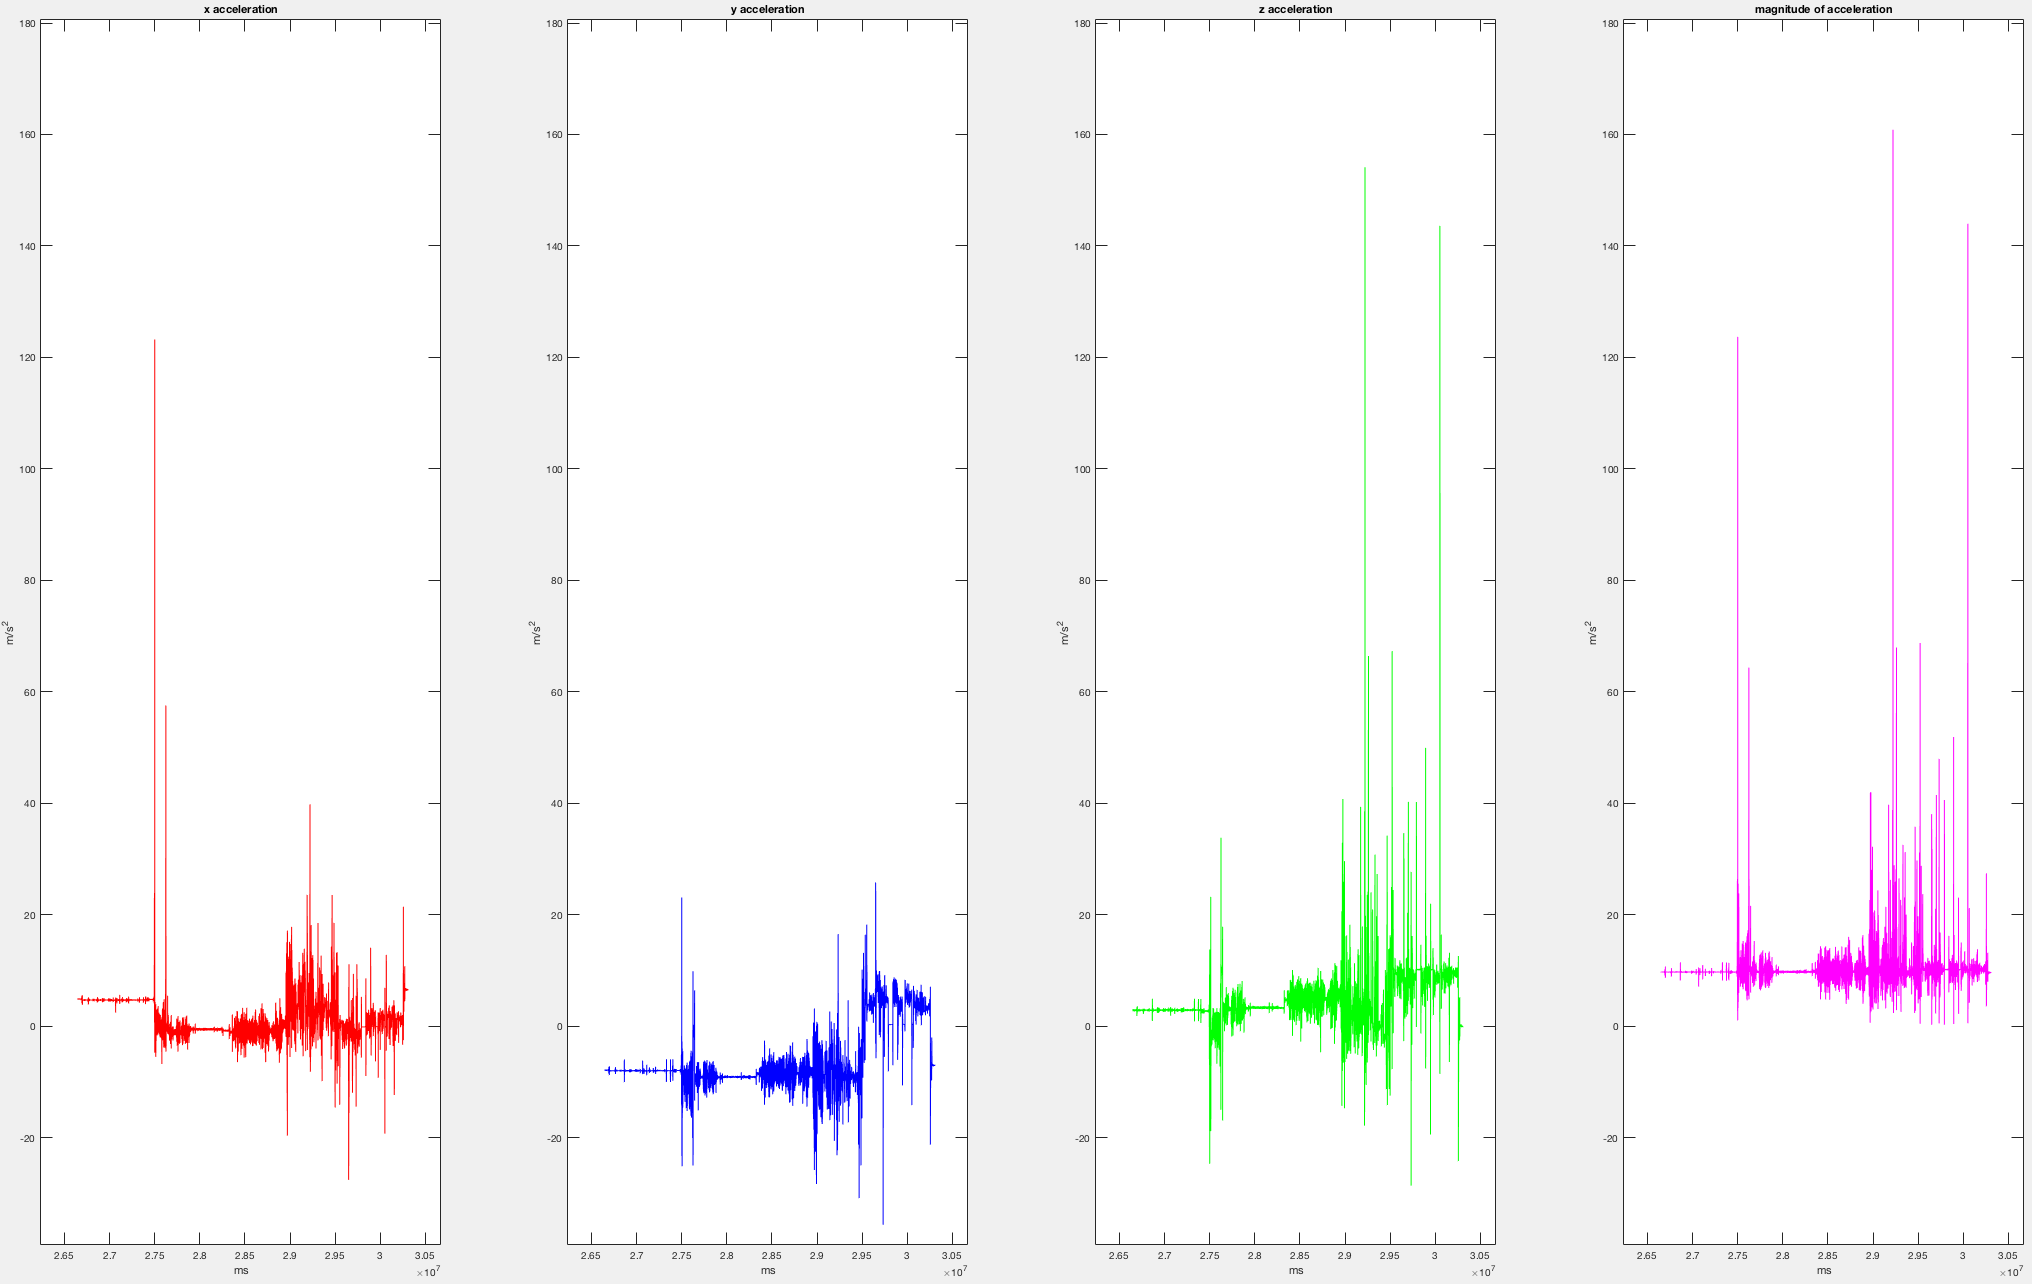
\includegraphics[width=1.0\columnwidth]{neg_acc_separated.png}
% \caption{The X, Y, Z and magnitude of acceleration, respectively, during normal usage at an arbitrary time period.}
% \end{figure}



\subsection{Machine Learning Algorithms}
We evaluate three standard machine learning algorithms: linear SVM, logistic regression and random forests.
Because we have many more negative samples than positive ones, we tried different settings for class weights to weight positive instances more highly than negative ones.
We also evaluated different window sizes for the after-window.
We found that a 2-second after-window yielded better accuracy than a 1-second after-window since 2-second windows encapsulate more complete acceleration information about the motions, and larger window sizes did not offer much improvement.
Therefore, all of our experiments use a 1-second before-window and a 2-second after-window.
We partitioned the entire dataset, which consists of 120 positive samples and approximately 248,000 negative samples, into training and test sets with 7:3 ratio.
Then we trained the classifiers on the training set and reported the predition results of the test set.



\section{Results}
Among the three classifiers, logistic regression performs the best.
Confusion matrices for logistic regression, random forests, and a linear SVM
are shown in Table~\ref{fig:cmat}.
The logistic regression classifier has a false positive rate of 0.09\%. Given that the field study involved 53*3=159 person-week of data, and the logistis regression would report 248,000*0.09\%=223 false positives, the total number of samples extracted from the field study data times the false positive rate. This means that on average users receive 223/159$\approx$1.4 false alarm every week, and a true positive rate of 100\%.
The random forests classifier has an even lower false positive rate (approximately one false alarm per month),
but it only detects 60\% of the thefts.

Only a small fraction of predicted positives will actually be theft, but we expect this will be acceptable due to the relatively low cost of false positives: it means users will have to unlock their phones one extra time per week, which seems likely to be tolerable. We report the false positive rate rather than precision, because the false positive rate is easily interpretable and not sensitive to the rate at which theft occurs. The precision is sensitive to the number of simulated thefts included in the dataset, which might not match the number of actual thefts that are likely to occur over a given period of time.


\begin{table}[t]
\centering
\begin{tabular}{@{}lll@{}}
\toprule
              & Predicted Negative & Predicted Positive \\ \midrule
True Negative & 74446              & 72                 \\
True Positive & 0                  & 37                 \\ \bottomrule
\end{tabular}

\begin{tabular}{@{}lll@{}}
\toprule
              & Predicted Negative & Predicted Positive \\ \midrule
True Negative & 74503              & 15                 \\
True Positive & 14                 & 23                 \\ \bottomrule
\end{tabular}

\begin{tabular}{@{}lll@{}}
\toprule
              & Predicted Negative & Predicted Positive \\ \midrule
True Negative & 74501              & 17               \\
True Positive & 17                 & 20                 \\ \bottomrule
\end{tabular}
\caption{Confusion matrices for a logistic regression classifier (at top; with class weights 1:200), random forests classifier (middle; class weights 1:5000), and a linear SVM classifier (bottom; class weights 1:1000).}
\label{fig:cmat}
\end{table}

% \begin{table}[t]
% \centering
% \begin{tabular}{@{}lll@{}}
% \toprule
%               & Predicted Negative & Predicted Positive \\ \midrule
% True Negative & 248223             & 170                \\
% True Positive & 0                  & 60                 \\ \bottomrule
% \end{tabular}
% \caption{Confusion matrix for a logistic regression classifier trained
% with class weights set to 1:200.}
% \label{fig:logistic}
% \end{table}

% \begin{table}[t]
% \centering
% \begin{tabular}{@{}lll@{}}
% \toprule
%               & Predicted Negative & Predicted Positive \\ \midrule
% True Negative & 248360             & 33                 \\
% True Positive & 32                 & 28                 \\ \bottomrule
% \end{tabular}
% \caption{Confusion matrix for a random forests classifier trained with
% class weights set to 1:5000.}
% \label{fig:rf}

% \end{table}

% \begin{table}[t]
% \centering
% \begin{tabular}{@{}lll@{}}
% \toprule
%               & Predicted Negative & Predicted Positive \\ \midrule
% True Negative & 246522             & 1871               \\
% True Positive & 42                 & 18                 \\ \bottomrule
% \end{tabular}
% \caption{Confusion matrix for a linear SVM classifier trained with
% class weights set to 1:1000.}
% \label{fig:svm}
% \end{table}


To get a better understanding of why our classifier is successful,
we computed feature rankings to find the most predictive features.
For logistic regression, we used standardized coefficients as the feature importance score:
the score for feature $i$ is $|\alpha_i| \cdot \sigma_i$, where $\alpha_i$ is the coefficient for feature $i$ in the logistic regression model and $\sigma_i$ is the standard deviation of feature $i$ in the training set.
In addition, we computed the 95\% confidence intervals for all standardized coefficents using 50 epoches of the entire data set.
The feature importance scores and their 95\% confidence intervals for the logistic regression classifier are listed in Table~\ref{tbl:importance-lr}.
The most discriminative features are
the maximum of the before-window,
the product of arc length and standard deviation of the after-window,
and the arc length of the before-window.
Plotting a histogram of feature values (see Figures~\ref{fig:beforehist} and \ref{fig:afterhist}), we can see that those features do appear to provide good discrimination.


\begin{table}[t]
\centering
\begin{tabular}{@{}ll@{}}
\toprule
Feature                & Feature Importance \\ \midrule
Root mean square (b)   &   143.8786849  ($\pm$ 0.08714717)       \\
Mean (b)               &   129.8910092 ($\pm$ 0.08033373)       \\ 
Root mean square (a)   &  \ 93.8382532  ($\pm$ 0.04439512)       \\
Mean (a)               &  \ 88.1273891  ($\pm$ 0.03972303)       \\
Standard deviation (a) &  \ 66.7204655  ($\pm$ 0.02228971)       \\
Standard deviation (b) &  \ 47.7685313  ($\pm$ 0.03349549)       \\
Arc length (a)         &  \ 27.3736785  ($\pm$ 0.01463394)       \\
Maximum (b)            & \ \ 2.73231469 ($\pm$ 0.00041407)       \\
Arc length * SD (a)    & \ \ 2.69875036 ($\pm$ 0.00097762)       \\
Arc length (b)         & \ \ 1.16578948 ($\pm$ 0.00855526)       \\
Maximum (a)            & \ \ 0.05985700 ($\pm$ 0.00065551)       \\
Arc length * SD (b)    & \ \ 0.04950325 ($\pm$ 0.00090281)       \\ \bottomrule

\end{tabular}
\caption{Feature importances and their 95\% confidence intervals for logistic regression. (b) denotes the features extracted from the 1s window before the 40-spike; (a) denotes the features extracted from the 2s window after the 40-spike.}
\label{tbl:importance-lr}
\end{table}

We also rank the features for the random forests classifier using scikit-learn's feature importance score, which estimates the relative importance of the features by computing the expected fraction of the samples they contribute to. 
Thus the higher in the tree, the more important the feature is~\cite{sklearn:rfdoc}. 
% 0.04751106, 0.0080411, 0.02881483, 0.01533719, 0.02245781, 0.03309431, 0.12388036, 0.20288397, 0.16426152, 0.21908845, 0.05162059, 0.0830088.
We also computed the 95\% confidence intervals for all feature importance scores using 50 epoches of the entire data set.
The resulting feature importance scores and their 95\% confidence intervals for the random forests classifier are listed in Table~\ref{tbl:importance-rf}.

% Another way to visulize the representative features is to plot a histogram of dataset and to see which features can better seperate the positive and negative data points, as shown in Figures 1 and 2.

\begin{table}[t]
\centering
\begin{tabular}{@{}ll@{}}
\toprule
Feature                & Feature Importance \\ \midrule
Root mean square (a)   & 0.24251892 ($\pm$ 0.00734018)         \\
Mean (a)               & 0.19351276 ($\pm$ 0.00685086)         \\
Standard deviation (a) & 0.17634030 ($\pm$ 0.00601571)         \\
Maximum (a)            & 0.10975278 ($\pm$ 0.00480411)         \\
Arc length * SD (a)    & 0.07541471 ($\pm$ 0.00382659)         \\
Arc length (a)         & 0.04821400 ($\pm$ 0.00264303)         \\
Maximum (b)            & 0.04740376 ($\pm$ 0.00172894)         \\
Arc length * SD (b)    & 0.03291854 ($\pm$ 0.00128944)         \\
Standard deviation (b) & 0.02828350 ($\pm$ 0.00115971)         \\
Arc length (b)         & 0.02072662 ($\pm$ 0.00103551)         \\
Root mean square (b)   & 0.01544474 ($\pm$ 0.00078121)         \\
Mean (b)               & 0.00946937 ($\pm$ 0.00077147)          \\ \bottomrule
\end{tabular}
\caption{Feature importances and their 95\% confidence intervals for random forests. (b) denotes the features extracted from the 1s window before the 40-spike; (a) denotes the features extracted from the 2s window after the 40-spike.}
\label{tbl:importance-rf}
\end{table}


% \begin{figure*}[t]

% \begin{center}
% \begin{minipage}
% 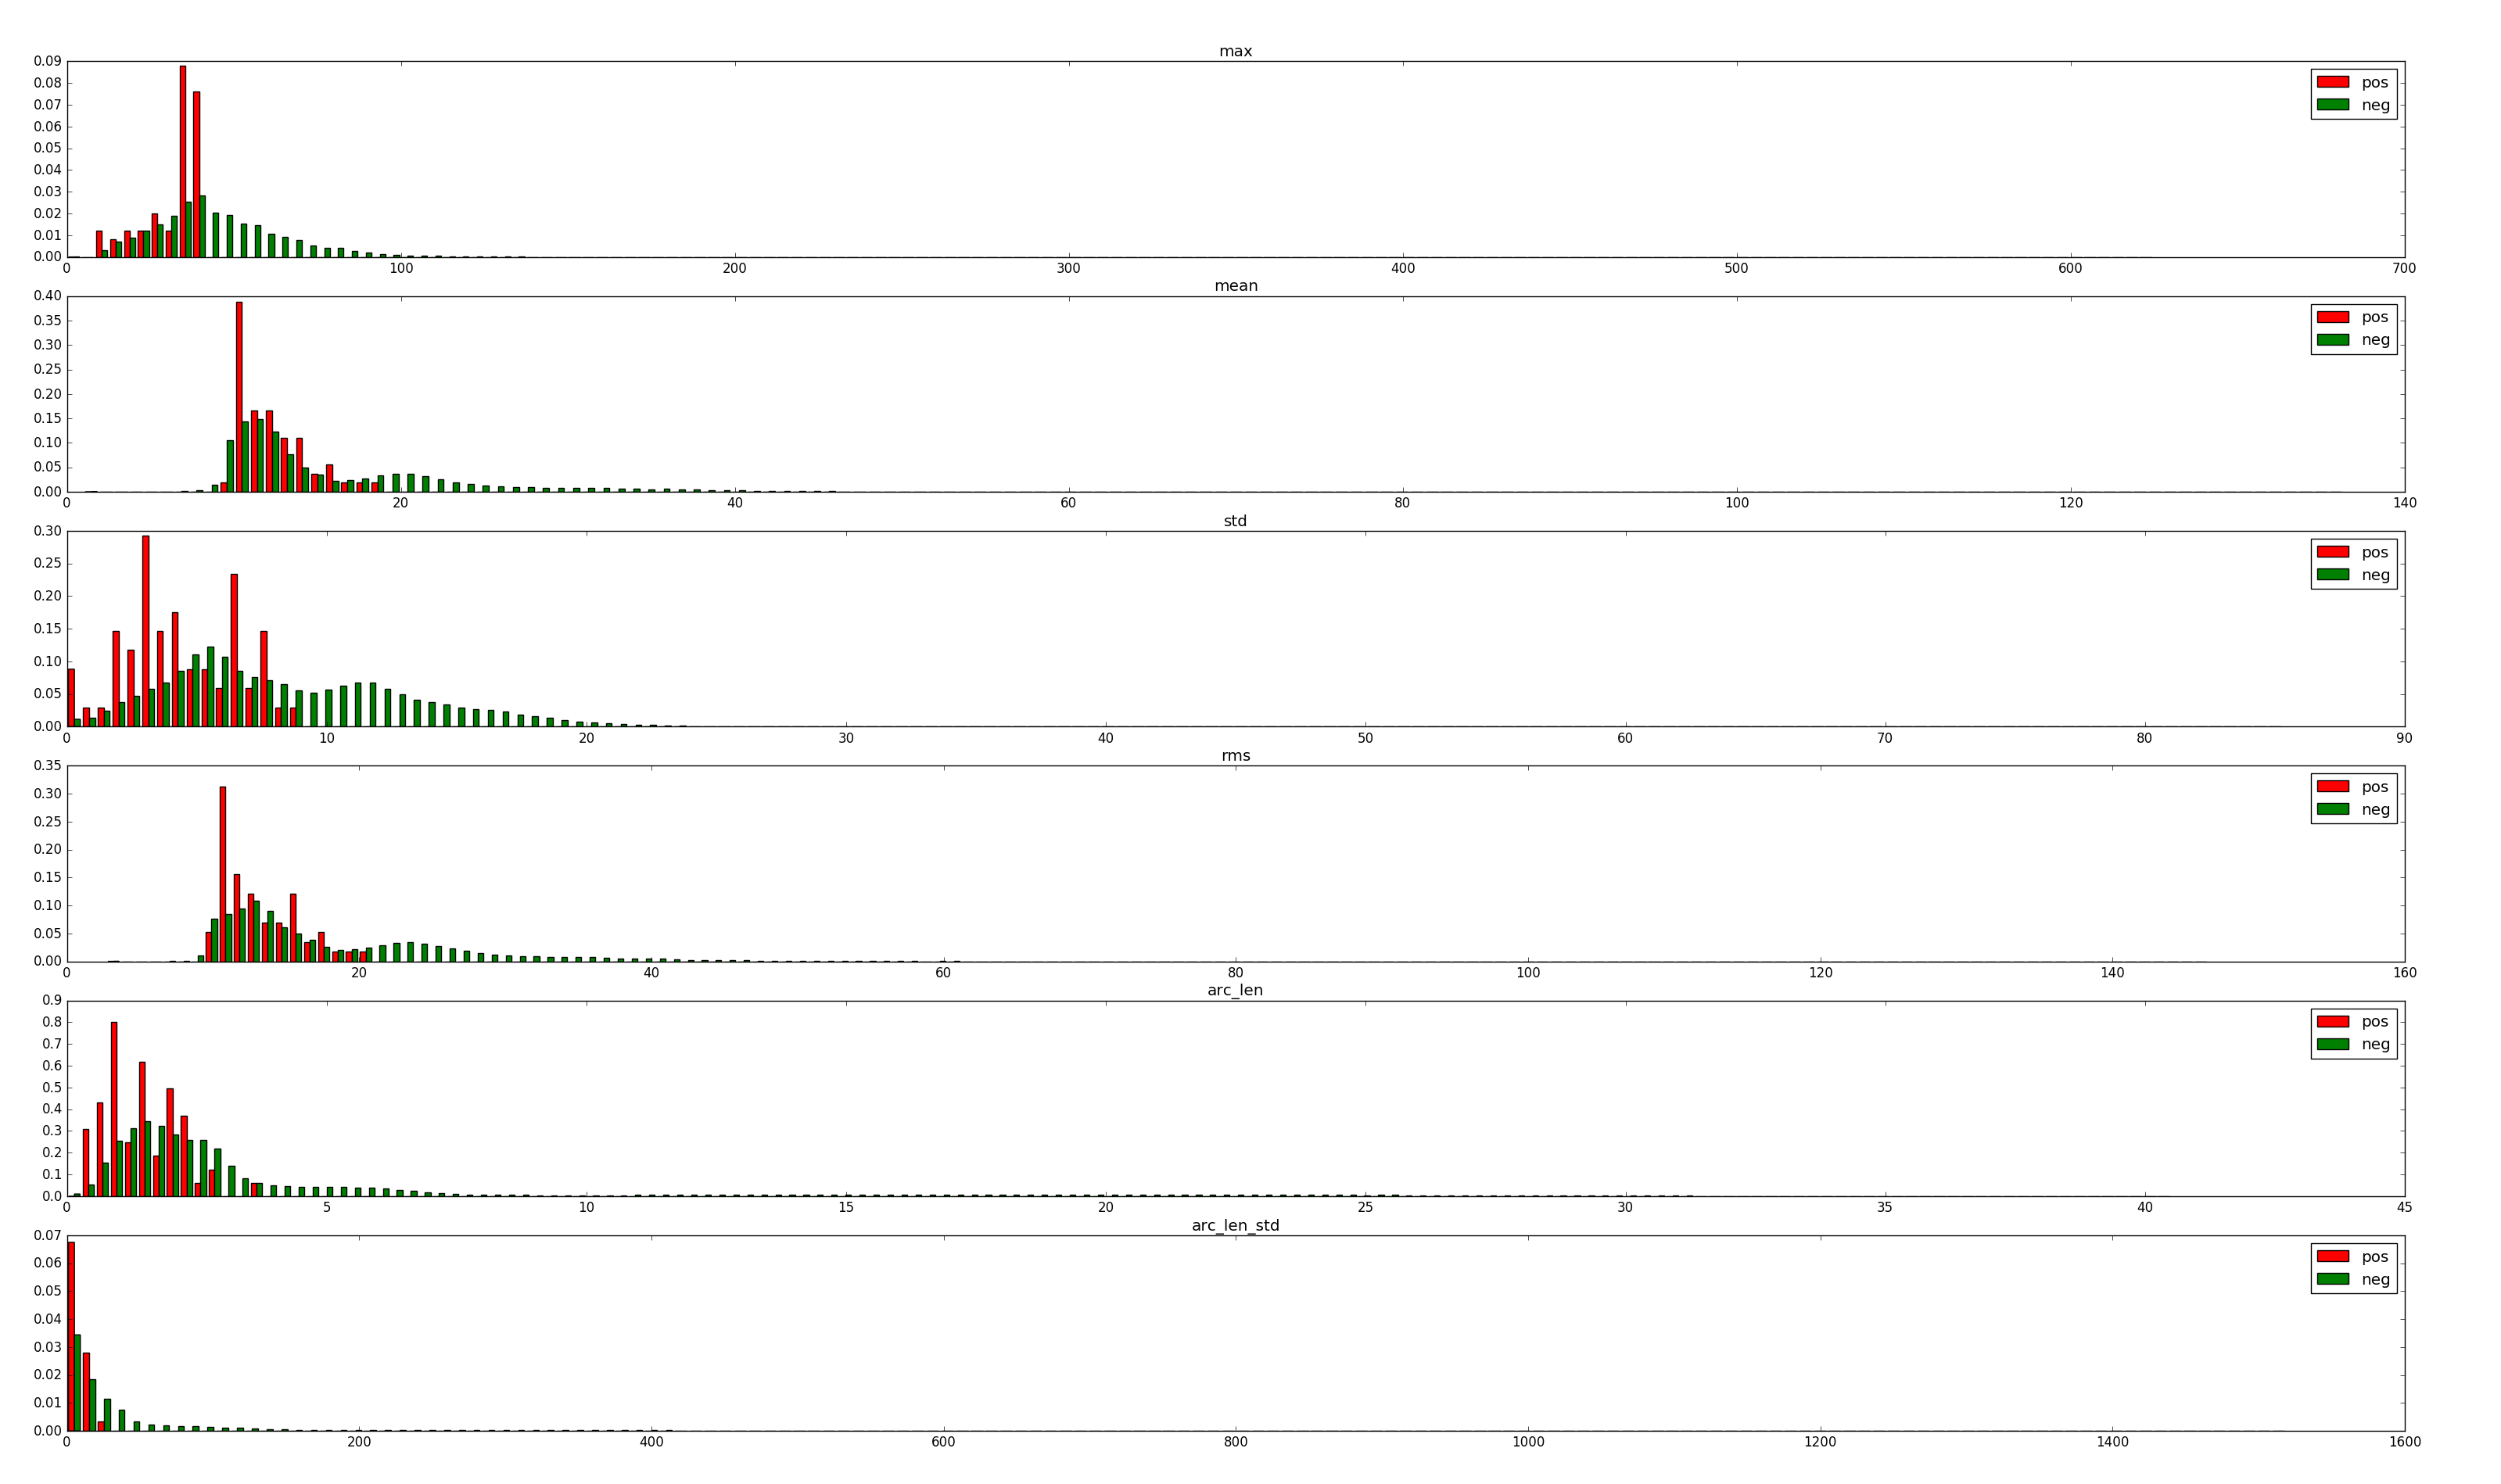
\includegraphics[width=\textwidth]{hist_features_before_win_size_1_2.png}
% \end{minipage}
% \end{center}
% \caption{Histogram for each of the 6 features for the 1-second window before the~$40 m/s^2$ spike.  The features are listed in the order presented in Section~\ref{s:features}, e.g., the top histogram is for the maximum.  Red bars indicate thefts, and green bars indicate non-theft windows.}
% \label{fig:beforehist}
% \begin{center}
% \begin{minipage}
% 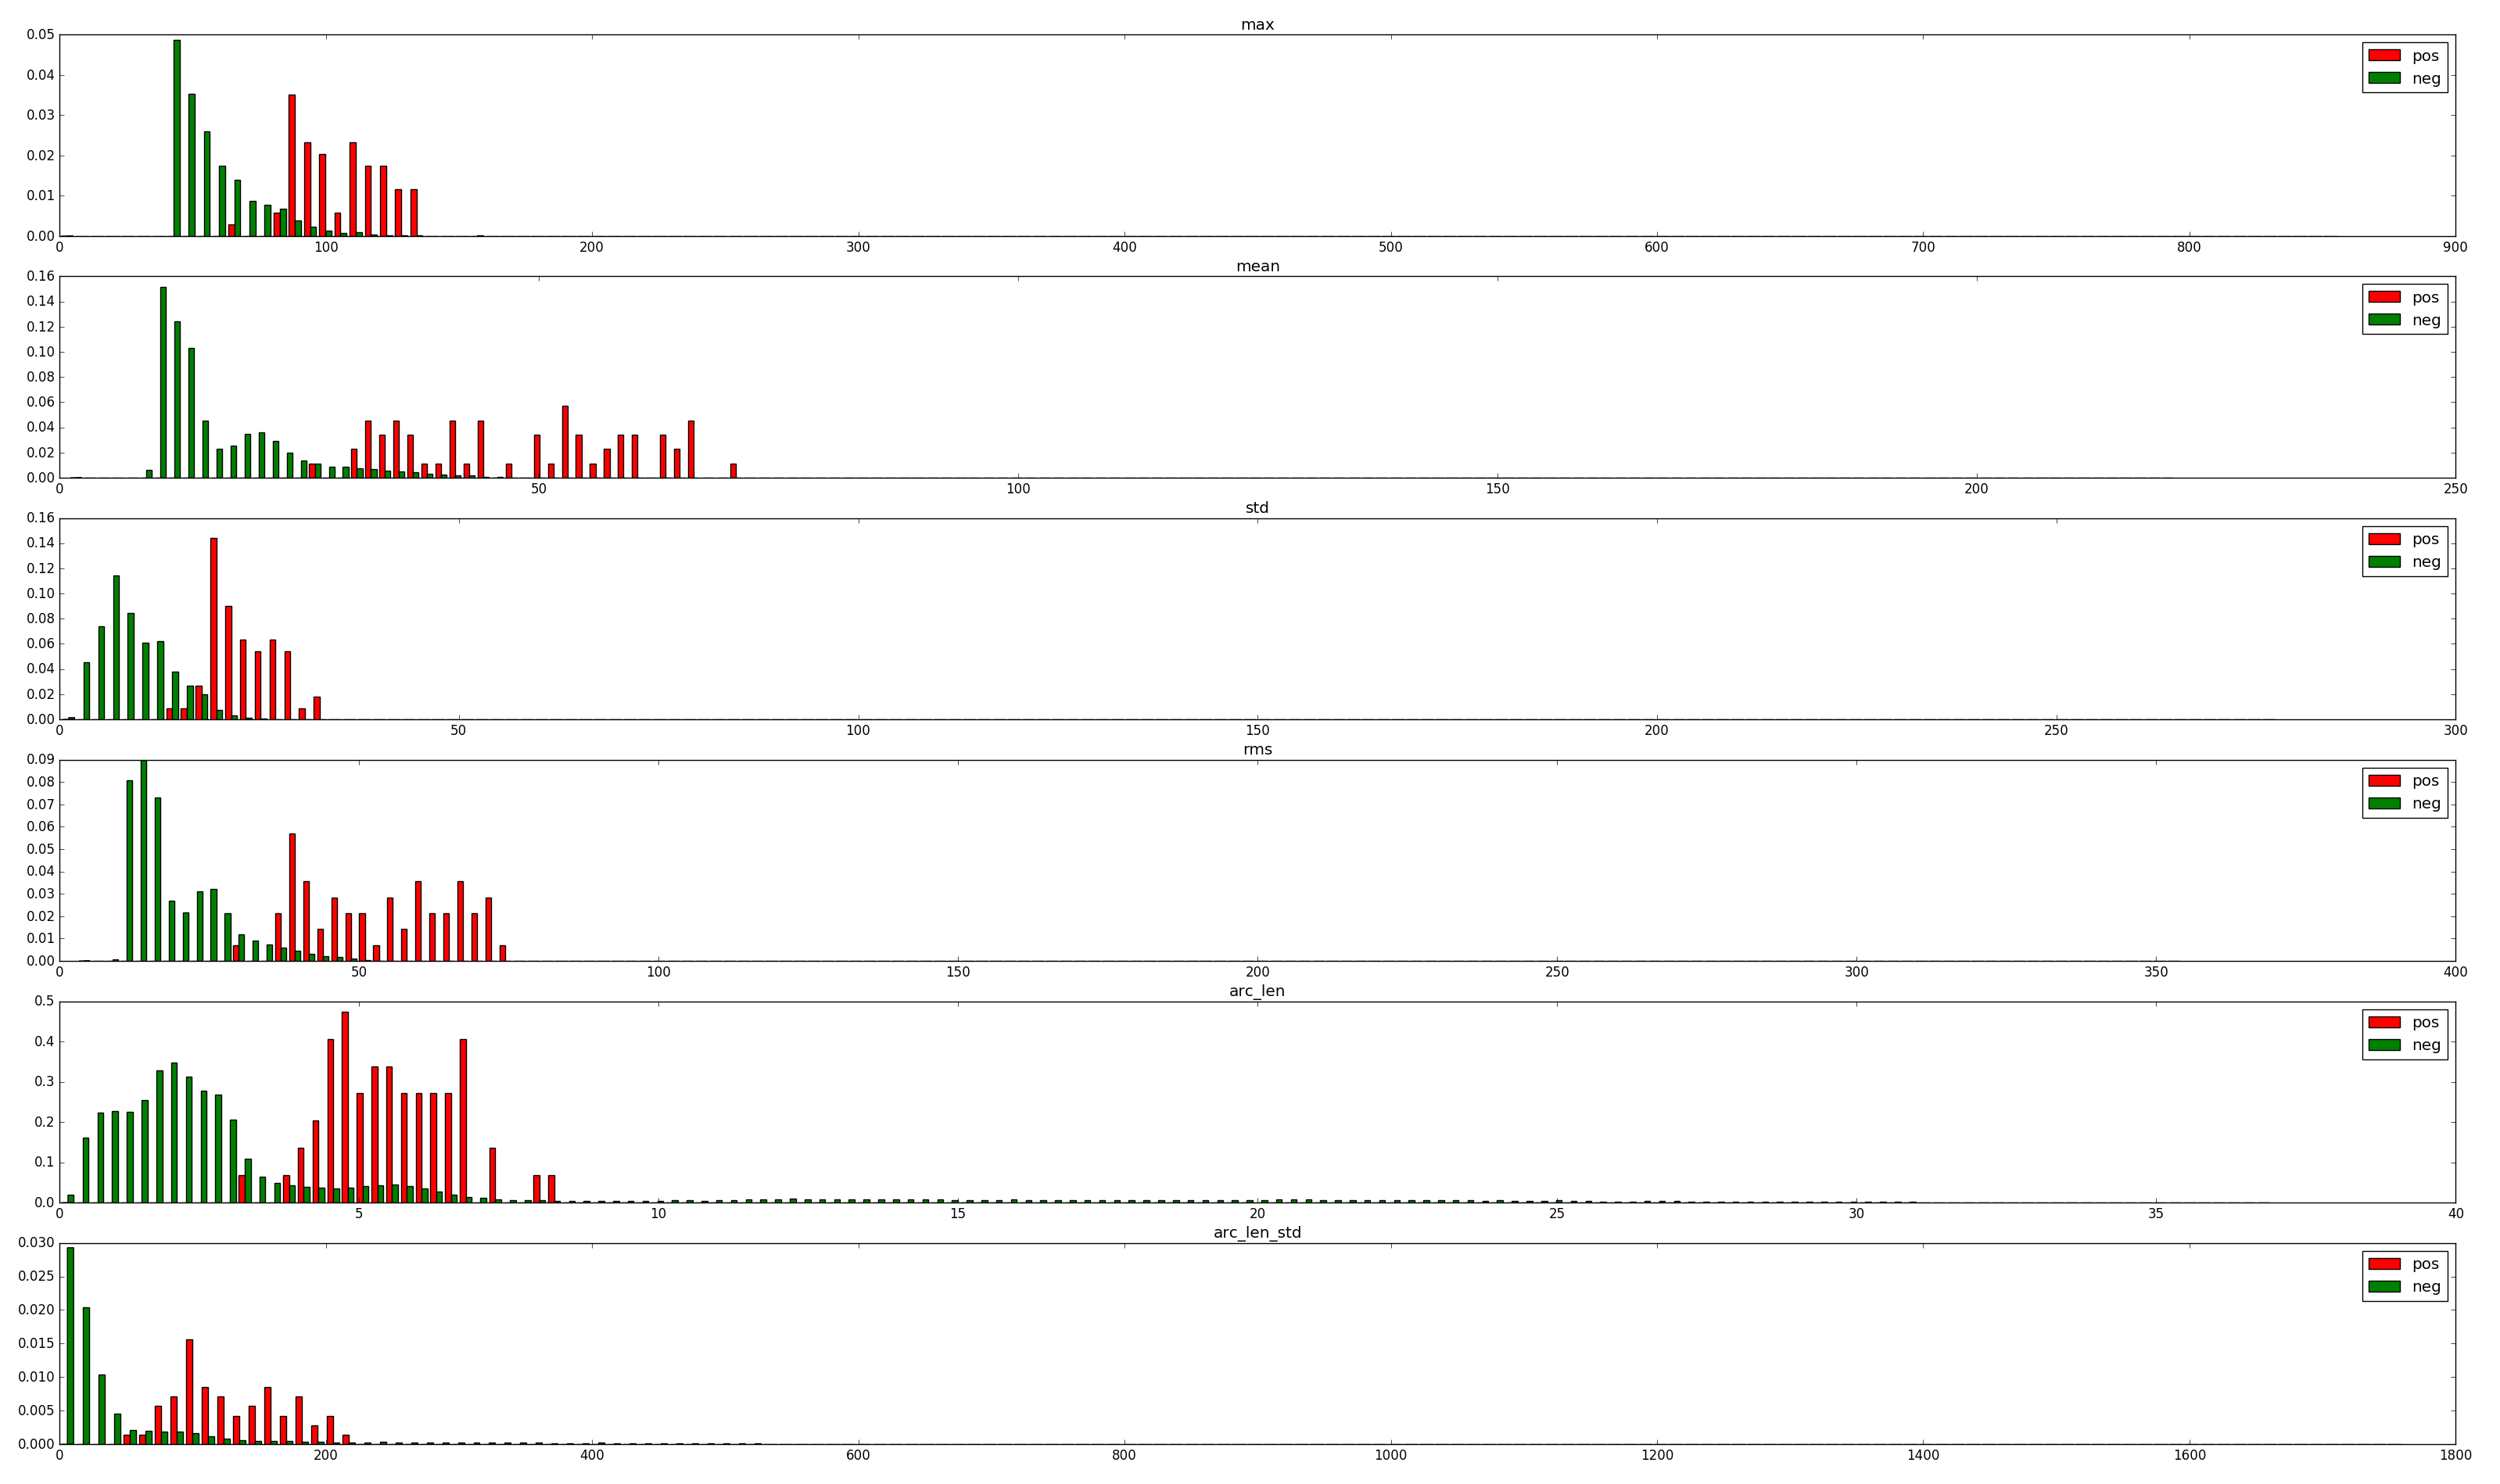
\includegraphics[width=\textwidth]{hist_features_after_win_size_1_2.png}
% \end{minipage}
% \end{center}
% \caption{Histogram of feature values in the 2-second window after the~$40 m/s^2$ spike.}
% \label{fig:afterhist}

% \end{figure*}


\begin{figure*}[t]
\centering
\begin{minipage}[t]{\columnwidth}
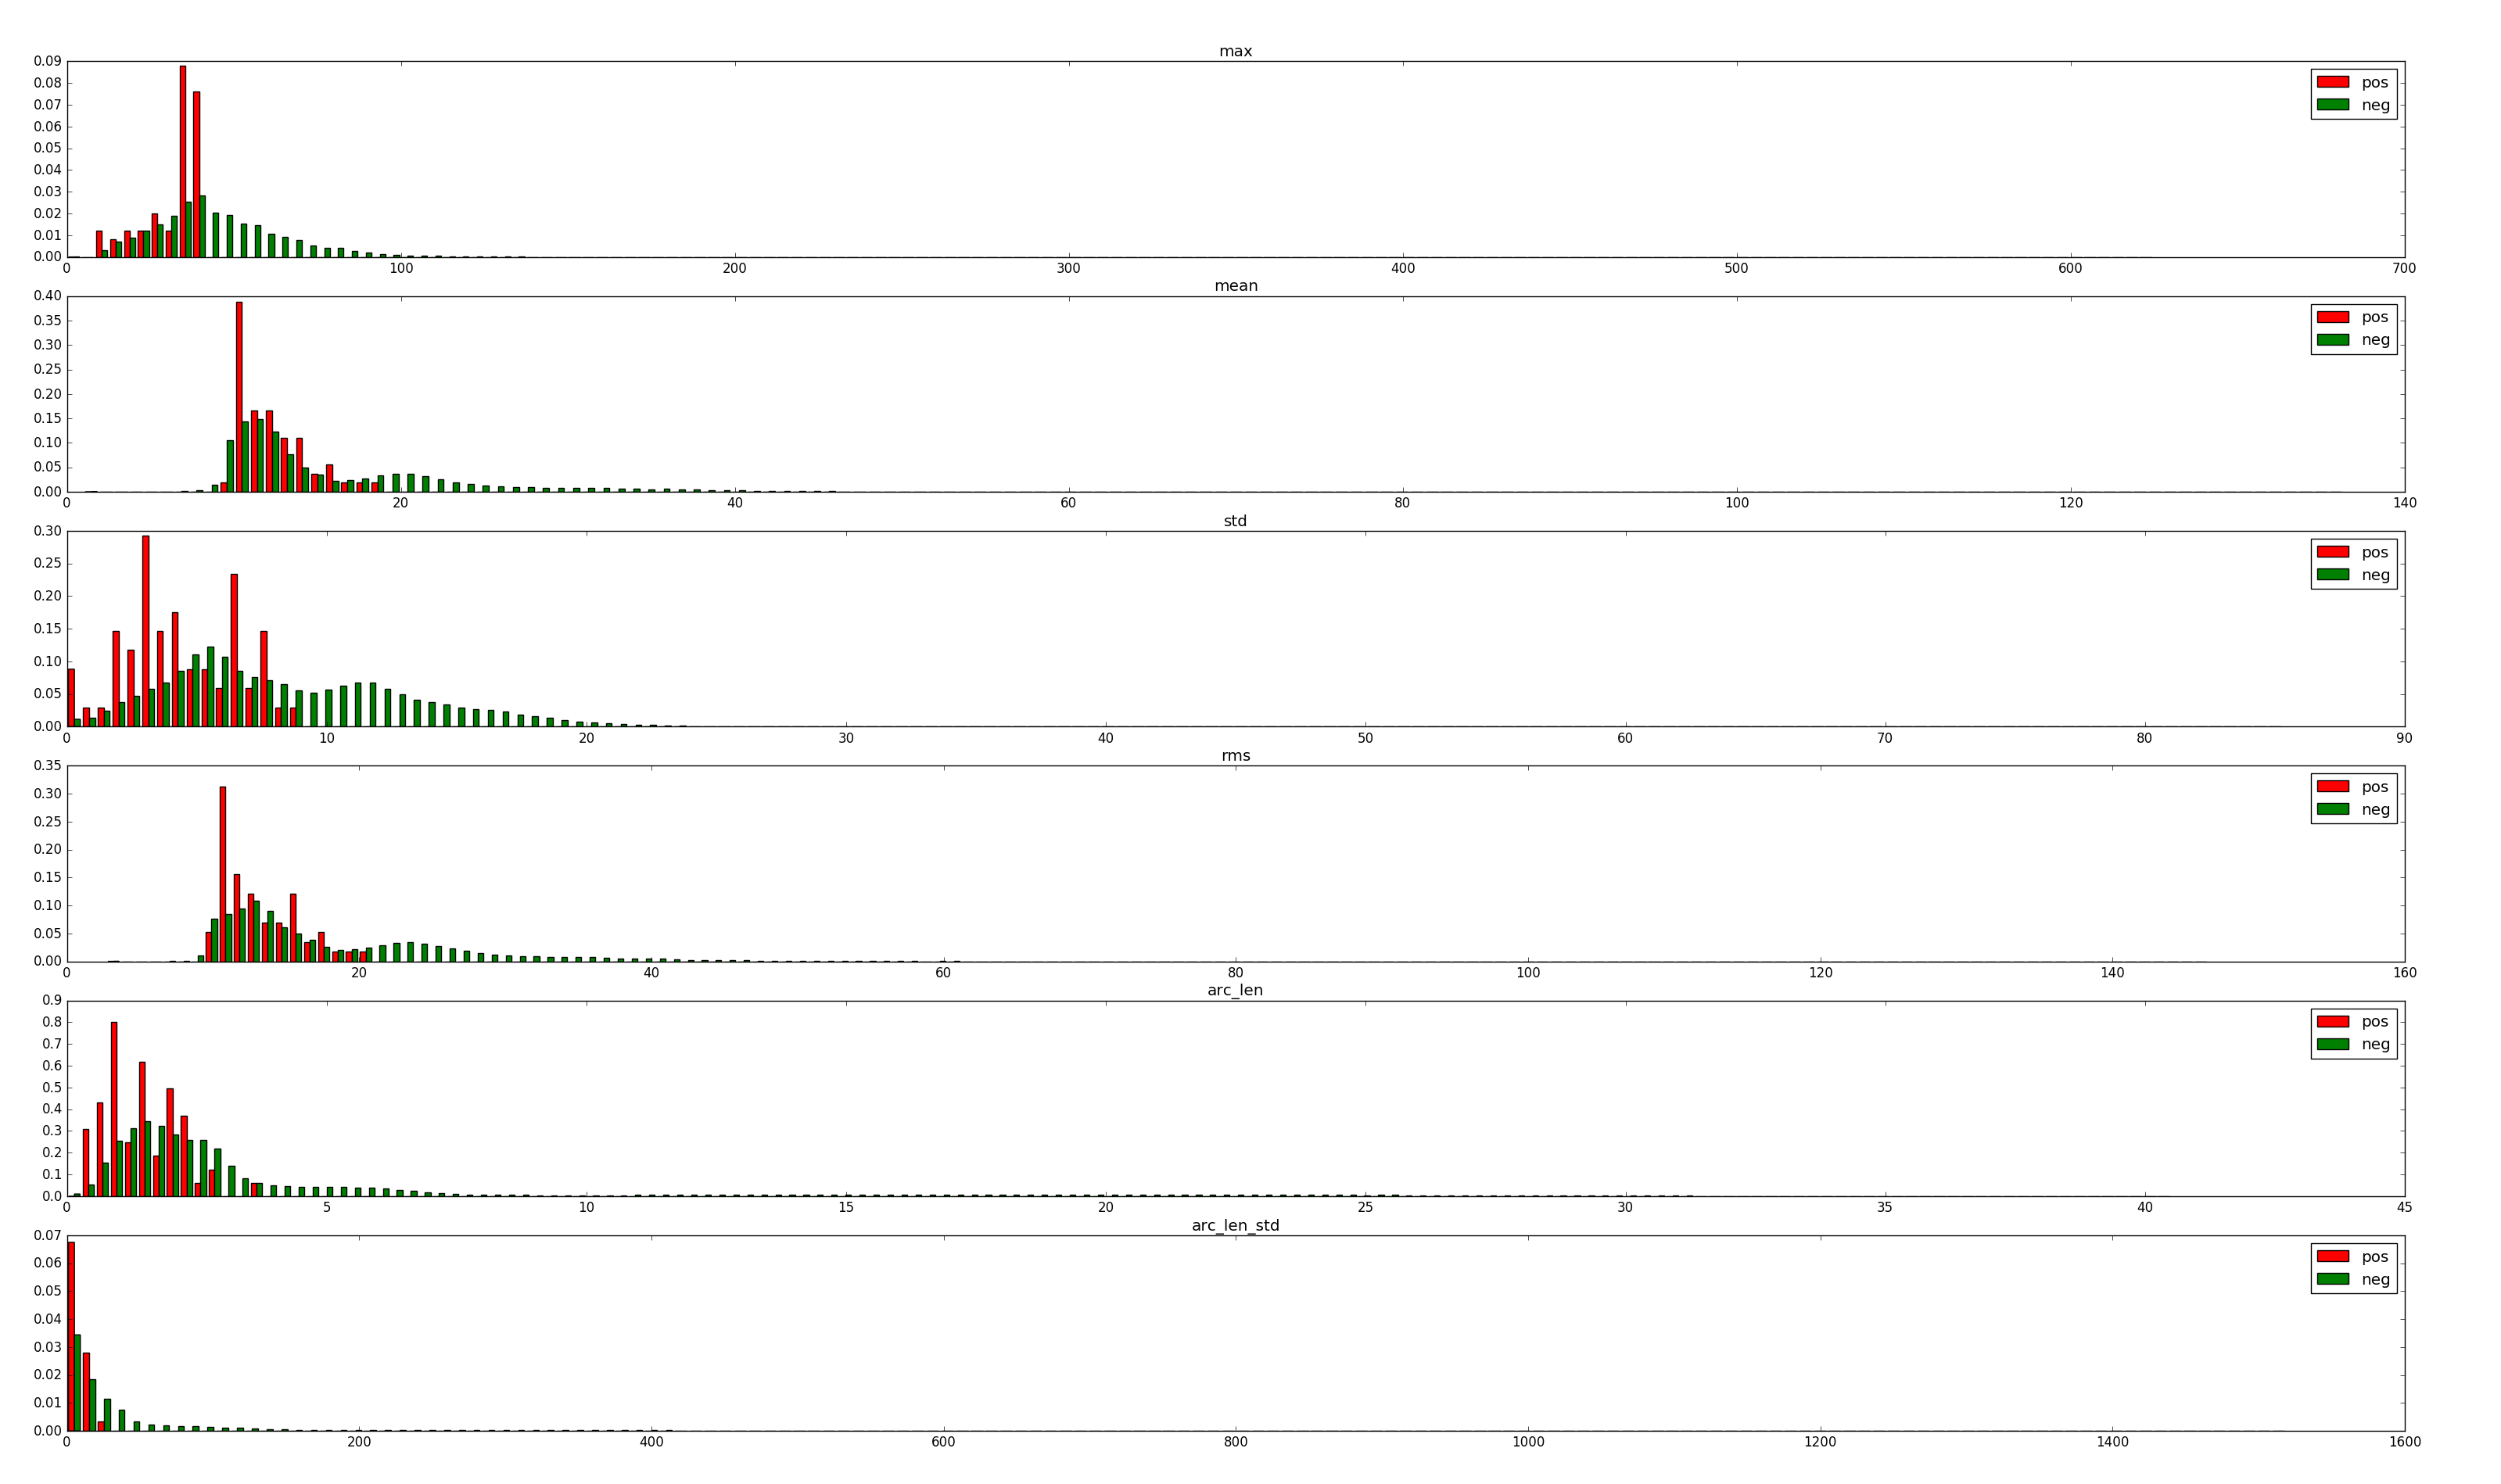
\includegraphics[width=\columnwidth]{hist_features_before_win_size_1_2.png}
\caption{Histogram for each of the 6 features for the 1-second window before the~$40 m/s^2$ spike.  The features are listed in the order presented in Section~\ref{s:features}, e.g., the top histogram is for the maximum.  Red bars indicate thefts, and green bars indicate non-theft windows.}
\label{fig:beforehist}
\end{minipage}
\hfill
\begin{minipage}[t]{\columnwidth}
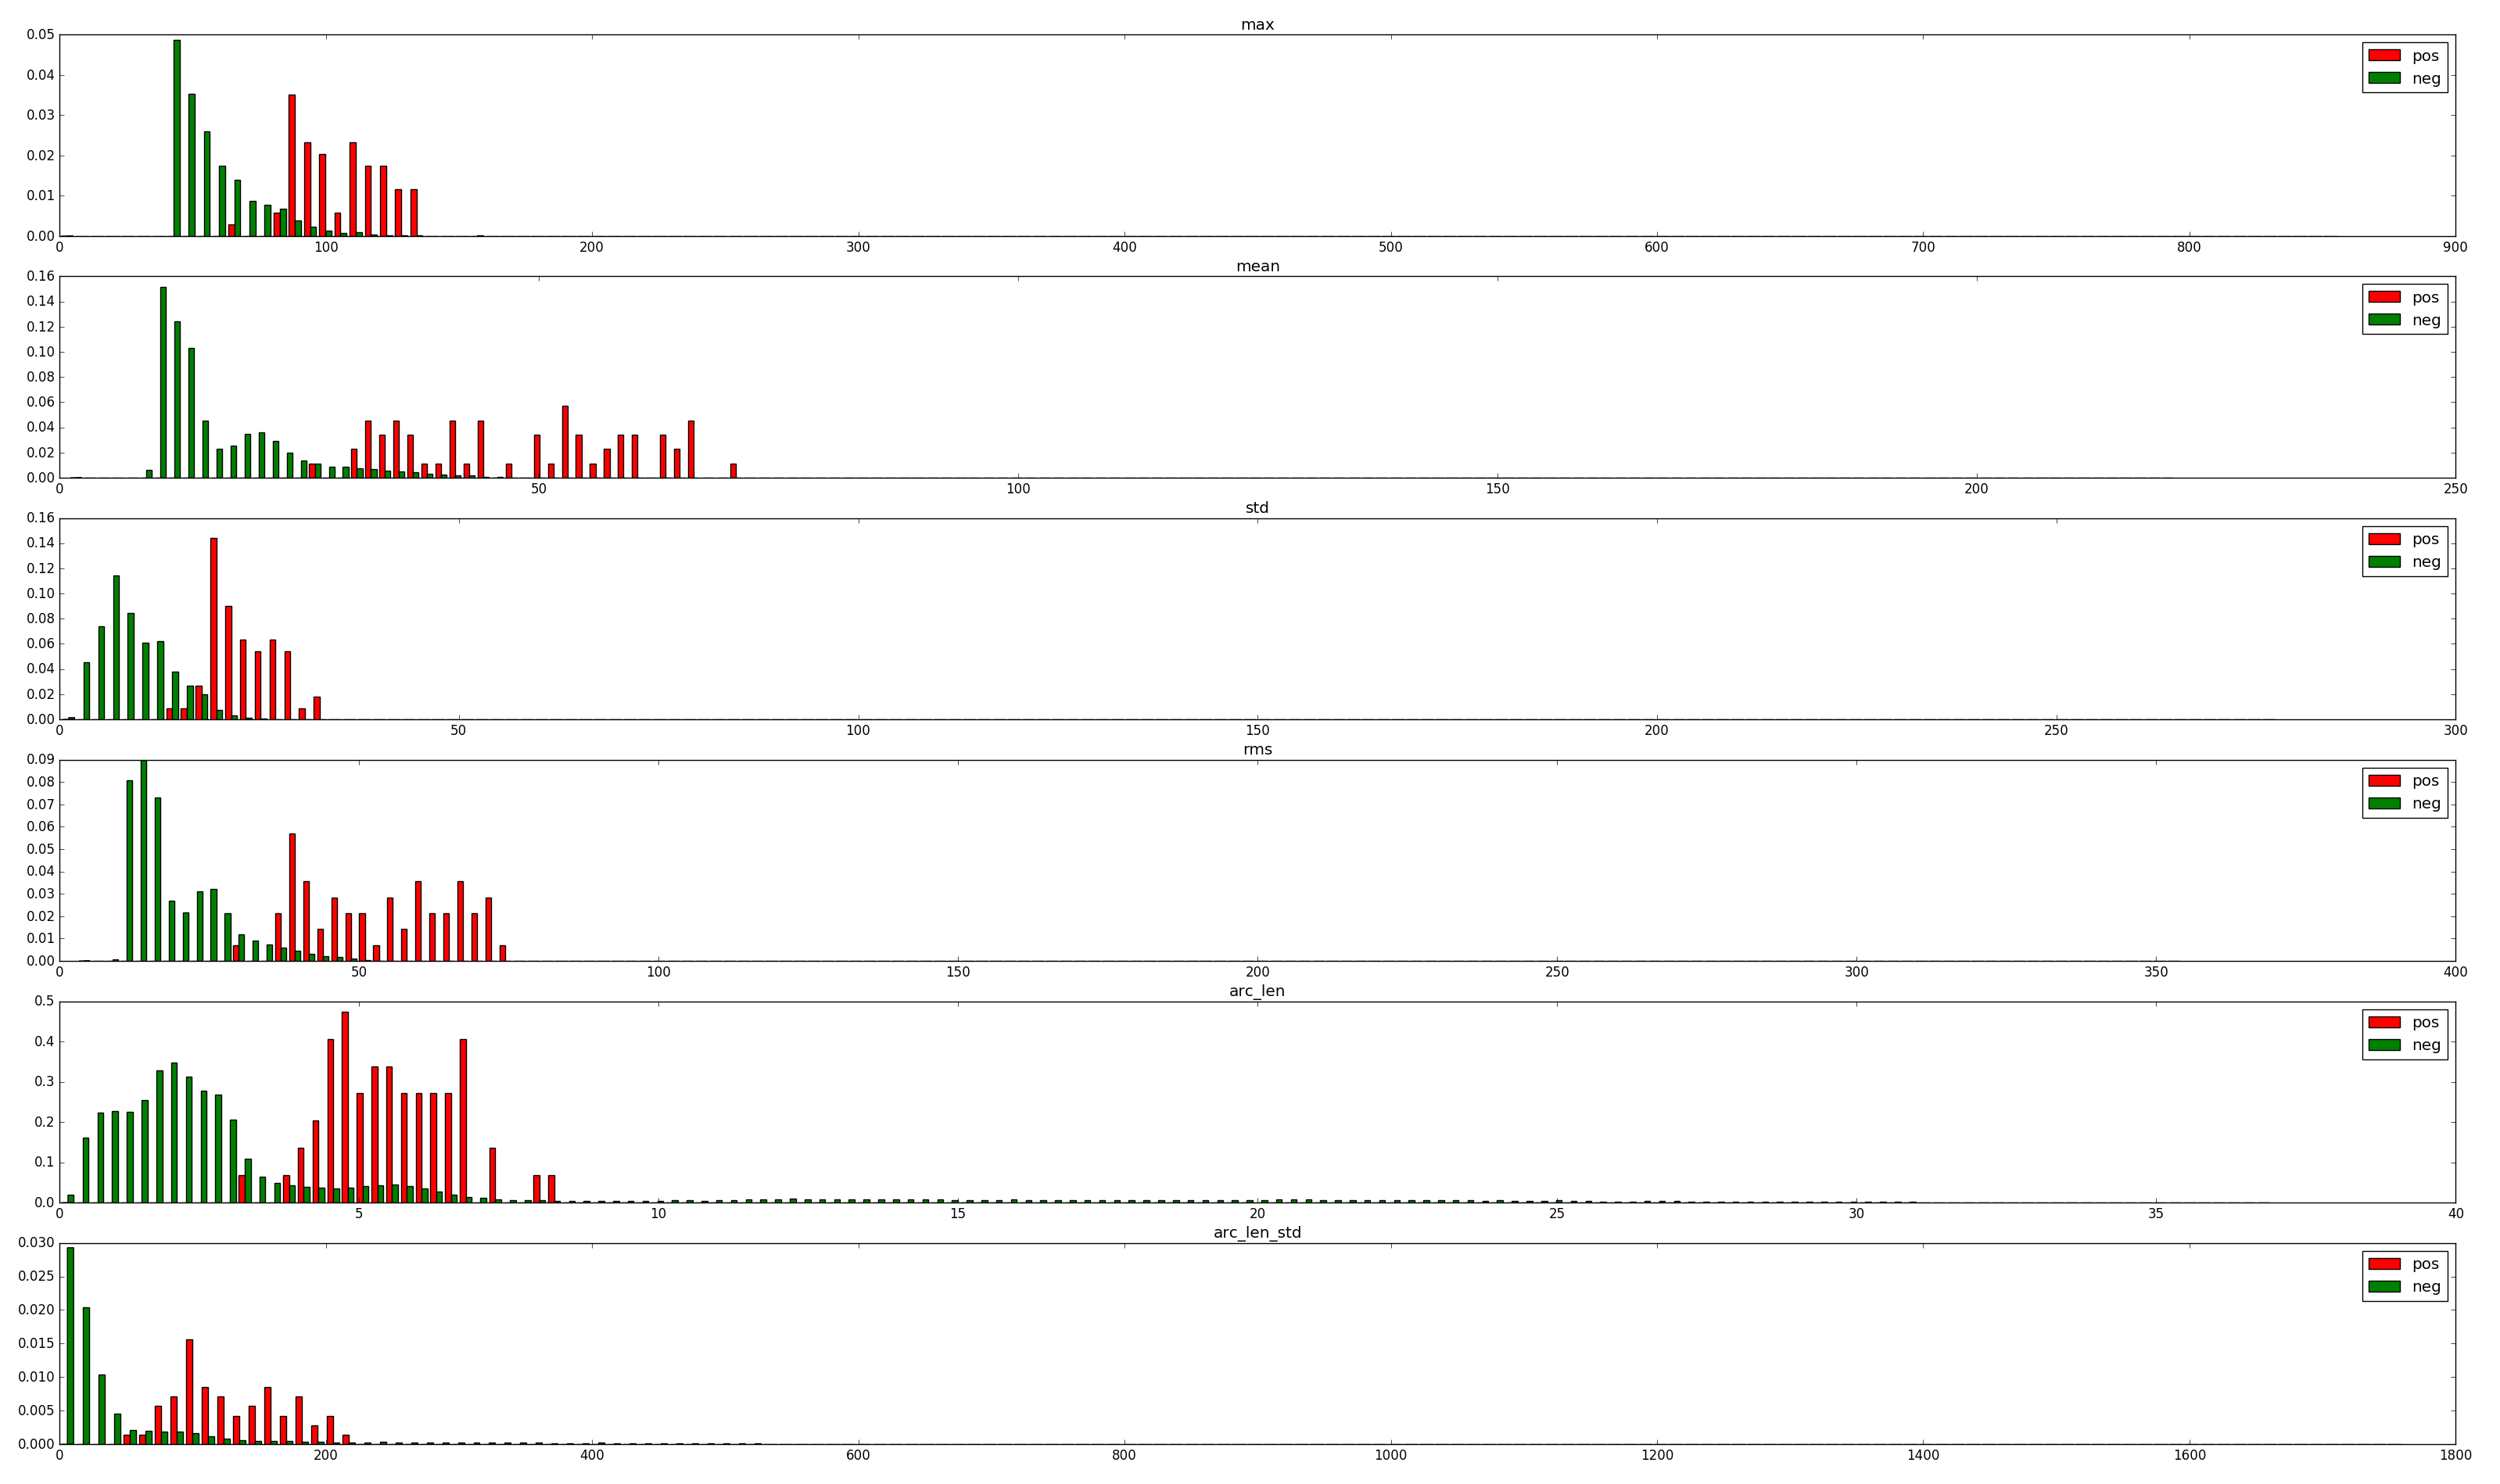
\includegraphics[width=\columnwidth]{hist_features_after_win_size_1_2.png}
\caption{Histogram of feature values in the 2-second window after the~$40 m/s^2$ spike.}
\label{fig:afterhist}
\end{minipage}
\end{figure*}

% \begin{figure*}[t]
% \begin{center}
% 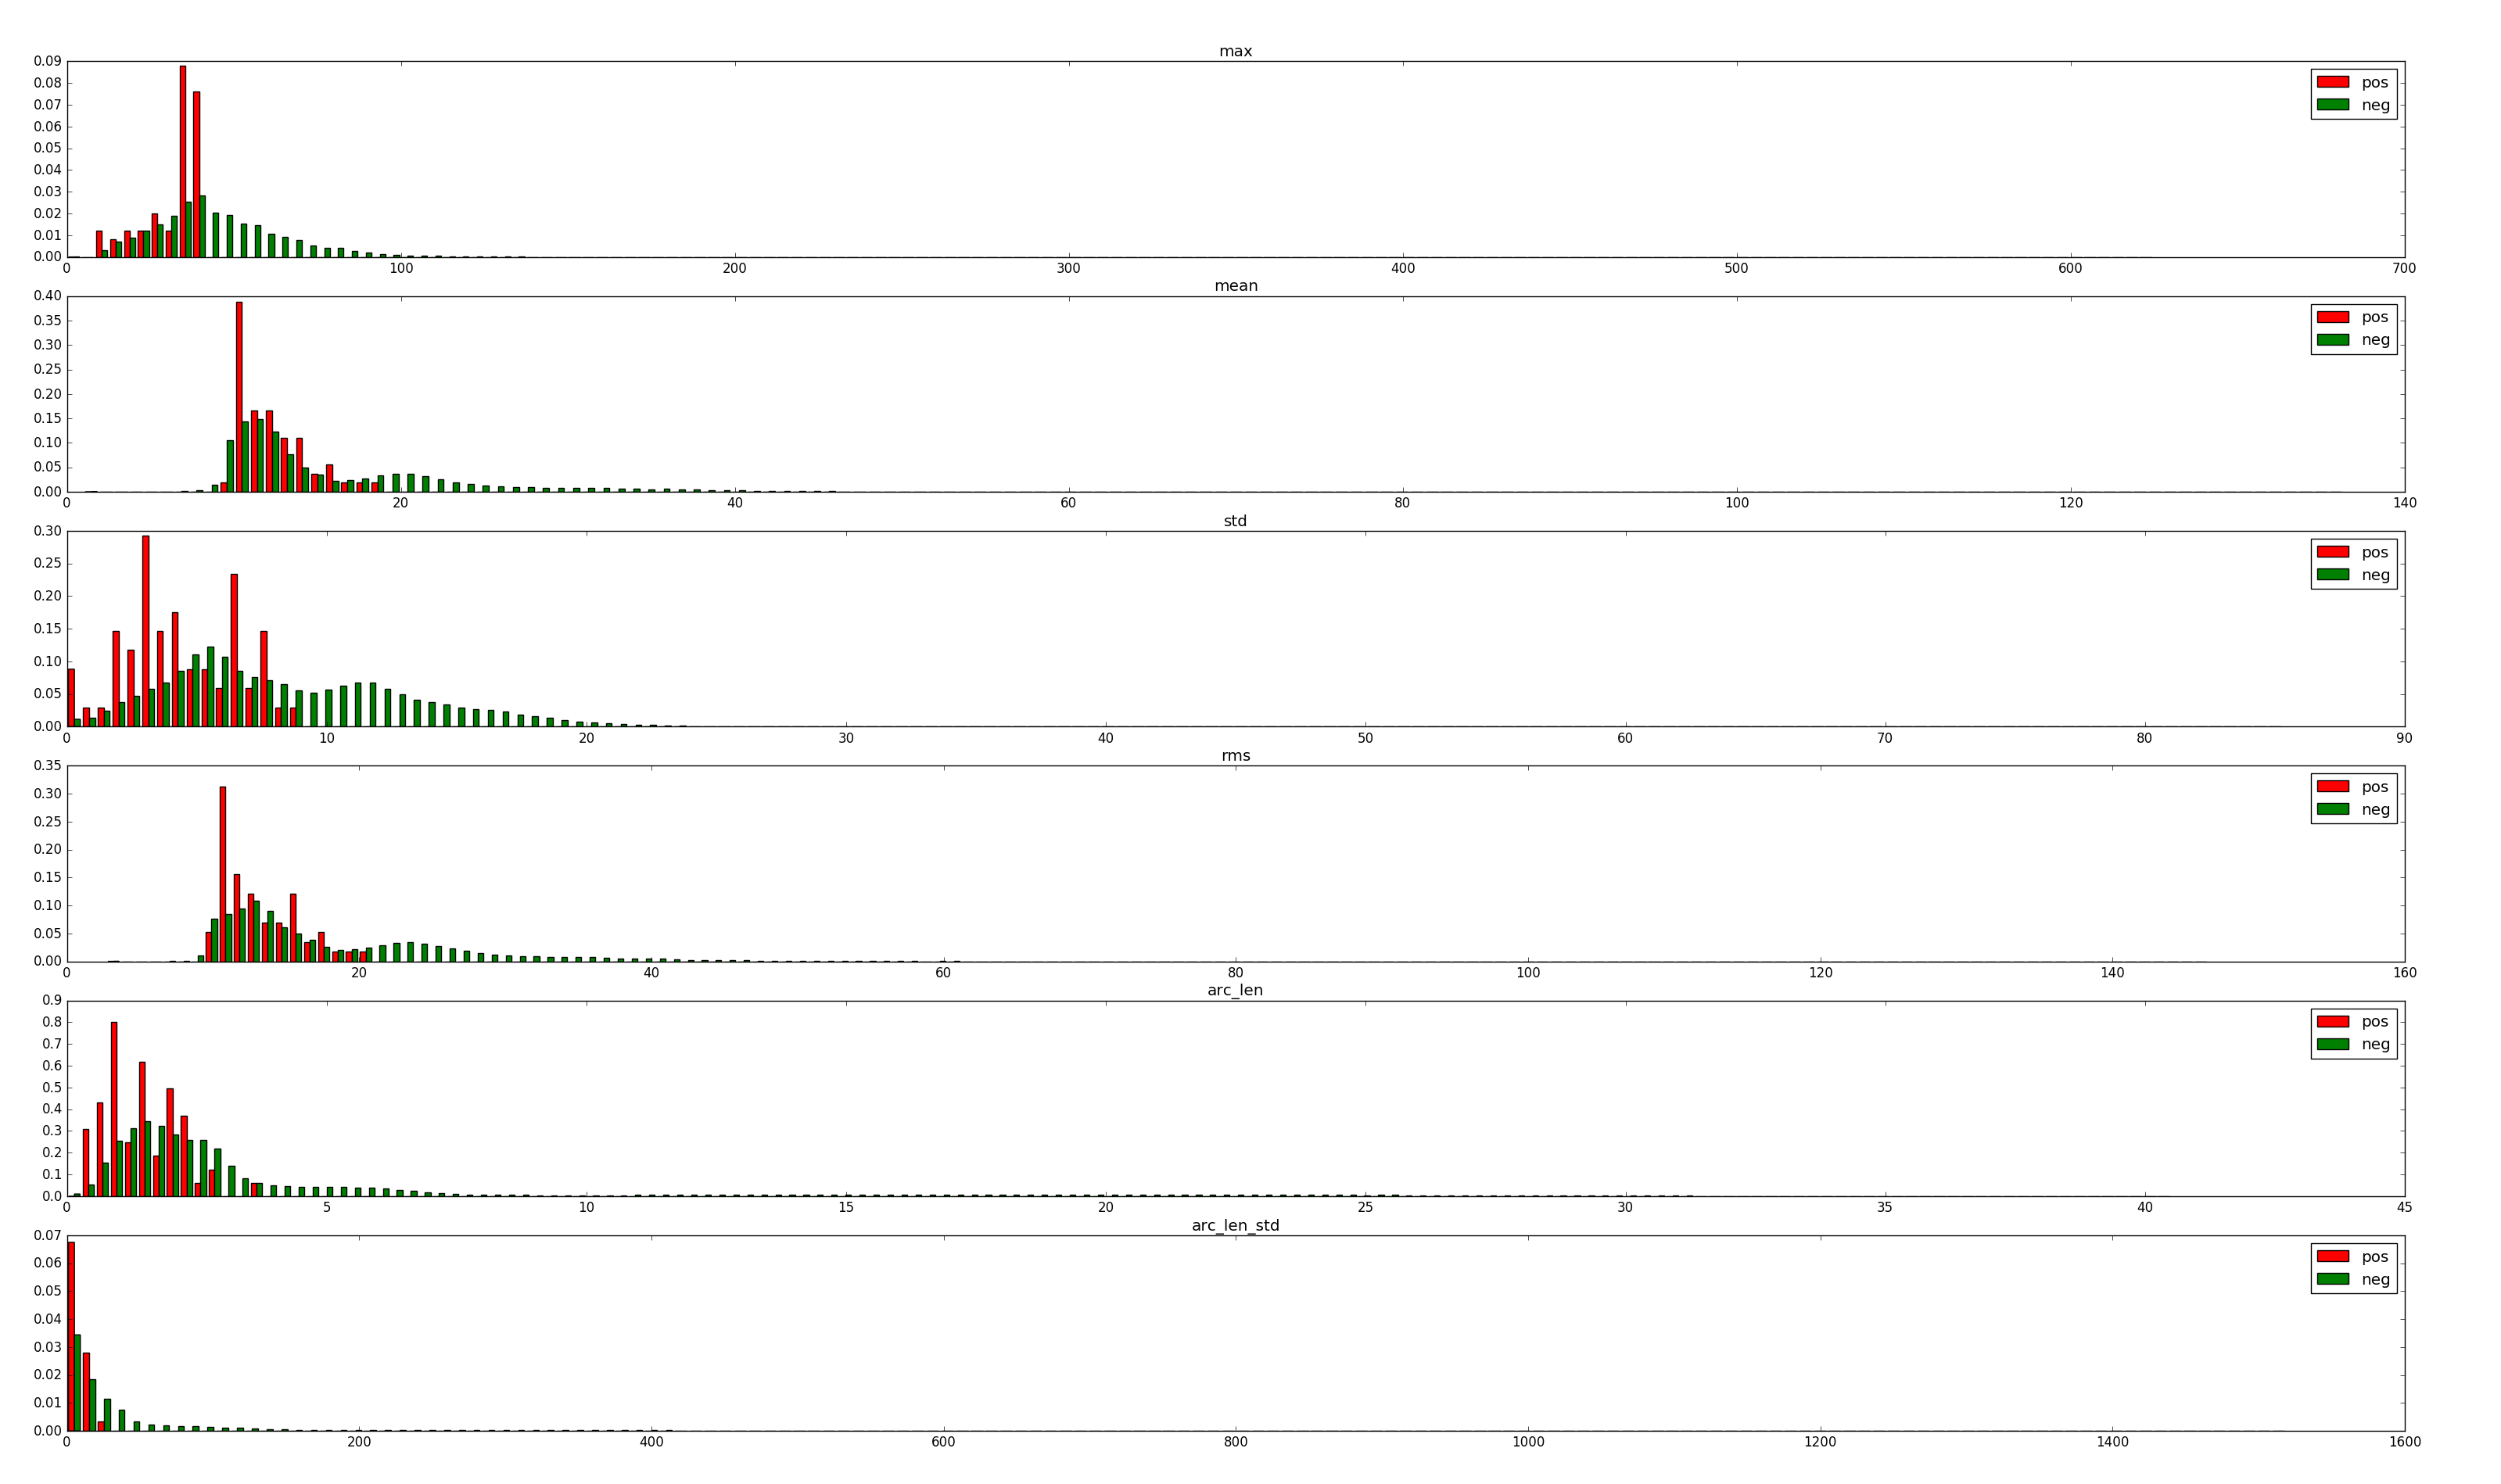
\includegraphics[width=\textwidth]{hist_features_before_win_size_1_2.png}
% \end{center}
% \caption{Histogram for each of the 6 features for the 1-second window before the~$40 m/s^2$ spike.  The features are listed in the order presented in Section~\ref{s:features}, e.g., the top histogram is for the maximum.  Red bars indicate thefts, and green bars indicate non-theft windows.}
% \label{fig:beforehist}
% \end{figure*}

% \begin{figure*}[t]
% \begin{center}
% 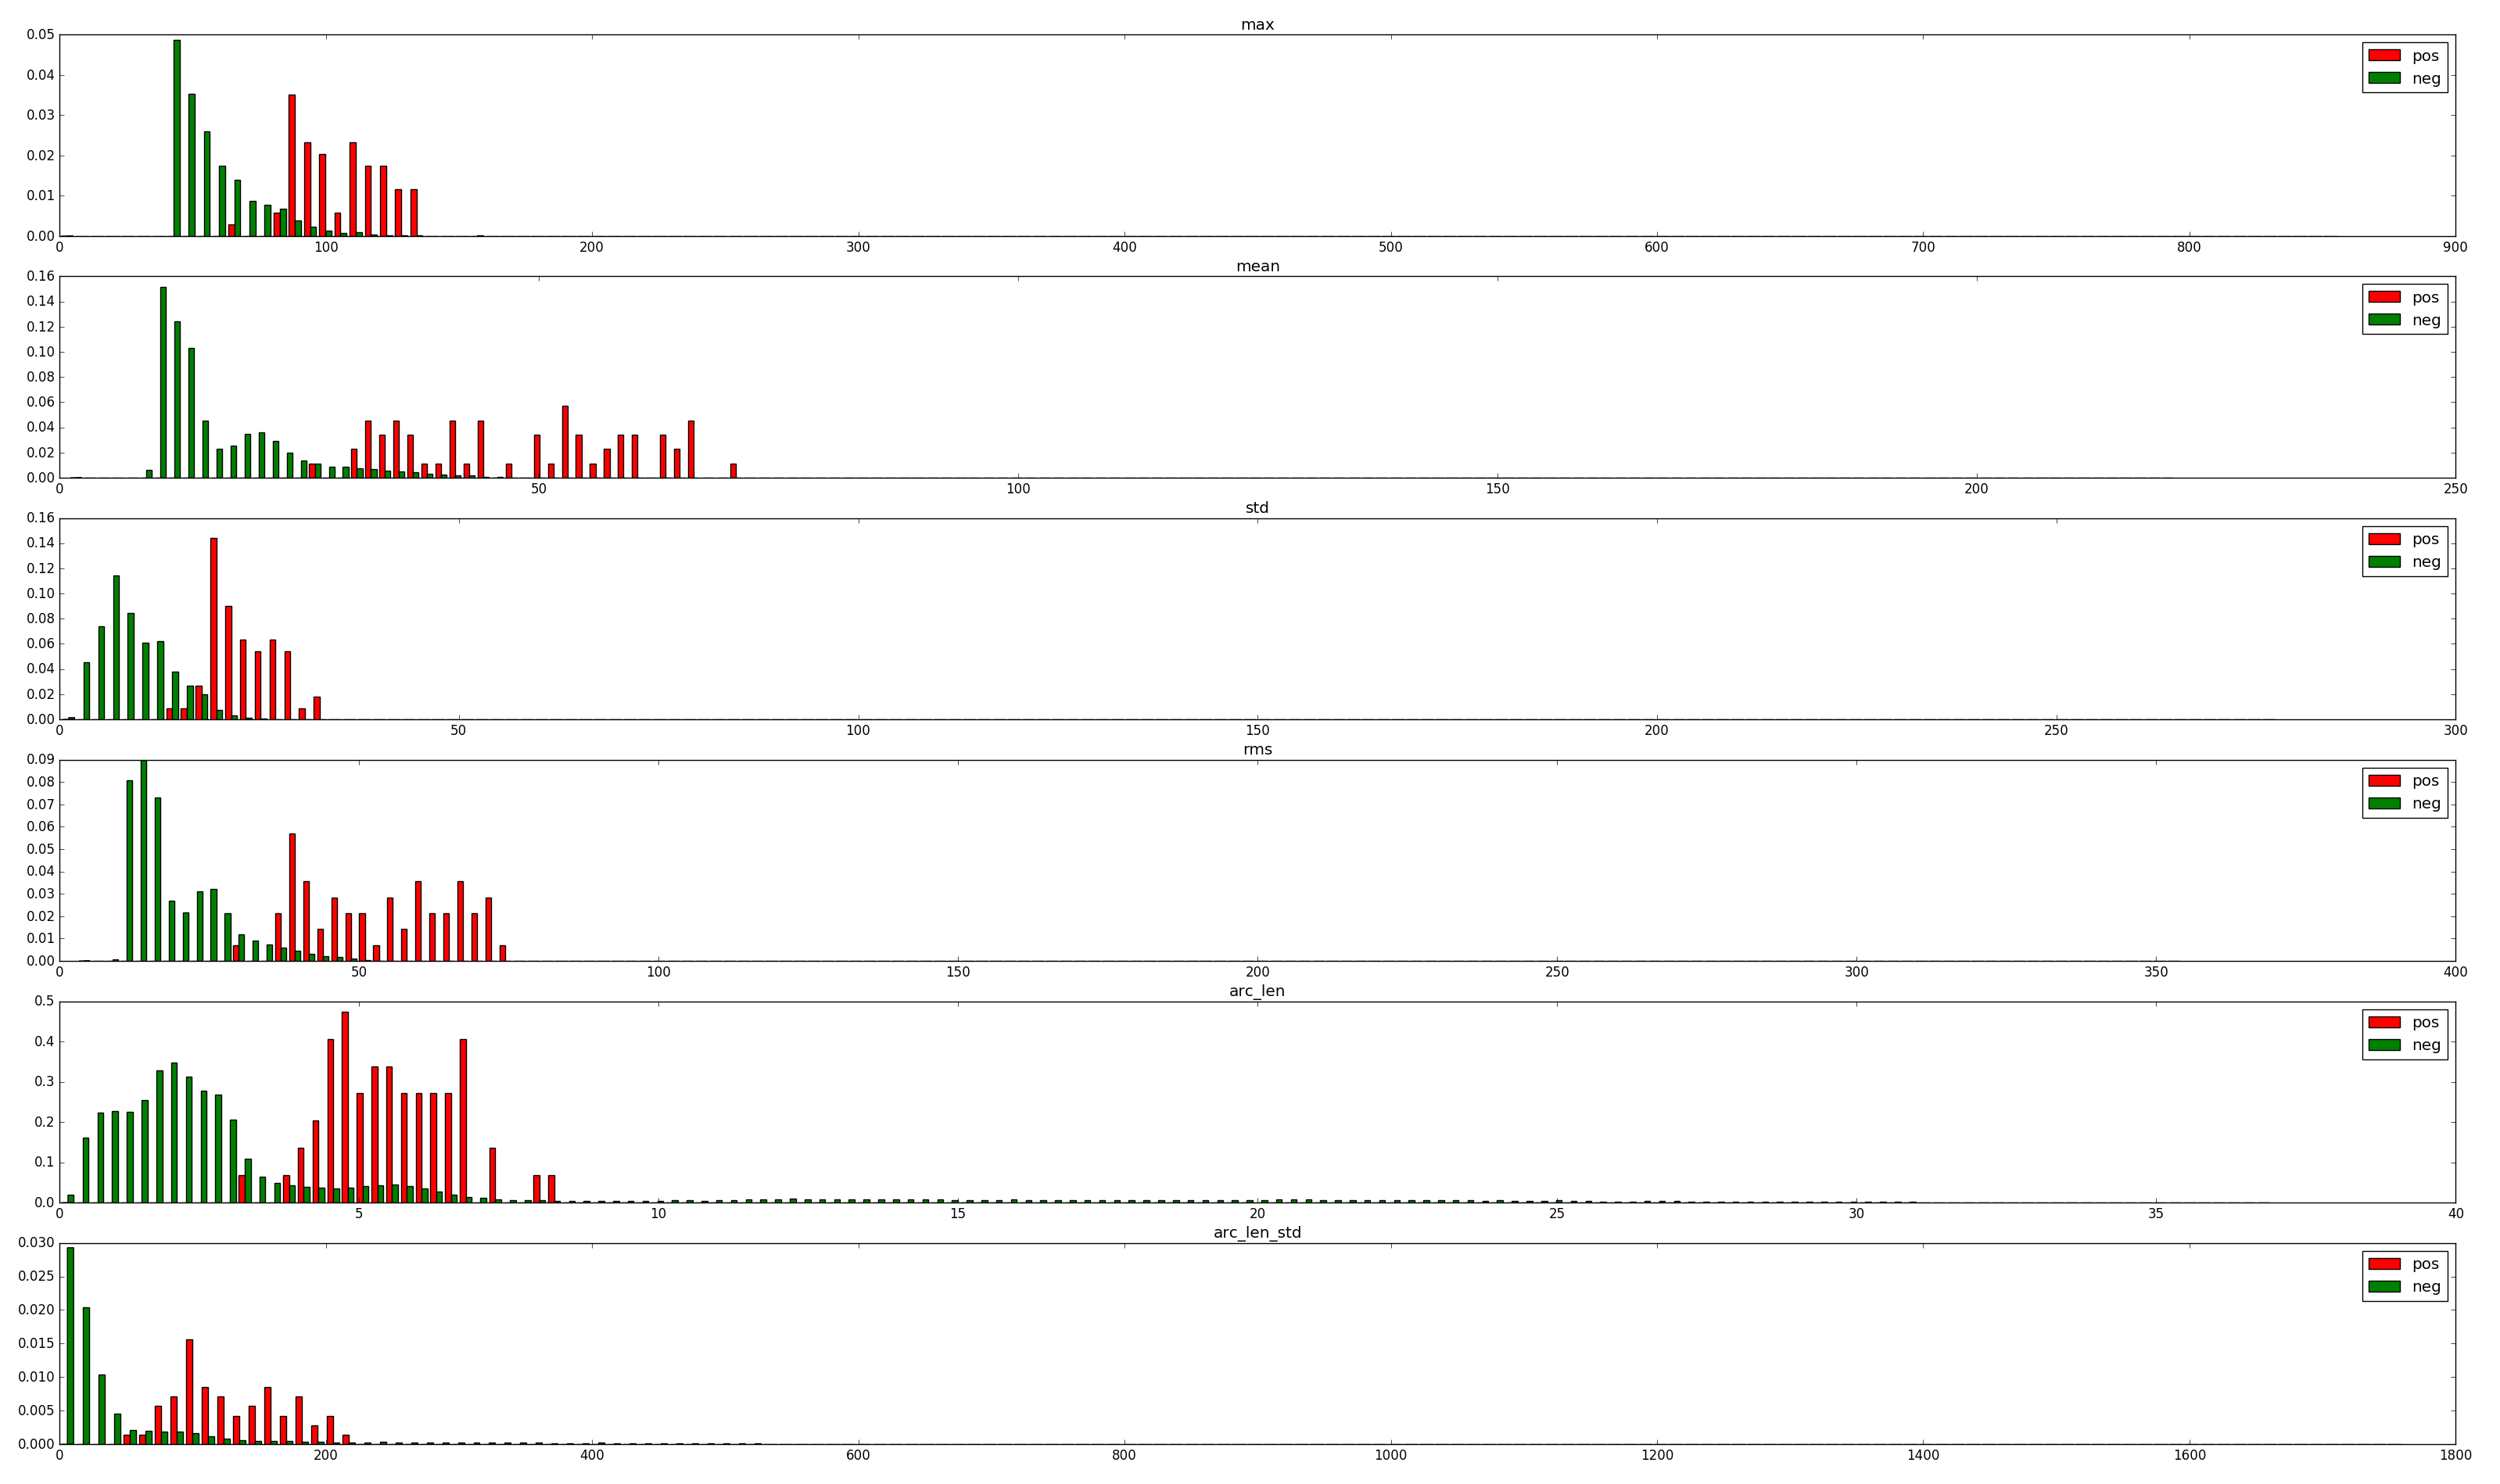
\includegraphics[width=\textwidth]{hist_features_after_win_size_1_2.png}
% \end{center}
% \caption{Histogram of feature values in the 2-second window after the~$40 m/s^2$ spike.}
% \label{fig:afterhist}
% \end{figure*}

To compare the performance of random forests and logistic regression, we fine tuned the class weights for the logistic regression classifier to lower its true positive rate until it is approximately the same as the random forests classifier, then we compared the number of false positive instances of the two classifiers.
We find that logistic regression has 14 false positive instances at a 67\% true positive rate (25 true positive instances),
while random forests has 15 false positive instances at a 62\% true positive rate (23 true positive instances).
Thus the performance of the two classifiers seems comparable in this regime.
The advantage of logistic regression is that we found adjusting class weights was more effective at controlling the false-positive/false-negative tradeoff for the logistic regression classifier.
The Receiver Operating Characteristic (ROC) curves for the logistic regression and random forests classifiers are shown in Figure~\ref{fig:roc}.

\begin{figure}[t]
\begin{center}
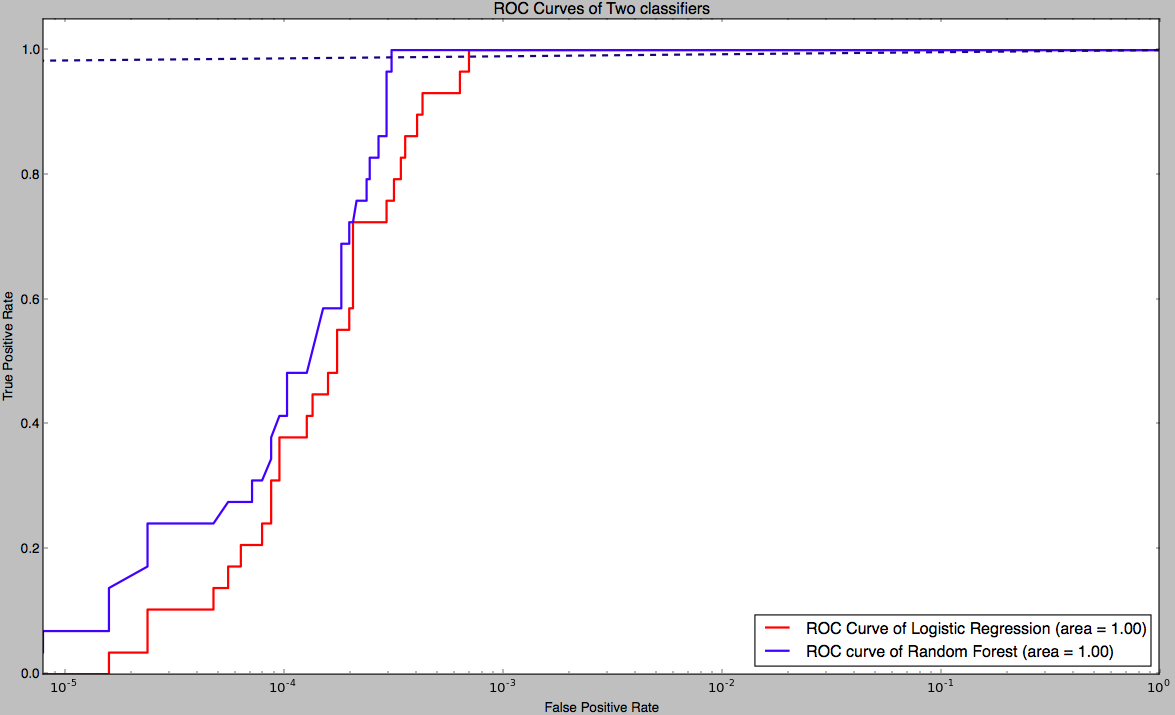
\includegraphics[width=1.0\columnwidth]{roc_curves_log_line.png}
\end{center}
\caption{ROC curves of logistic regression and random forests. The x-axis is in logarithmic scale.}
\label{fig:roc}
\end{figure}




\begin{acks}
% TODO: For the submission, don't include acknowledgments since they would most likely deanonymize you.
\begin{comment}
\textcolor{red}{Comment out for double blind review}. 

The authors would like to thank Prakash P. Bhasker and Micah J. Sheller for proivding with the Android sensor monitoring software, Jennider Chen from the Good Research for her assistance on conducting the user study, and Irwin Reyes, David Fifield \textcolor{red}{Who else gives feedback to draft} for giving feedback to our paper drafts. 
This research was conducted at The Intel Science and Technology Center for Secure Computing (http://scrub.cs.berkeley.edu/) at UC Berkeley. 
The work is supported by \textcolor{red}{What Grants and Funds}. 
\end{comment}
\end{acks}
 % TODO: replace with your brilliant paper!

\bibliographystyle{ACM-Reference-Format}
\bibliography{ccs-sample}

\end{document}
